\documentclass[../Head/report.tex]{subfiles}
\begin{document}
\section{Results}
\label{sec:results}

\subsection{Simulation}

This sections includes simulations of the system in Gazebo for a number of different configurations. This will give an indication of the performance of the implementation which is critical before moving on to implement the solution on the actual drone. 

Section \ref{sec:GPS2Vision_pose_estimation} will investigate the performance of the ArUco pose estimation algorithm based on the GPS2Vision marker on the wall to be compared to the ground truth pose of the drone. This will yield an error which is expected to increase as the drone moves further away from the ArUco board. Thus, the maximum allowed distance away from the board can be estimated to insure a reliable GPS to vision transition. To further analyse the reliability of the ArUco pose estimation based on the GPS2Vision board, the rolling average of a sequence of pose estimates is analyzed for fluctuations in the data in Section \ref{sec:rolling_average_aruco_pose_estimation}. 

Section \ref{sec:hold_pose_using_aruco_pose_estimation} will deal with performance evaluation of the control algorithms for pose control by having the drone to hold its current pose in front of the GPS2Vision and landing boards. This will give an indication if further optimizations of the pose have to be performed. Moreover, the ArUco pose estimations will be compared to that of the ground truth to see if the error in the pose estimation is reduced when the number of visible ArUco markers are increased by using different setups of ArUco boards. 

In Section \ref{sec:gps2vision_transition}, the actual GPS2Vision implementation will be analyzed to see how the drone performs in locating the ArUco board, navigate to the board and make the GPS to vision transition in windy conditions for stress analysis. 

Vision based navigation will be analyzed in Section \ref{sec:vision_based_navigation} using a number of different ArUco marker boards located on the ground for pose estimation. To stress test the system, boards with missing markers will be used, which means that the drone has to rely on sensor fusion from IMU and barometer data when no ArUco markers are visible in the image. Further performance evaluations will be based on increased horizontal speed of the drone. 

Finally, the vision based landings will be analyzed in Section \ref{sec:vision_based_landing}. Here all landing stations will be used to compare the precision and accuracy of the landings to evaluate if the number of ArUco markers in the image has an impact on precision and accuracy for both the landing procedure and the actual pose estimation.

\subsubsection{GPS to vision ArUco pose estimation}
\label{sec:GPS2Vision_pose_estimation}

The GPS2Vision pose estimation test is based on a predefined number of waypoints which the drone has to visit while keeping its orientation towards the GPS2Vision marker. The altitude will be 2.5 meters above the ground which is approximately the same as the origin of the GPS2Vision board. At each waypoint, the drone estimates the pose of the board for five seconds which will be compared to the ground truth of the drone and the mean error computed. Cubic interpolation will then be used to smooth out the errors along a 2D top view of the area in front of the GPS2Vision board as seen in Figure \ref{fig:GPS2Vision_pose_estimation_test1_error_pos} and \ref{fig:GPS2Vision_pose_estimation_test1_error_ori}. 

\begin{figure}[H]
    \centering
    \begin{subfigure}[t]{.30\textwidth}
        \centering
        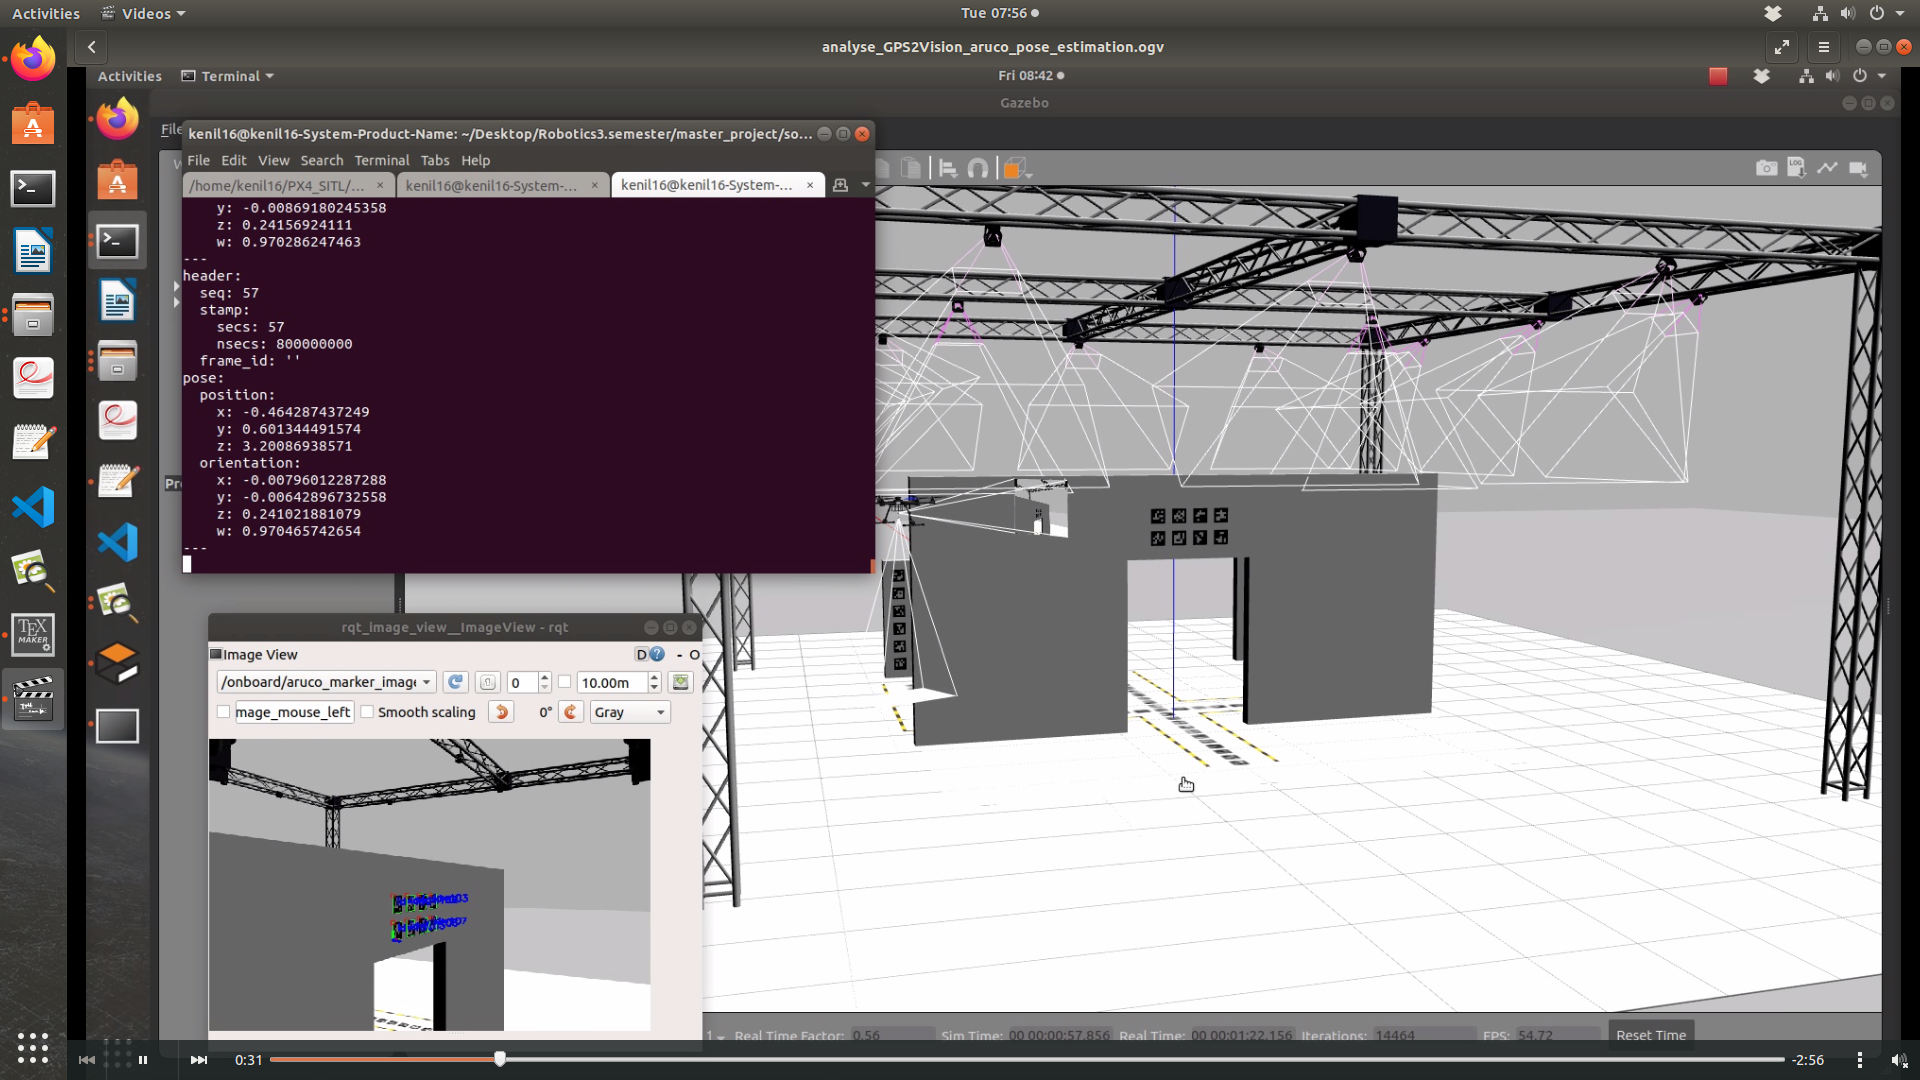
\includegraphics[width=\textwidth]{../Figures/GPS2Vision_pose_estimation_test/gps2vision_pose_estimation_one.png}
        \caption{}
        \label{fig:GPS2Vision_pose_estimation_one}
    \end{subfigure}
    \hspace{0.2em}
    \begin{subfigure}[t]{.30\textwidth}
        \centering
        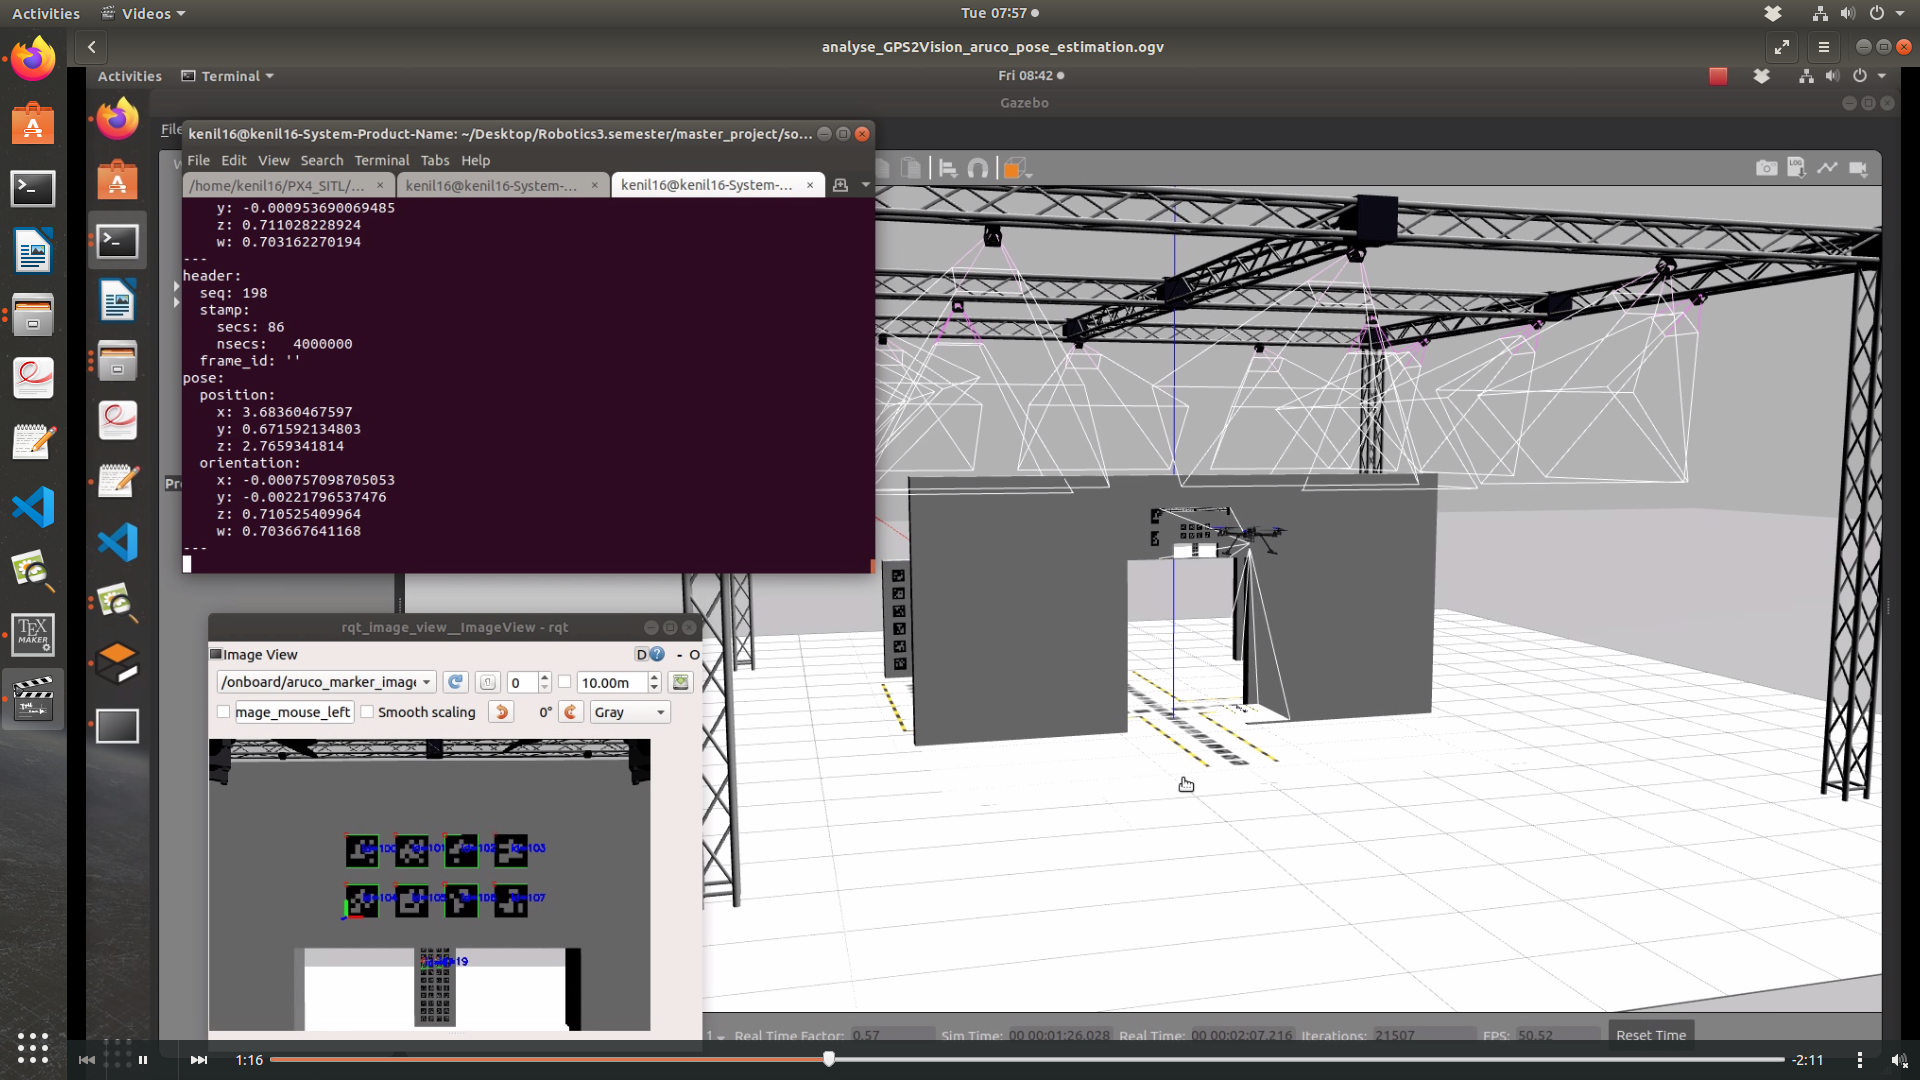
\includegraphics[width=\textwidth]{../Figures/GPS2Vision_pose_estimation_test/gps2vision_pose_estimation_two.png}
        \caption{}
        \label{fig:GPS2Vision_pose_estimation_two}
    \end{subfigure}
        \hspace{0.2em}
    \begin{subfigure}[t]{.30\textwidth}
        \centering
        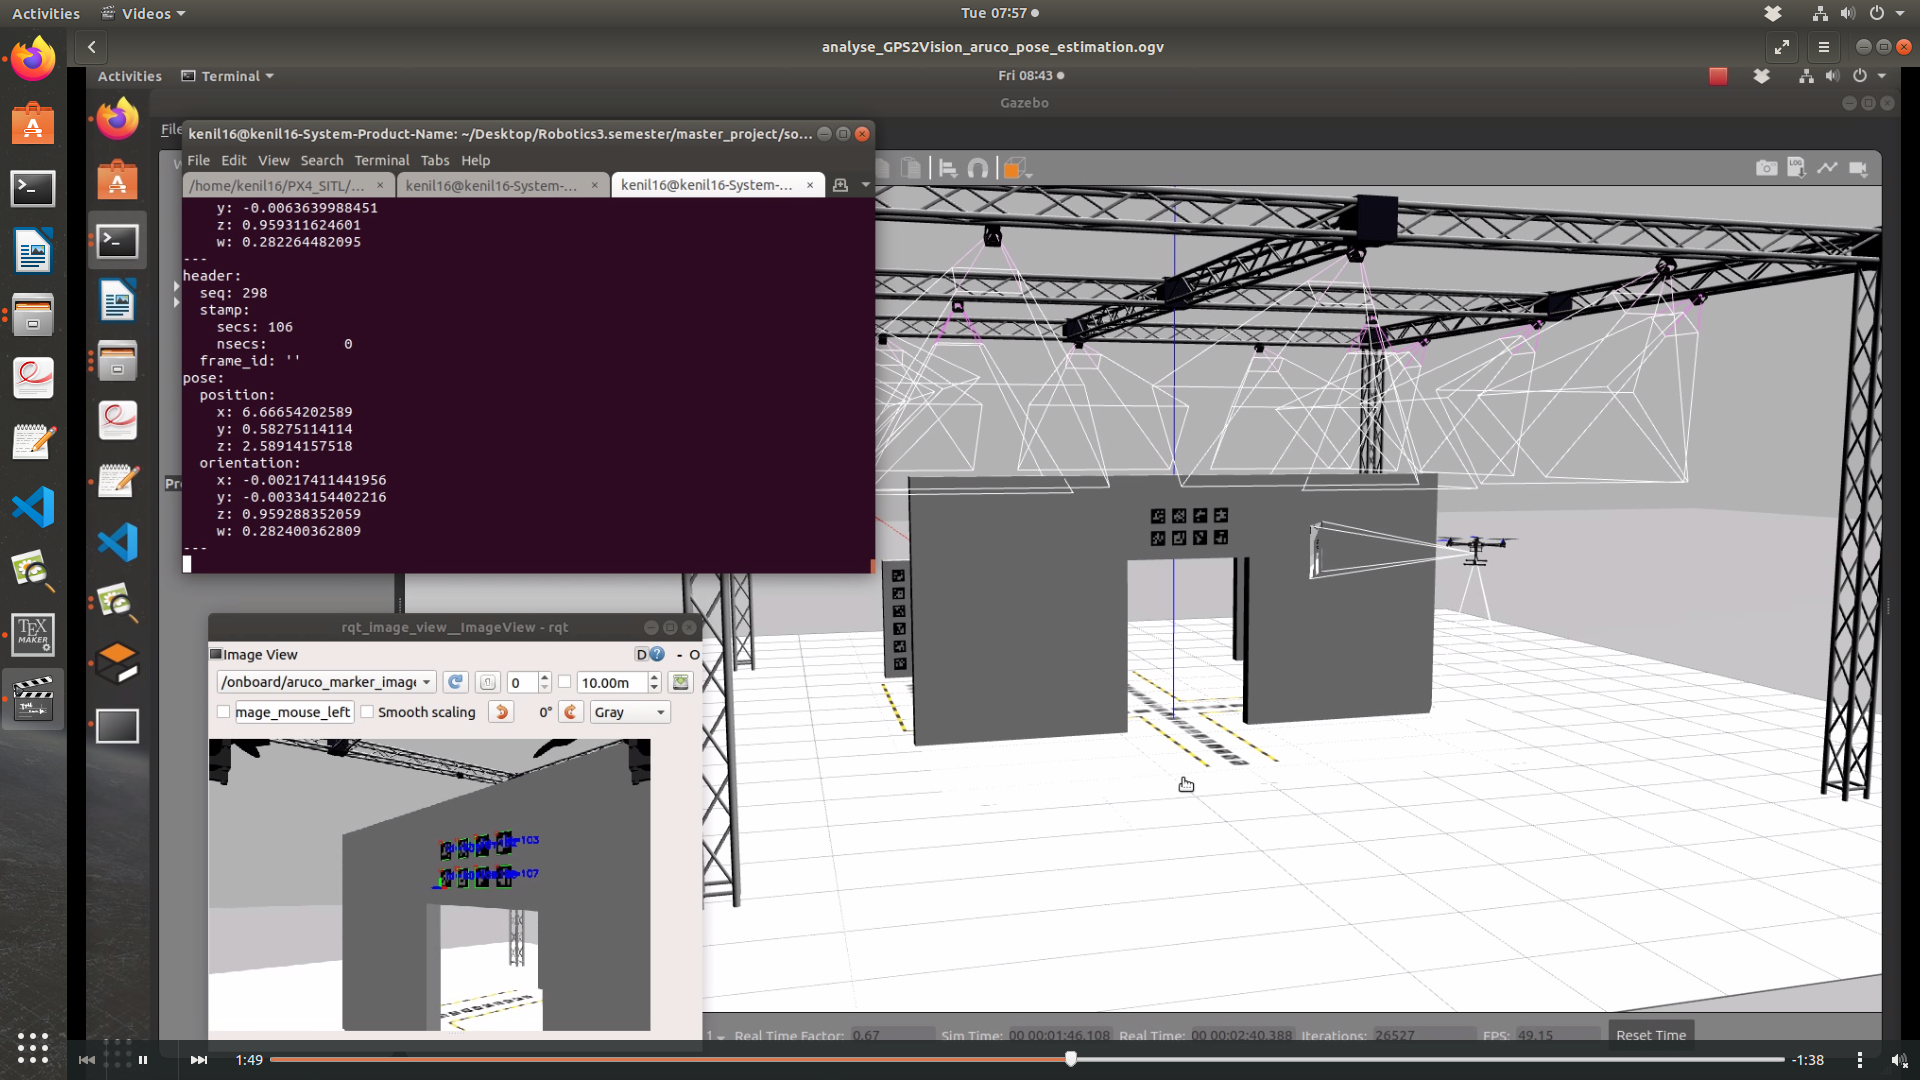
\includegraphics[width=\textwidth]{../Figures/GPS2Vision_pose_estimation_test/gps2vision_pose_estimation_three.png}
        \caption{}
        \label{fig:GPS2Vision_pose_estimation_three}
    \end{subfigure}
    \caption{Illustrations of the GPS2Vision pose estimation test in three different positions with the drone facing the GPS2Vision board. A video of the first couple of iterations can be seen on GitHub using \href{https://github.com/Kenil16/master_project/tree/master/test_videos/analyse_GPS2Vision_aruco_pose_estimation}{GPS2Vision pose estimation}
 }
    \label{fig:GPS2Vision_pose_estimation}
\end{figure}

The errors can be seen to be high when the drone is approximately 5-8 meters away from the GPS2Vision board which goes for both position and angle. From these observations, a \textit{safe area} for the transition between using GPS to vision as navigation would be within a radius of approximately five meters away from the GPS2Vision board which can be seen in Figure \ref{fig:GPS2Vision_pose_estimation_test1_error_pos} and \ref{fig:GPS2Vision_pose_estimation_test1_error_ori}. A possible reason why especially the z position deviates a lot when moving away from the board is that the z component in the coordinate system moves with an angle in roll which triggers the altitude of the drones to go from positive to negative and hence increases the error in z more than x and y which are less sensitive according to the analysis. 

\begin{figure}[H]
    \centering
    \begin{subfigure}[t]{.337\textwidth}
        \centering
        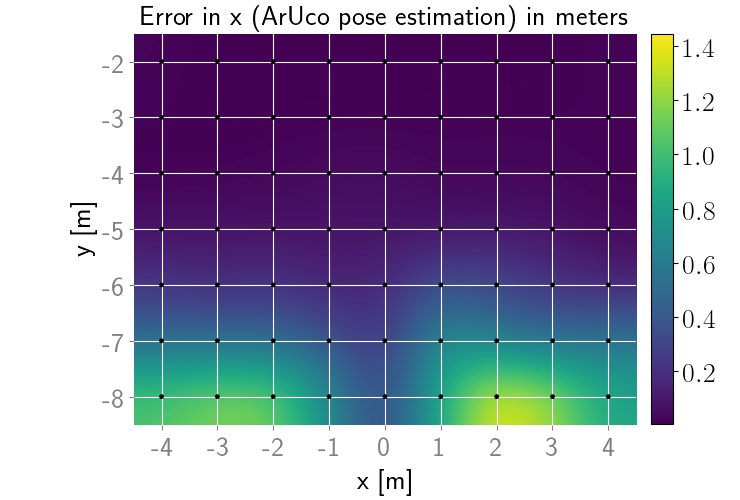
\includegraphics[width=\textwidth]{../Figures/GPS2Vision_pose_estimation_test/test1_aruco_board_width_0.2_space_0.1/aruco_pose_estimation_error_x.png}
        \caption{}
        \label{fig:GPS2Vision_pose_estimation_test1_error_x}
    \end{subfigure}
    \hspace{-0.9em}
    \begin{subfigure}[t]{.337\textwidth}
        \centering
        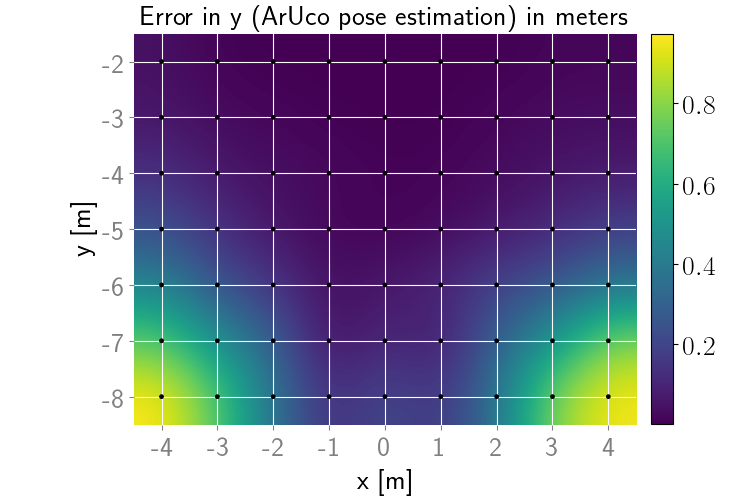
\includegraphics[width=\textwidth]{../Figures/GPS2Vision_pose_estimation_test/test1_aruco_board_width_0.2_space_0.1/aruco_pose_estimation_error_y.png}
        \caption{}
        \label{fig:GPS2Vision_pose_estimation_test1_error_y}
    \end{subfigure}
    \hspace{-0.9em}
    \begin{subfigure}[t]{.337\textwidth}
        \centering
        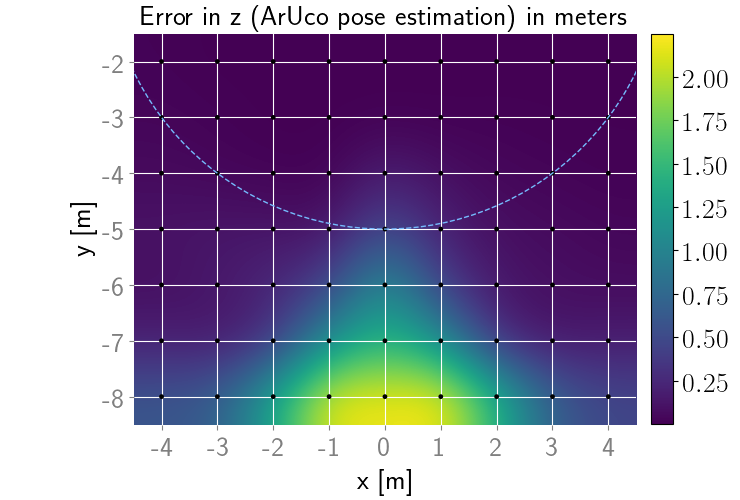
\includegraphics[width=\textwidth]{../Figures/GPS2Vision_pose_estimation_test/test1_aruco_board_width_0.2_space_0.1/aruco_pose_estimation_error_z.png}
        \caption{}
        \label{fig:GPS2Vision_pose_estimation_test1_error_z}
    \end{subfigure}
    \caption{Black dots indicates where the drone has estimated the pose of the ArUco board and the circle colored sky blue indicates a safe GPS2Vision transition area. It may the noticed that the error in the position estimate becomes quite high when the drone has a distance of 7-8 meters away from the GPS2Vision board}
    \label{fig:GPS2Vision_pose_estimation_test1_error_pos}
\end{figure}

\begin{figure}[H]
    \centering
    \begin{subfigure}[t]{.337\textwidth}
        \centering
        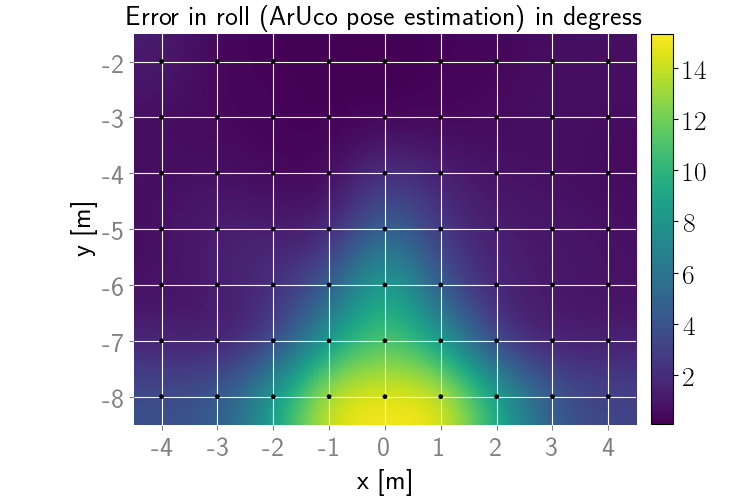
\includegraphics[width=\textwidth]{../Figures/GPS2Vision_pose_estimation_test/test1_aruco_board_width_0.2_space_0.1/aruco_pose_estimation_error_roll.png}
        \caption{}
        \label{fig:GPS2Vision_pose_estimation_test1_error_roll}
    \end{subfigure}
    \hspace{-0.9em}
    \begin{subfigure}[t]{.337\textwidth}
        \centering
        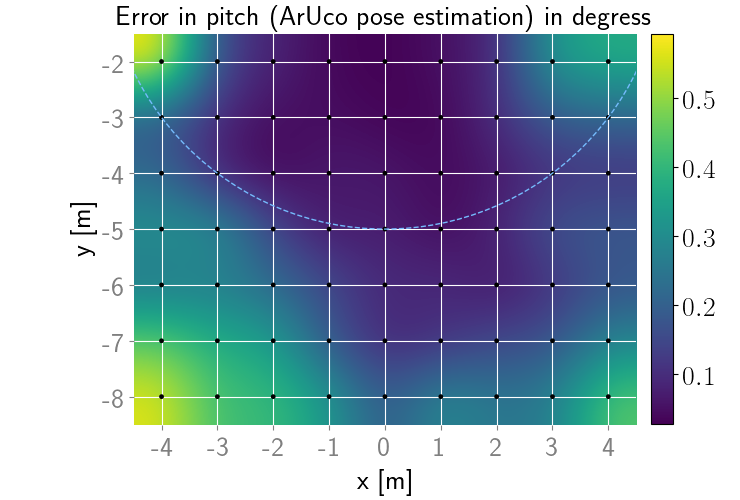
\includegraphics[width=\textwidth]{../Figures/GPS2Vision_pose_estimation_test/test1_aruco_board_width_0.2_space_0.1/aruco_pose_estimation_error_pitch.png}
        \caption{}
        \label{fig:GPS2Vision_pose_estimation_test1_error_pitch}
    \end{subfigure}
    \hspace{-0.9em}
    \begin{subfigure}[t]{.337\textwidth}
        \centering
        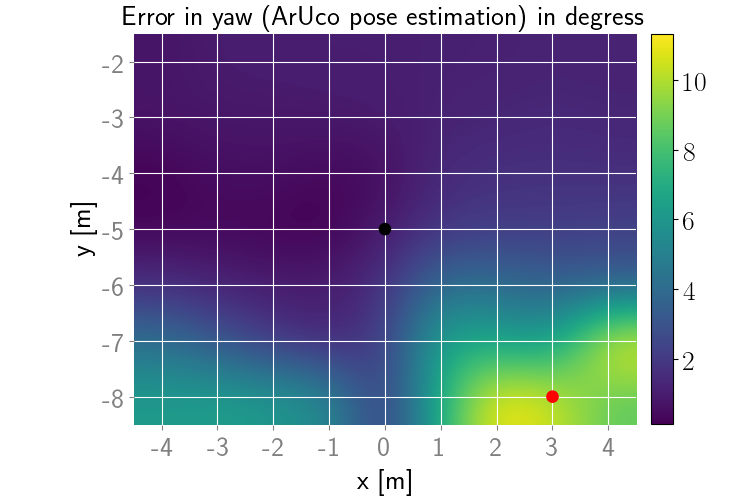
\includegraphics[width=\textwidth]{../Figures/GPS2Vision_pose_estimation_test/test1_aruco_board_width_0.2_space_0.1/aruco_pose_estimation_error_yaw.png}
        \caption{}
        \label{fig:GPS2Vision_pose_estimation_test1_error_yaw}
    \end{subfigure}
    \caption{Black dots indicates where the drone has estimated the pose of the ArUco board and the circle colored sky blue indicates a safe GPS2Vision transition area. It may the noticed that the error in the angle estimate becomes quite high when the drone has a distance of 7-8 meters away from the GPS2Vision board}
    \label{fig:GPS2Vision_pose_estimation_test1_error_ori}
\end{figure}

Based on the results, the maximum distance away from the GPS2Vision board when executing the GPS to vision transition will be 5 meters which will be used in the implementation of the code.

\subsubsection{Rolling average from ArUco pose estimation}
\label{sec:rolling_average_aruco_pose_estimation}

To analyze the possibility of fluctuations in the ArUco pose estimates, the rolling average is used for calculating the mean and standard deviation (STD) in two different positions for one-hundred iterations. This can be seen in Figure \ref{fig:rolling_average_pos}. 

\begin{figure}[H]
    \centering
    \begin{subfigure}[t]{.30\textwidth}
        \centering
        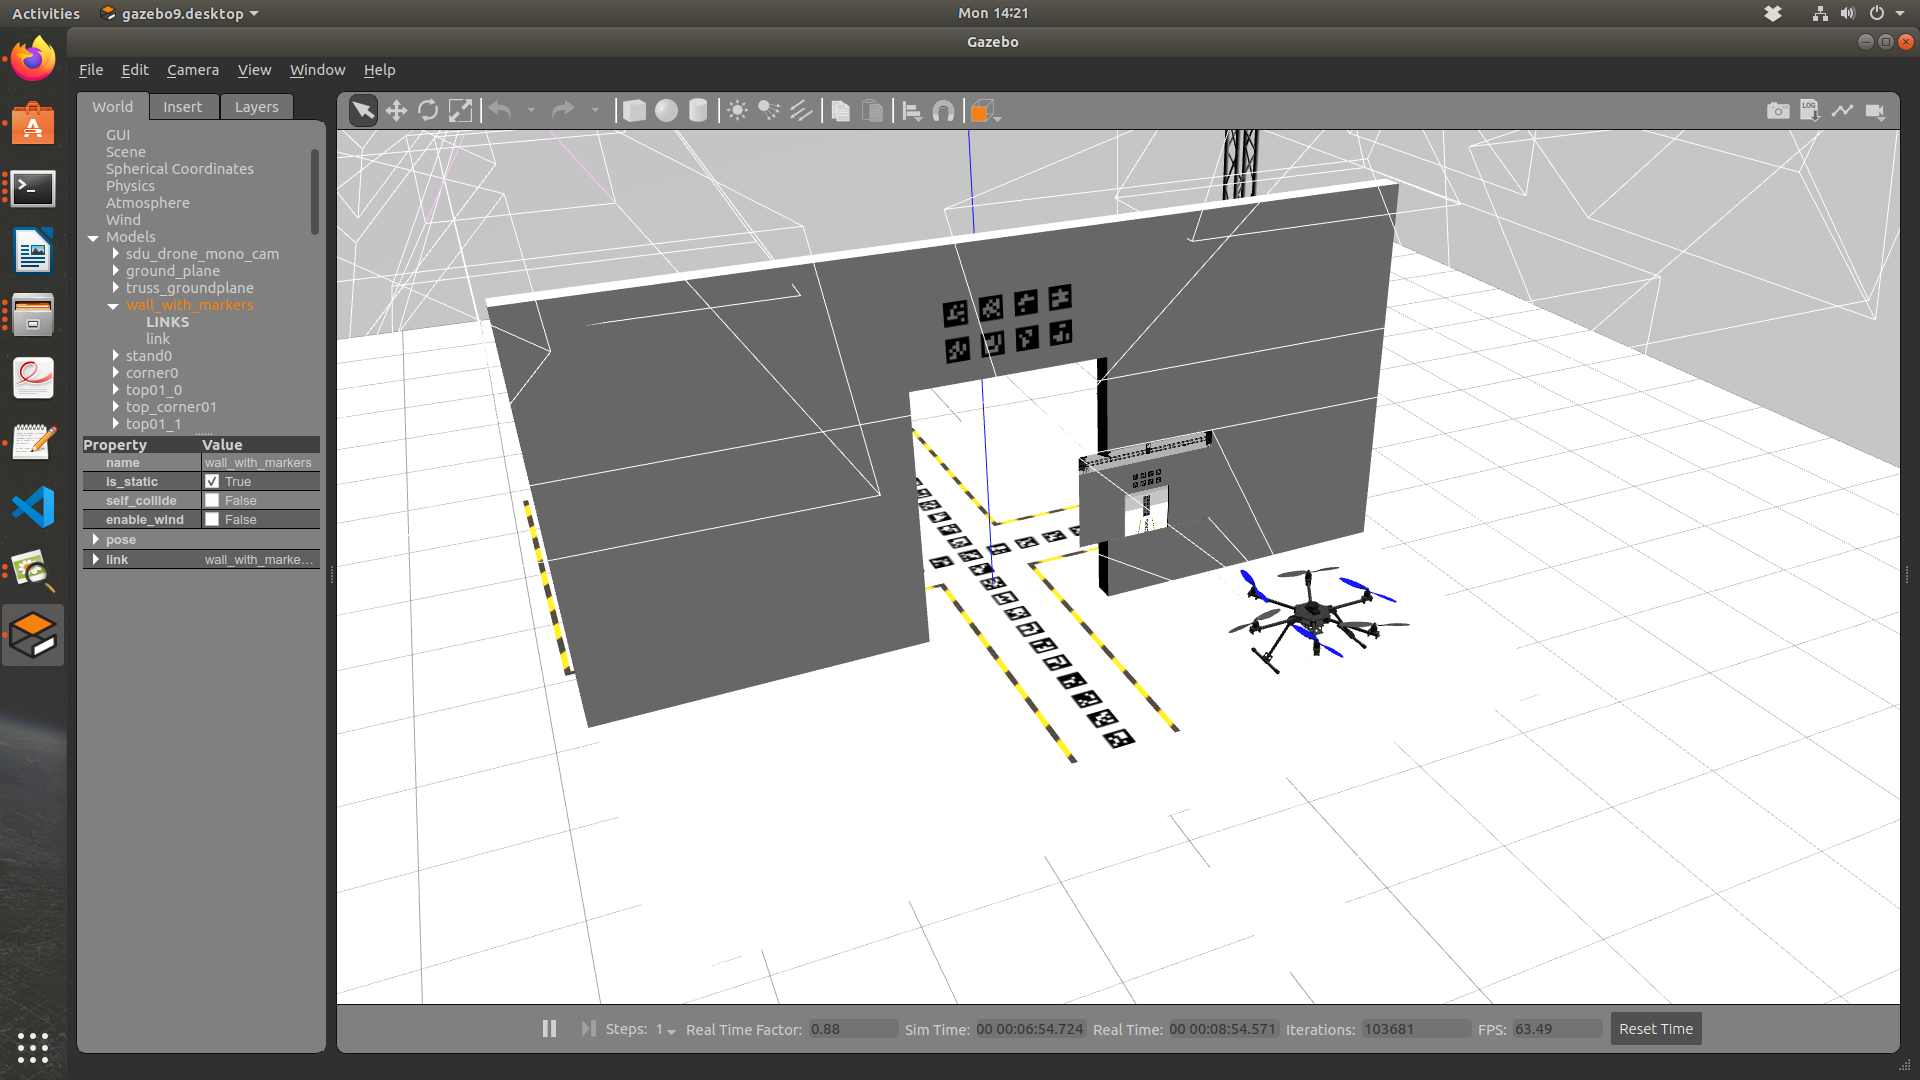
\includegraphics[width=\textwidth]{../Figures/analyse_rolling_average/optimal_pose.png}
        \caption{}
        \label{fig:rolling_average_good_pos}
    \end{subfigure}
    \hspace{0.5em}
    \begin{subfigure}[t]{.30\textwidth}
        \centering
        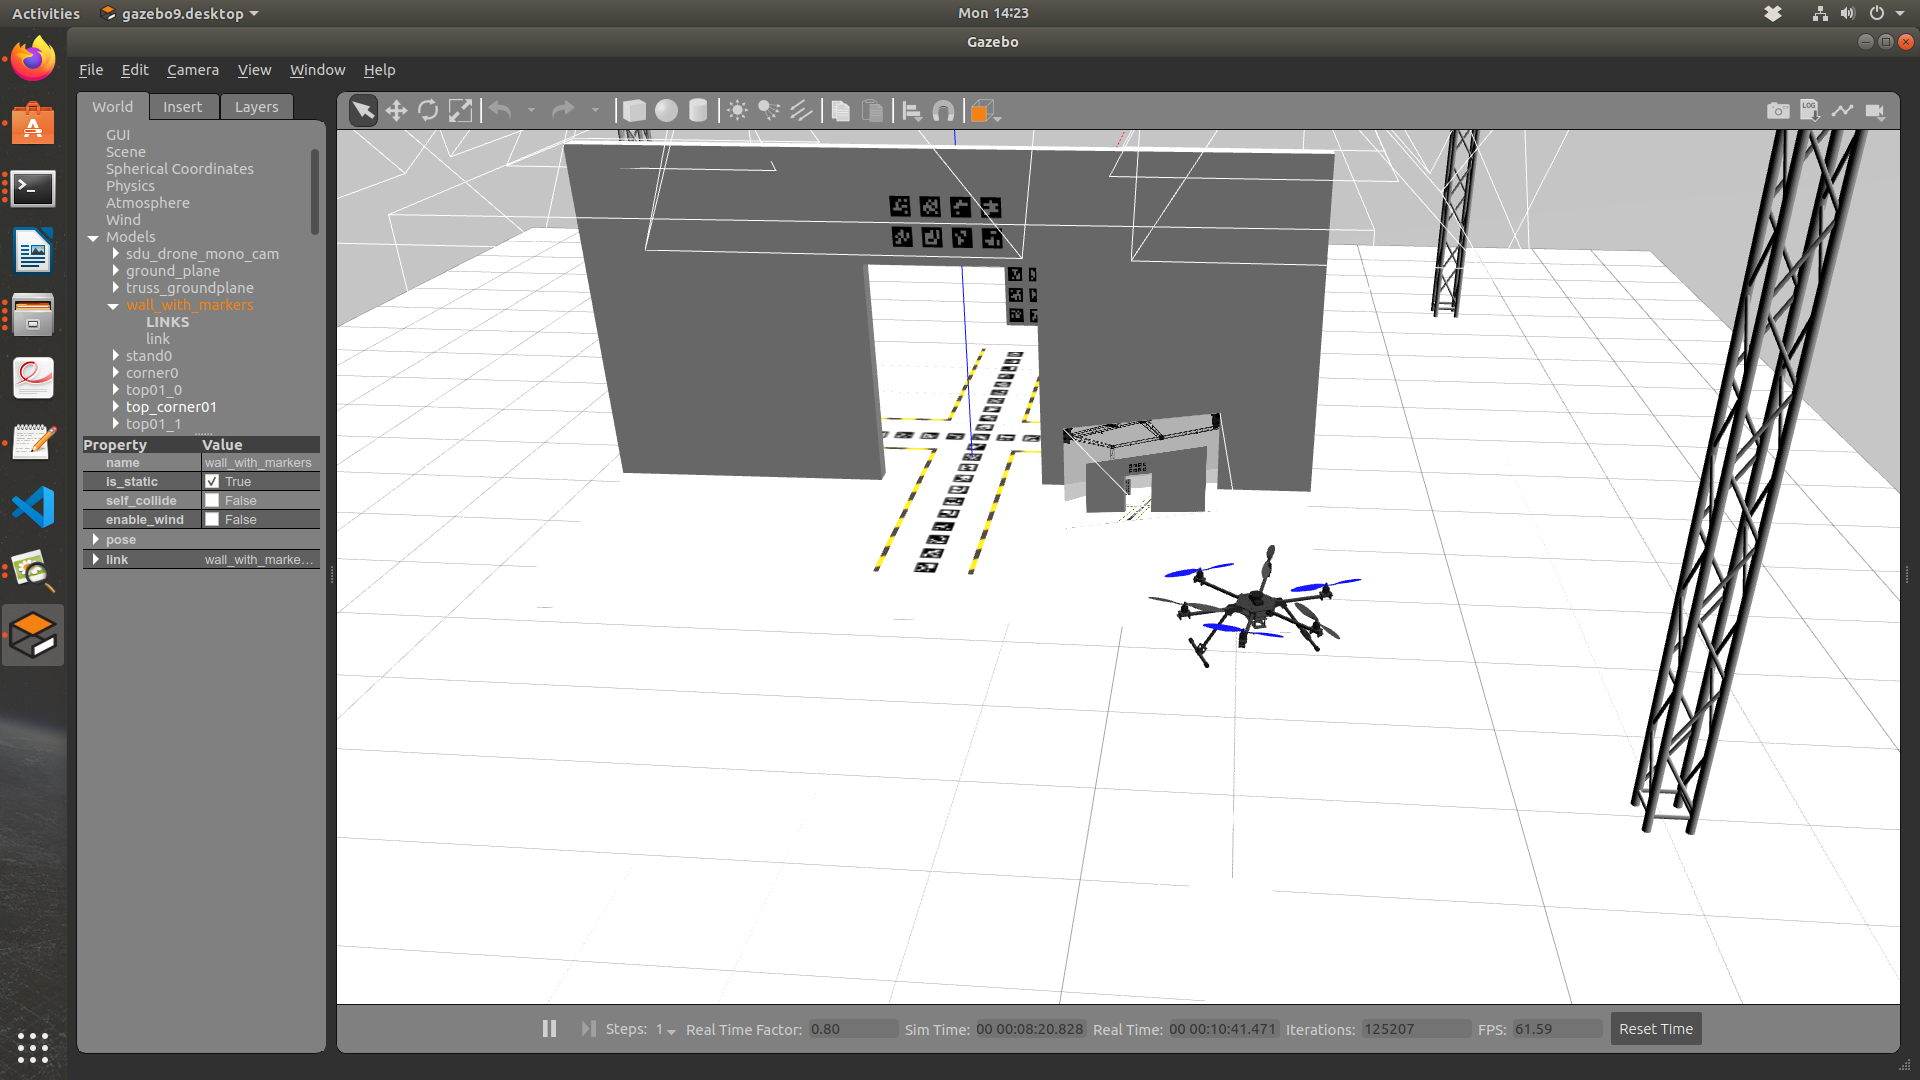
\includegraphics[width=\textwidth]{../Figures/analyse_rolling_average/bad_pose.png}
        \caption{}
        \label{fig:rolling_average_bad_pos}
    \end{subfigure}
    \caption{Illustrations of the two positions used to evaluate the rolling average for one-hundred iterations. The positions of the drone in Figures \ref{fig:rolling_average_good_pos} and \ref{fig:rolling_average_bad_pos} are (0,-5) and (3,-7) respectively from the coordinate system in Figures \ref{fig:GPS2Vision_pose_estimation_test1_error_pos} and \ref{fig:GPS2Vision_pose_estimation_test1_error_ori}} 
    \label{fig:rolling_average_pos}
\end{figure}

This is done as an extension to the maximum allowed distance from the GPS2Vision marker from Section \ref{sec:GPS2Vision_pose_estimation} to insure that the GPS to vision transition is only performed when the pose estimates are stable and reliable. 

\begin{figure}[H]
    \centering
    \begin{subfigure}[t]{.30\textwidth}
        \centering
        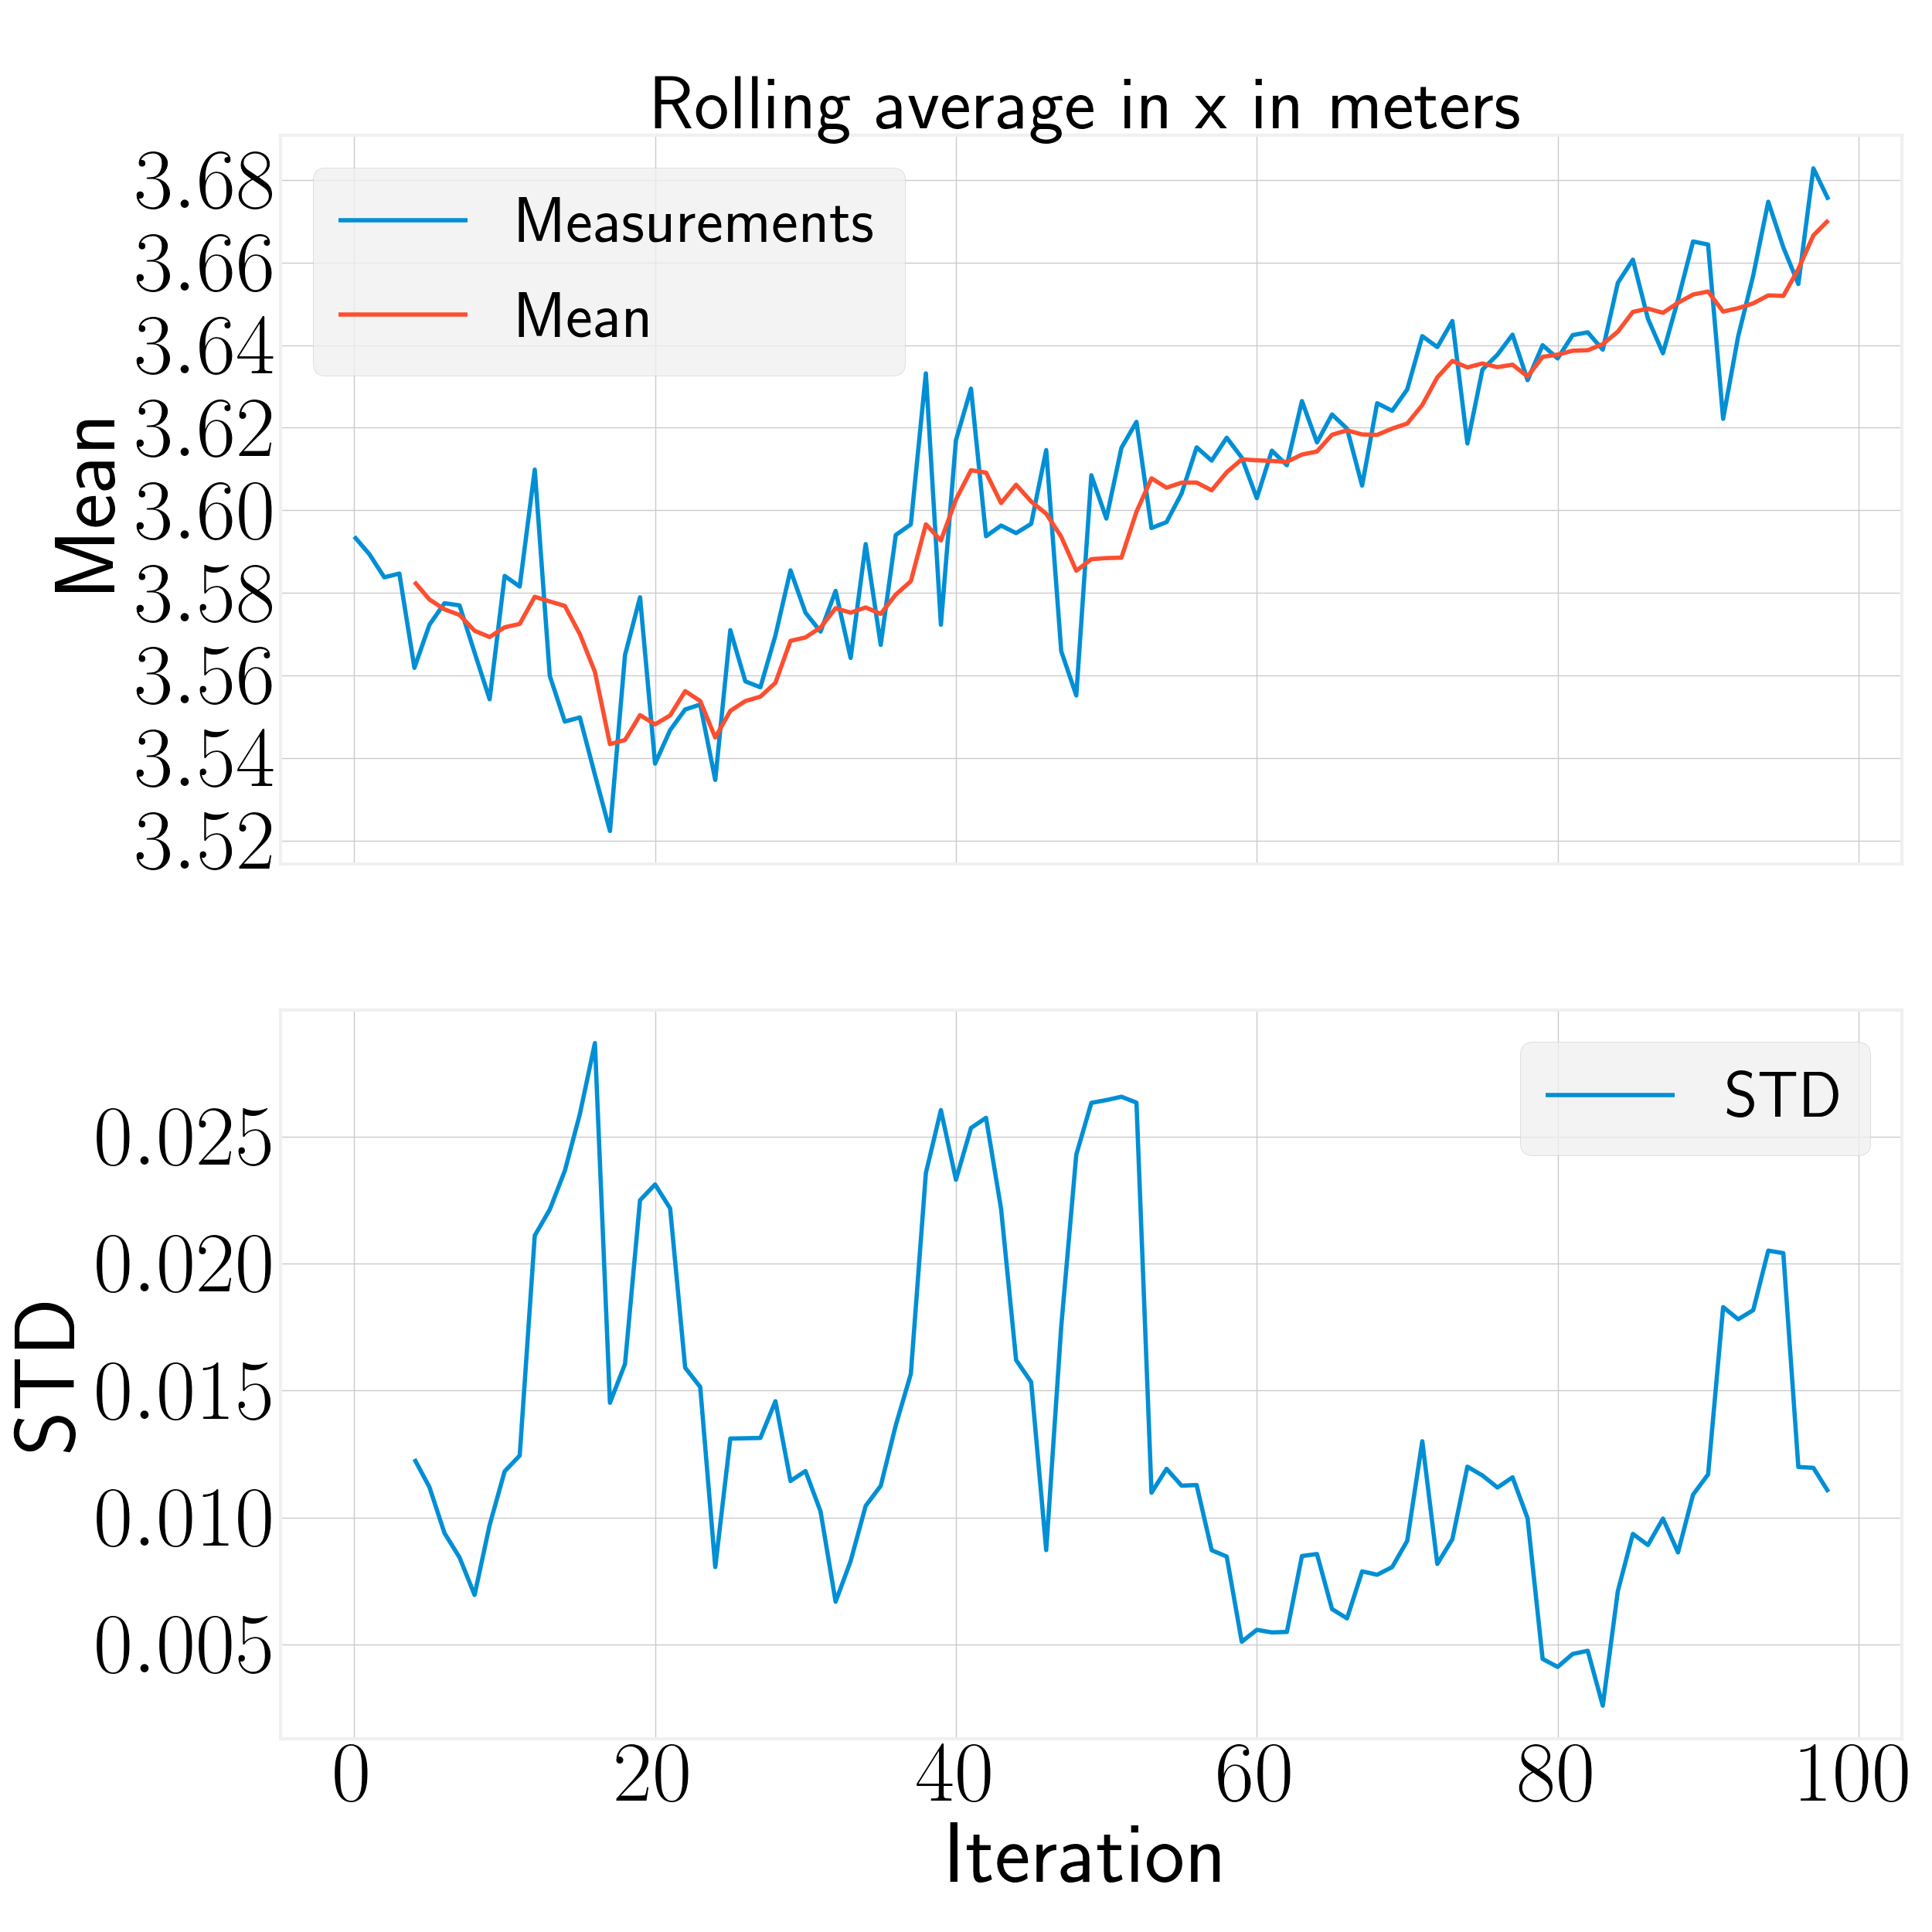
\includegraphics[width=\textwidth]{../Figures/analyse_rolling_average/test1/Calculated_rolling_average_in_x_with_mean_and_STD.png}
        \caption{}
        \label{fig:rolling_average_in_x_test1}
    \end{subfigure}
     \hspace{0.2em}
    \begin{subfigure}[t]{.30\textwidth}
        \centering
        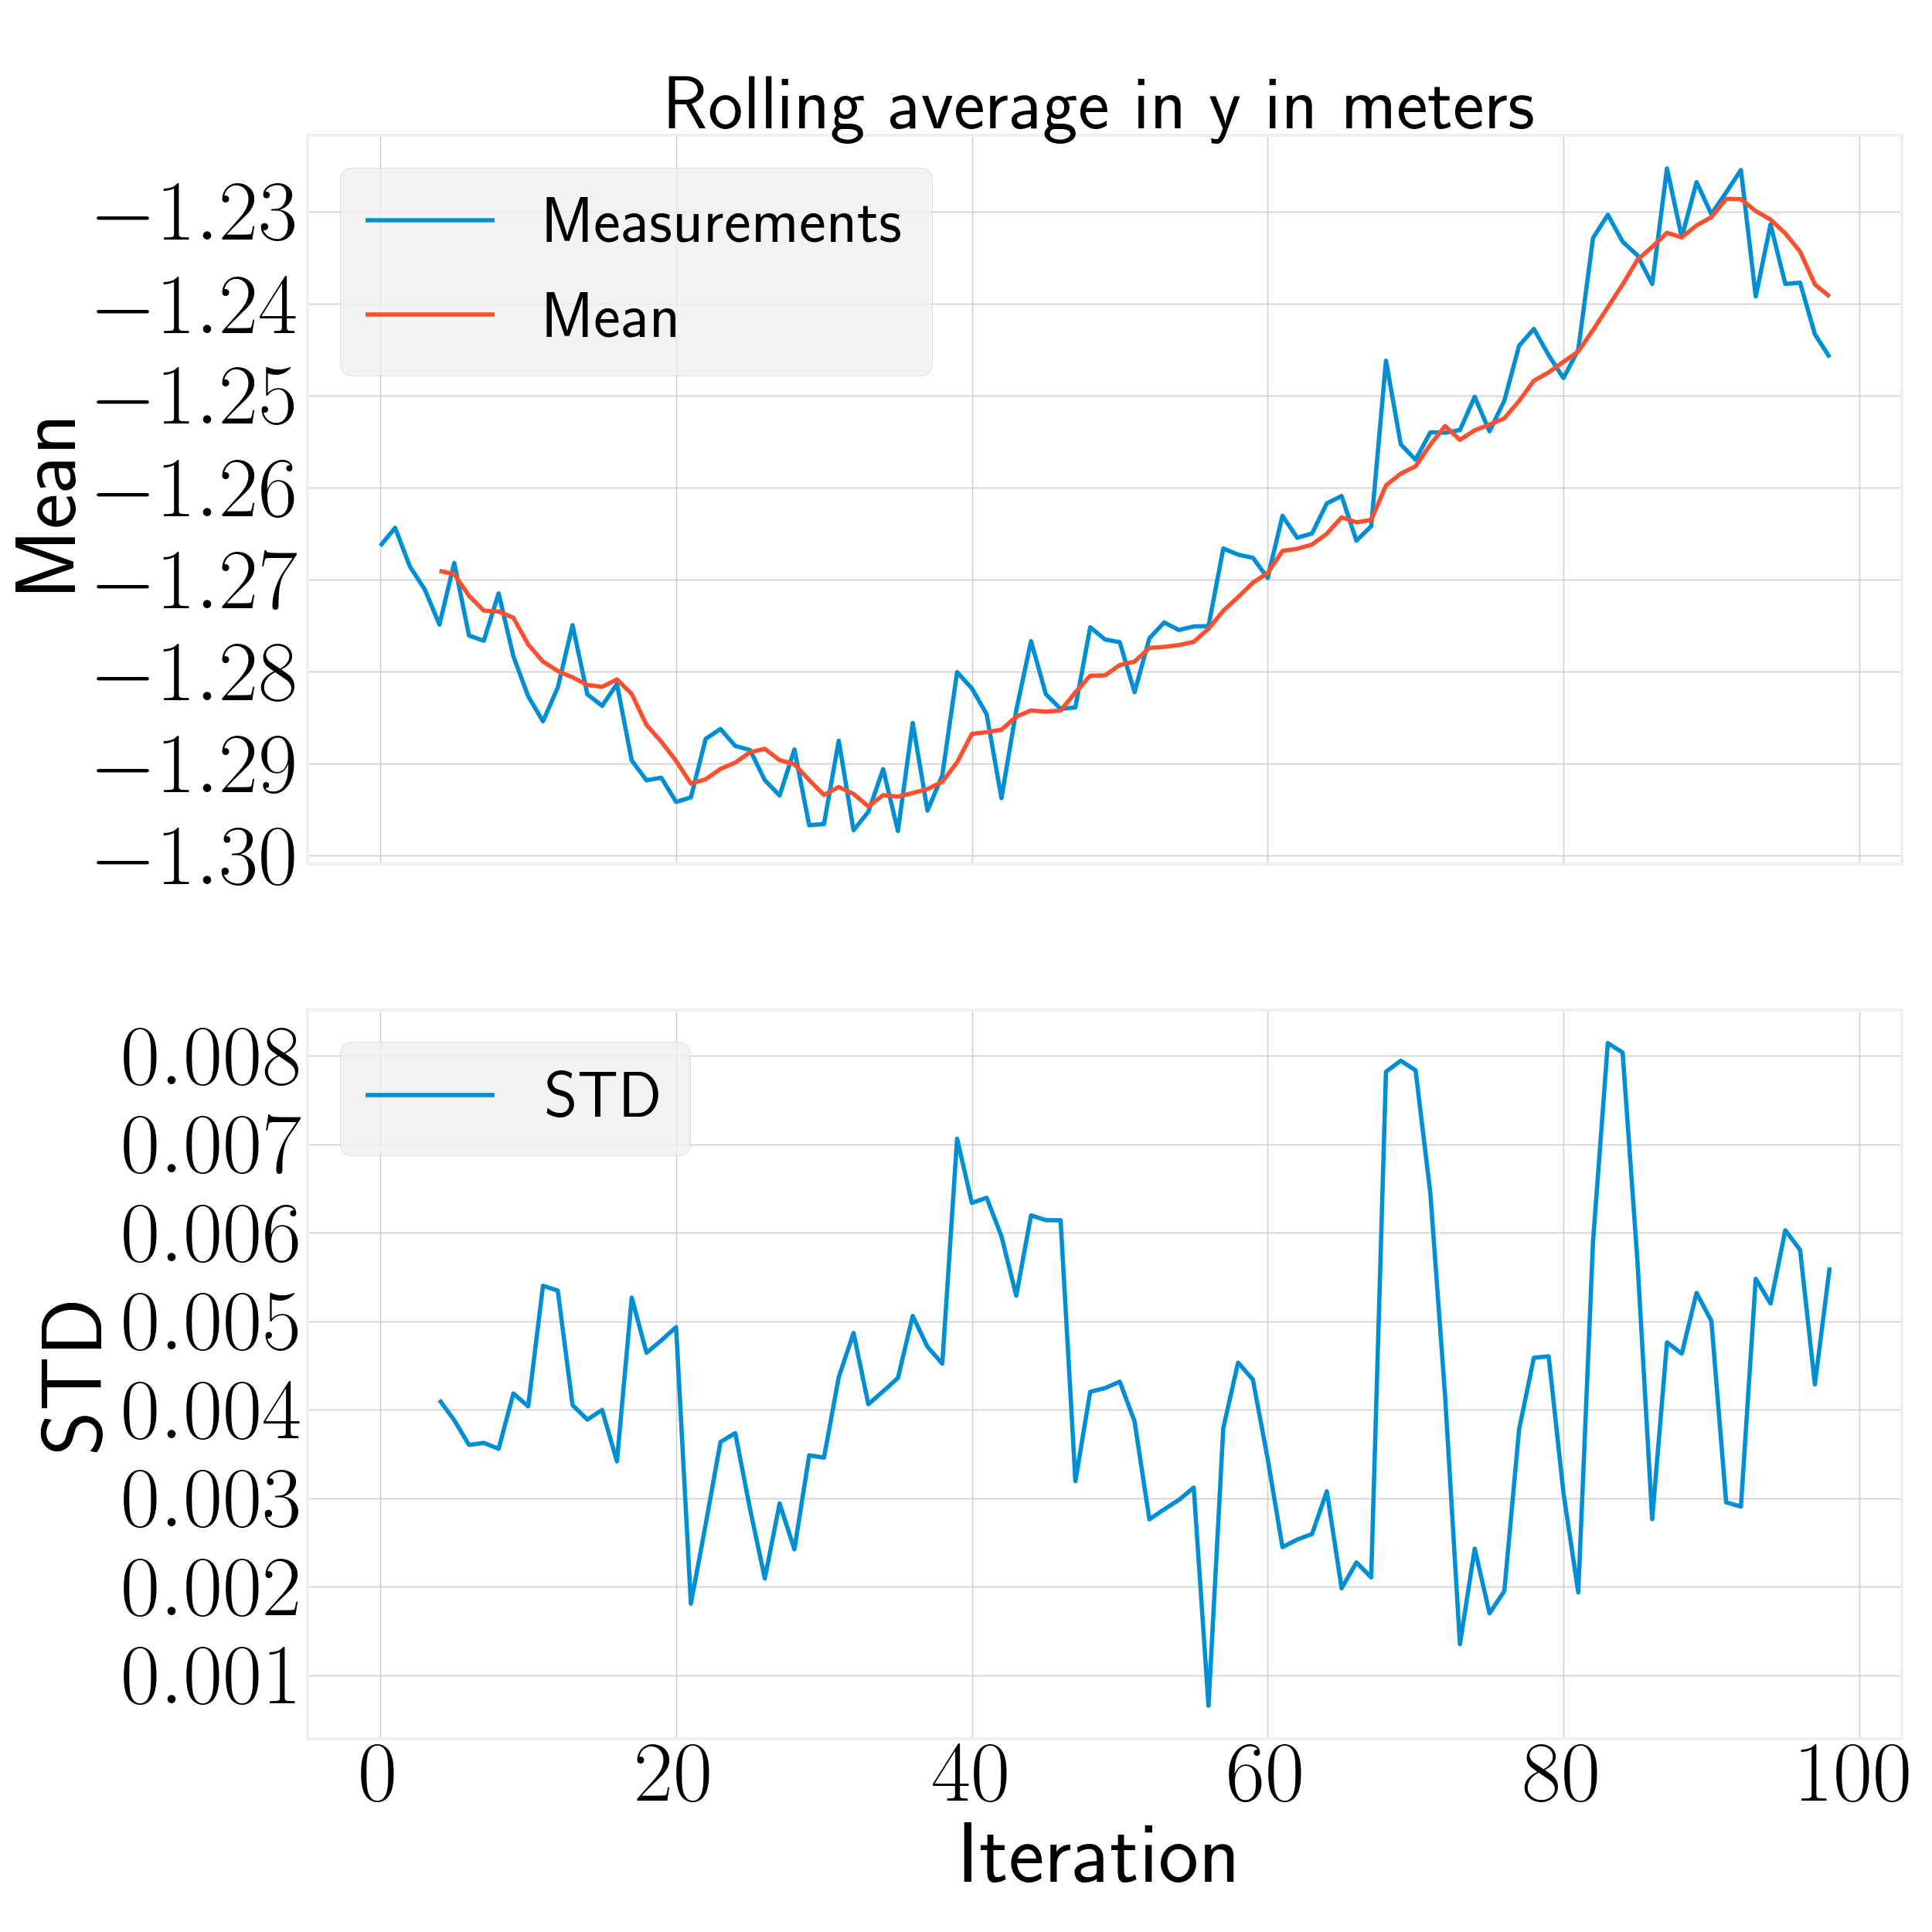
\includegraphics[width=\textwidth]{../Figures/analyse_rolling_average/test1/Calculated_rolling_average_in_y_with_mean_and_STD.png}
        \caption{}
        \label{fig:rolling_average_in_y_test1}
    \end{subfigure}
     \hspace{0.2em}
    \begin{subfigure}[t]{.30\textwidth}
        \centering
        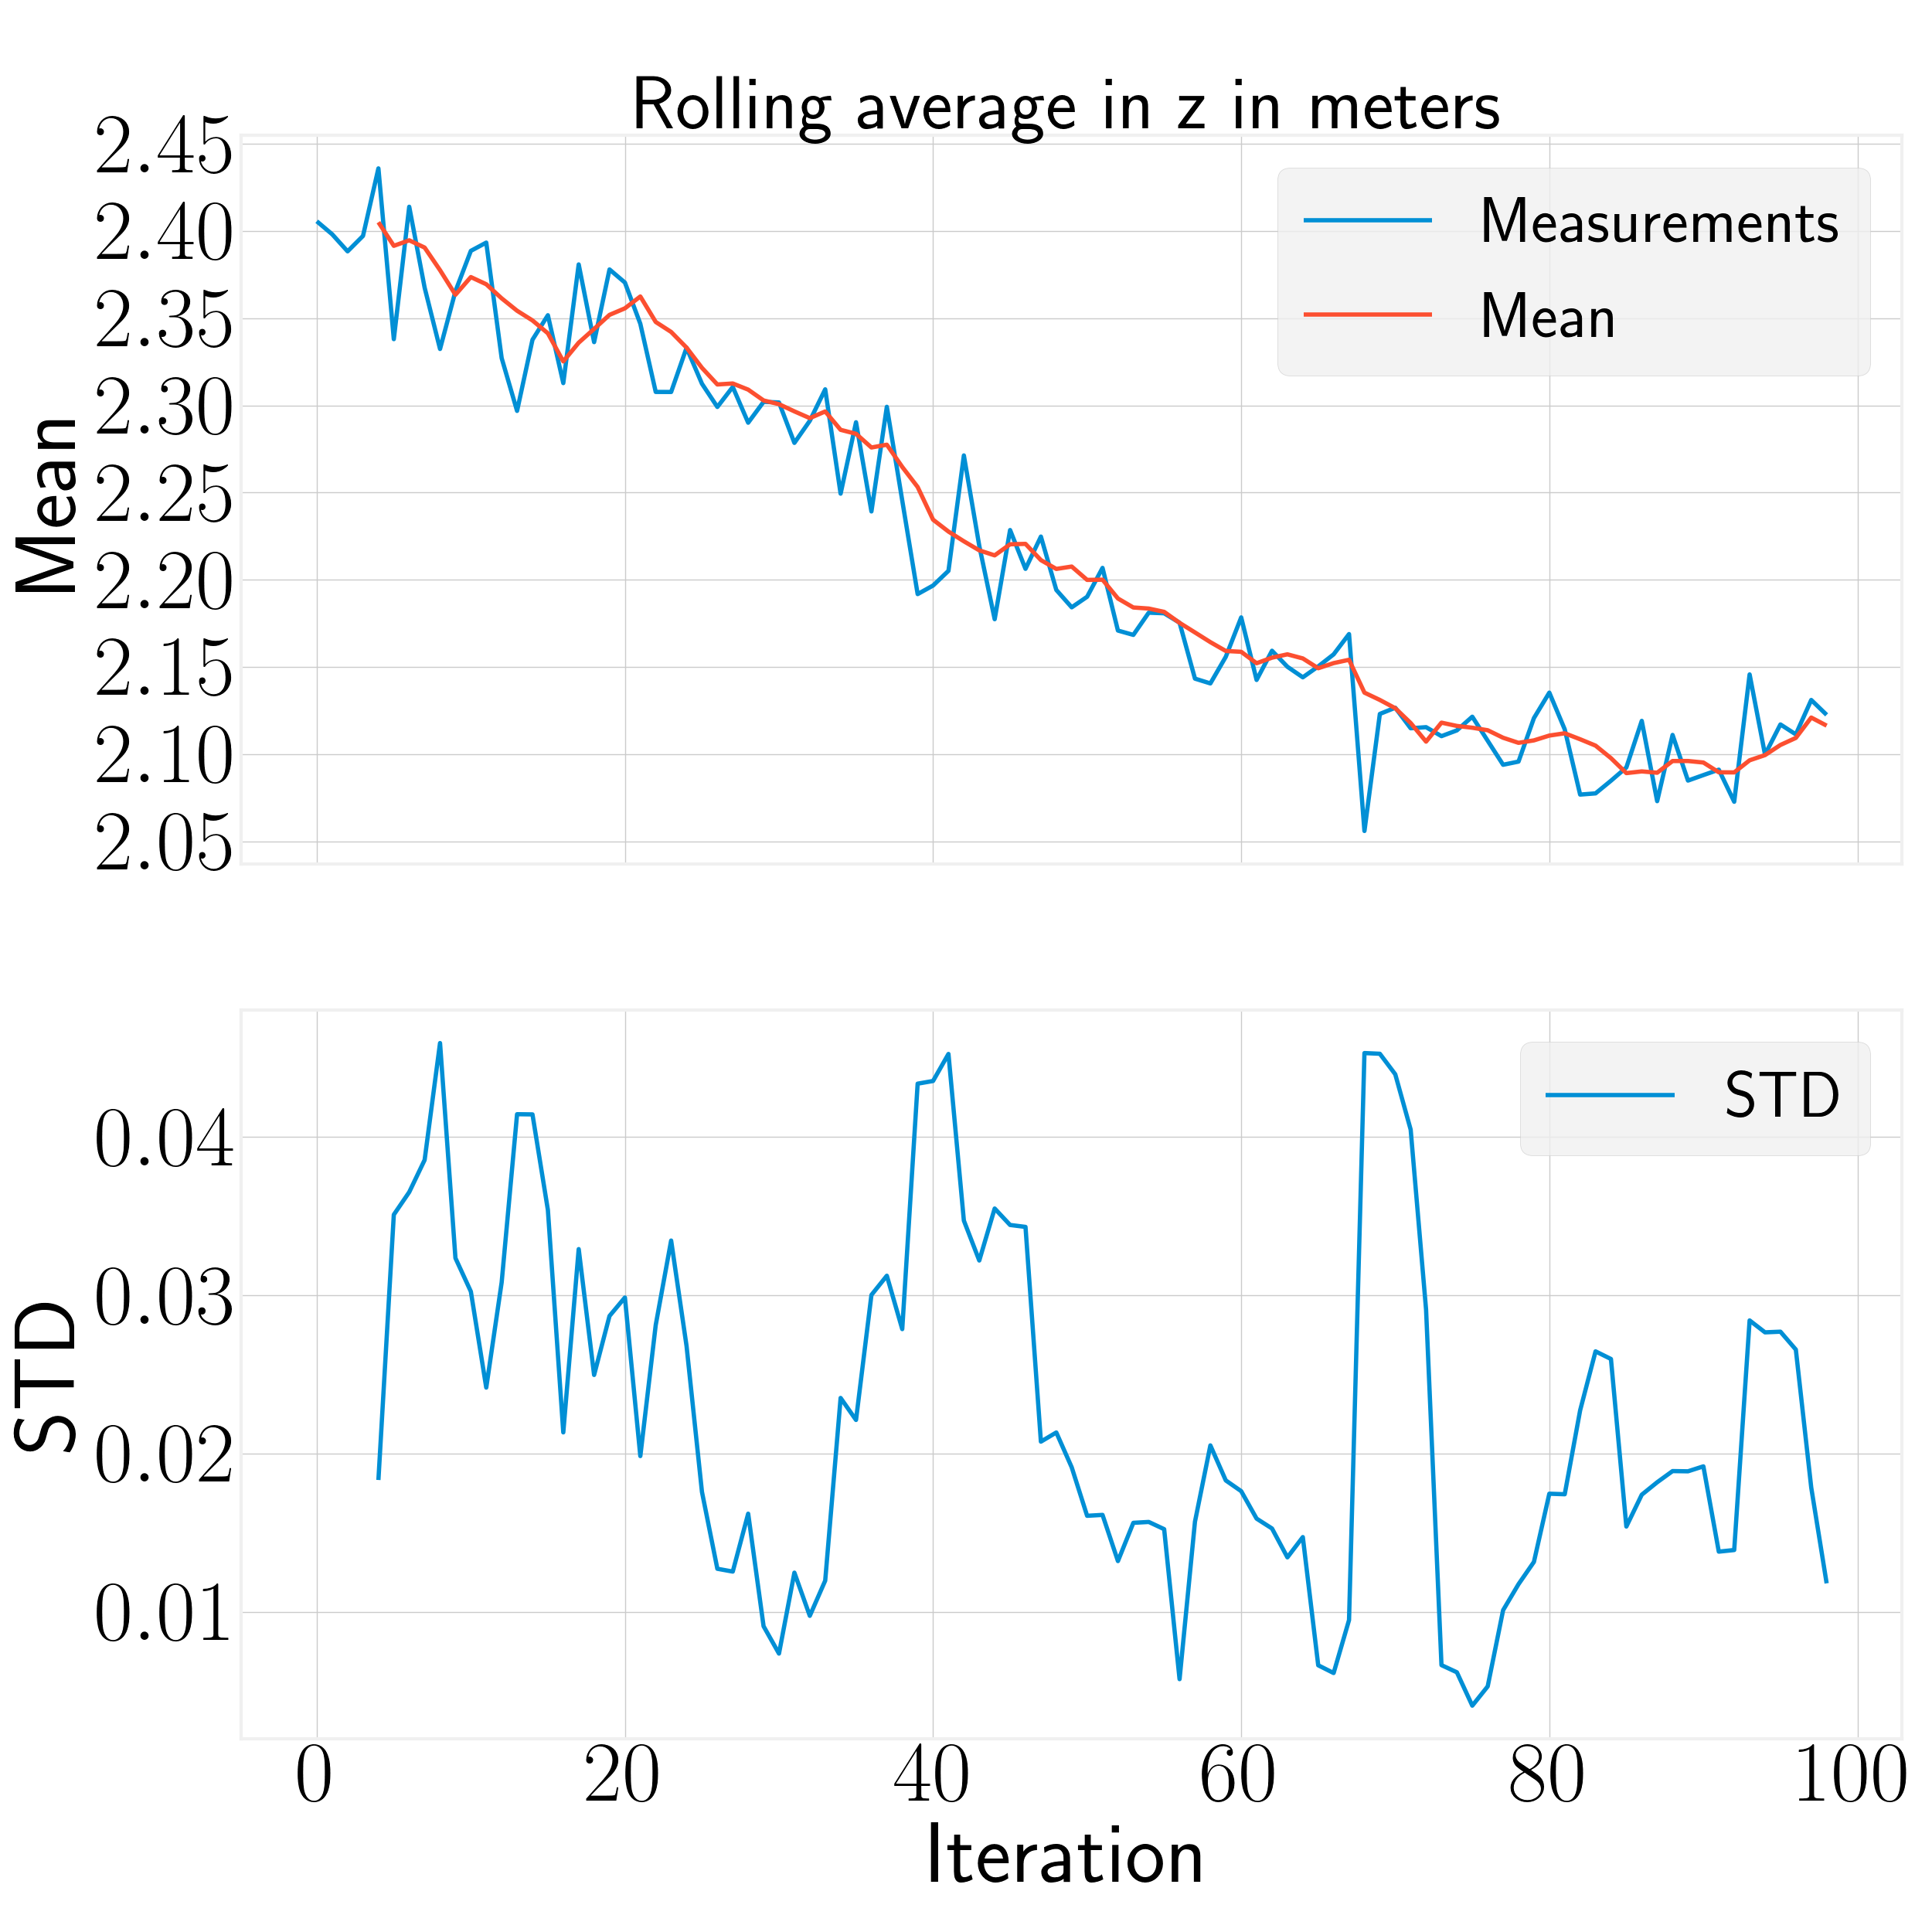
\includegraphics[width=\textwidth]{../Figures/analyse_rolling_average/test1/Calculated_rolling_average_in_z_with_mean_and_STD.png}
        \caption{}
        \label{fig:rolling_average_in_z_test1}
    \end{subfigure}
    \caption{Illustrations of the rolling average from the configuration in Figure \ref{fig:rolling_average_good_pos}. As it can be seen, the fluctuations of the position estimates are quite steady with only minor fluctuations of a few centimeters}
    \label{fig:rolling_average_pos_test1}
\end{figure}

\begin{figure}[H]
    \centering
    \begin{subfigure}[t]{.30\textwidth}
        \centering
        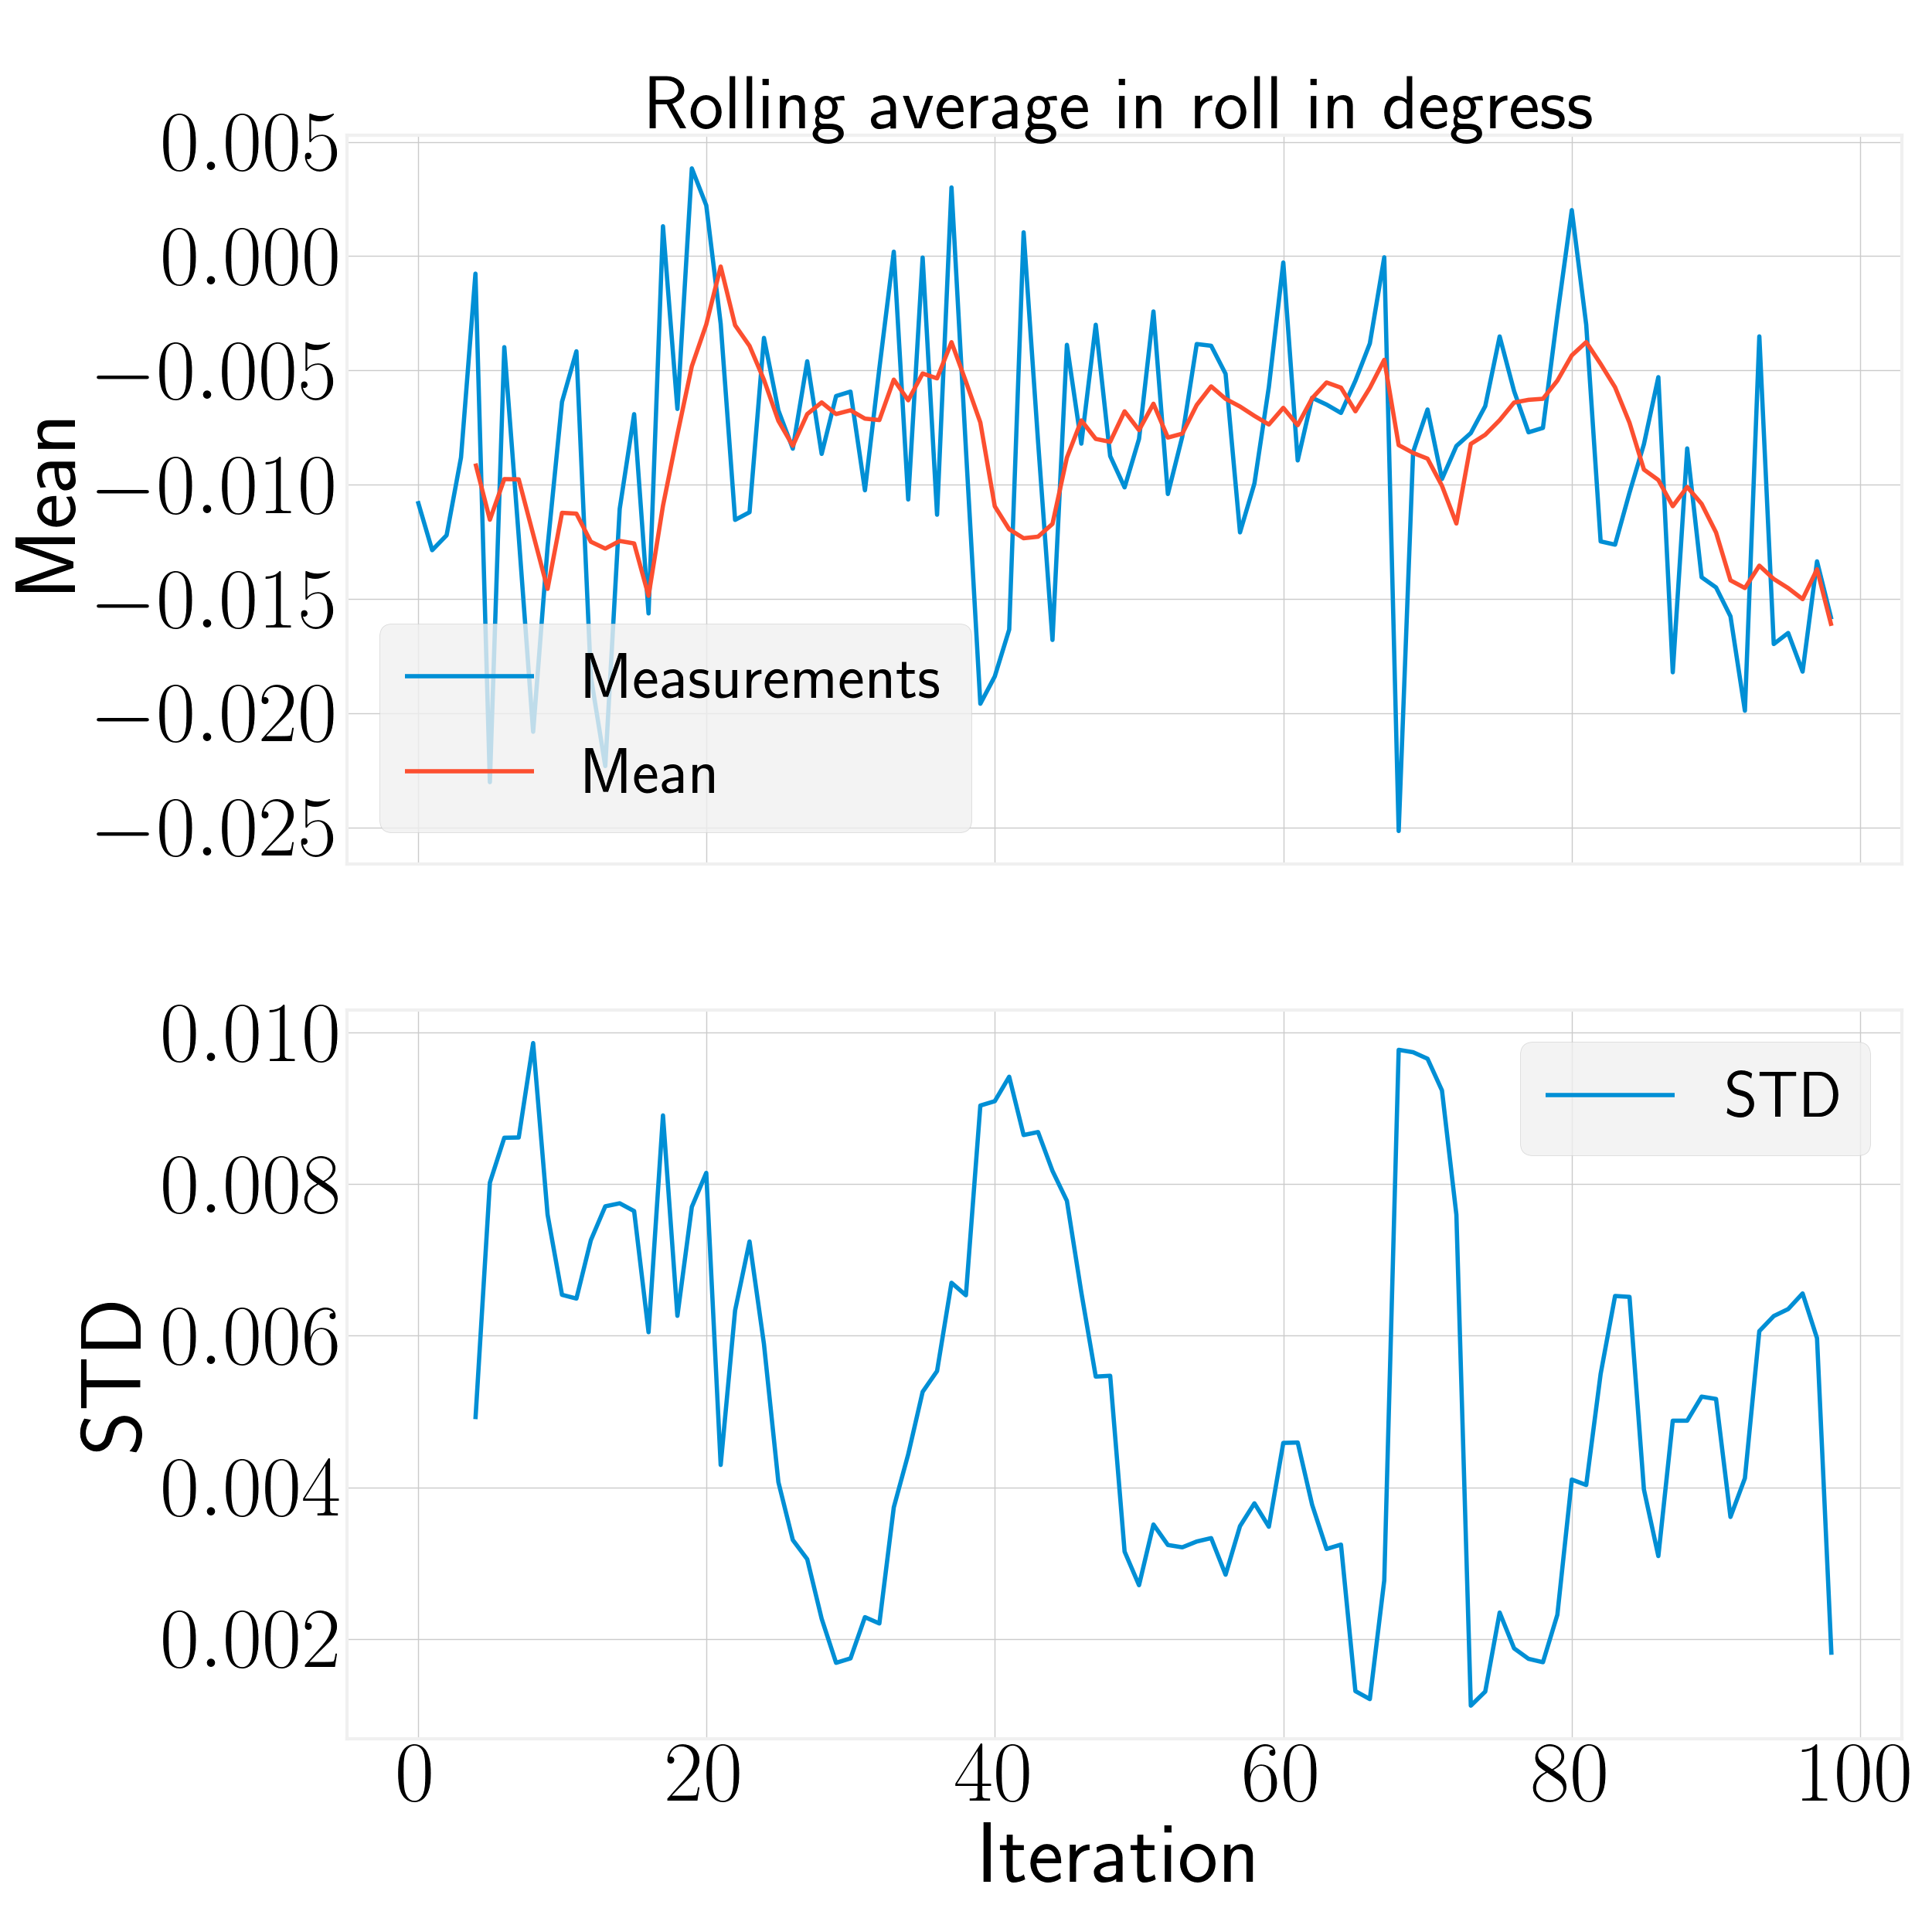
\includegraphics[width=\textwidth]{../Figures/analyse_rolling_average/test1/Calculated_rolling_average_in_roll_with_mean_and_STD.png}
        \caption{}
        \label{fig:rolling_average_in_roll_test1}
    \end{subfigure}
     \hspace{0.2em}
    \begin{subfigure}[t]{.30\textwidth}
        \centering
        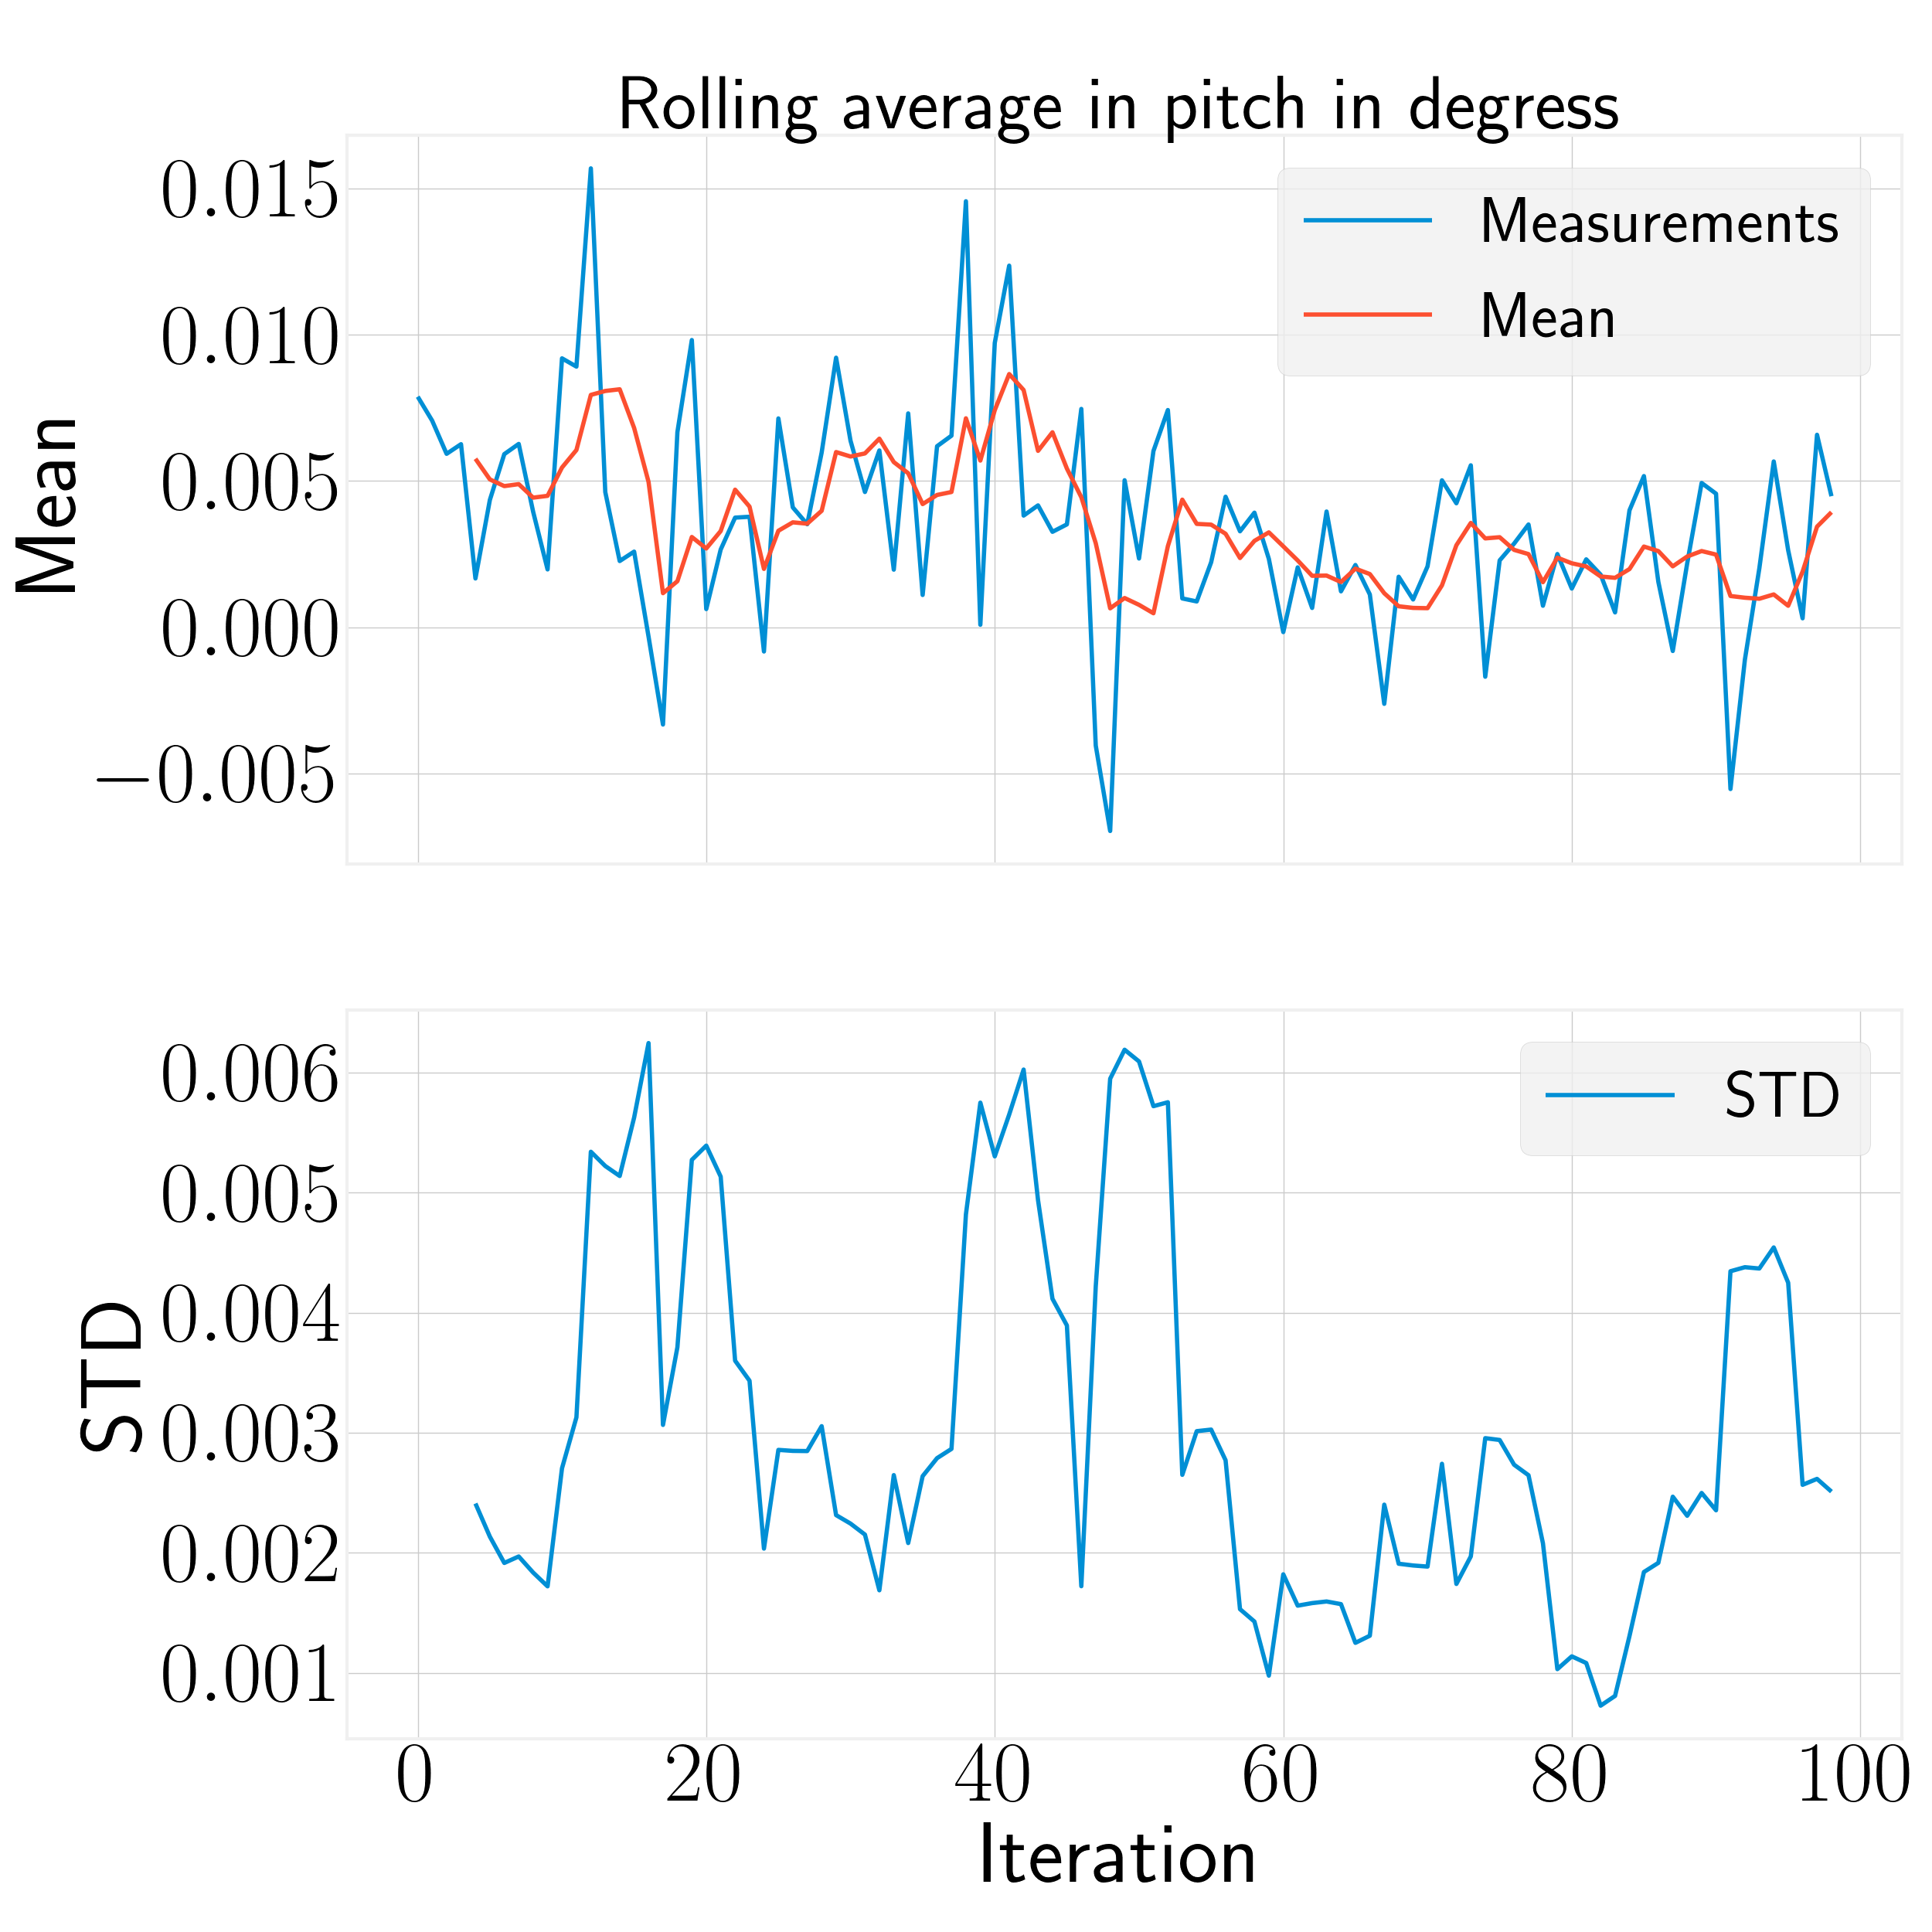
\includegraphics[width=\textwidth]{../Figures/analyse_rolling_average/test1/Calculated_rolling_average_in_pitch_with_mean_and_STD.png}
        \caption{}
        \label{fig:rolling_average_in_pitch_test1}
    \end{subfigure}
     \hspace{0.2em}
    \begin{subfigure}[t]{.30\textwidth}
        \centering
        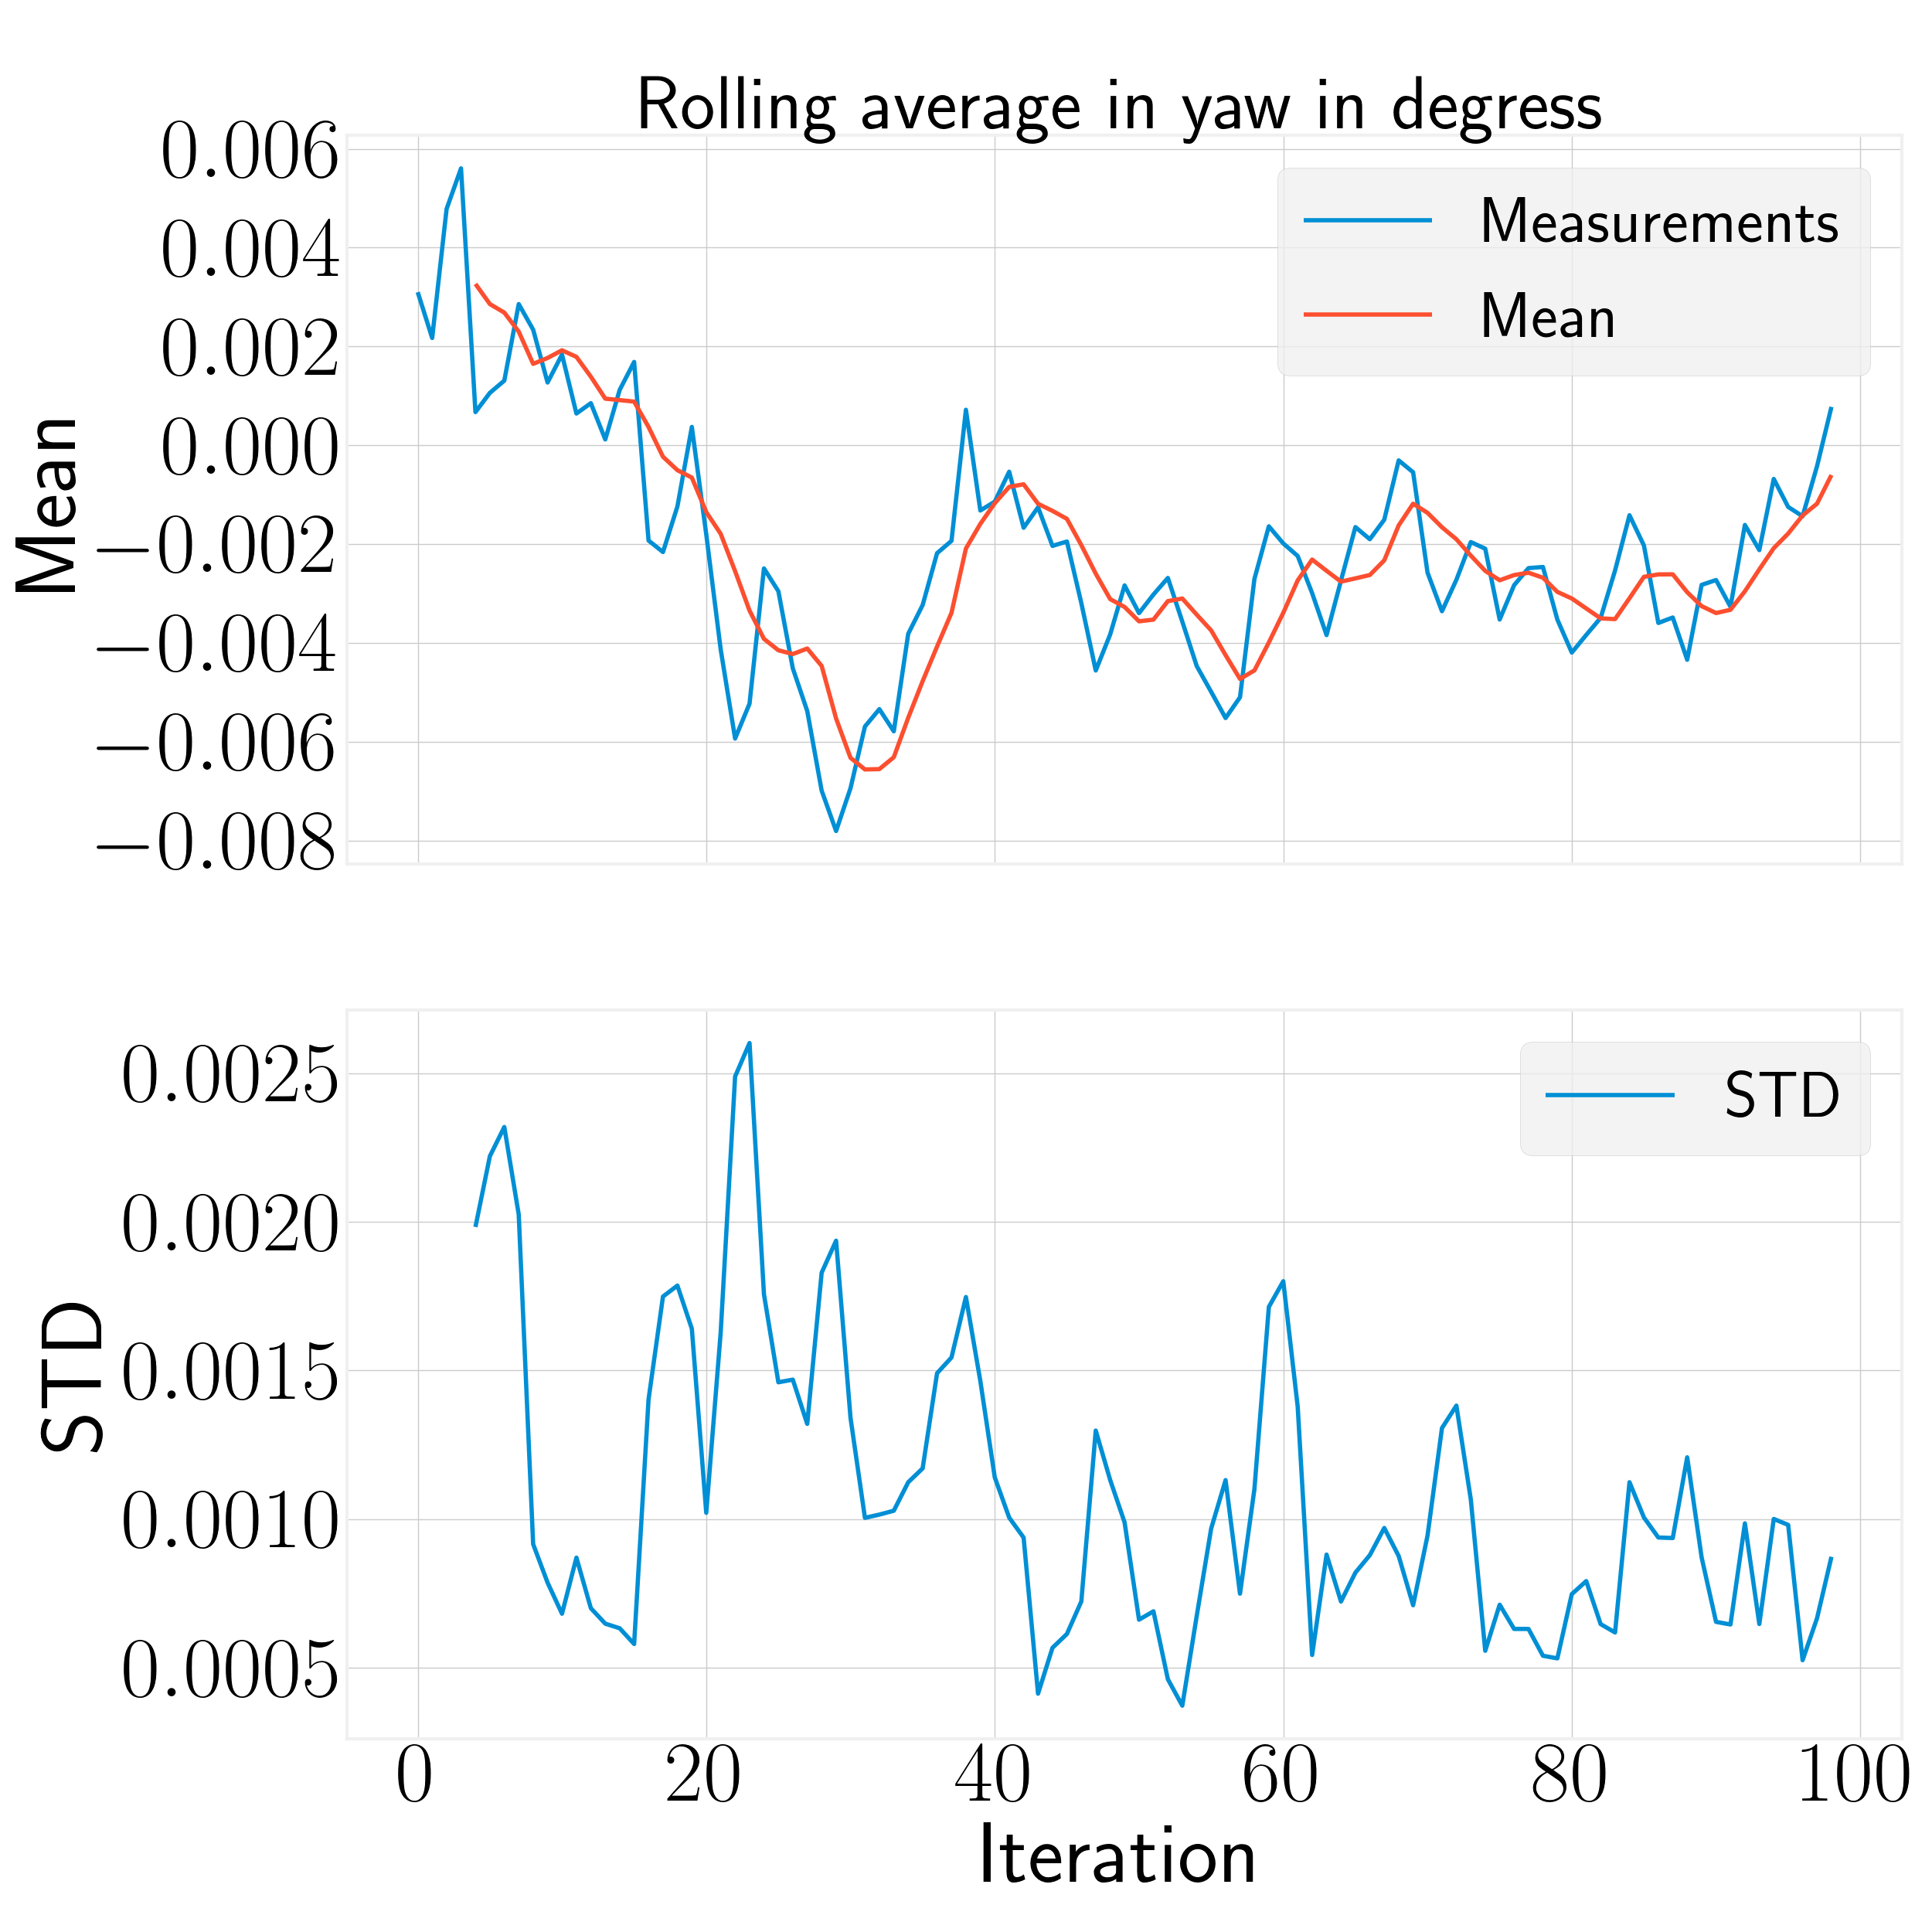
\includegraphics[width=\textwidth]{../Figures/analyse_rolling_average/test1/Calculated_rolling_average_in_yaw_with_mean_and_STD.png}
        \caption{}
        \label{fig:rolling_average_in_yaw_test1}
    \end{subfigure}
    \caption{Illustrations of the rolling average from the configuration in Figure \ref{fig:rolling_average_good_pos}. As it can be seen, the fluctuations in the angle estimates are steady with only negligible deviations}
    \label{fig:rolling_average_angle_test1}
\end{figure}

\begin{figure}[H]
    \centering
    \begin{subfigure}[t]{.30\textwidth}
        \centering
        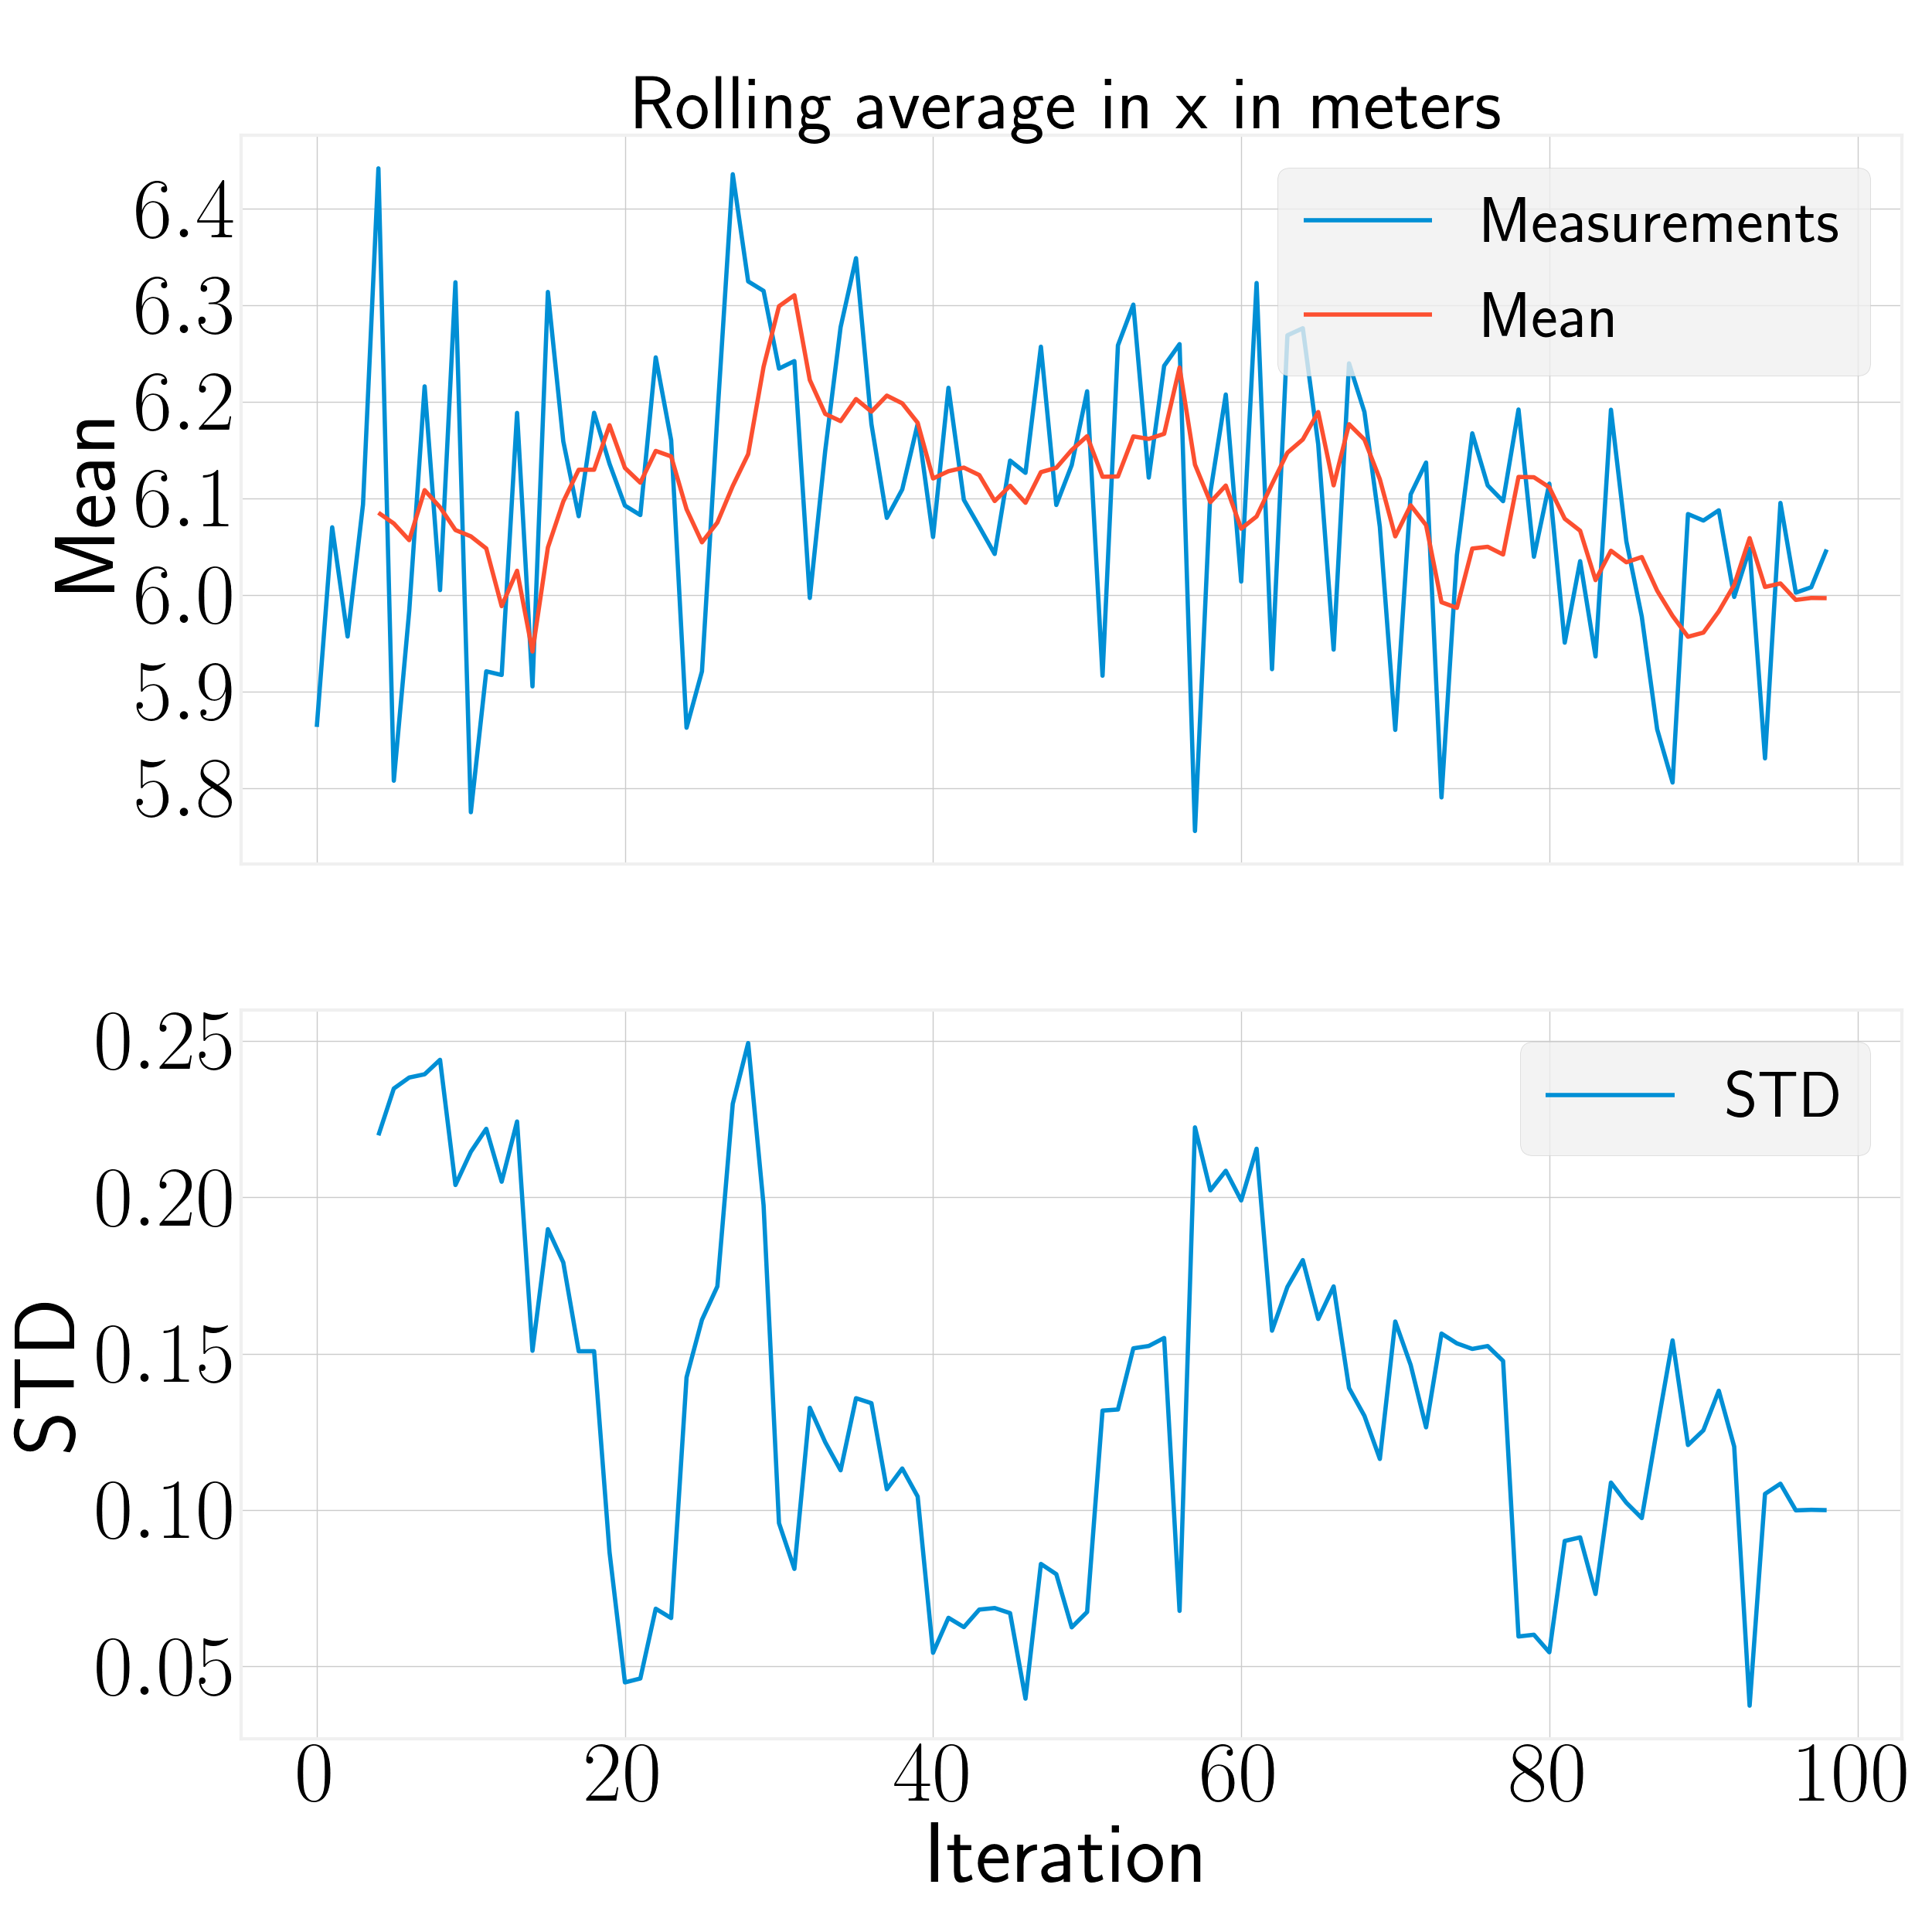
\includegraphics[width=\textwidth]{../Figures/analyse_rolling_average/test2/Calculated_rolling_average_in_x_with_mean_and_STD.png}
        \caption{}
        \label{fig:rolling_average_in_x_test2}
    \end{subfigure}
     \hspace{0.2em}
    \begin{subfigure}[t]{.30\textwidth}
        \centering
        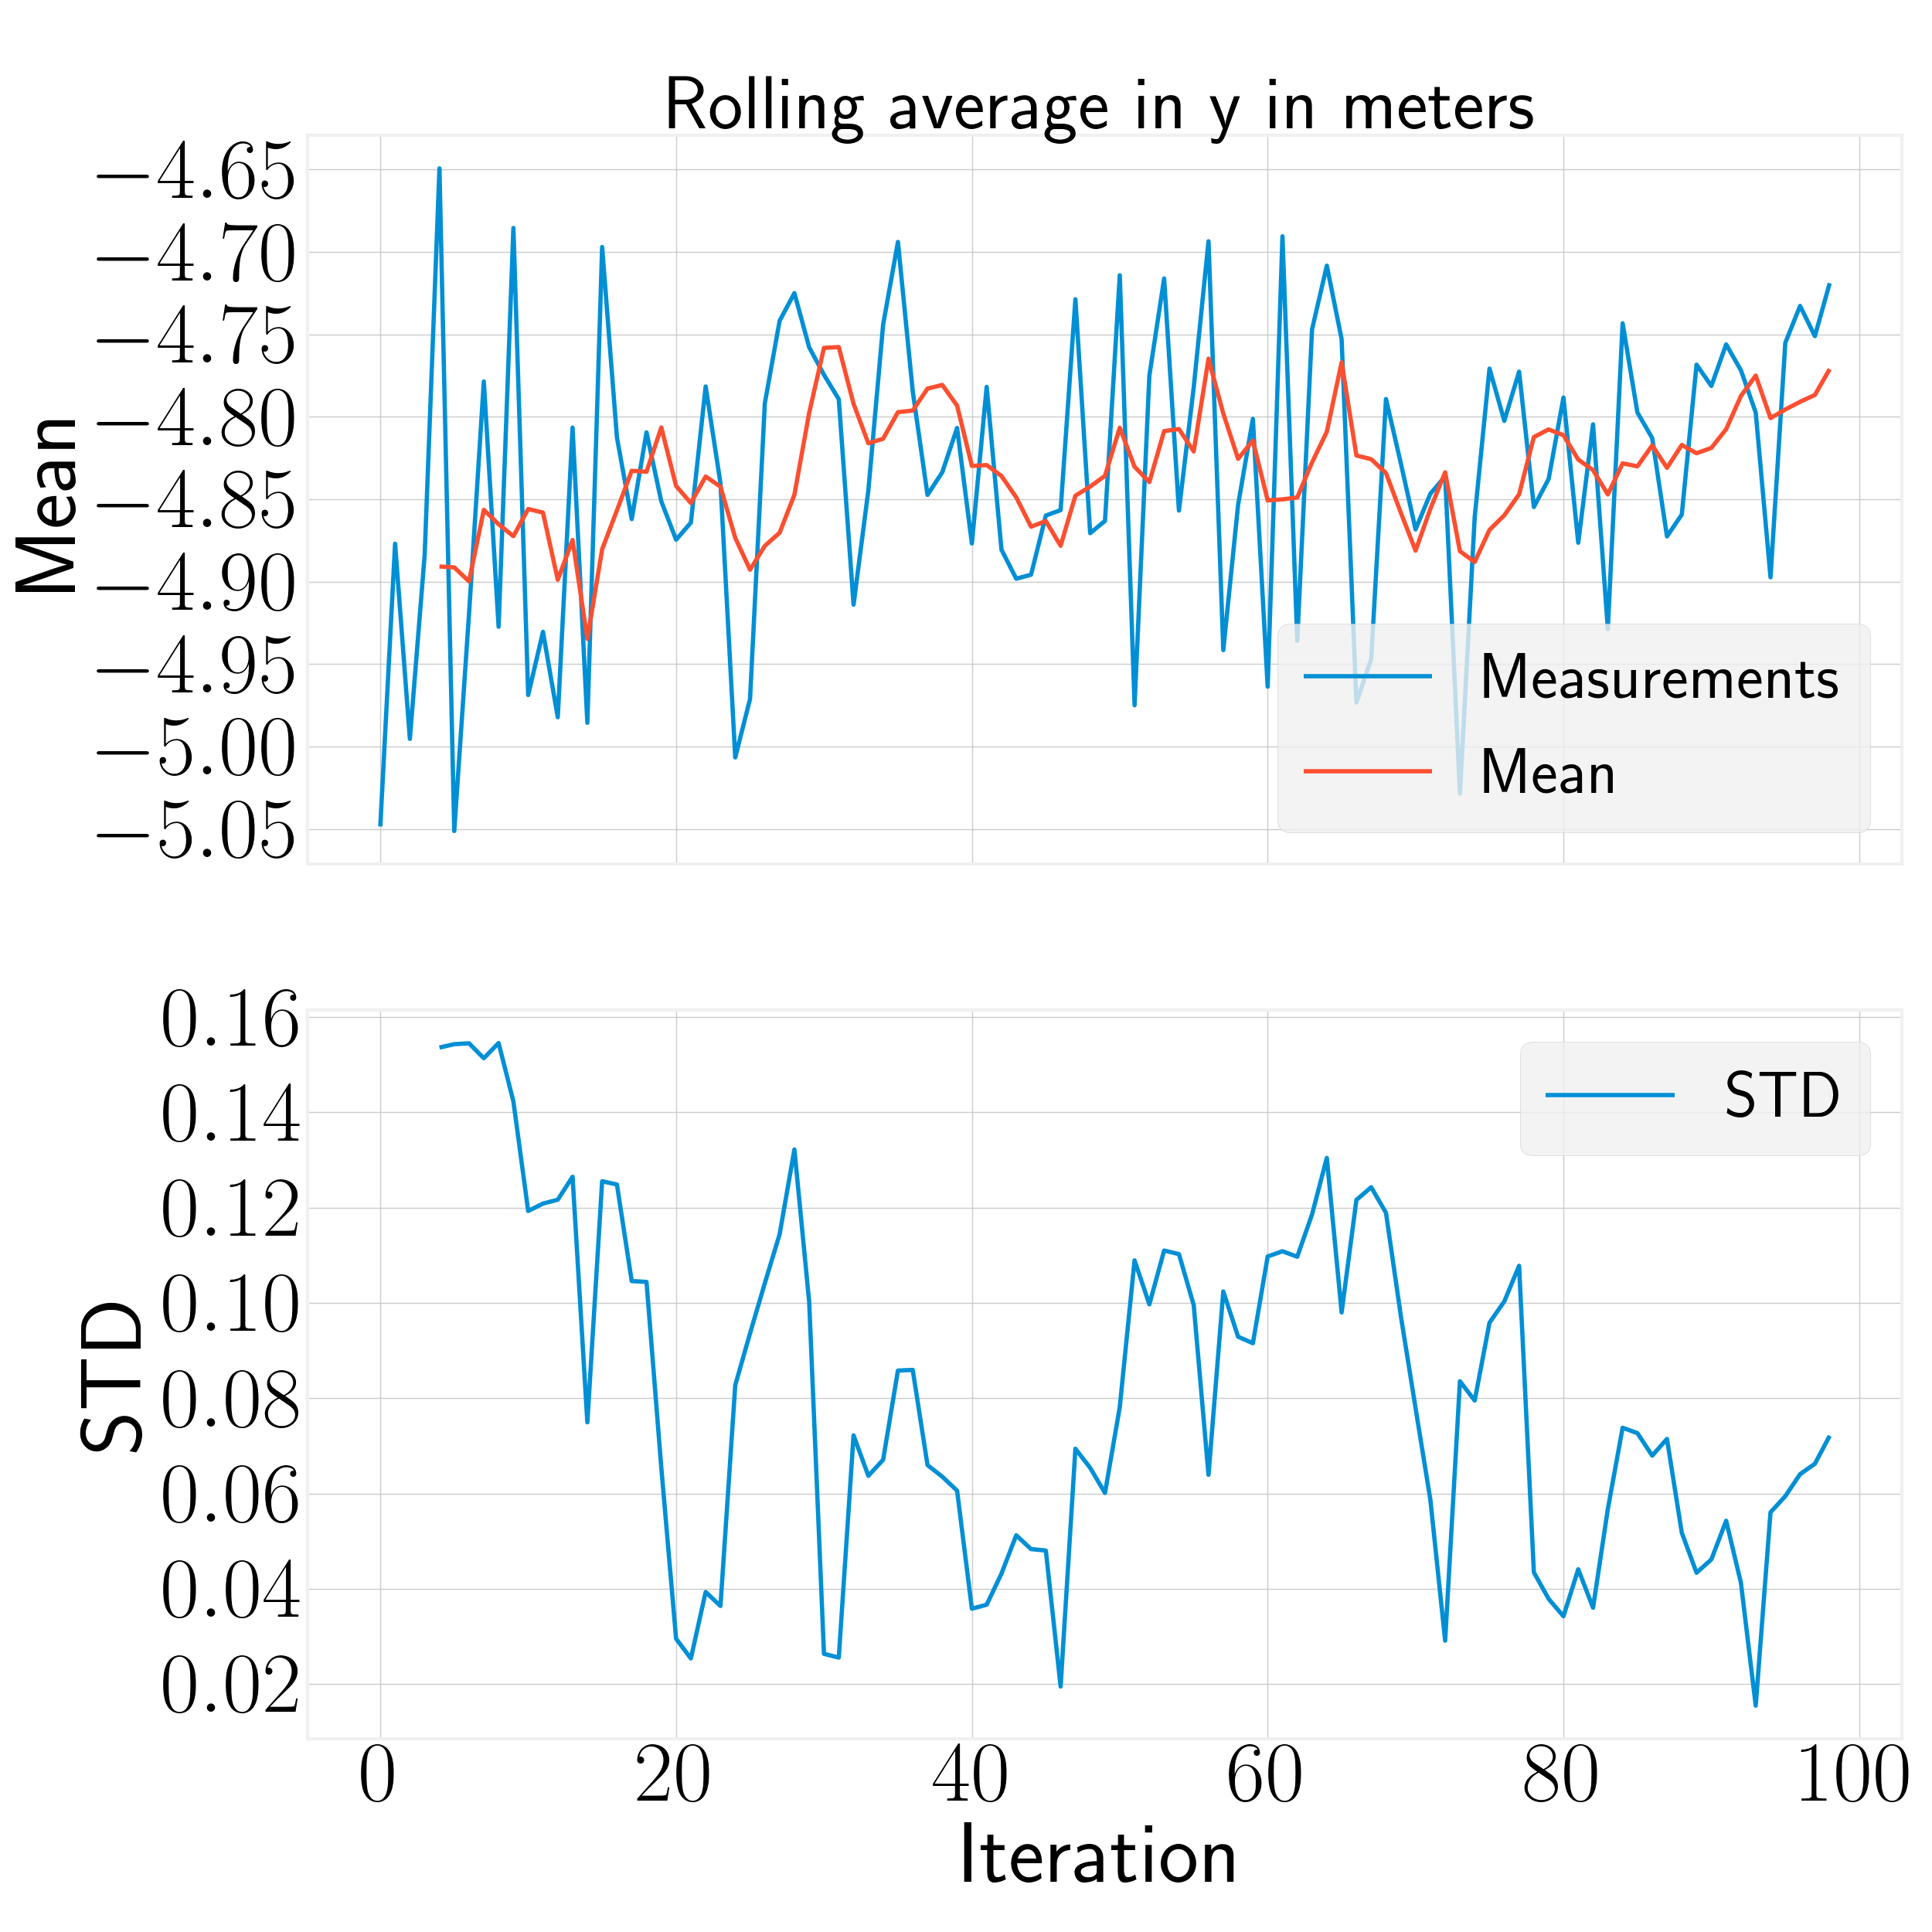
\includegraphics[width=\textwidth]{../Figures/analyse_rolling_average/test2/Calculated_rolling_average_in_y_with_mean_and_STD.png}
        \caption{}
        \label{fig:rolling_average_in_y_test2}
    \end{subfigure}
     \hspace{0.2em}
    \begin{subfigure}[t]{.30\textwidth}
        \centering
        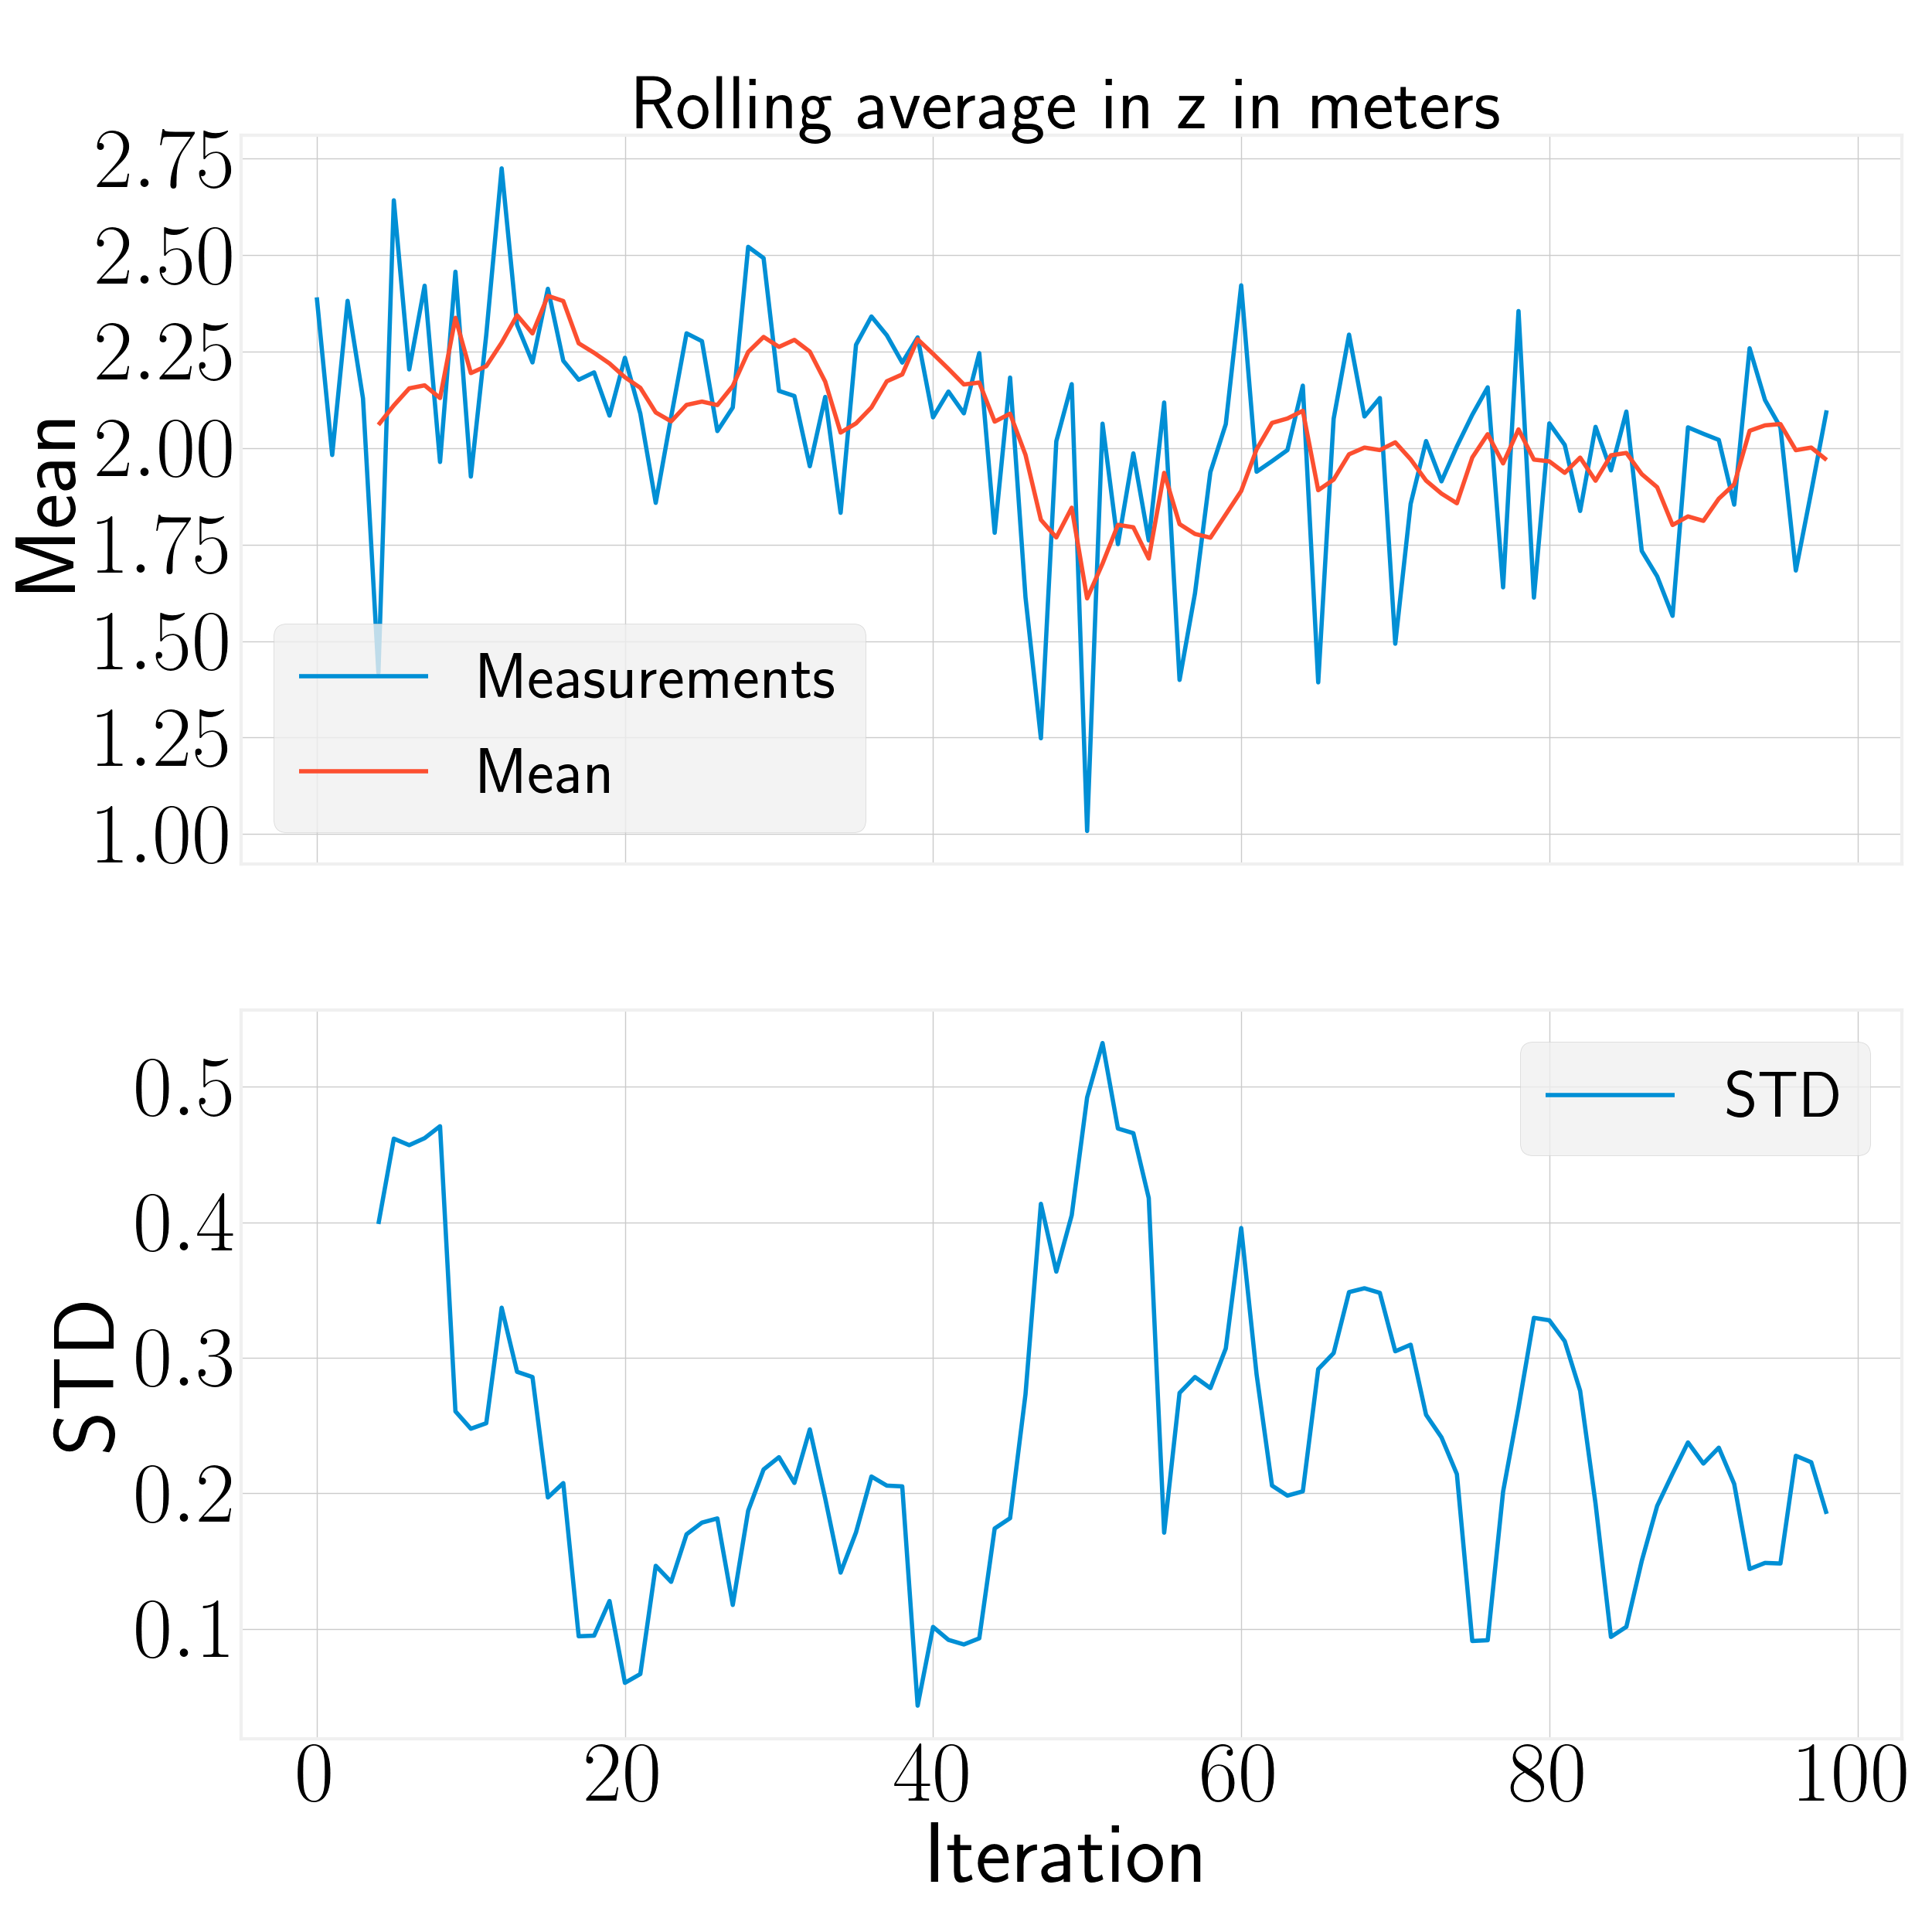
\includegraphics[width=\textwidth]{../Figures/analyse_rolling_average/test2/Calculated_rolling_average_in_z_with_mean_and_STD.png}
        \caption{}
        \label{fig:rolling_average_in_z_test2}
    \end{subfigure}
    \caption{Illustrations of the rolling average from the configuration in Figure \ref{fig:rolling_average_bad_pos}. As it can be seen, the fluctuations of the position estimates fluctuates a lot especially in the altitude}
    \label{fig:rolling_average_pos_test2}
\end{figure}

\begin{figure}[H]
    \centering
    \begin{subfigure}[t]{.30\textwidth}
        \centering
        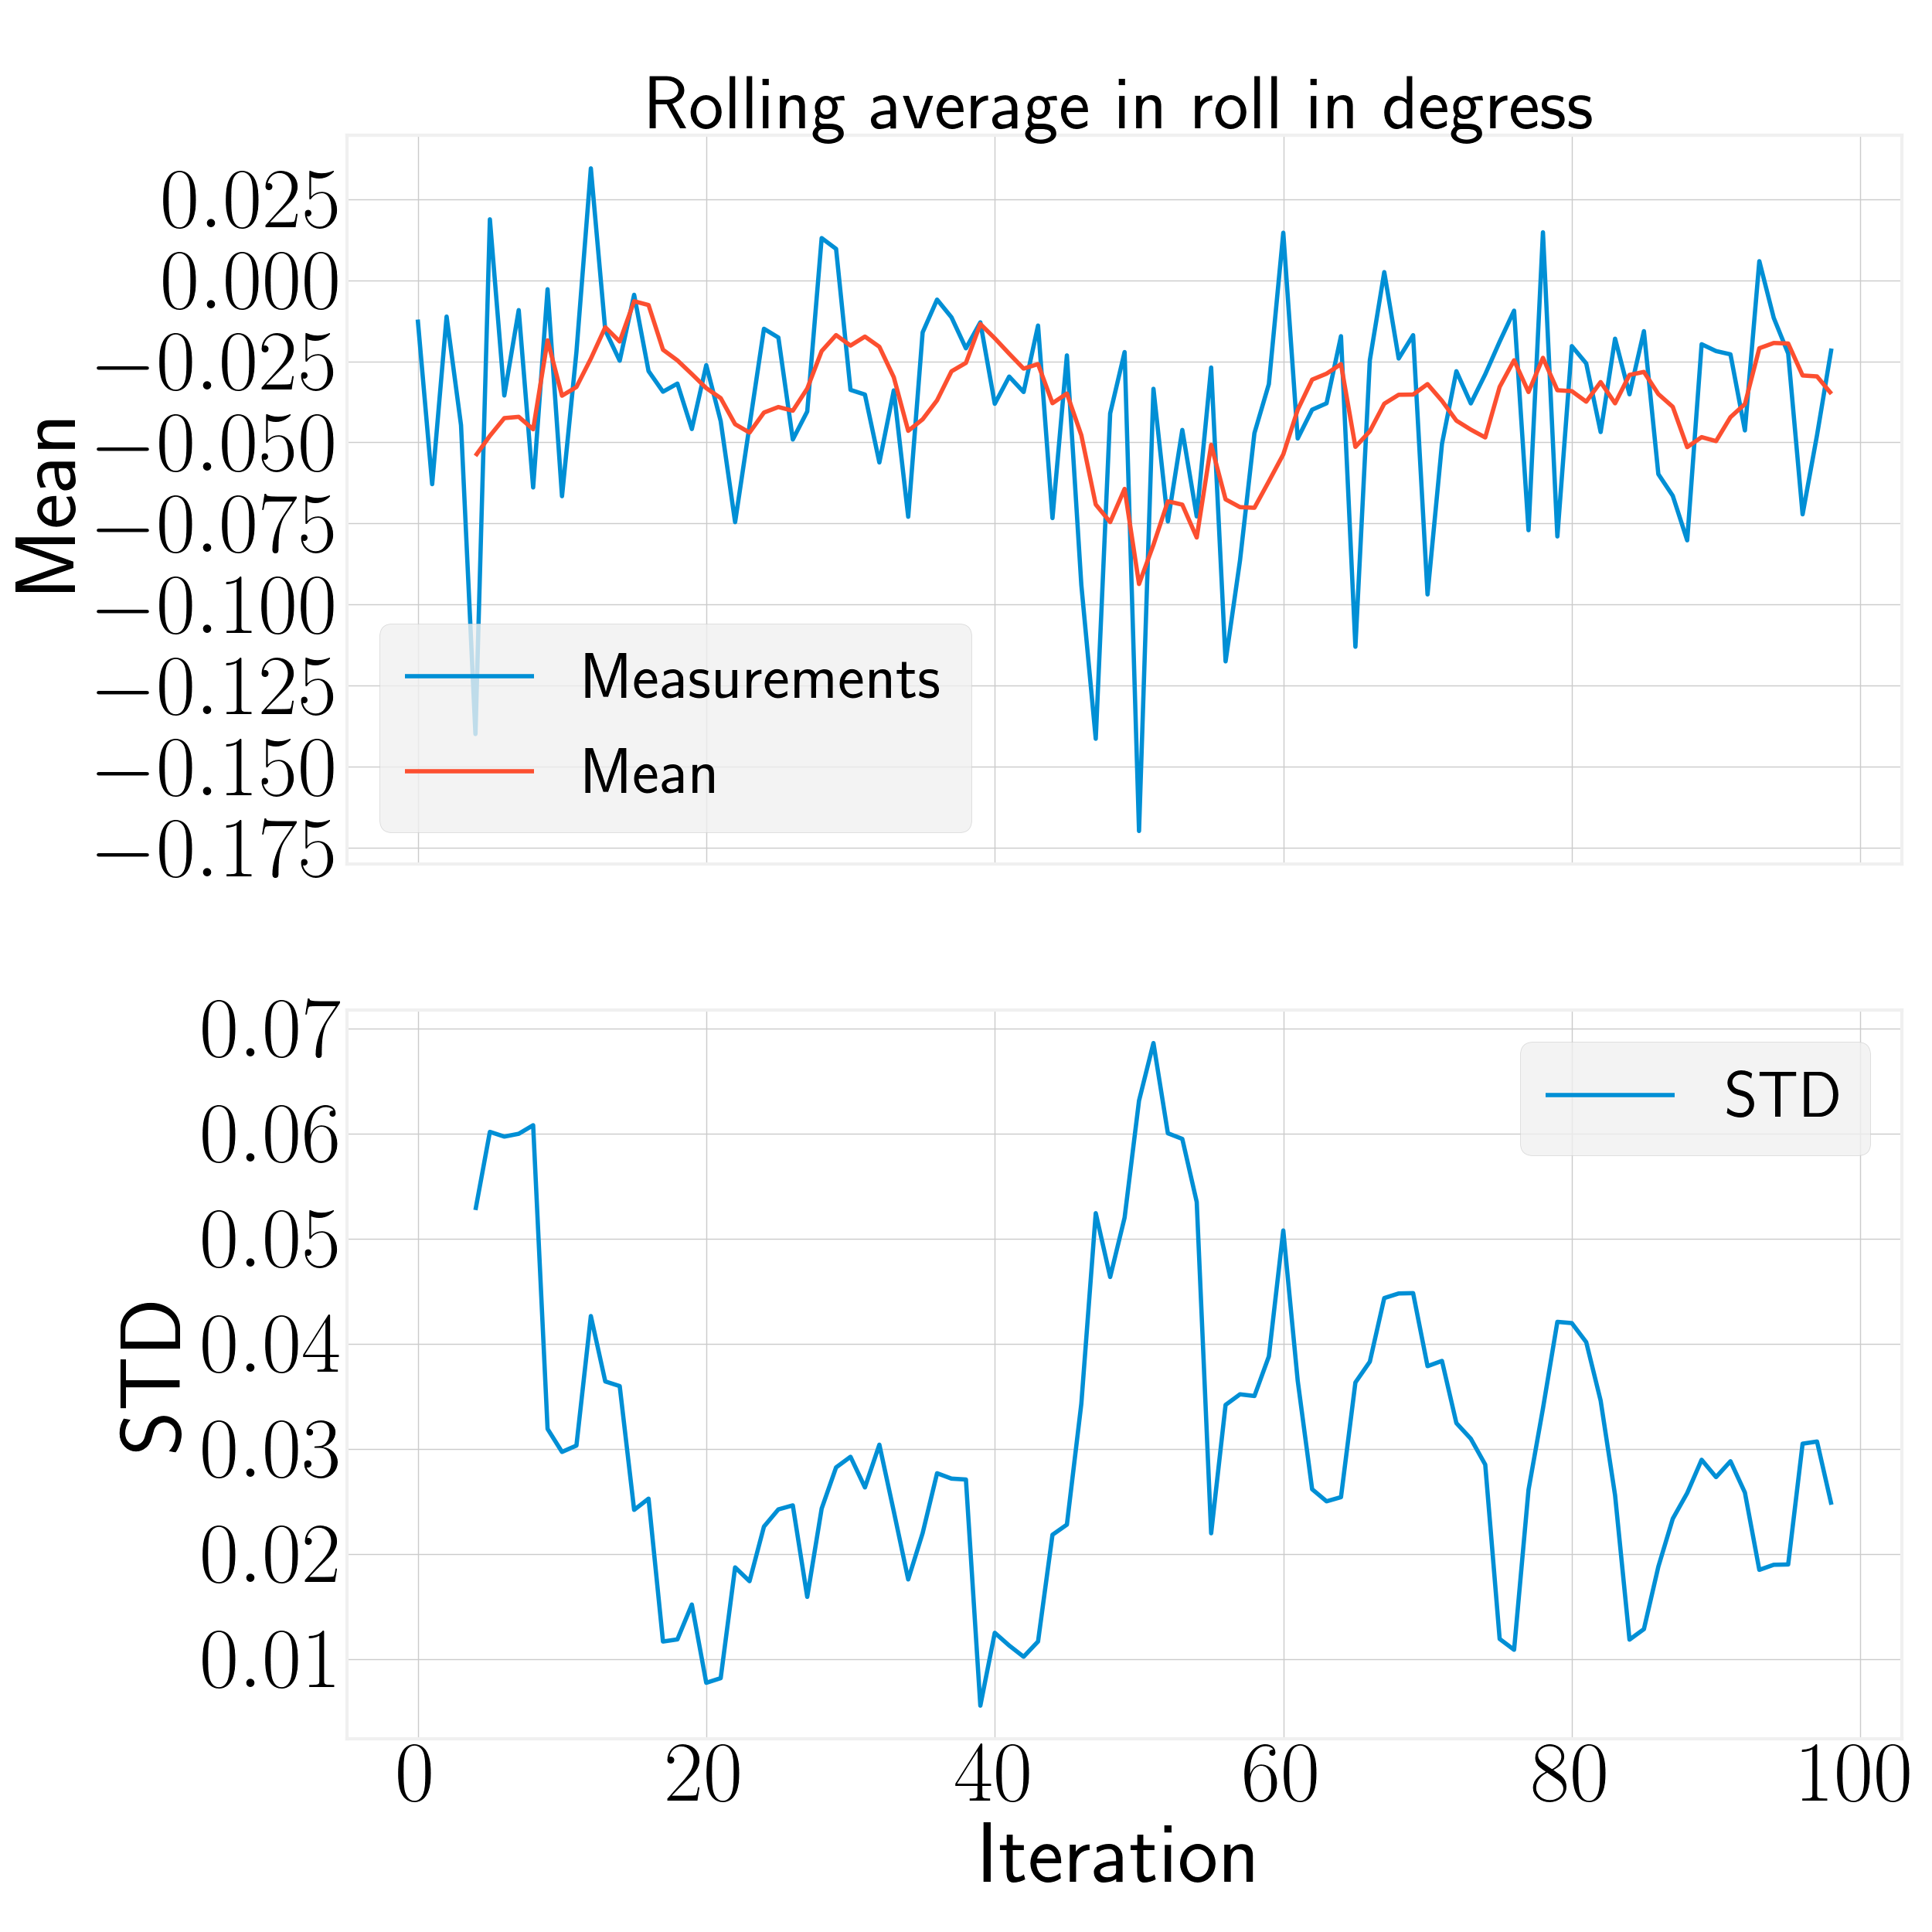
\includegraphics[width=\textwidth]{../Figures/analyse_rolling_average/test2/Calculated_rolling_average_in_roll_with_mean_and_STD.png}
        \caption{}
        \label{fig:rolling_average_in_roll_test2}
    \end{subfigure}
     \hspace{0.2em}
    \begin{subfigure}[t]{.30\textwidth}
        \centering
        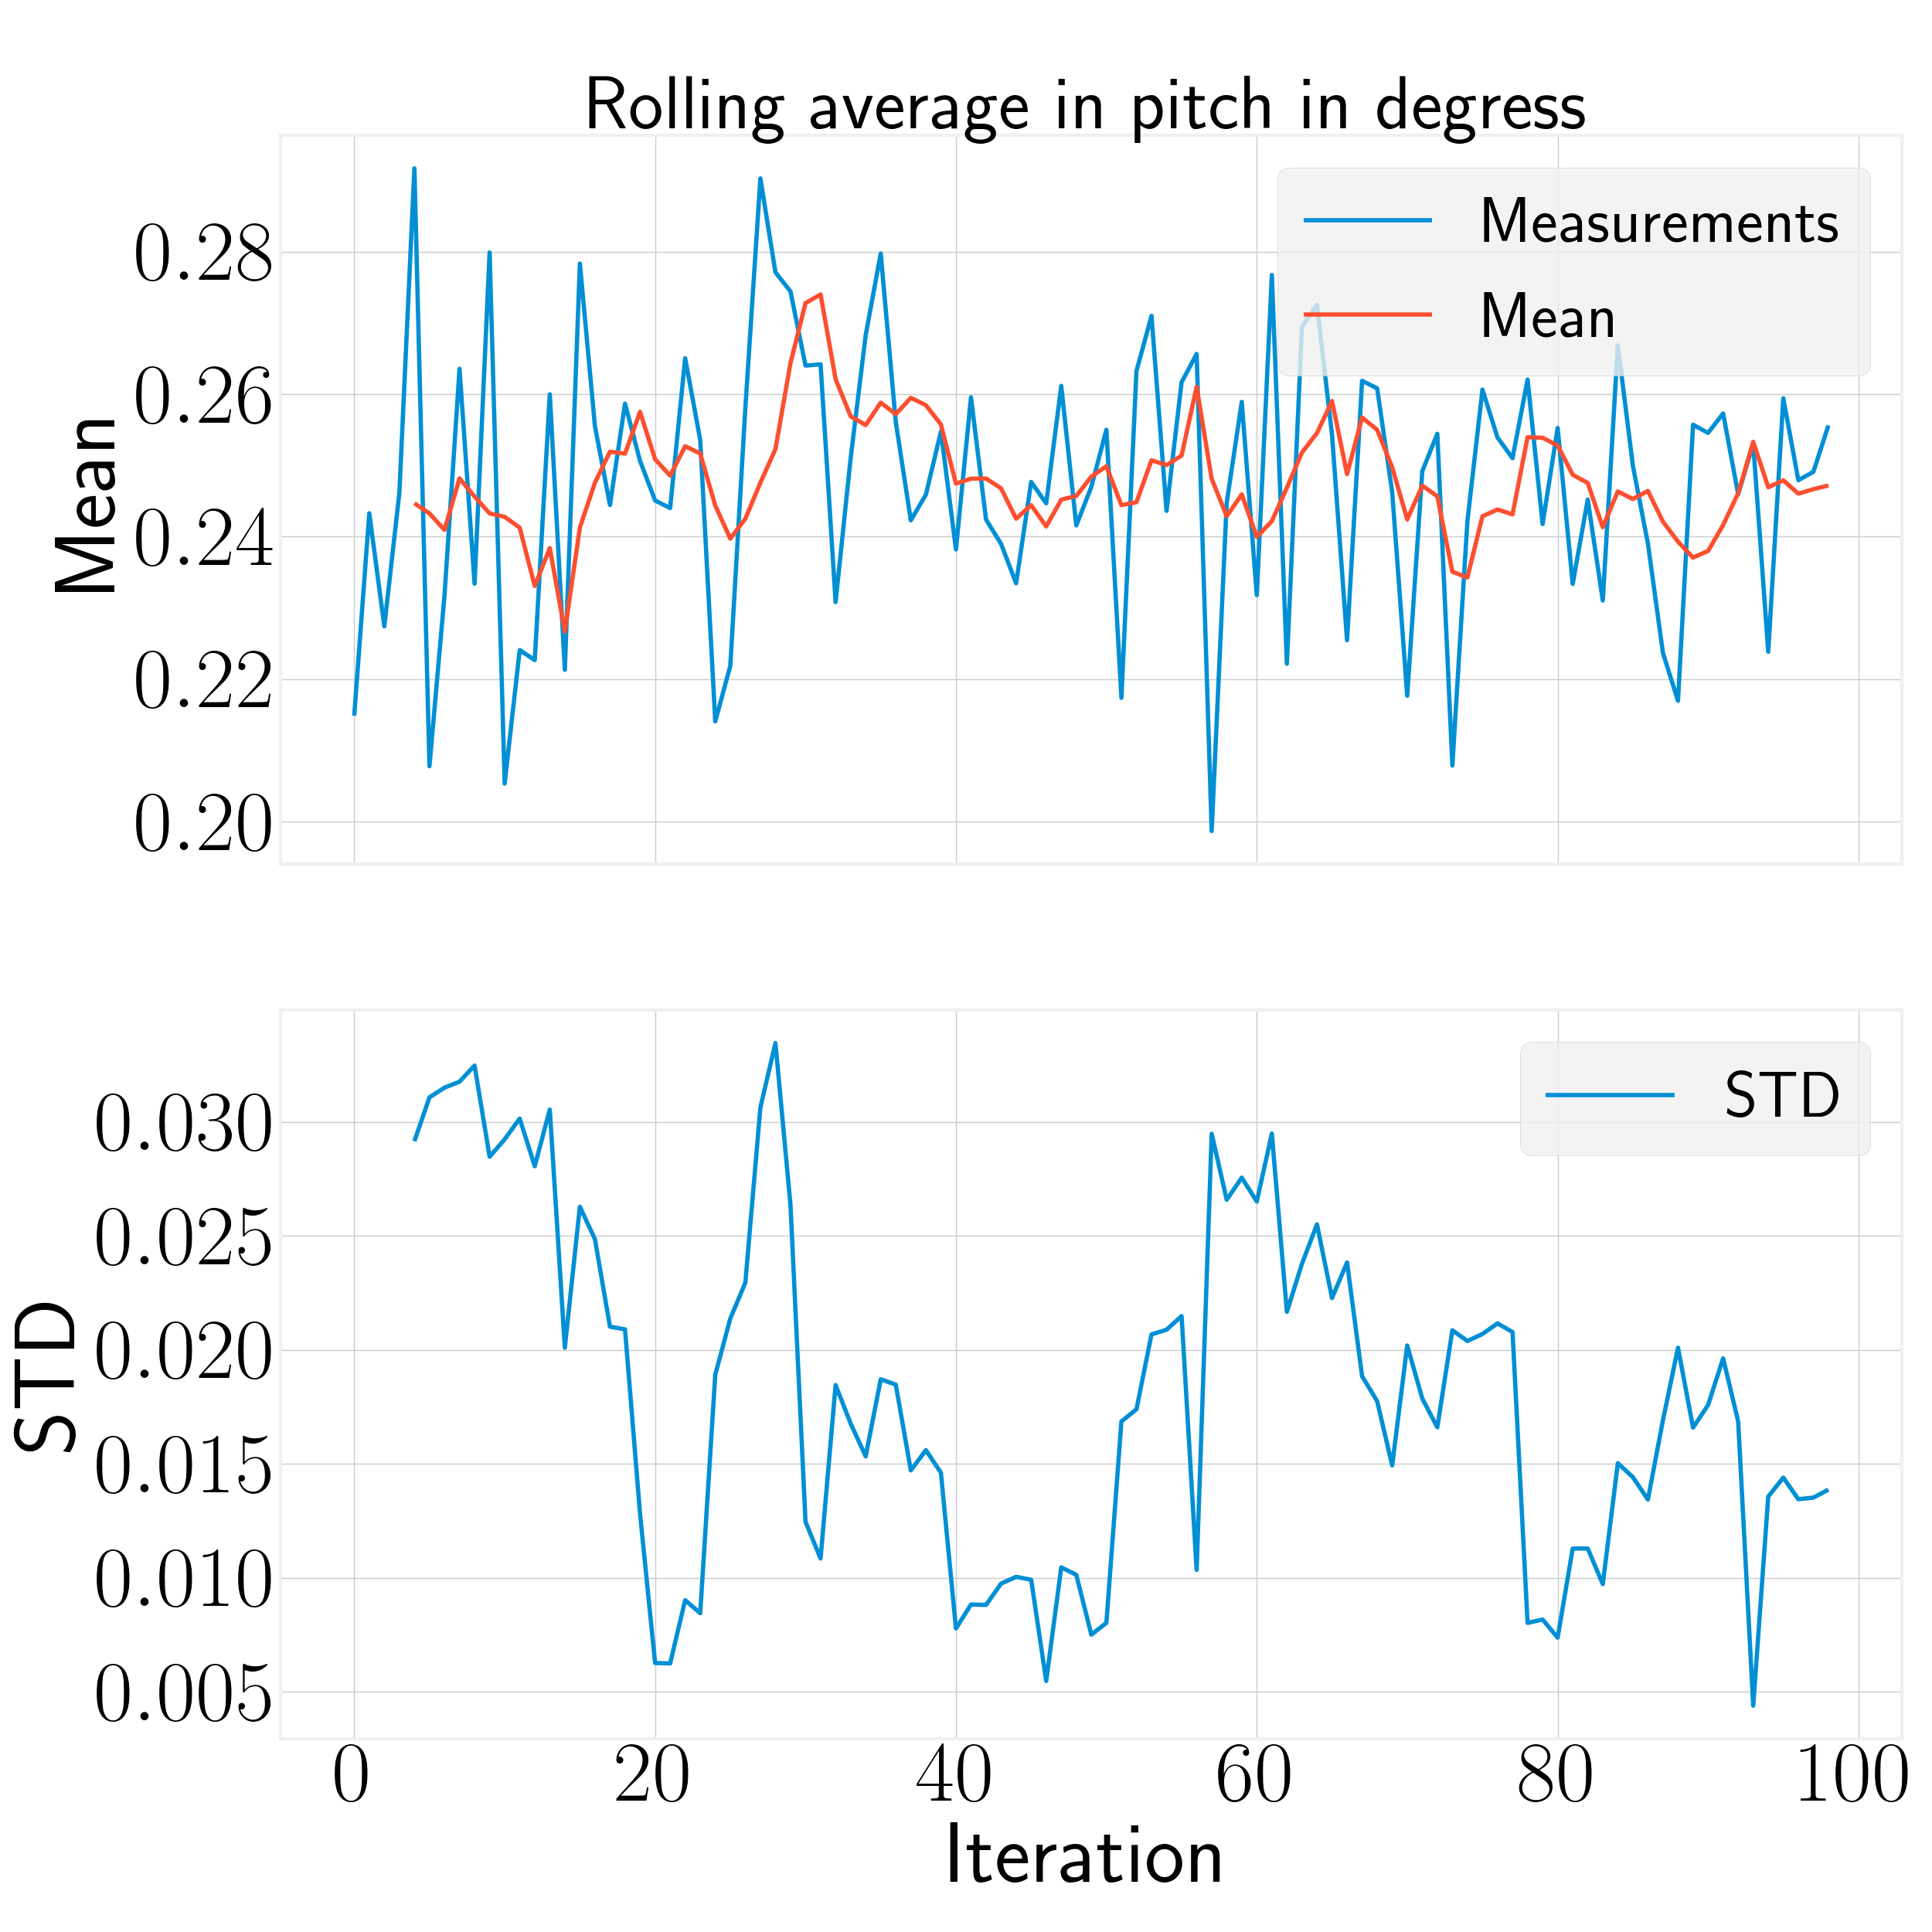
\includegraphics[width=\textwidth]{../Figures/analyse_rolling_average/test2/Calculated_rolling_average_in_pitch_with_mean_and_STD.png}
        \caption{}
        \label{fig:rolling_average_in_pitch_test2}
    \end{subfigure}
     \hspace{0.2em}
    \begin{subfigure}[t]{.30\textwidth}
        \centering
        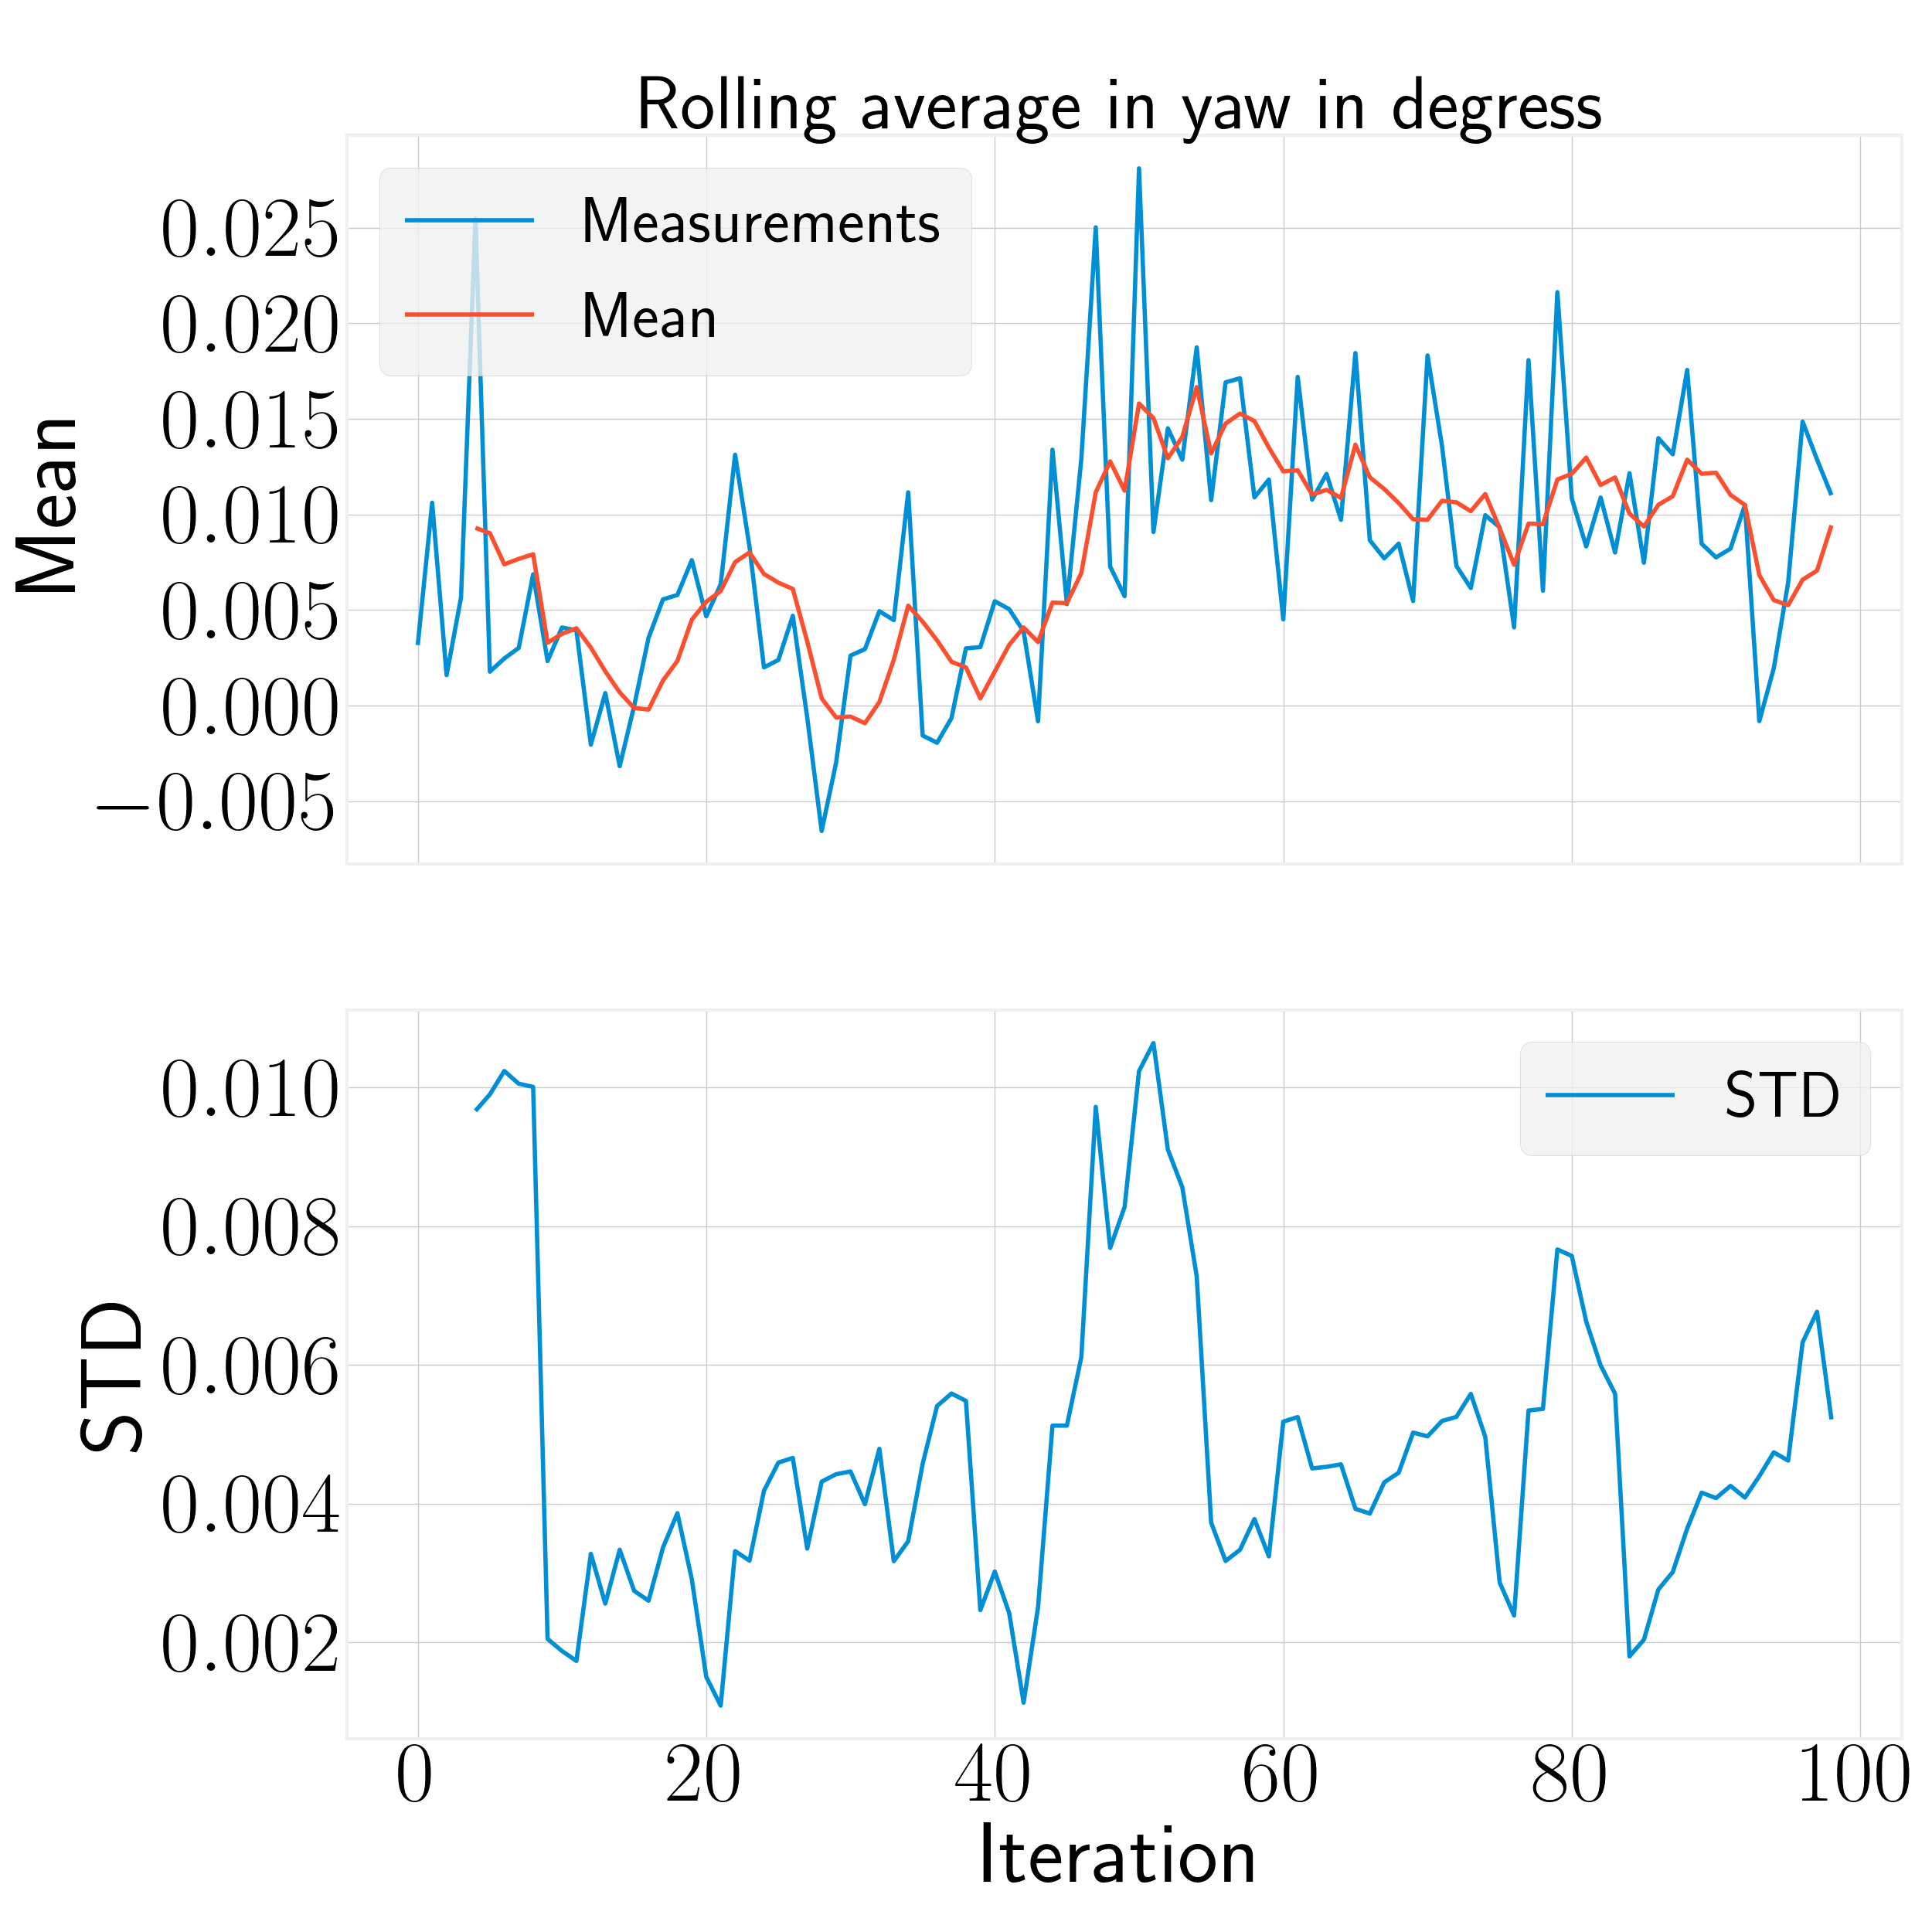
\includegraphics[width=\textwidth]{../Figures/analyse_rolling_average/test2/Calculated_rolling_average_in_yaw_with_mean_and_STD.png}
        \caption{}
        \label{fig:rolling_average_in_yaw_test2}
    \end{subfigure}
    \caption{Illustrations of the rolling average from the configuration in Figure \ref{fig:rolling_average_bad_pos}. As it can be seen, the fluctuations in the angle are steady even in this configuration}
    \label{fig:rolling_average_angle_test2}
\end{figure}

As it can be seen in Figures \ref{fig:rolling_average_pos_test1} and \ref{fig:rolling_average_angle_test1}, the fluctuations in the estimates are only of minor concern when the drone is of a maximum distance of 5 meters from the GPS2Vision board. However, when the drone changes to a position outside of the \textit{safe area}, the estimations in position fluctuates a lot as seen in Figure \ref{fig:rolling_average_pos_test2}. This could be fatal to make a transition in this scenario and lead to an unstable system. The angle estimates are affected less as seen in Figure \ref{fig:rolling_average_angle_test2}.

The outcome of the rolling average will be used alongside the maximum distance to the GPS2Vision board for stability analysis before going from GPS to vision navigation in Section \ref{sec:gps2vision_transition}.  

\subsubsection{Hold pose using ArUco pose estimation}
\label{sec:hold_pose_using_aruco_pose_estimation}

\begin{figure}[H]
    \centering
    \begin{subfigure}[t]{.30\textwidth}
        \centering
        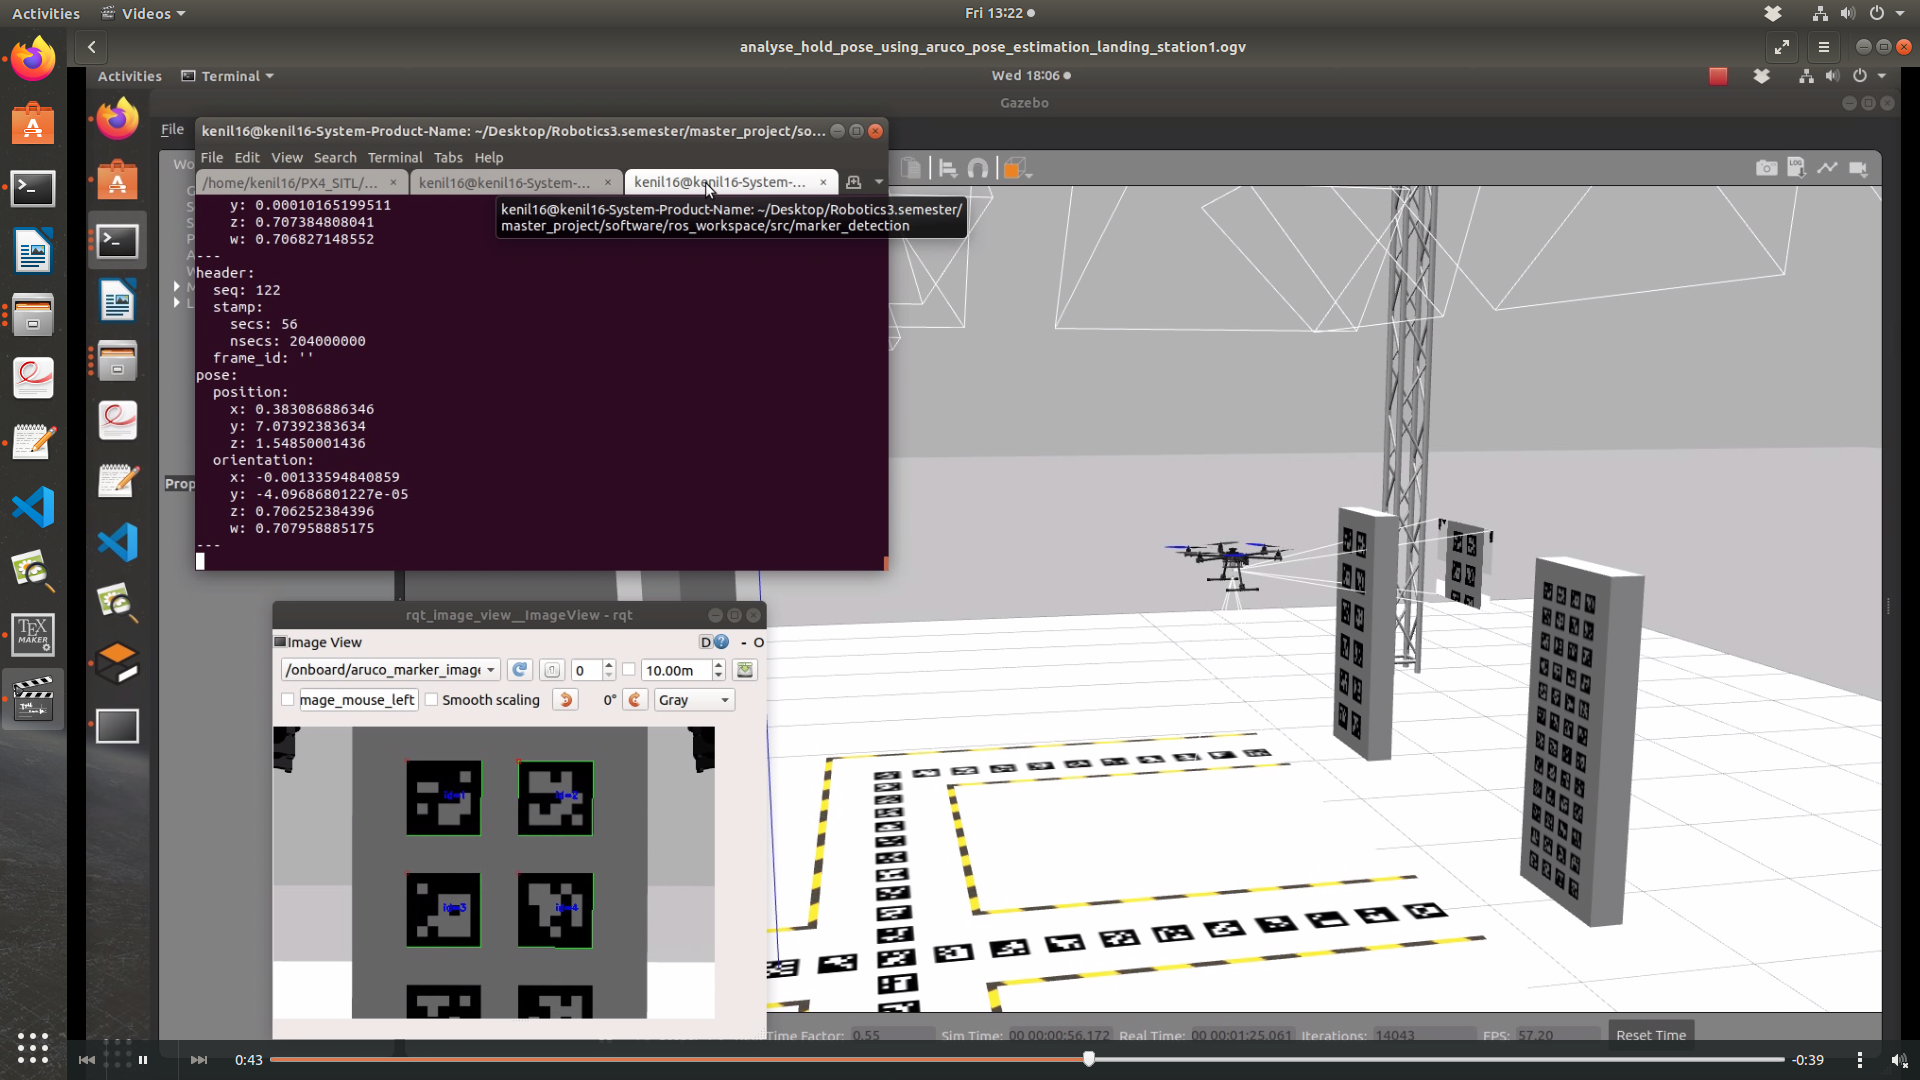
\includegraphics[width=\textwidth]{../Figures/hold_pose_using_aruco_pose_estimation/aruco_board_three.png}
        \caption{}
        \label{fig:hold_pose_aruco_board_three}
    \end{subfigure}
     \hspace{0.2em}
    \begin{subfigure}[t]{.30\textwidth}
        \centering
        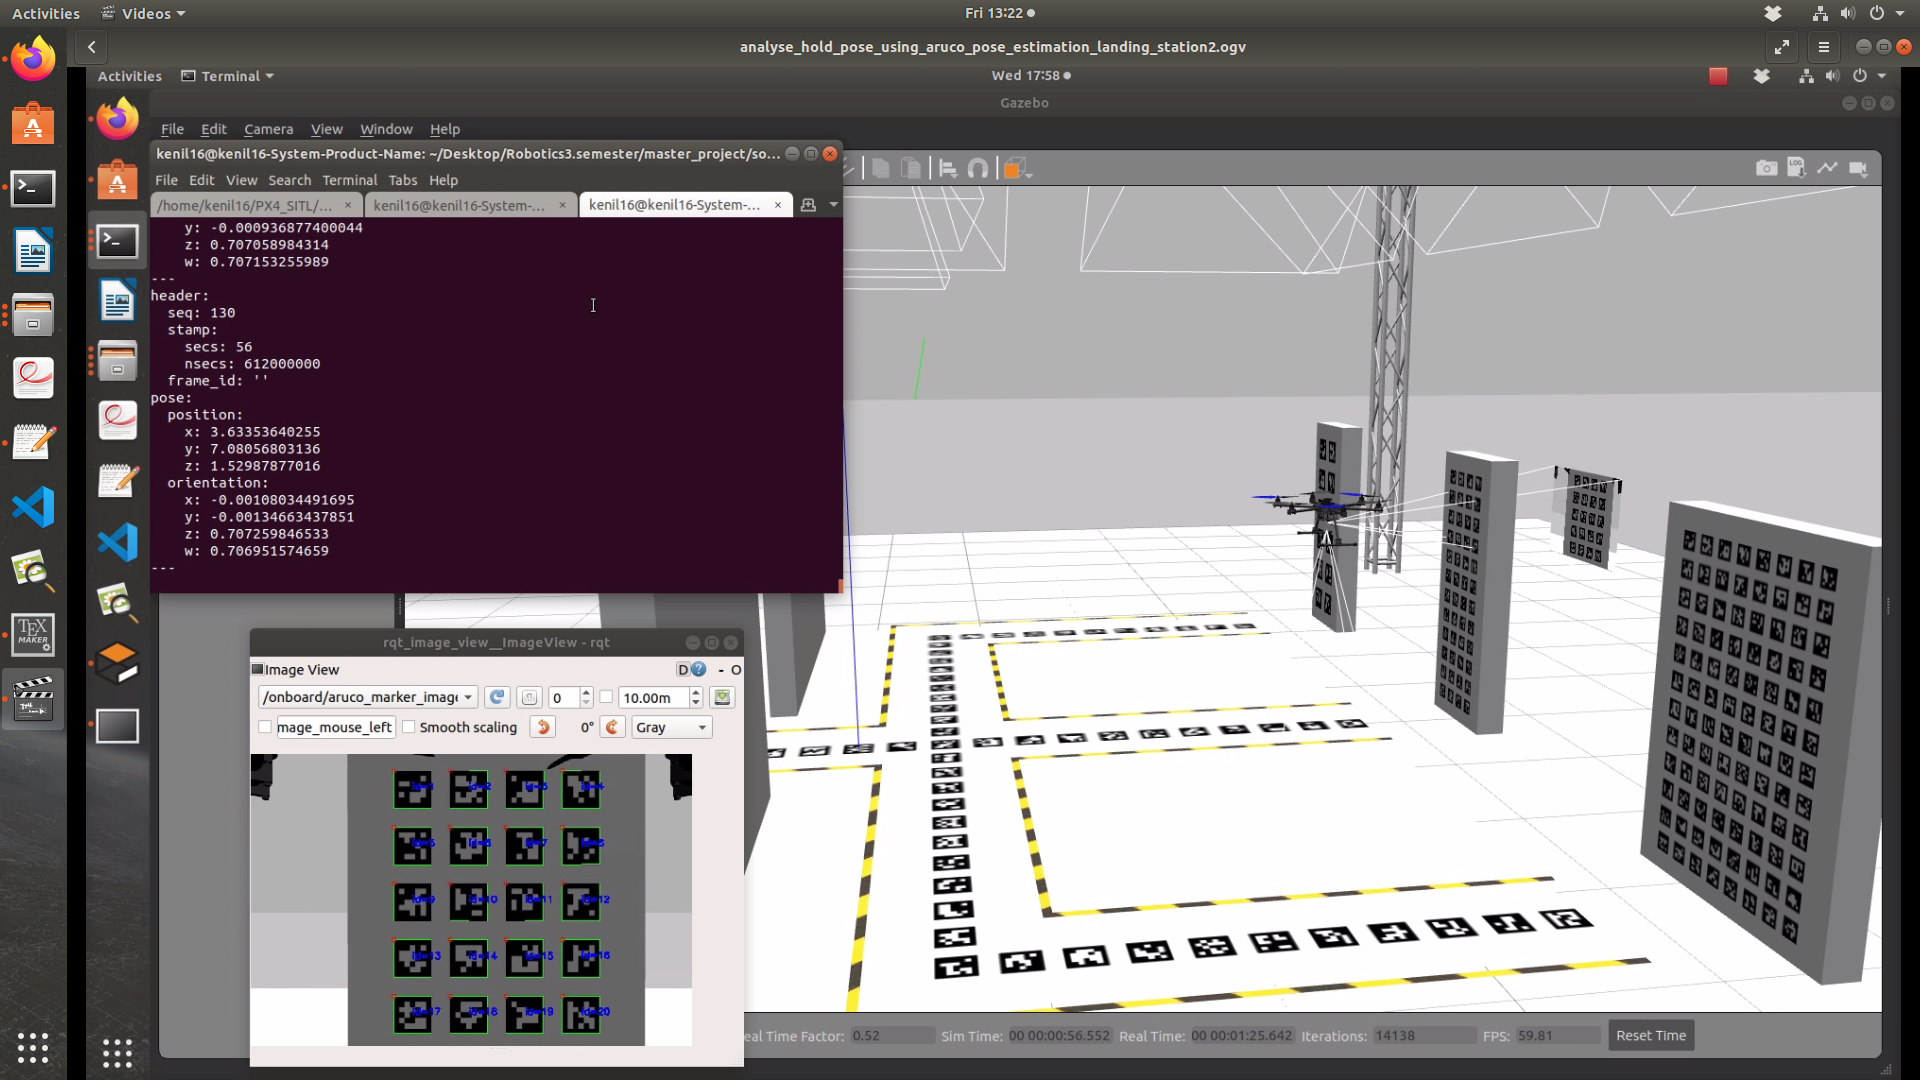
\includegraphics[width=\textwidth]{../Figures/hold_pose_using_aruco_pose_estimation/aruco_board_four.png}
        \caption{}
        \label{fig:hold_pose_aruco_board_four}
    \end{subfigure}
     \hspace{0.2em}
    \begin{subfigure}[t]{.30\textwidth}
        \centering
        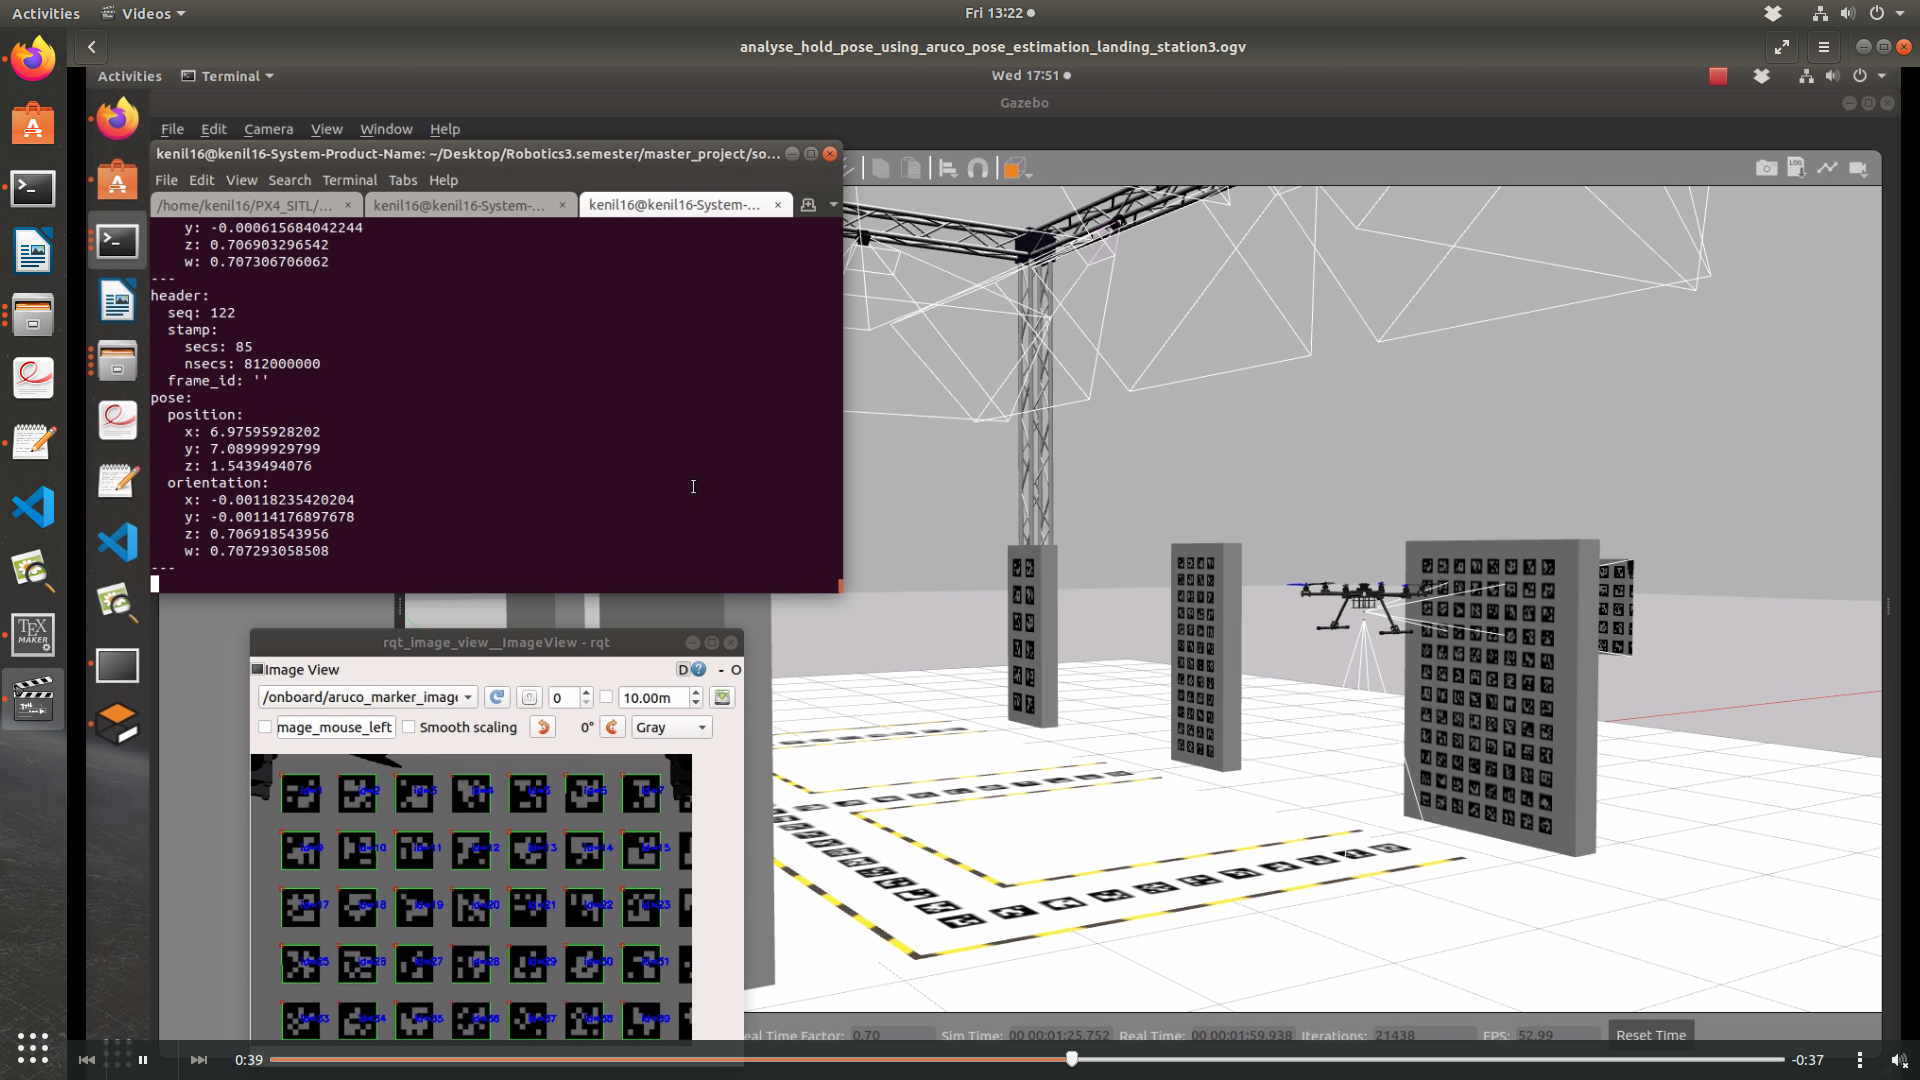
\includegraphics[width=\textwidth]{../Figures/hold_pose_using_aruco_pose_estimation/aruco_board_five.png}
        \caption{}
        \label{fig:hold_pose_aruco_board_five}
    \end{subfigure}
        \begin{subfigure}[t]{.30\textwidth}
        \centering
        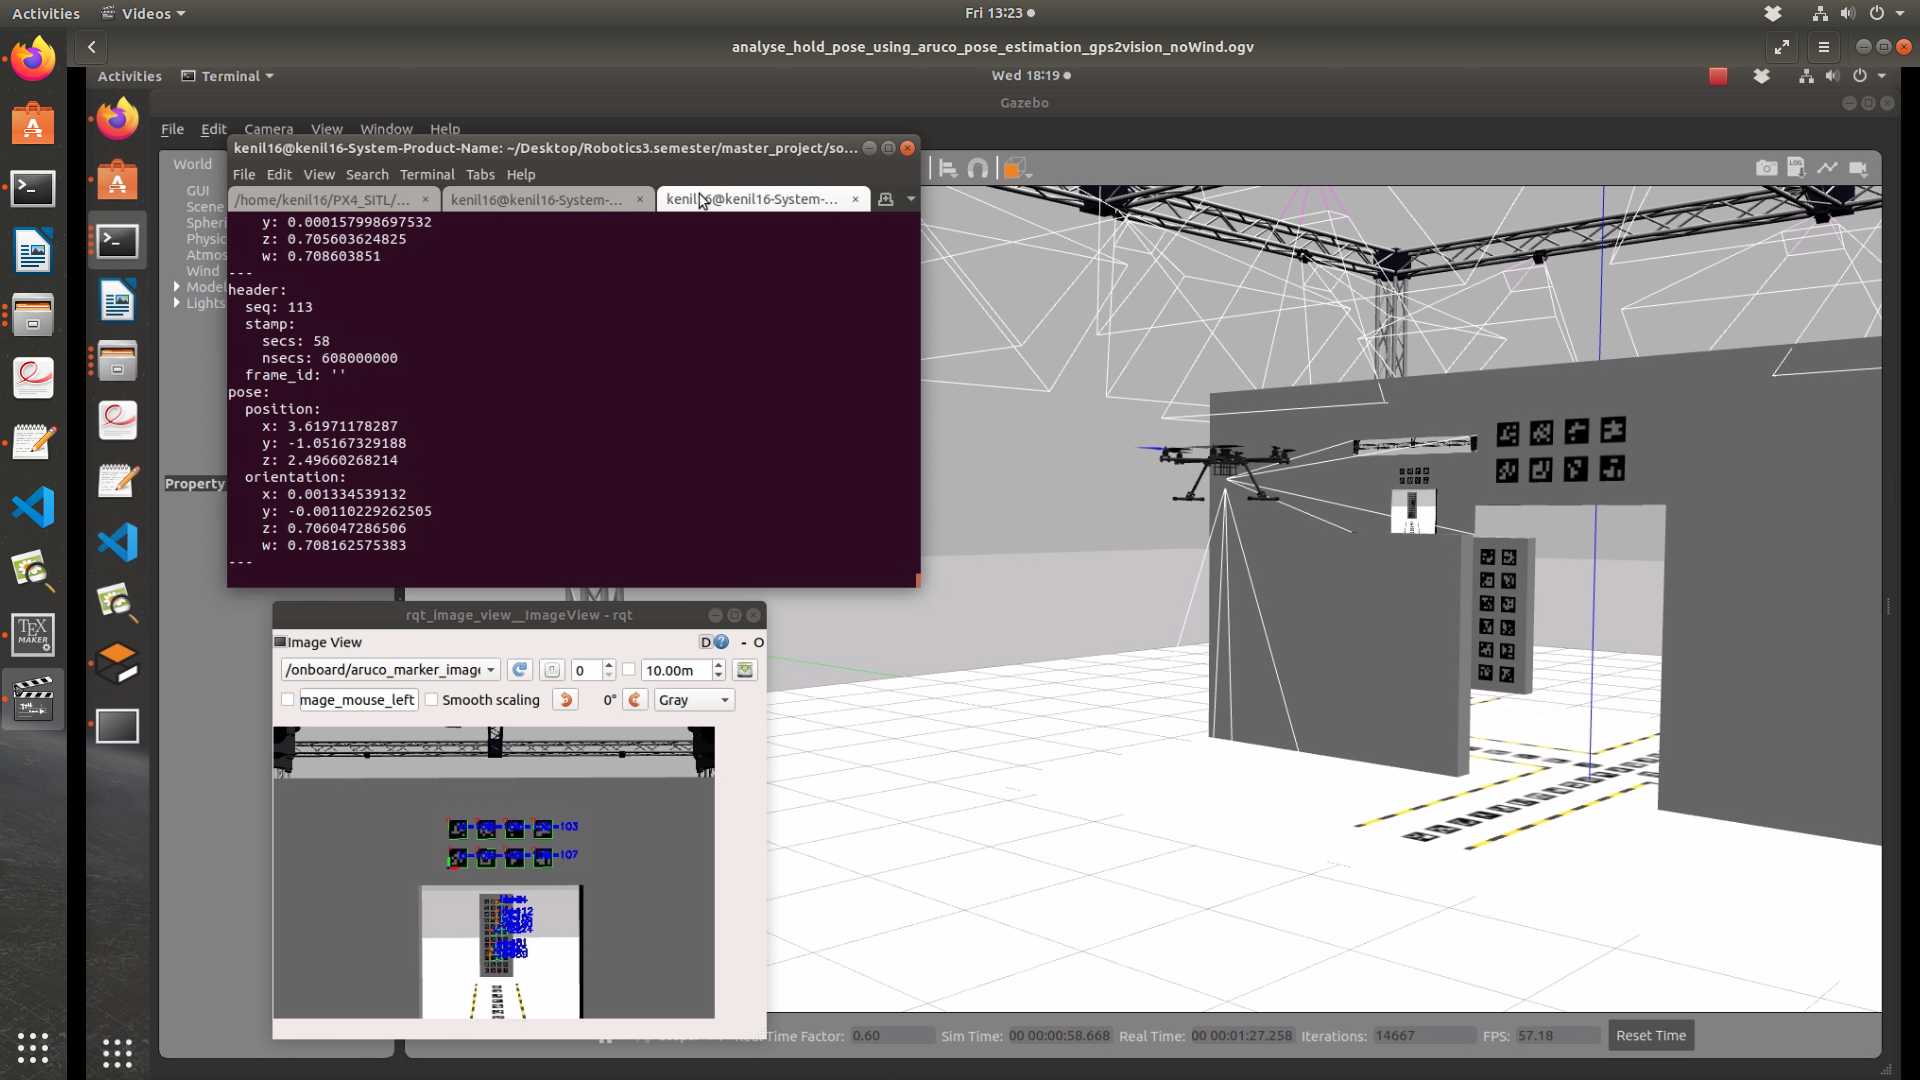
\includegraphics[width=\textwidth]{../Figures/hold_pose_using_aruco_pose_estimation/aruco_board_one_noWind.png}
        \caption{}
        \label{fig:hold_pose_aruco_board_one_noWind}
    \end{subfigure}
        \begin{subfigure}[t]{.30\textwidth}
        \centering
        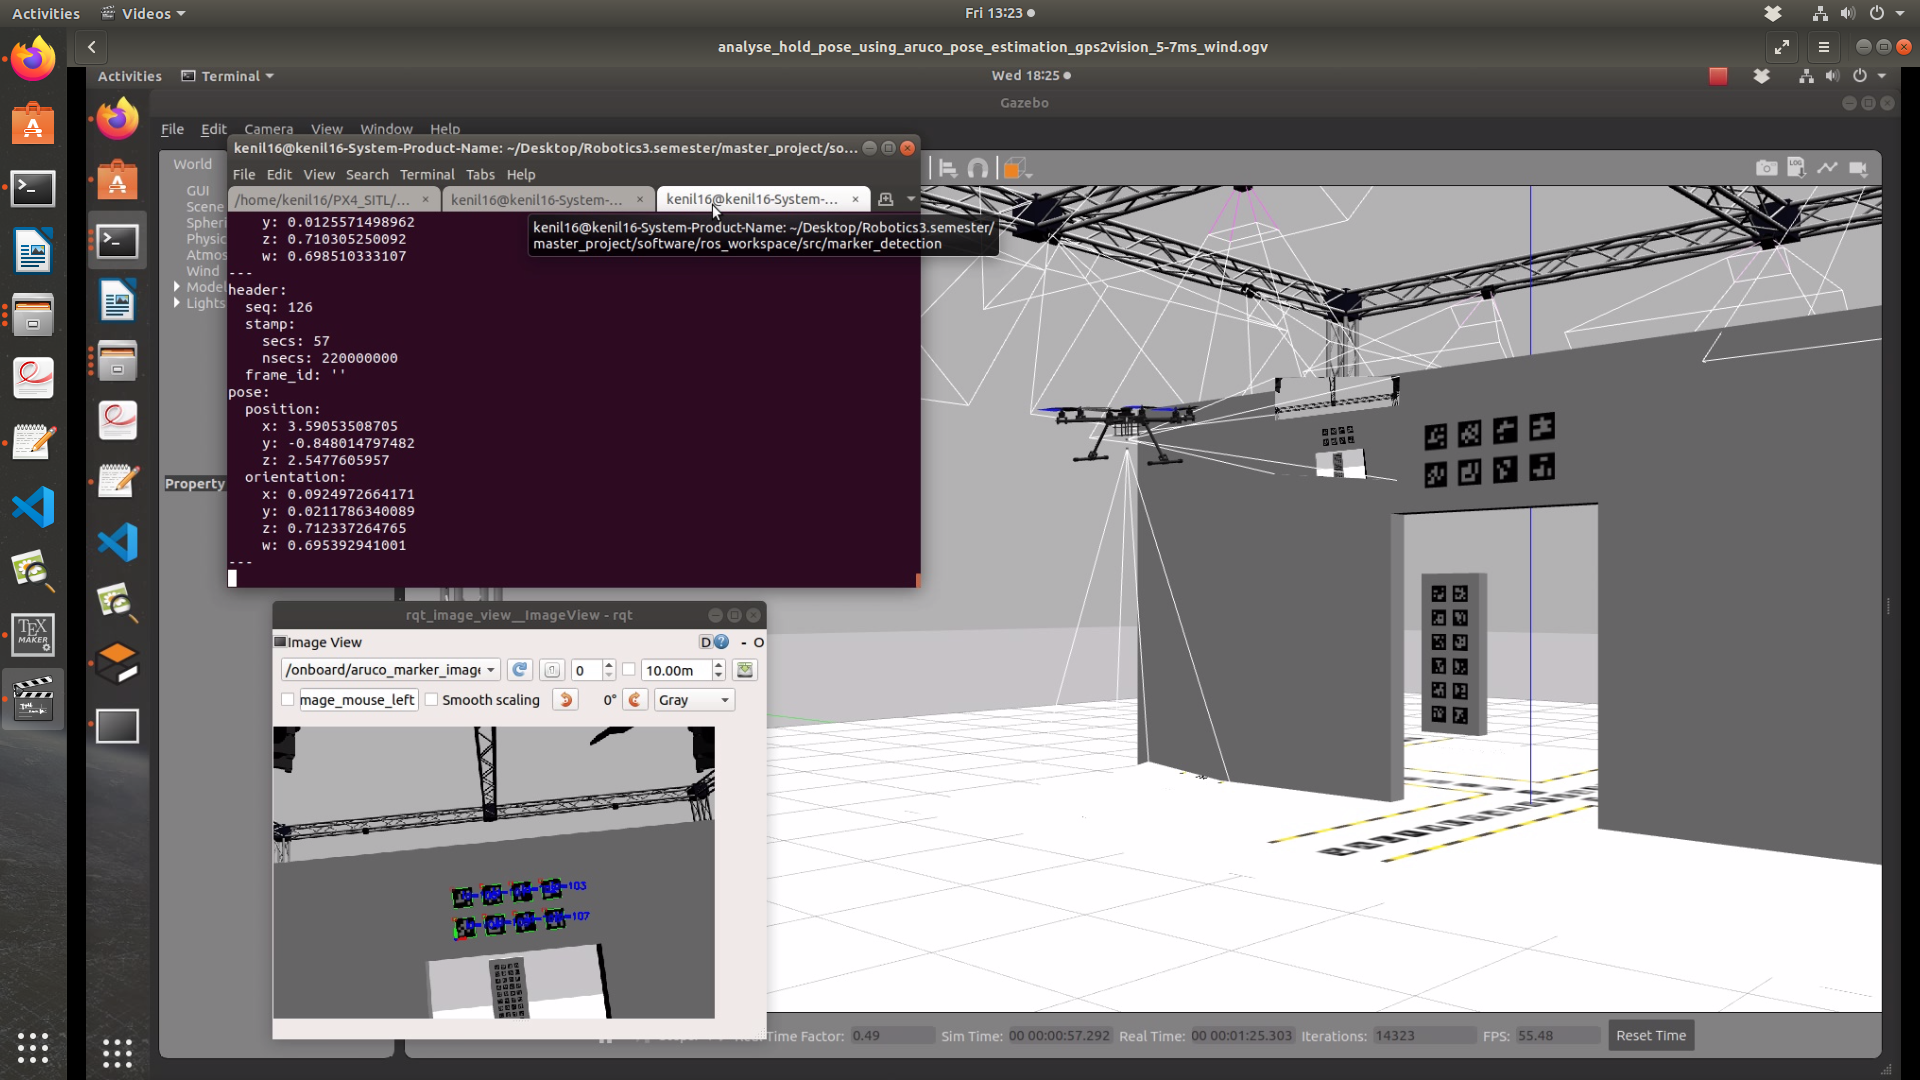
\includegraphics[width=\textwidth]{../Figures/hold_pose_using_aruco_pose_estimation/aruco_board_one_5-7ms_wind.png}
        \caption{}
        \label{fig:hold_pose_aruco_board_one_5-7ms_wind}
    \end{subfigure}
    \caption{}
    \label{fig:hold_pose_aruco_boards}
\end{figure}

\begin{table}[H]
    \centering
    \addtolength{\leftskip} {-2cm}
    \addtolength{\rightskip}{-2cm}
        \caption{Statistics of the results from landing tests }
        \pgfplotstabletypeset[normal,
                columns/eg/.style={
                column name={Runs},
                dec sep align
        }
        ]{ %
        Estimation error & eg & Wind & Mean position & STD position & Mean angle & STD angle\\
        \topmidheader{8}{\textbf{Test 1}}
ArUco pose         & 10      & No & $1.43cm$ & $1.10cm$ & $0.18^{\circ}$ & $0.13^{\circ}$\\
Setpoint         & 10      & No & $3.12cm $ & $2.58cm$ & $0.28^{\circ}$ & $0.22^{\circ}$\\
		\midheader{8}{\textbf{Test 2}}
ArUco pose         & 10      & Yes & $1.47cm $ & $0.95cm$ & $0.49^{\circ}$ & $0.31^{\circ}$\\
Setpoint         & 10      & Yes & $4.04cm $ & $3.35cm$ & $4.45^{\circ}$ & $1.49^{\circ}$\\
 }
\end{table}

\begin{table}[H]
    \centering
    \addtolength{\leftskip} {-2cm}
    \addtolength{\rightskip}{-2cm}
        \caption{Statistics of the results from landing tests }
        \pgfplotstabletypeset[normal,
                columns/eg/.style={
                column name={Runs},
                dec sep align
        }
        ]{ %
        Estimation error & eg & Wind & Mean position & STD position & Mean angle & STD angle\\
        \topmidheader{8}{\textbf{Test 3}}
ArUco pose         & 10      & No & $0.12cm $ & $0.23cm$ & $0.03^{\circ}$ & $0.05^{\circ}$\\
Setpoint         & 10      & No & $2.93cm$ & $2.90cm$ & $0.12^{\circ}$ & $0.12^{\circ}$\\
		\midheader{8}{\textbf{Test 4}}
ArUco pose         & 10      & No & $0.11cm $ & $0.21cm$ & $0.02^{\circ}$ & $0.01^{\circ}$\\
Setpoint         & 10      & No & $2.92cm$ & $2.89cm$ & $0.11^{\circ}$ & $0.09^{\circ}$\\
		\midheader{8}{\textbf{Test 5}}
ArUco pose         & 10      & No & $0.09cm $ & $0.20cm$ &
$0.02^{\circ}$ & $0.01^{\circ}$\\
Setpoint         & 10      & No & $2.89cm$ & $2.85cm$ & $0.11^{\circ}$ & $0.09^{\circ}$\\
 }
\end{table}


\begin{figure}[H]
    \centering
    \begin{subfigure}[t]{.30\textwidth}
        \centering
        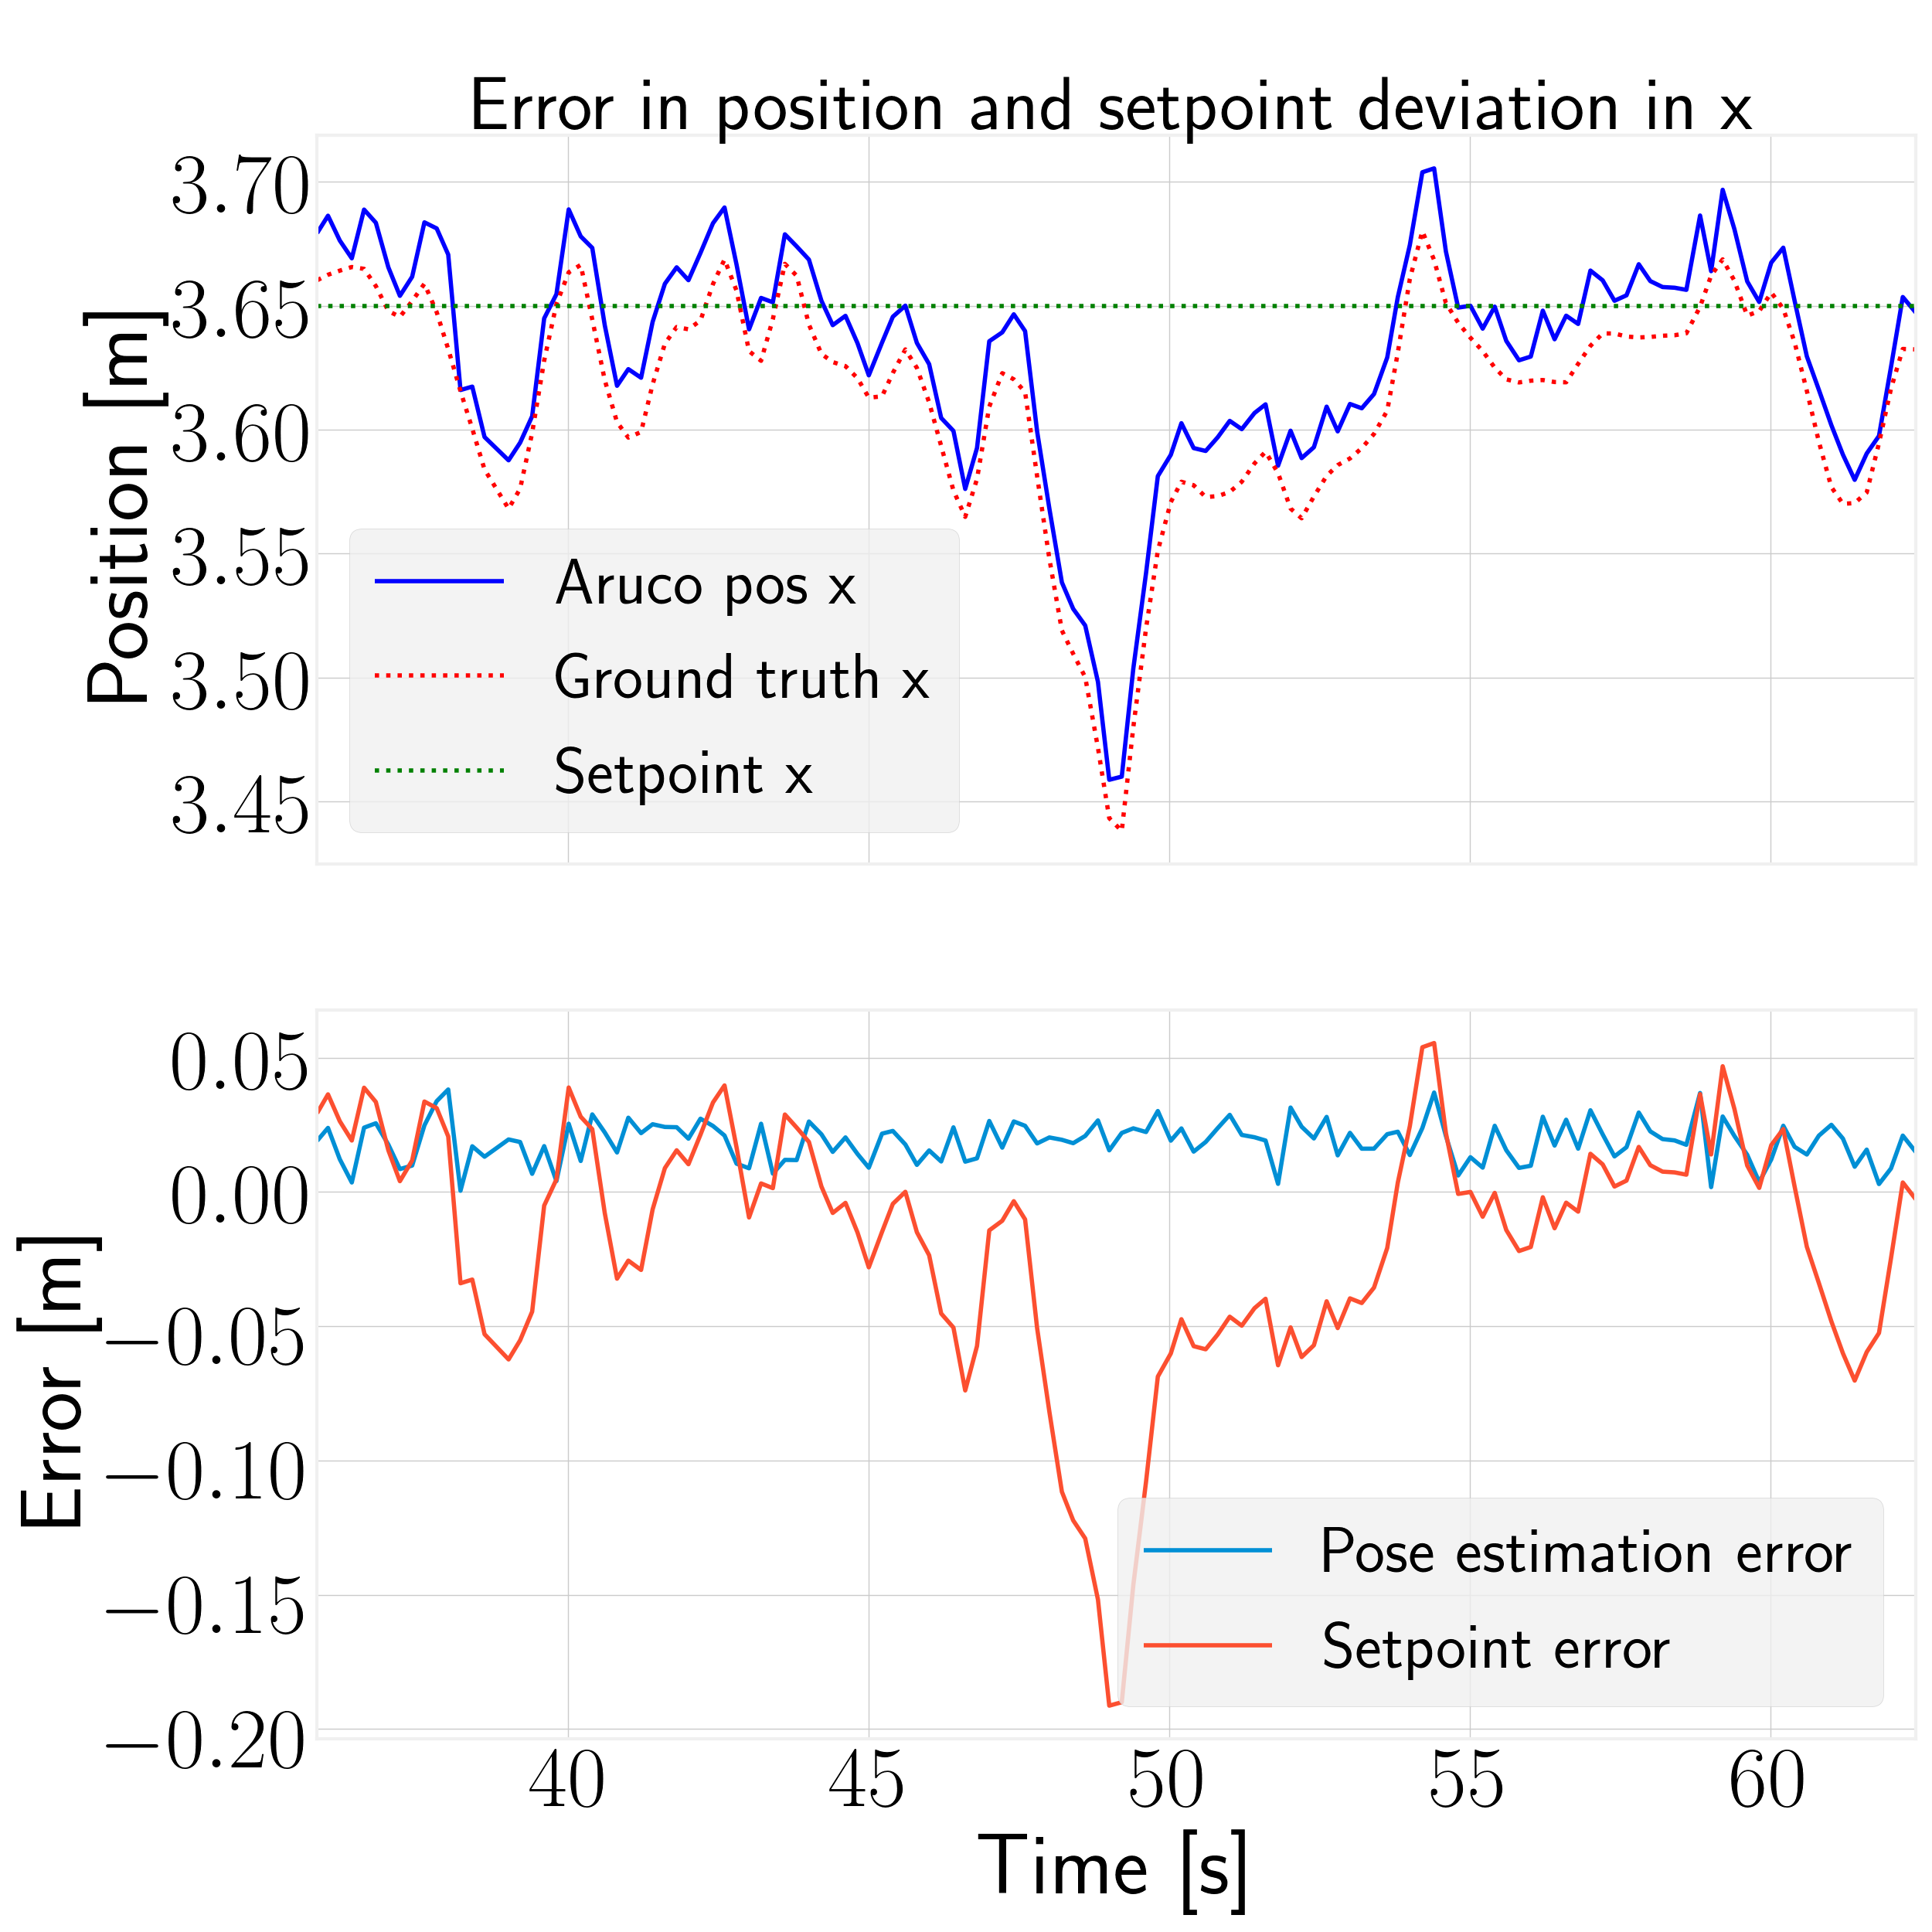
\includegraphics[width=\textwidth]{../Figures/hold_pose_using_aruco_pose_estimation/test2_gps2visionBoard_1.0Wind_-1.0y/error_x/pose_error_x_test1.png}
        \caption{}
        \label{fig:hold_pose_estimation_test2_x}
    \end{subfigure}
     \hspace{0.2em}
    \begin{subfigure}[t]{.30\textwidth}
        \centering
        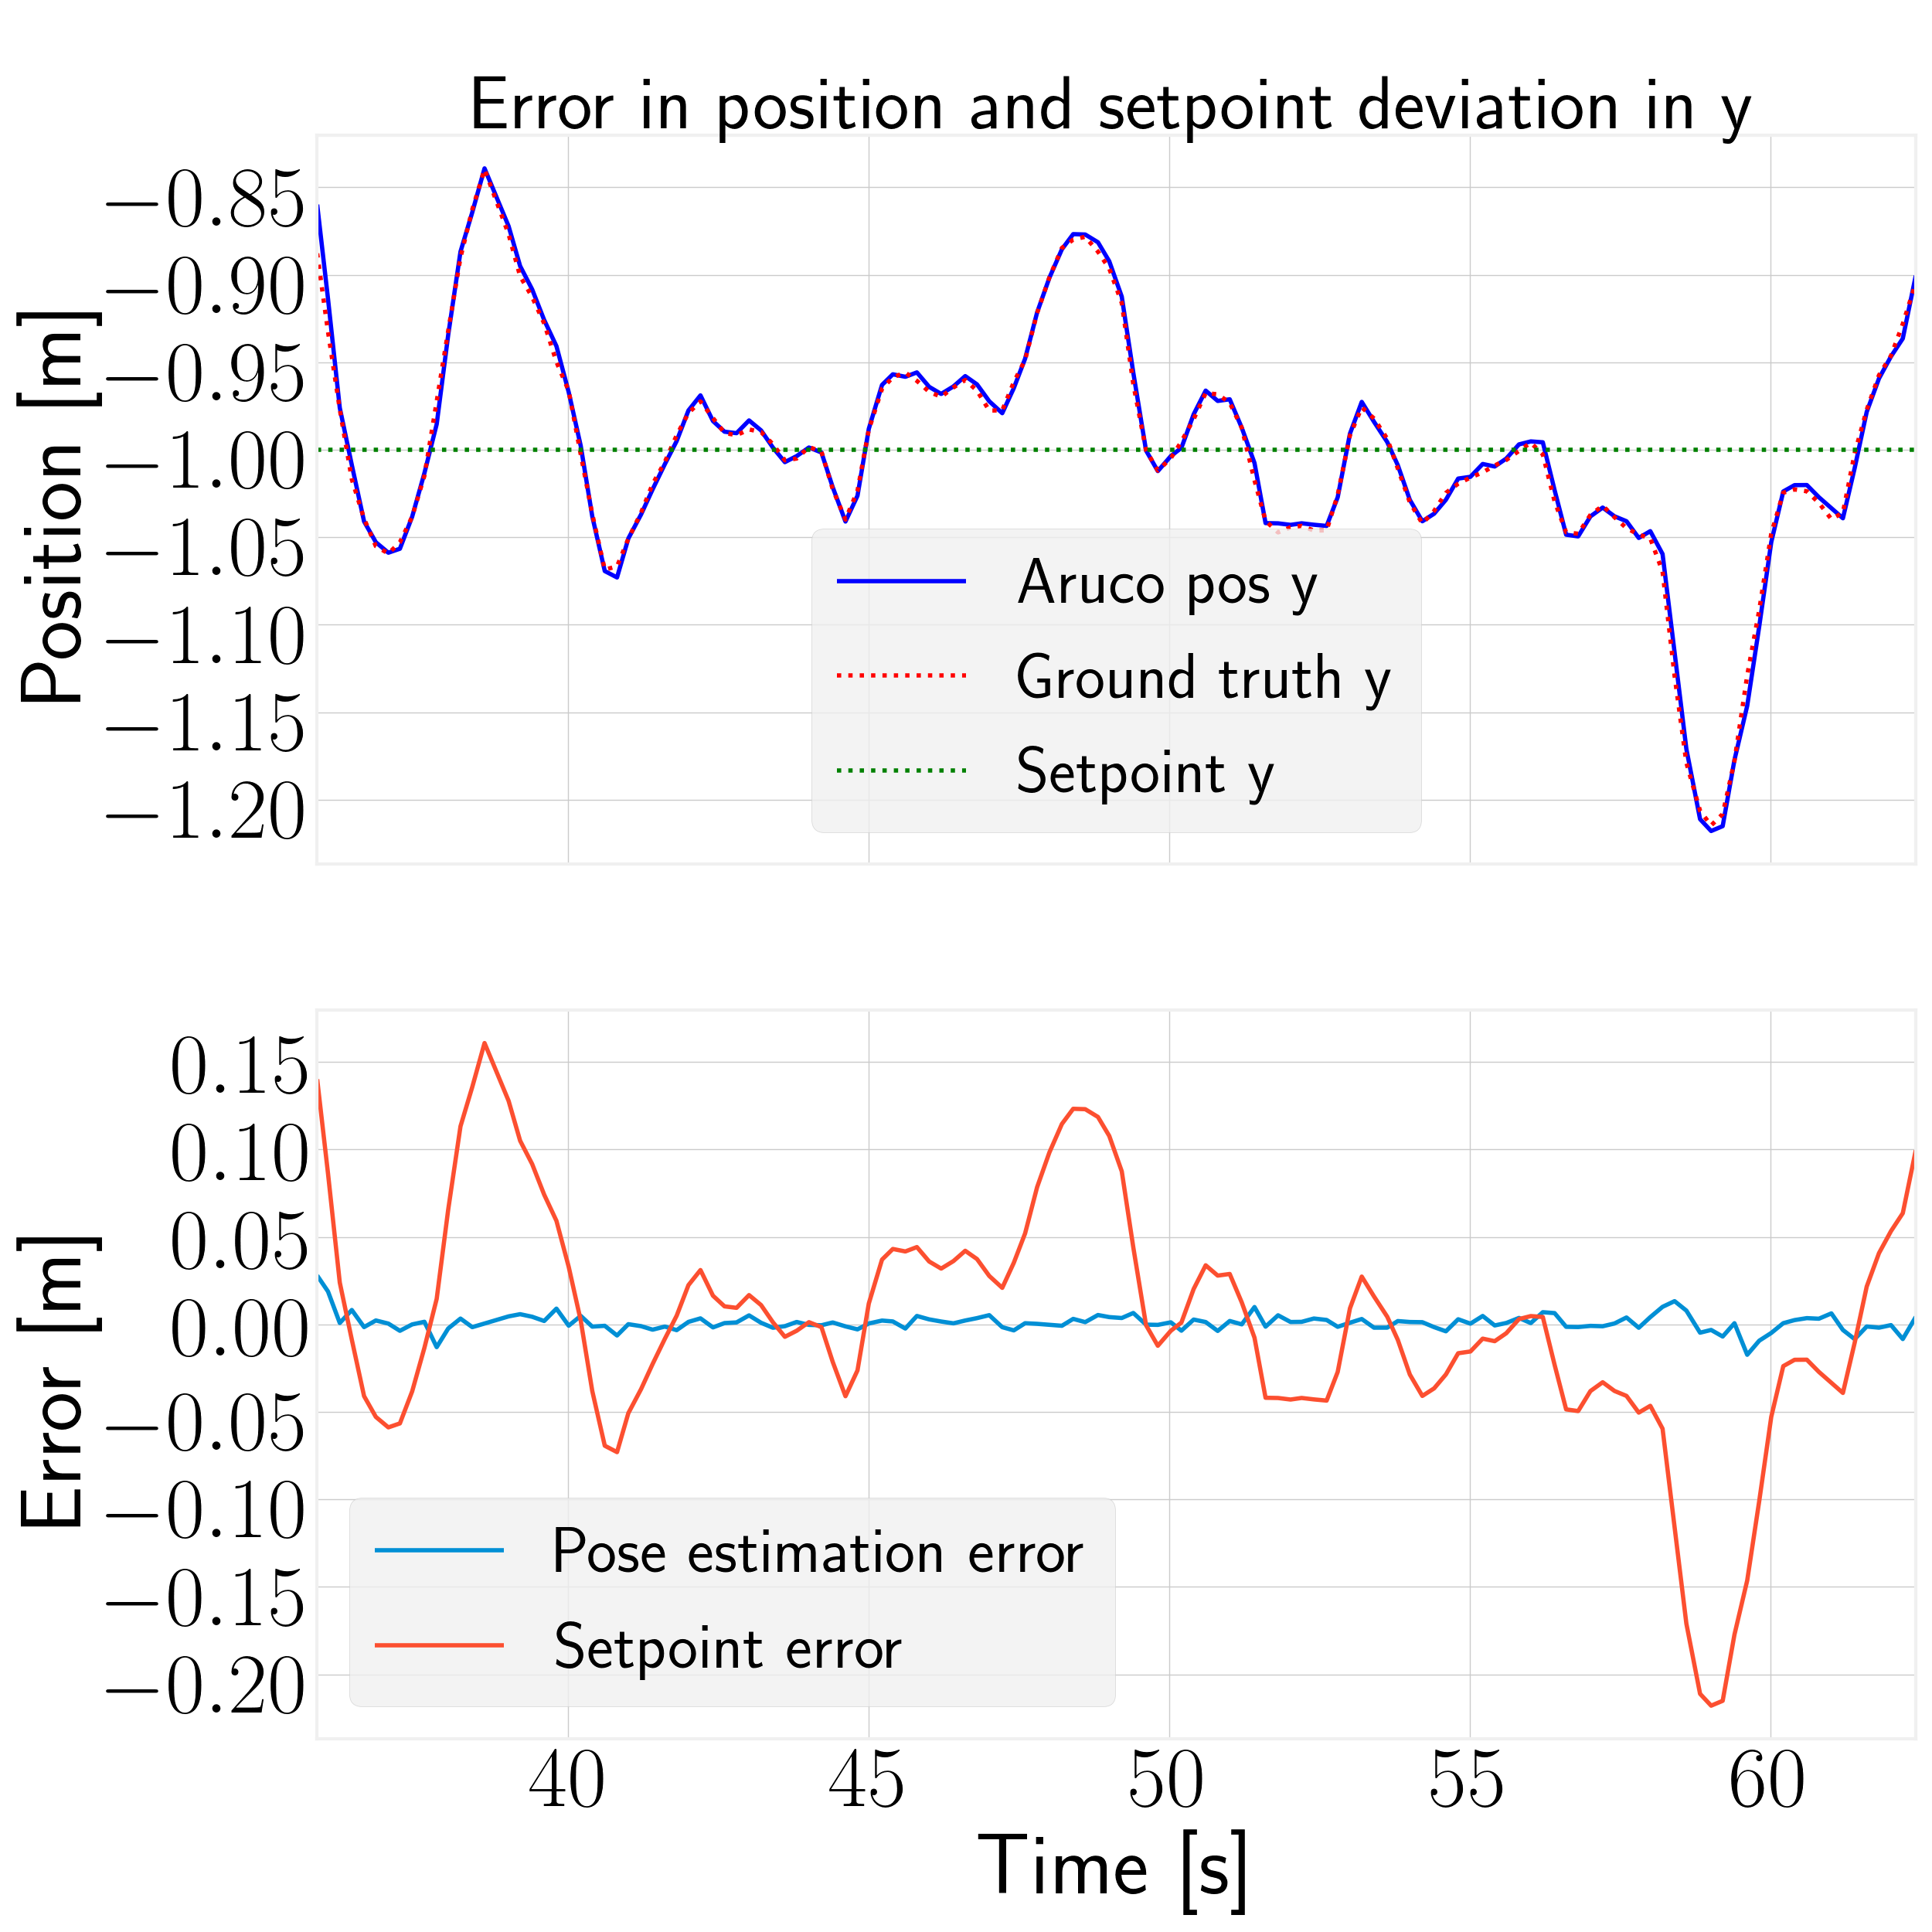
\includegraphics[width=\textwidth]{../Figures//hold_pose_using_aruco_pose_estimation/test2_gps2visionBoard_1.0Wind_-1.0y/error_y/pose_error_y_test1.png}
        \caption{}
        \label{fig:hold_pose_estimation_test2_y}
    \end{subfigure}
     \hspace{0.2em}
    \begin{subfigure}[t]{.30\textwidth}
        \centering
        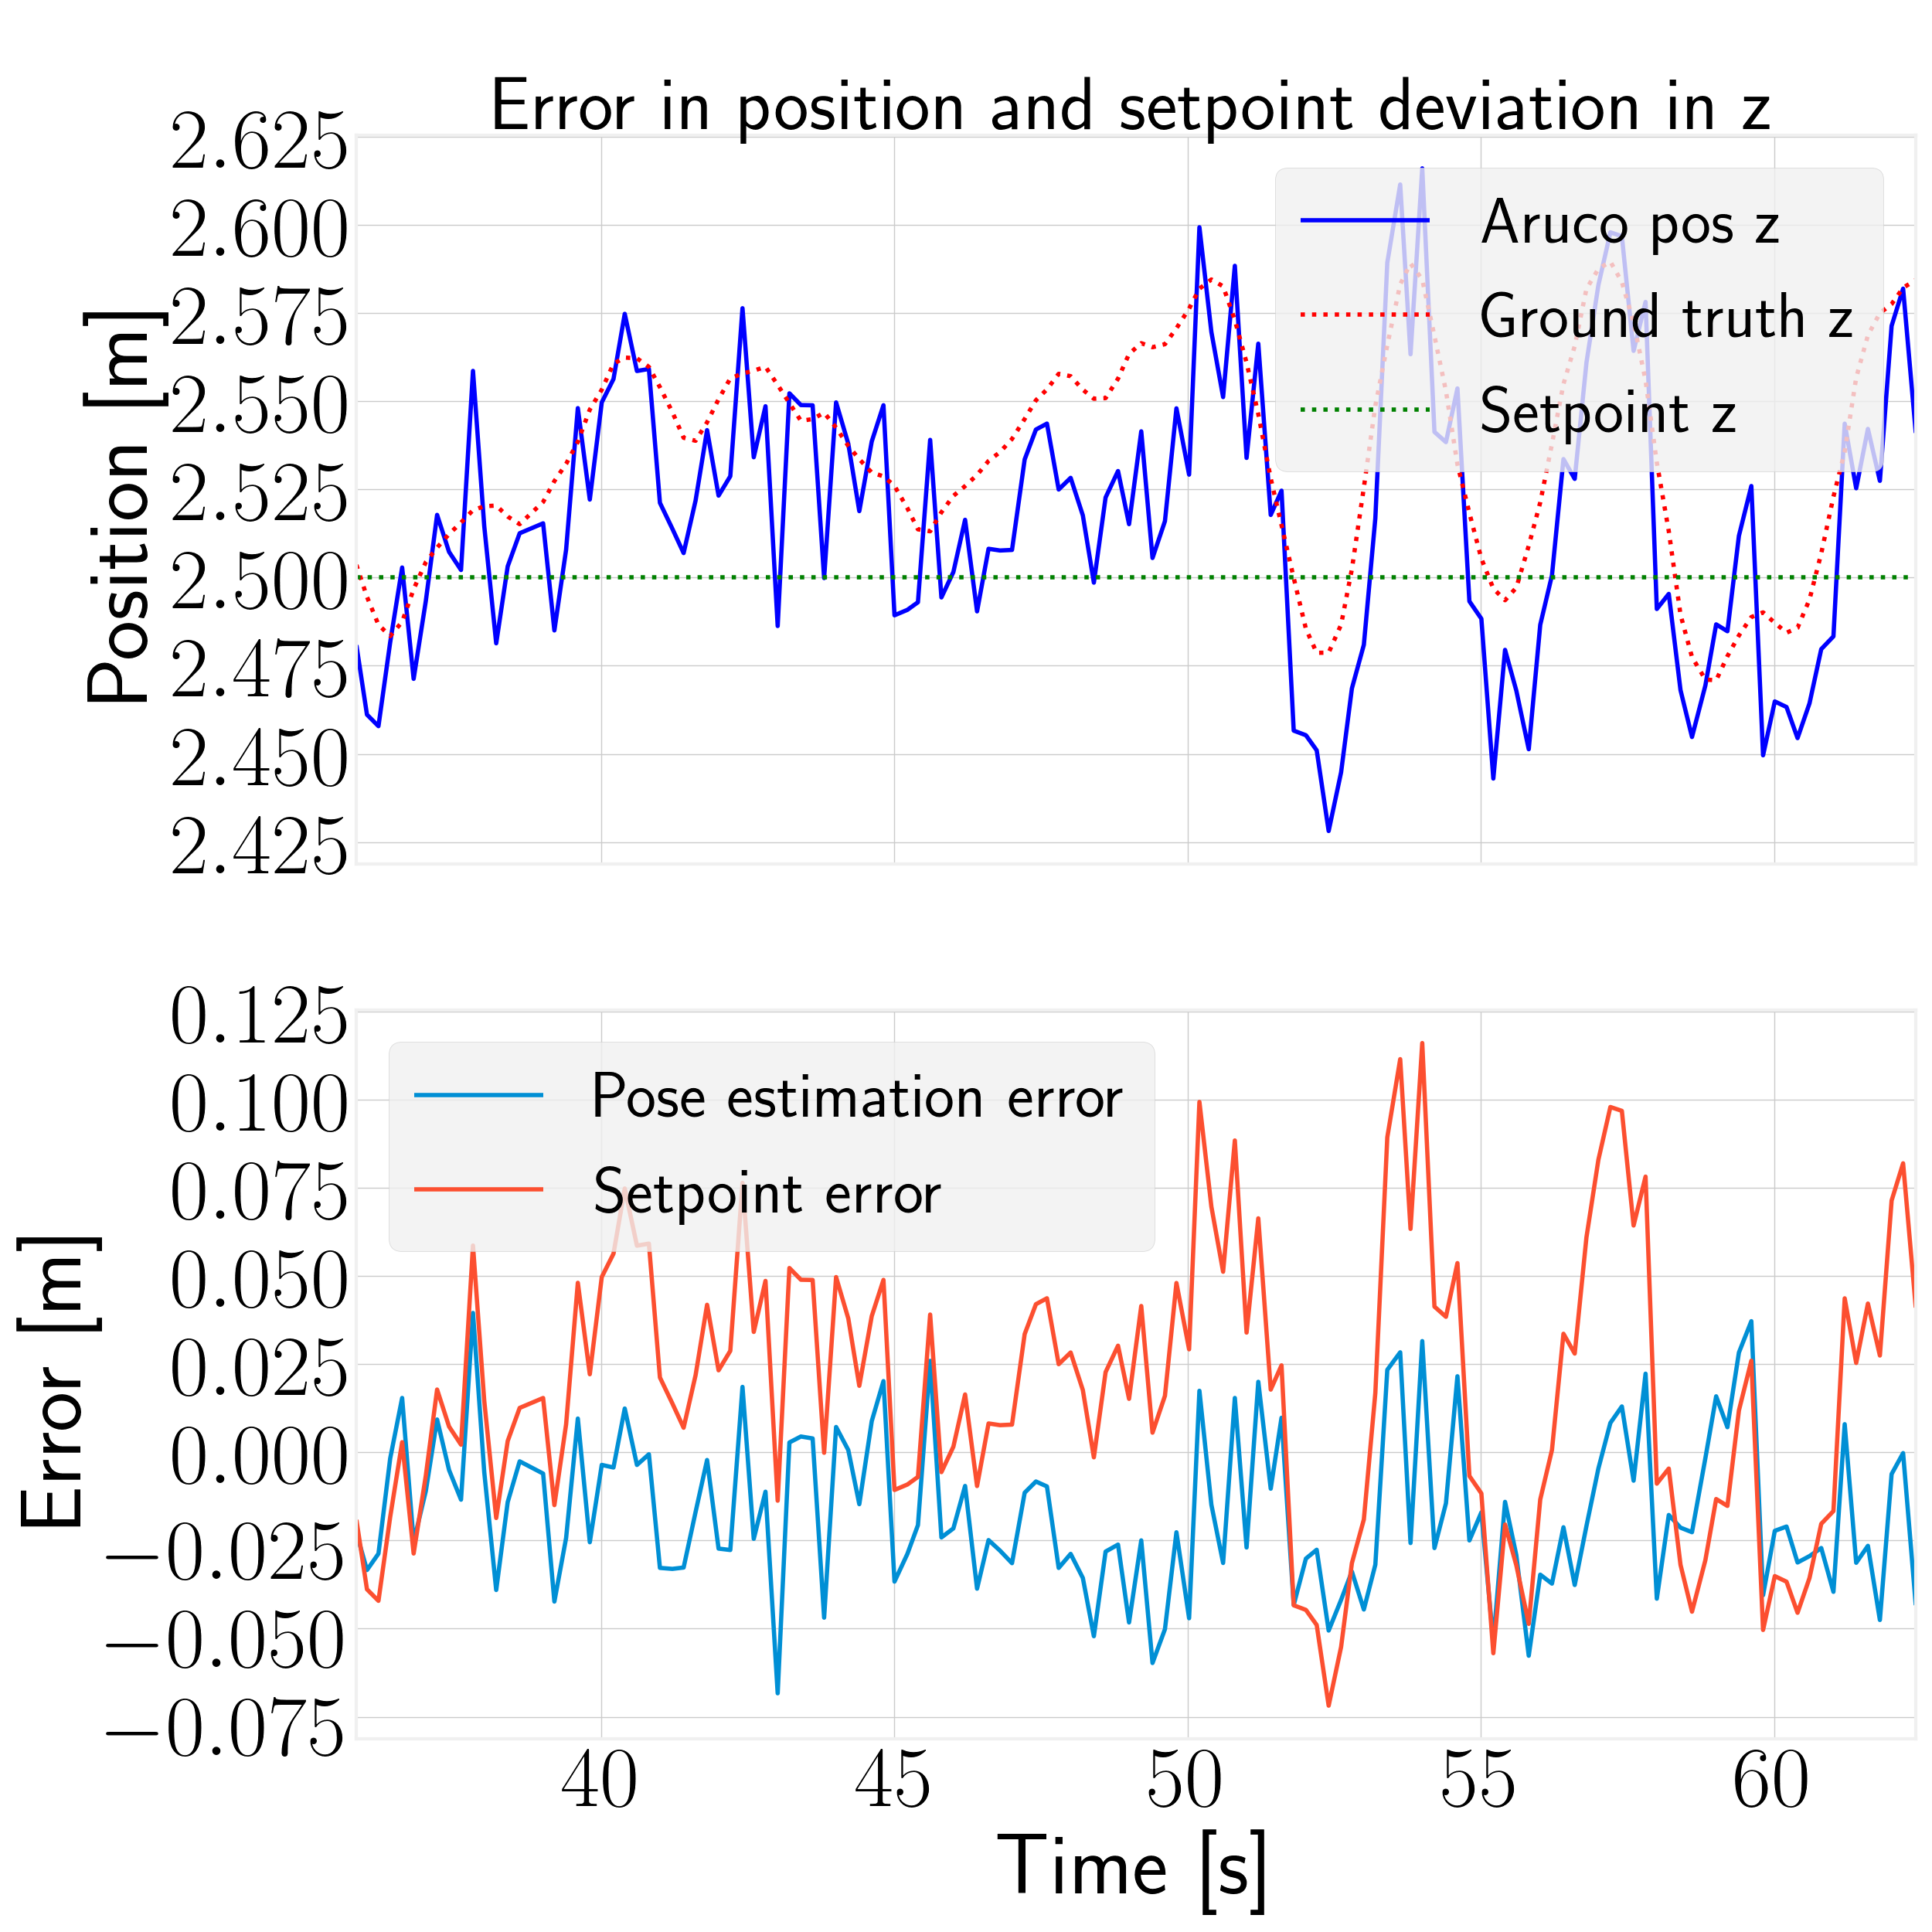
\includegraphics[width=\textwidth]{../Figures/hold_pose_using_aruco_pose_estimation/test2_gps2visionBoard_1.0Wind_-1.0y/error_z/pose_error_z_test1.png}
        \caption{}
        \label{fig:hold_pose_estimation_test2_z}
    \end{subfigure}
    \caption{}
    \label{fig:hold_pose_estimation_test2_error_pos}
\end{figure}

\begin{figure}[H]
    \centering
    \begin{subfigure}[t]{.30\textwidth}
        \centering
        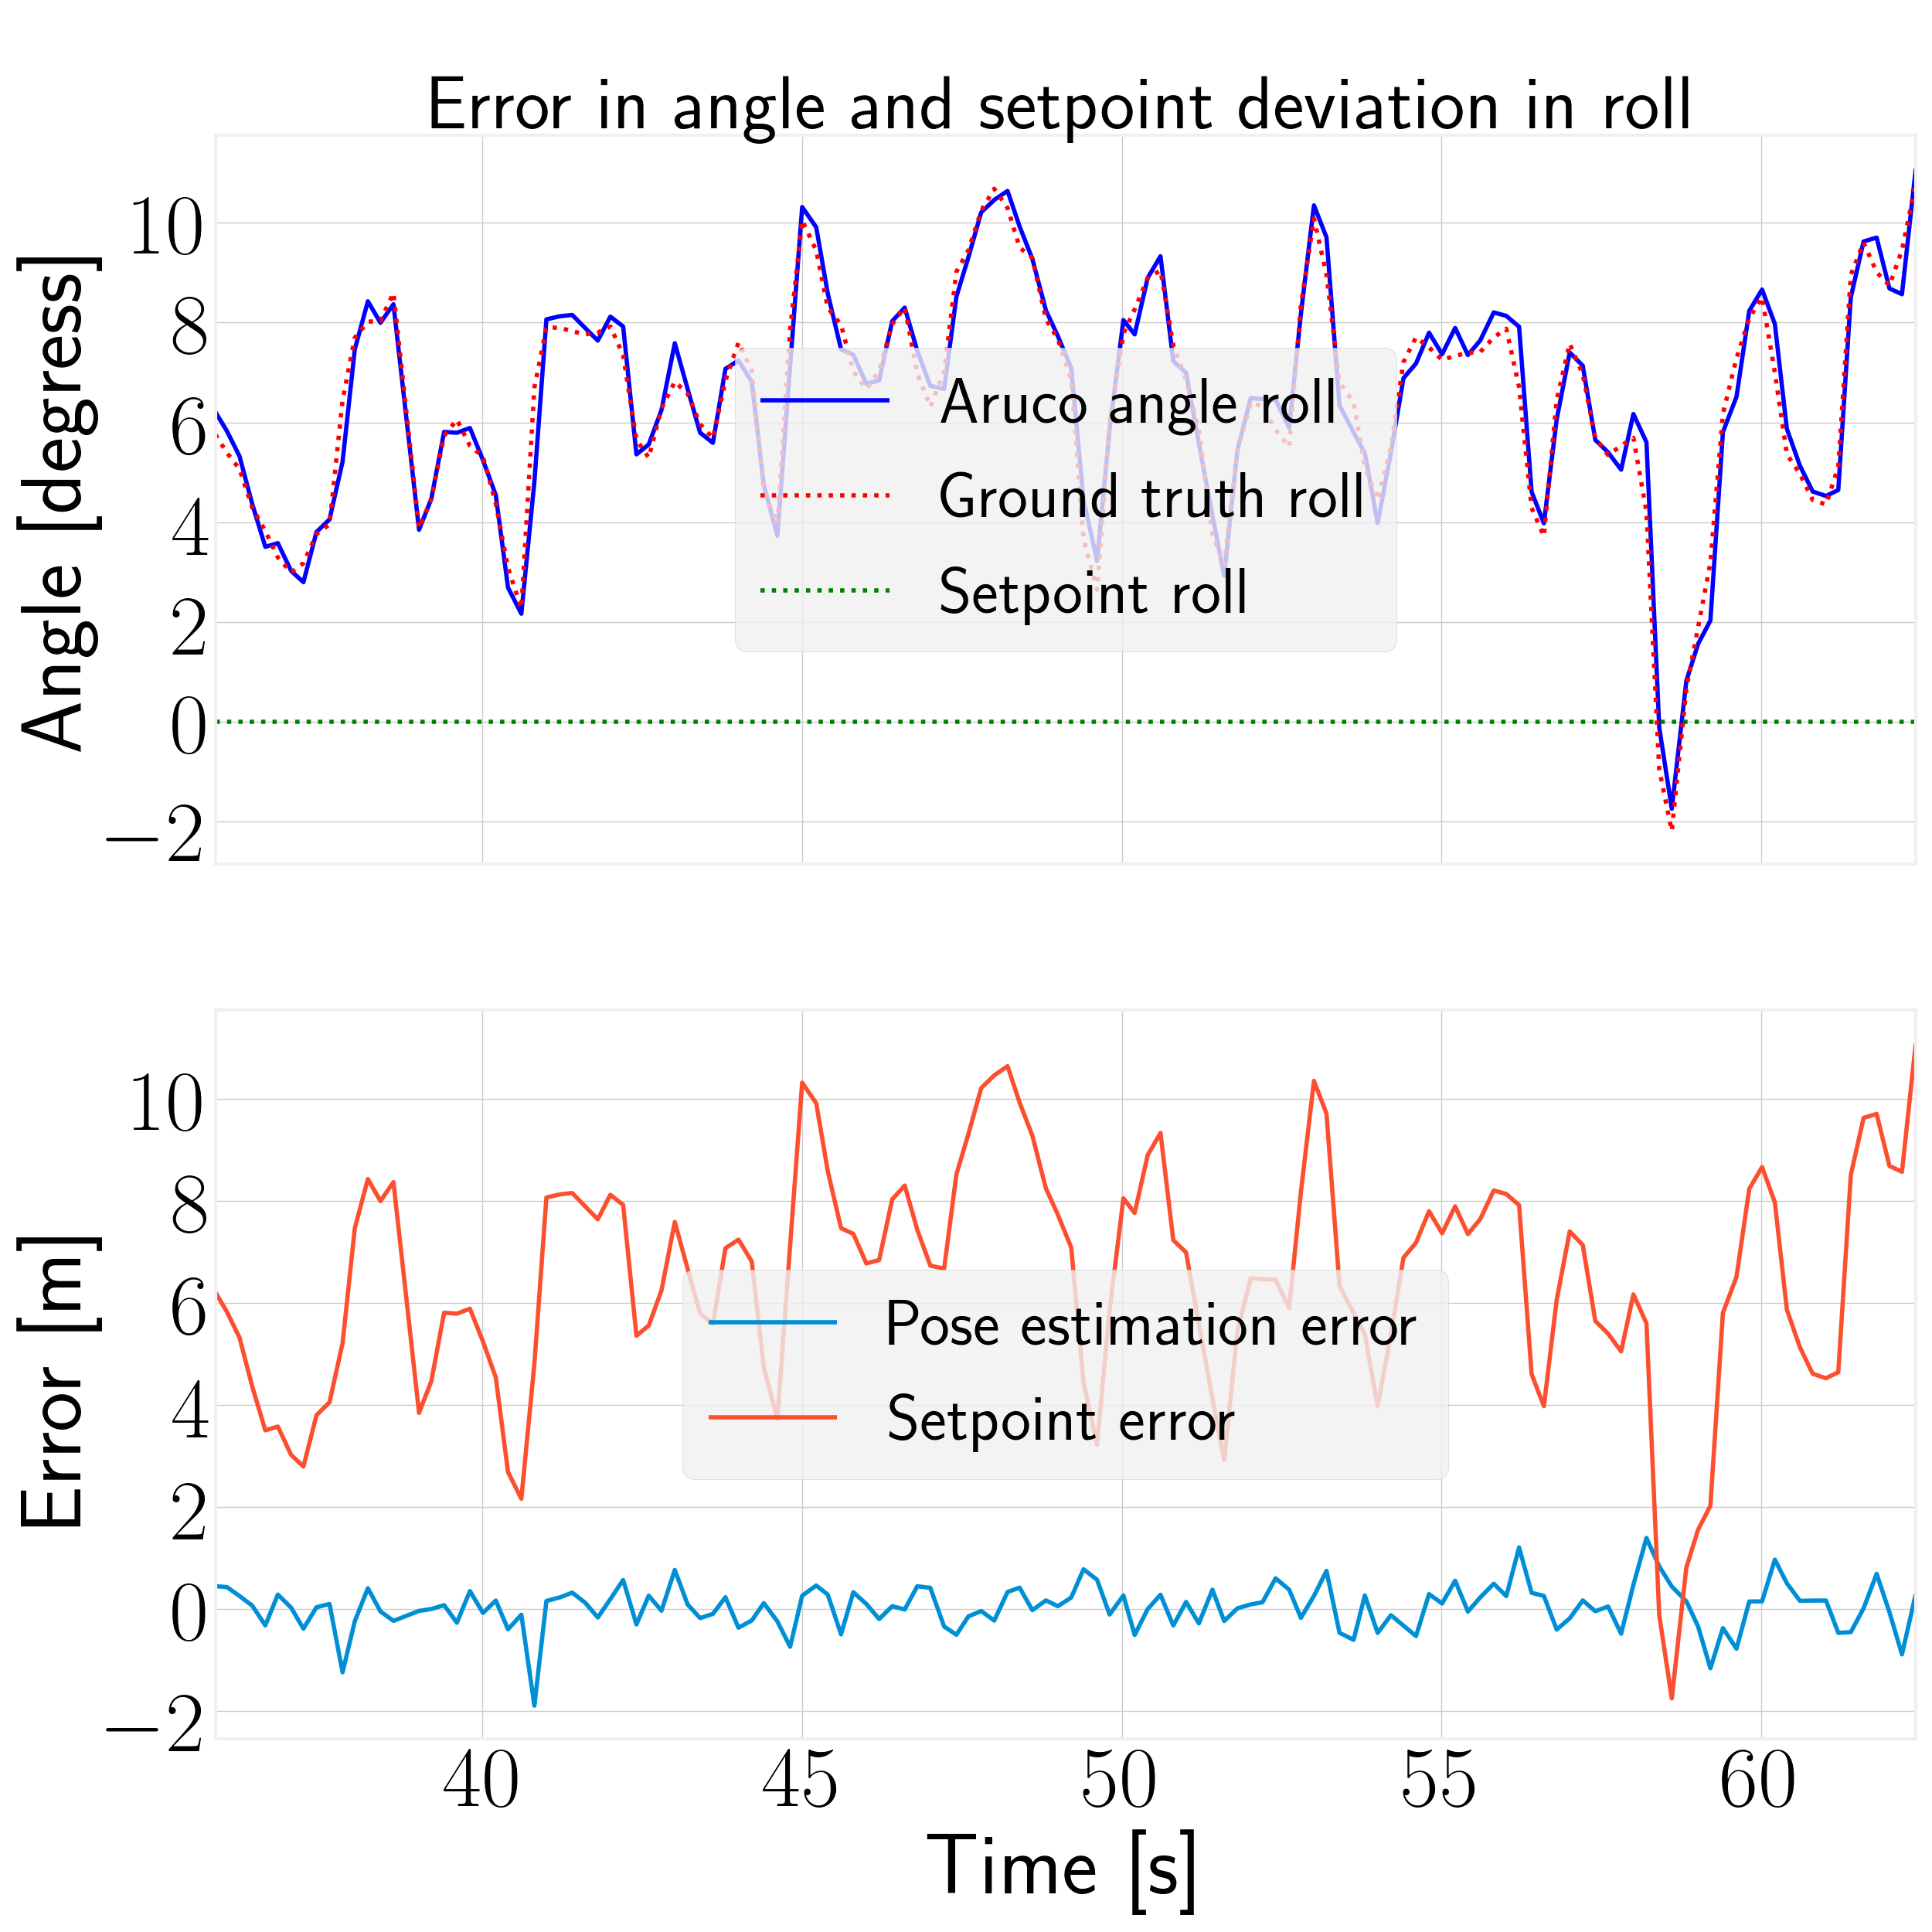
\includegraphics[width=\textwidth]{../Figures/hold_pose_using_aruco_pose_estimation/test2_gps2visionBoard_1.0Wind_-1.0y/error_roll/pose_error_roll_test1.png}
        \caption{}
        \label{fig:hold_pose_estimation_test2_roll}
    \end{subfigure}
     \hspace{0.2em}
    \begin{subfigure}[t]{.30\textwidth}
        \centering
        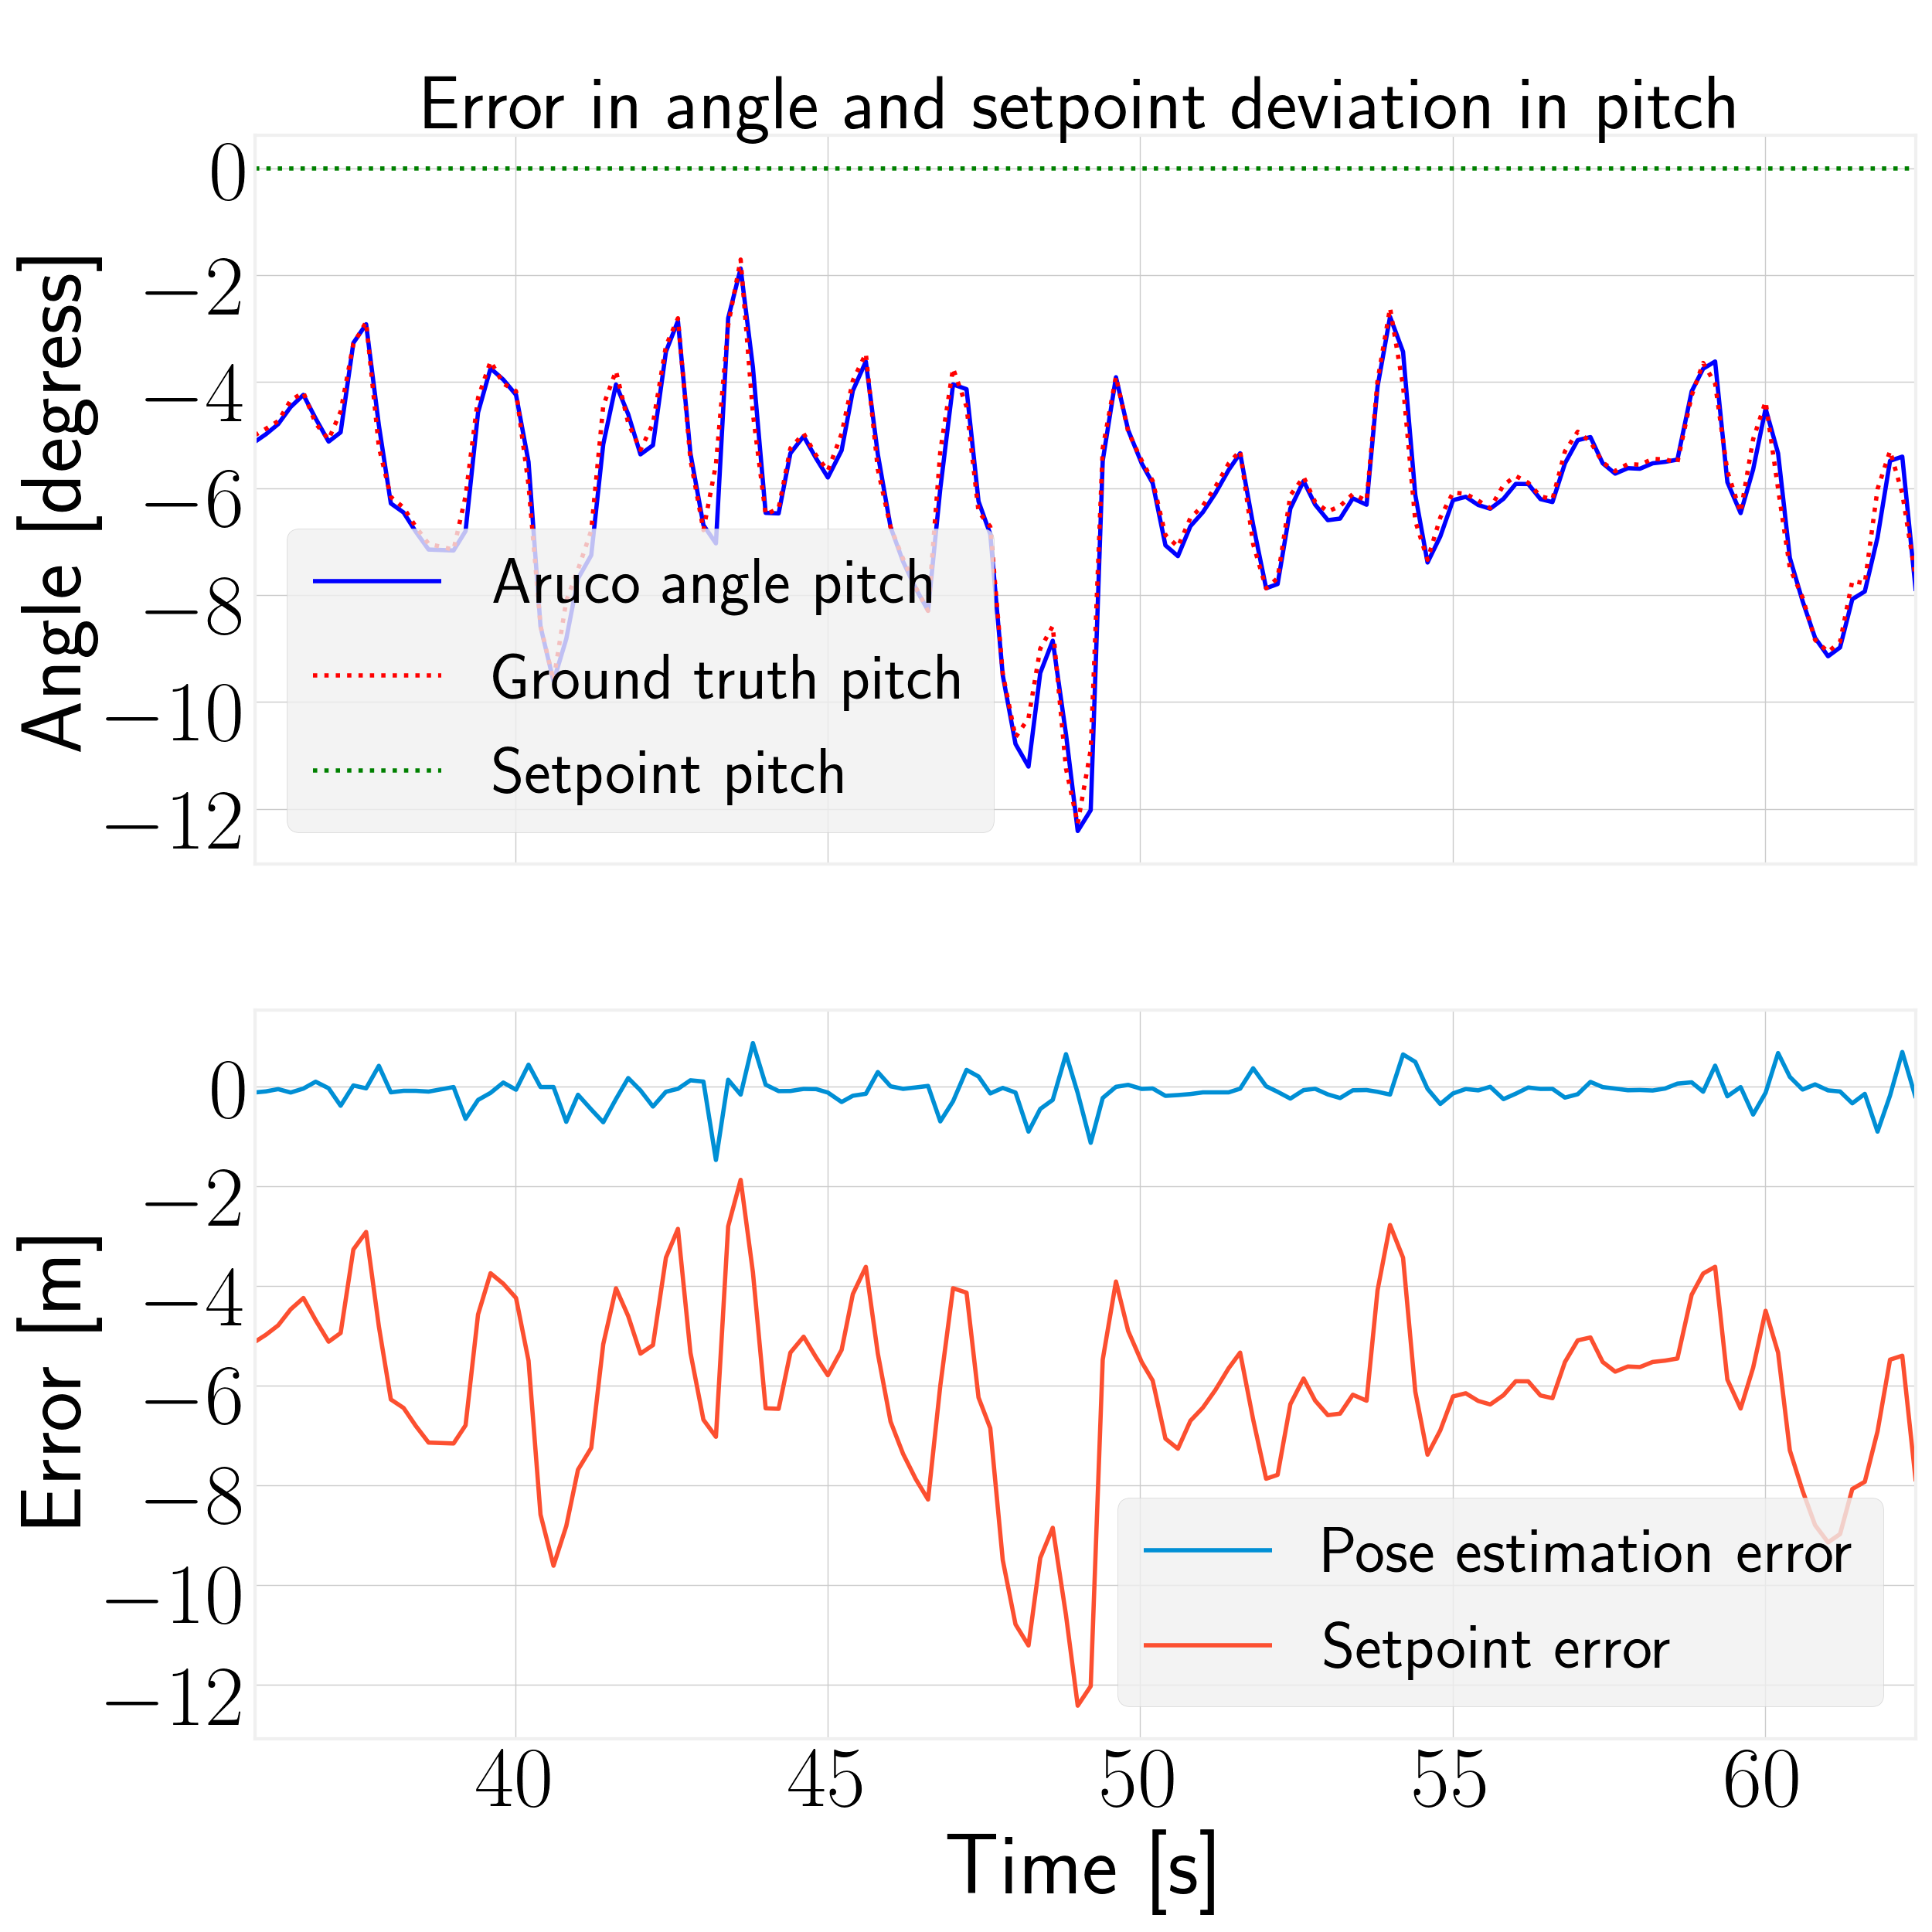
\includegraphics[width=\textwidth]{../Figures//hold_pose_using_aruco_pose_estimation/test2_gps2visionBoard_1.0Wind_-1.0y/error_pitch/pose_error_pitch_test1.png}
        \caption{}
        \label{fig:hold_pose_estimation_test2_pitch}
    \end{subfigure}
     \hspace{0.2em}
    \begin{subfigure}[t]{.30\textwidth}
        \centering
        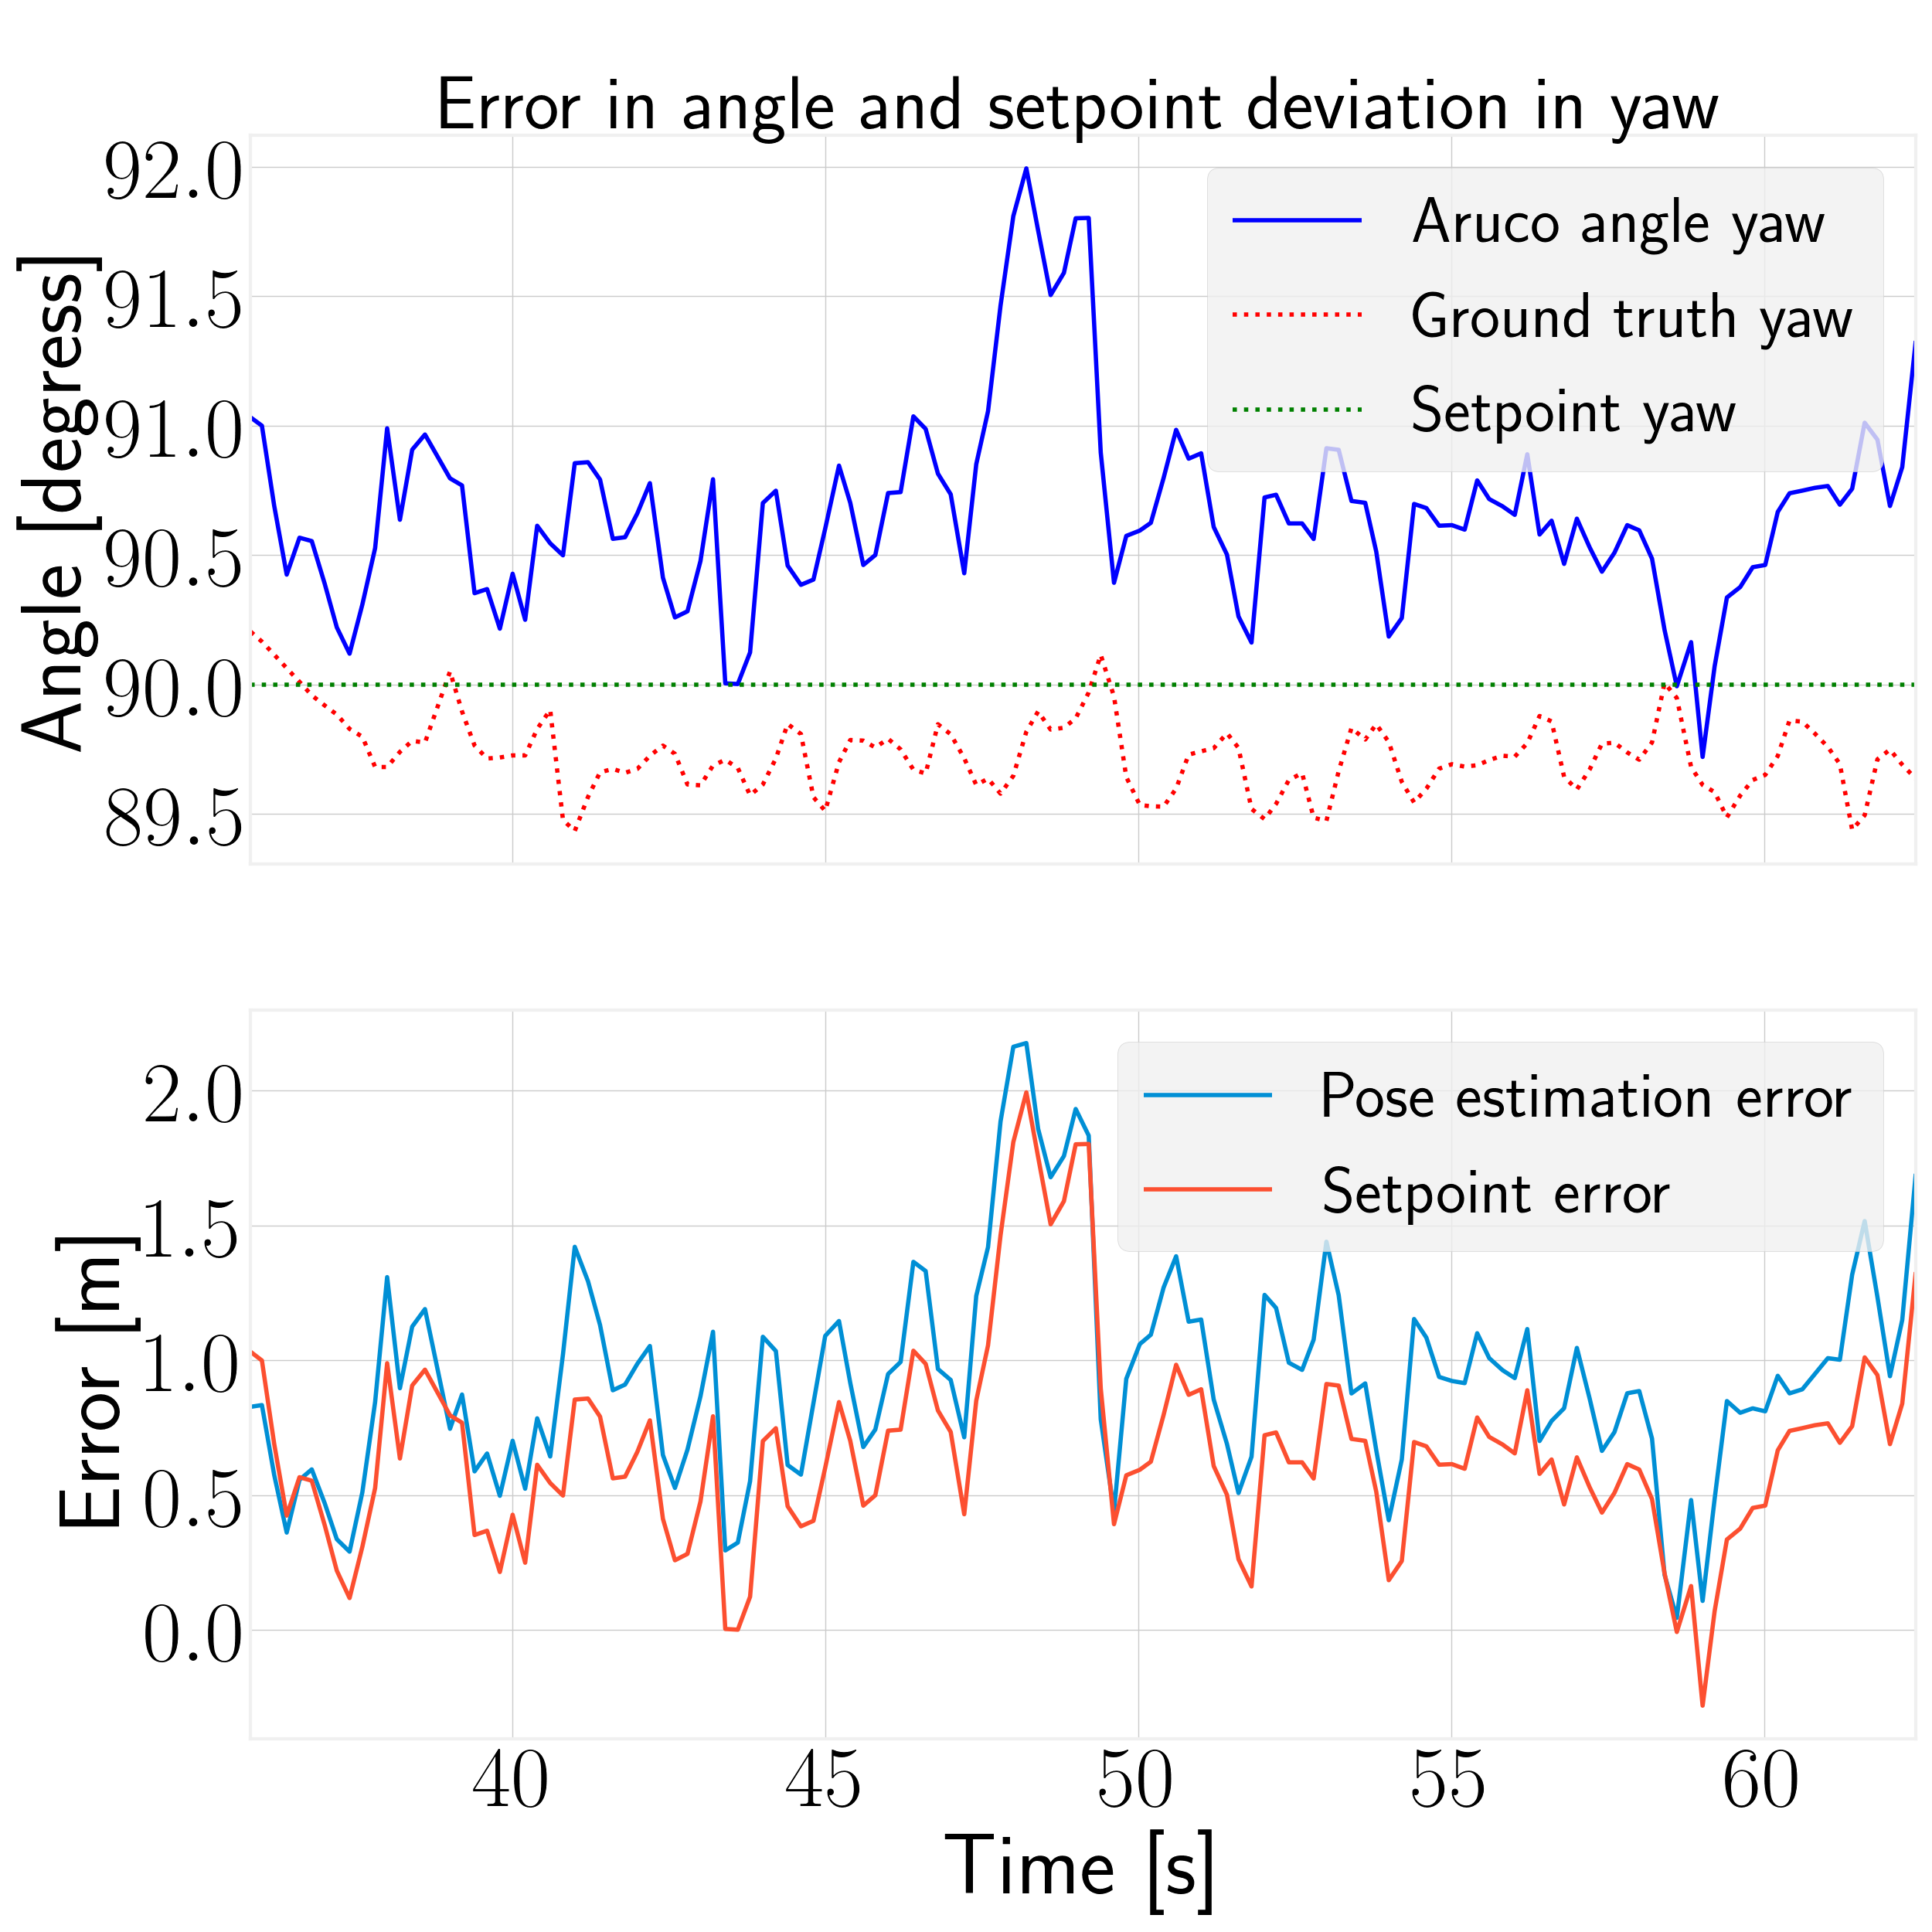
\includegraphics[width=\textwidth]{../Figures/hold_pose_using_aruco_pose_estimation/test2_gps2visionBoard_1.0Wind_-1.0y/error_yaw/pose_error_yaw_test1.png}
        \caption{}
        \label{fig:hold_pose_estimation_test2_yaw}
    \end{subfigure}
    \caption{}
    \label{fig:hold_pose_estimation_test2_error_angle}
\end{figure}

\begin{figure}[H]
    \centering
    \begin{subfigure}[t]{.30\textwidth}
        \centering
        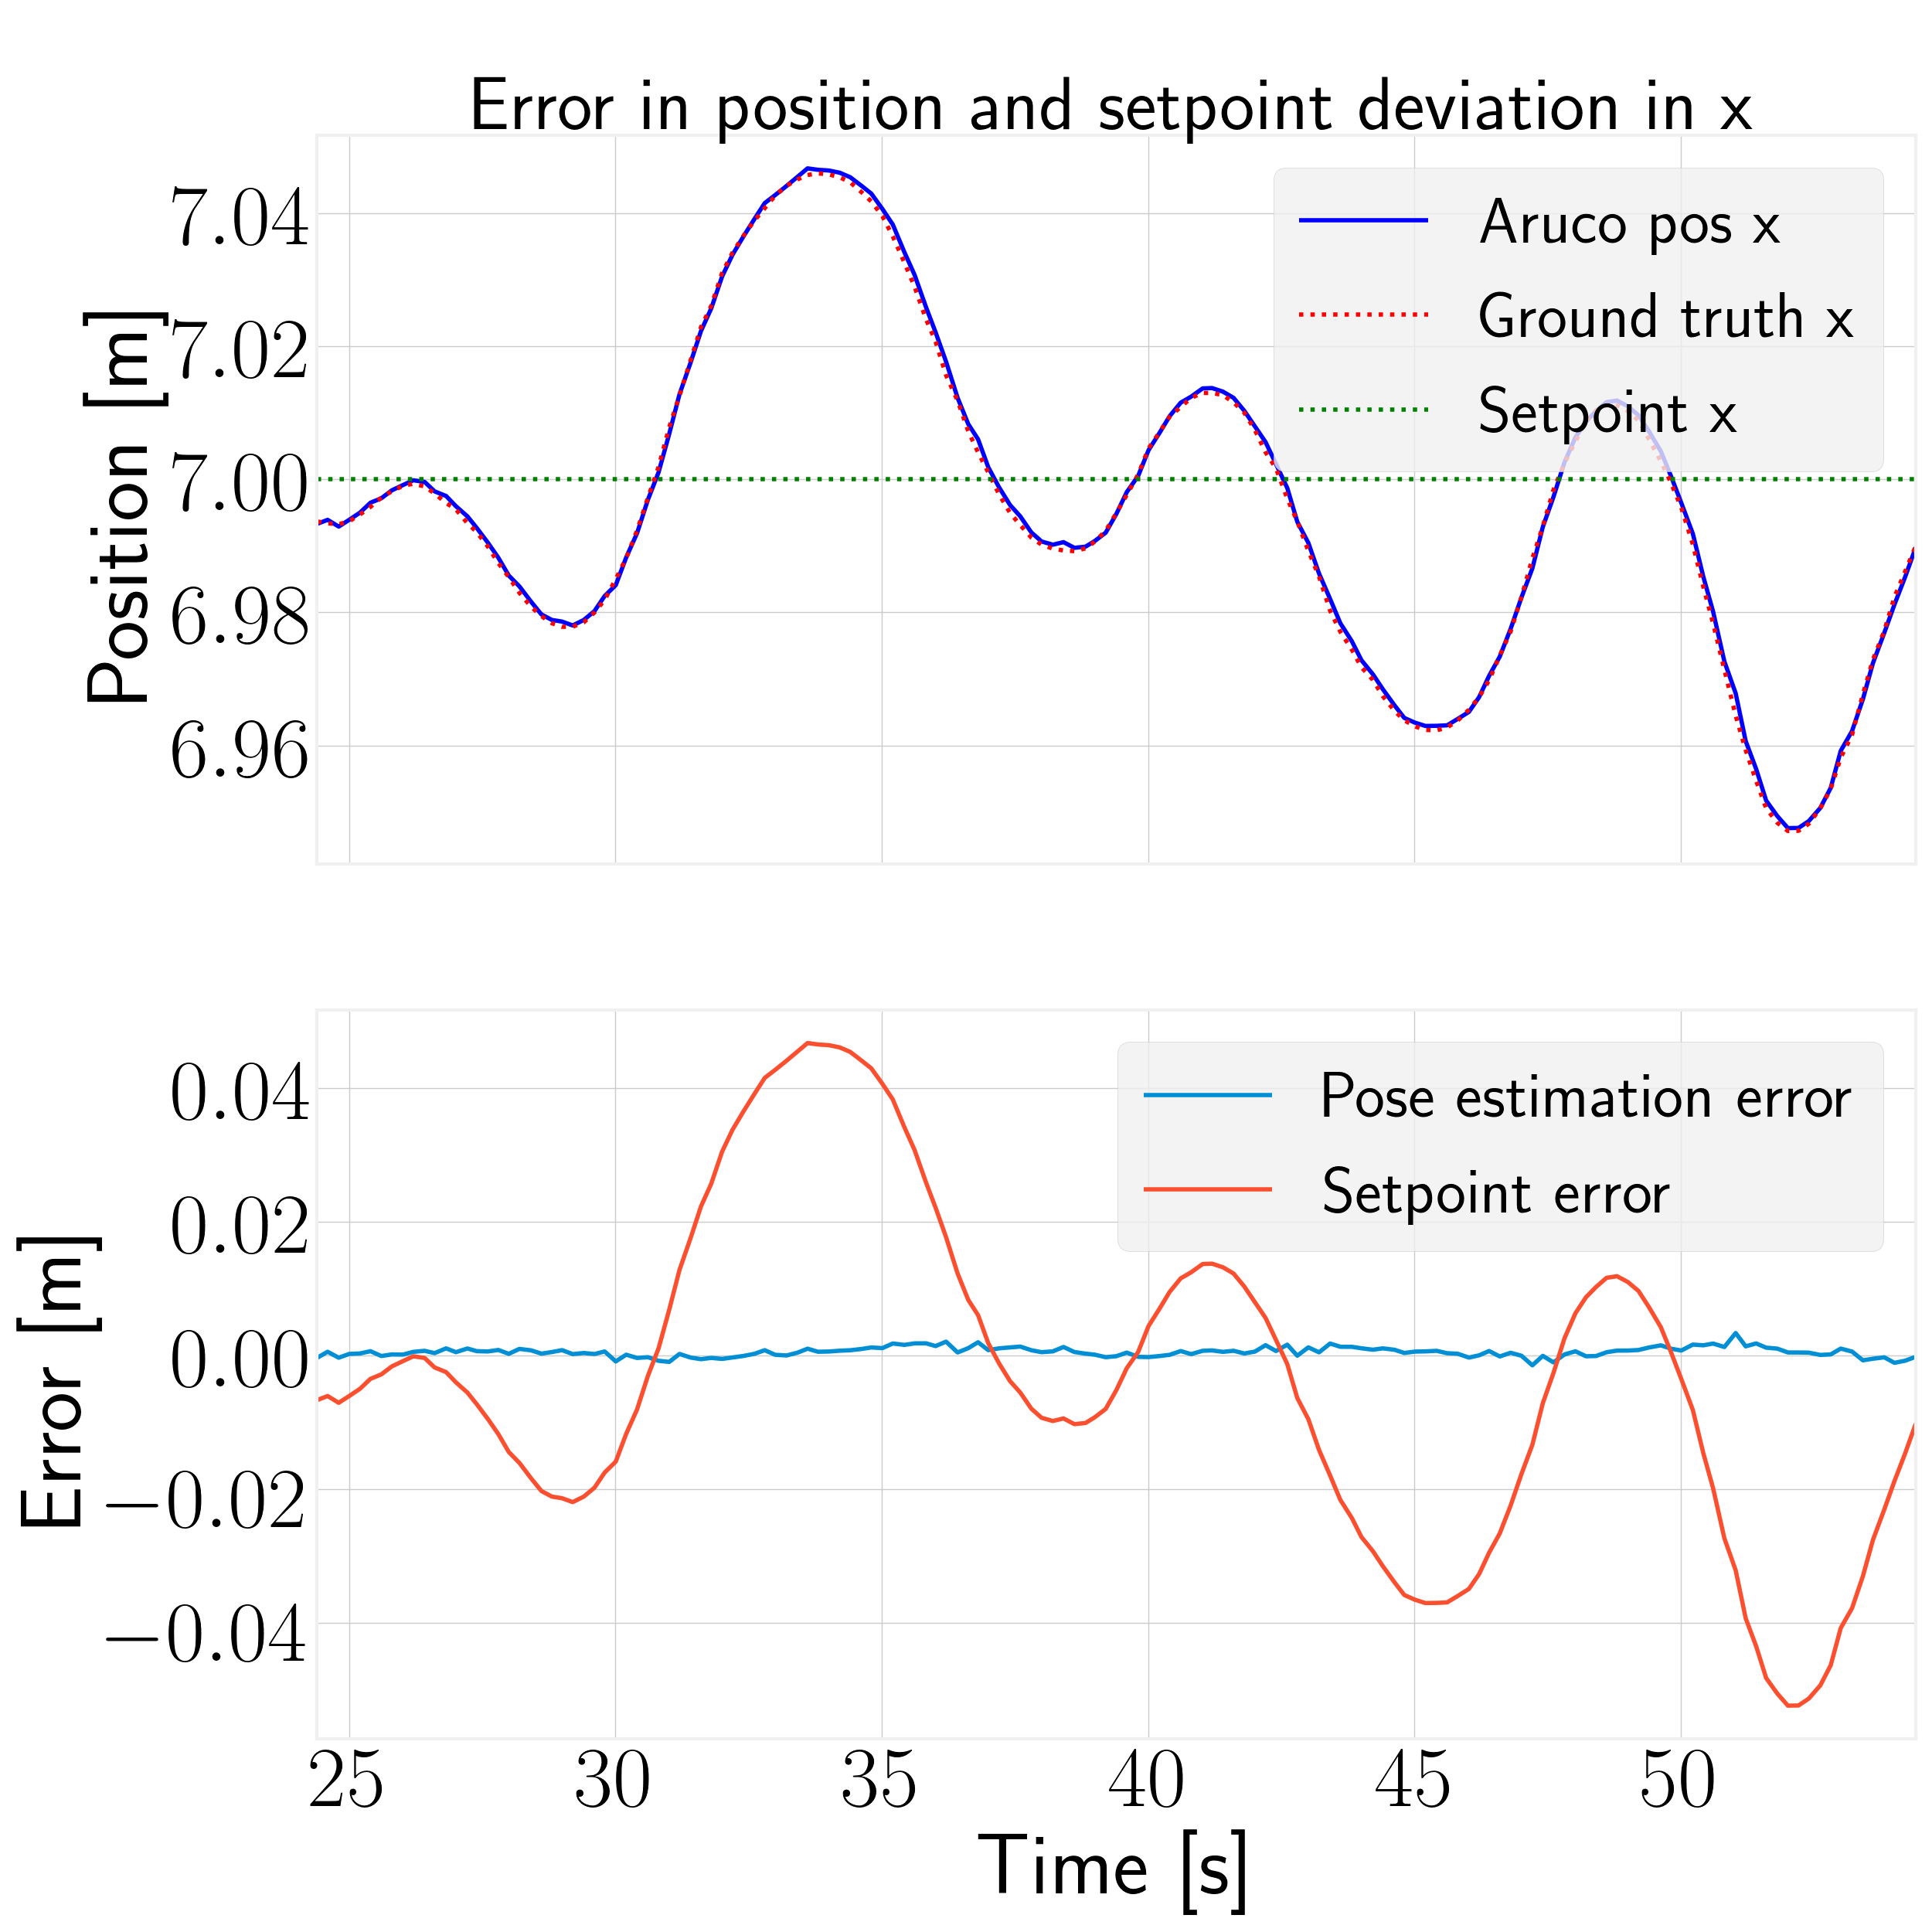
\includegraphics[width=\textwidth]{../Figures/hold_pose_using_aruco_pose_estimation/test5_landingBoard3_noWind/error_x/pose_error_x_test1.png}
        \caption{}
        \label{fig:hold_pose_estimation_test5_x}
    \end{subfigure}
     \hspace{0.2em}
    \begin{subfigure}[t]{.30\textwidth}
        \centering
        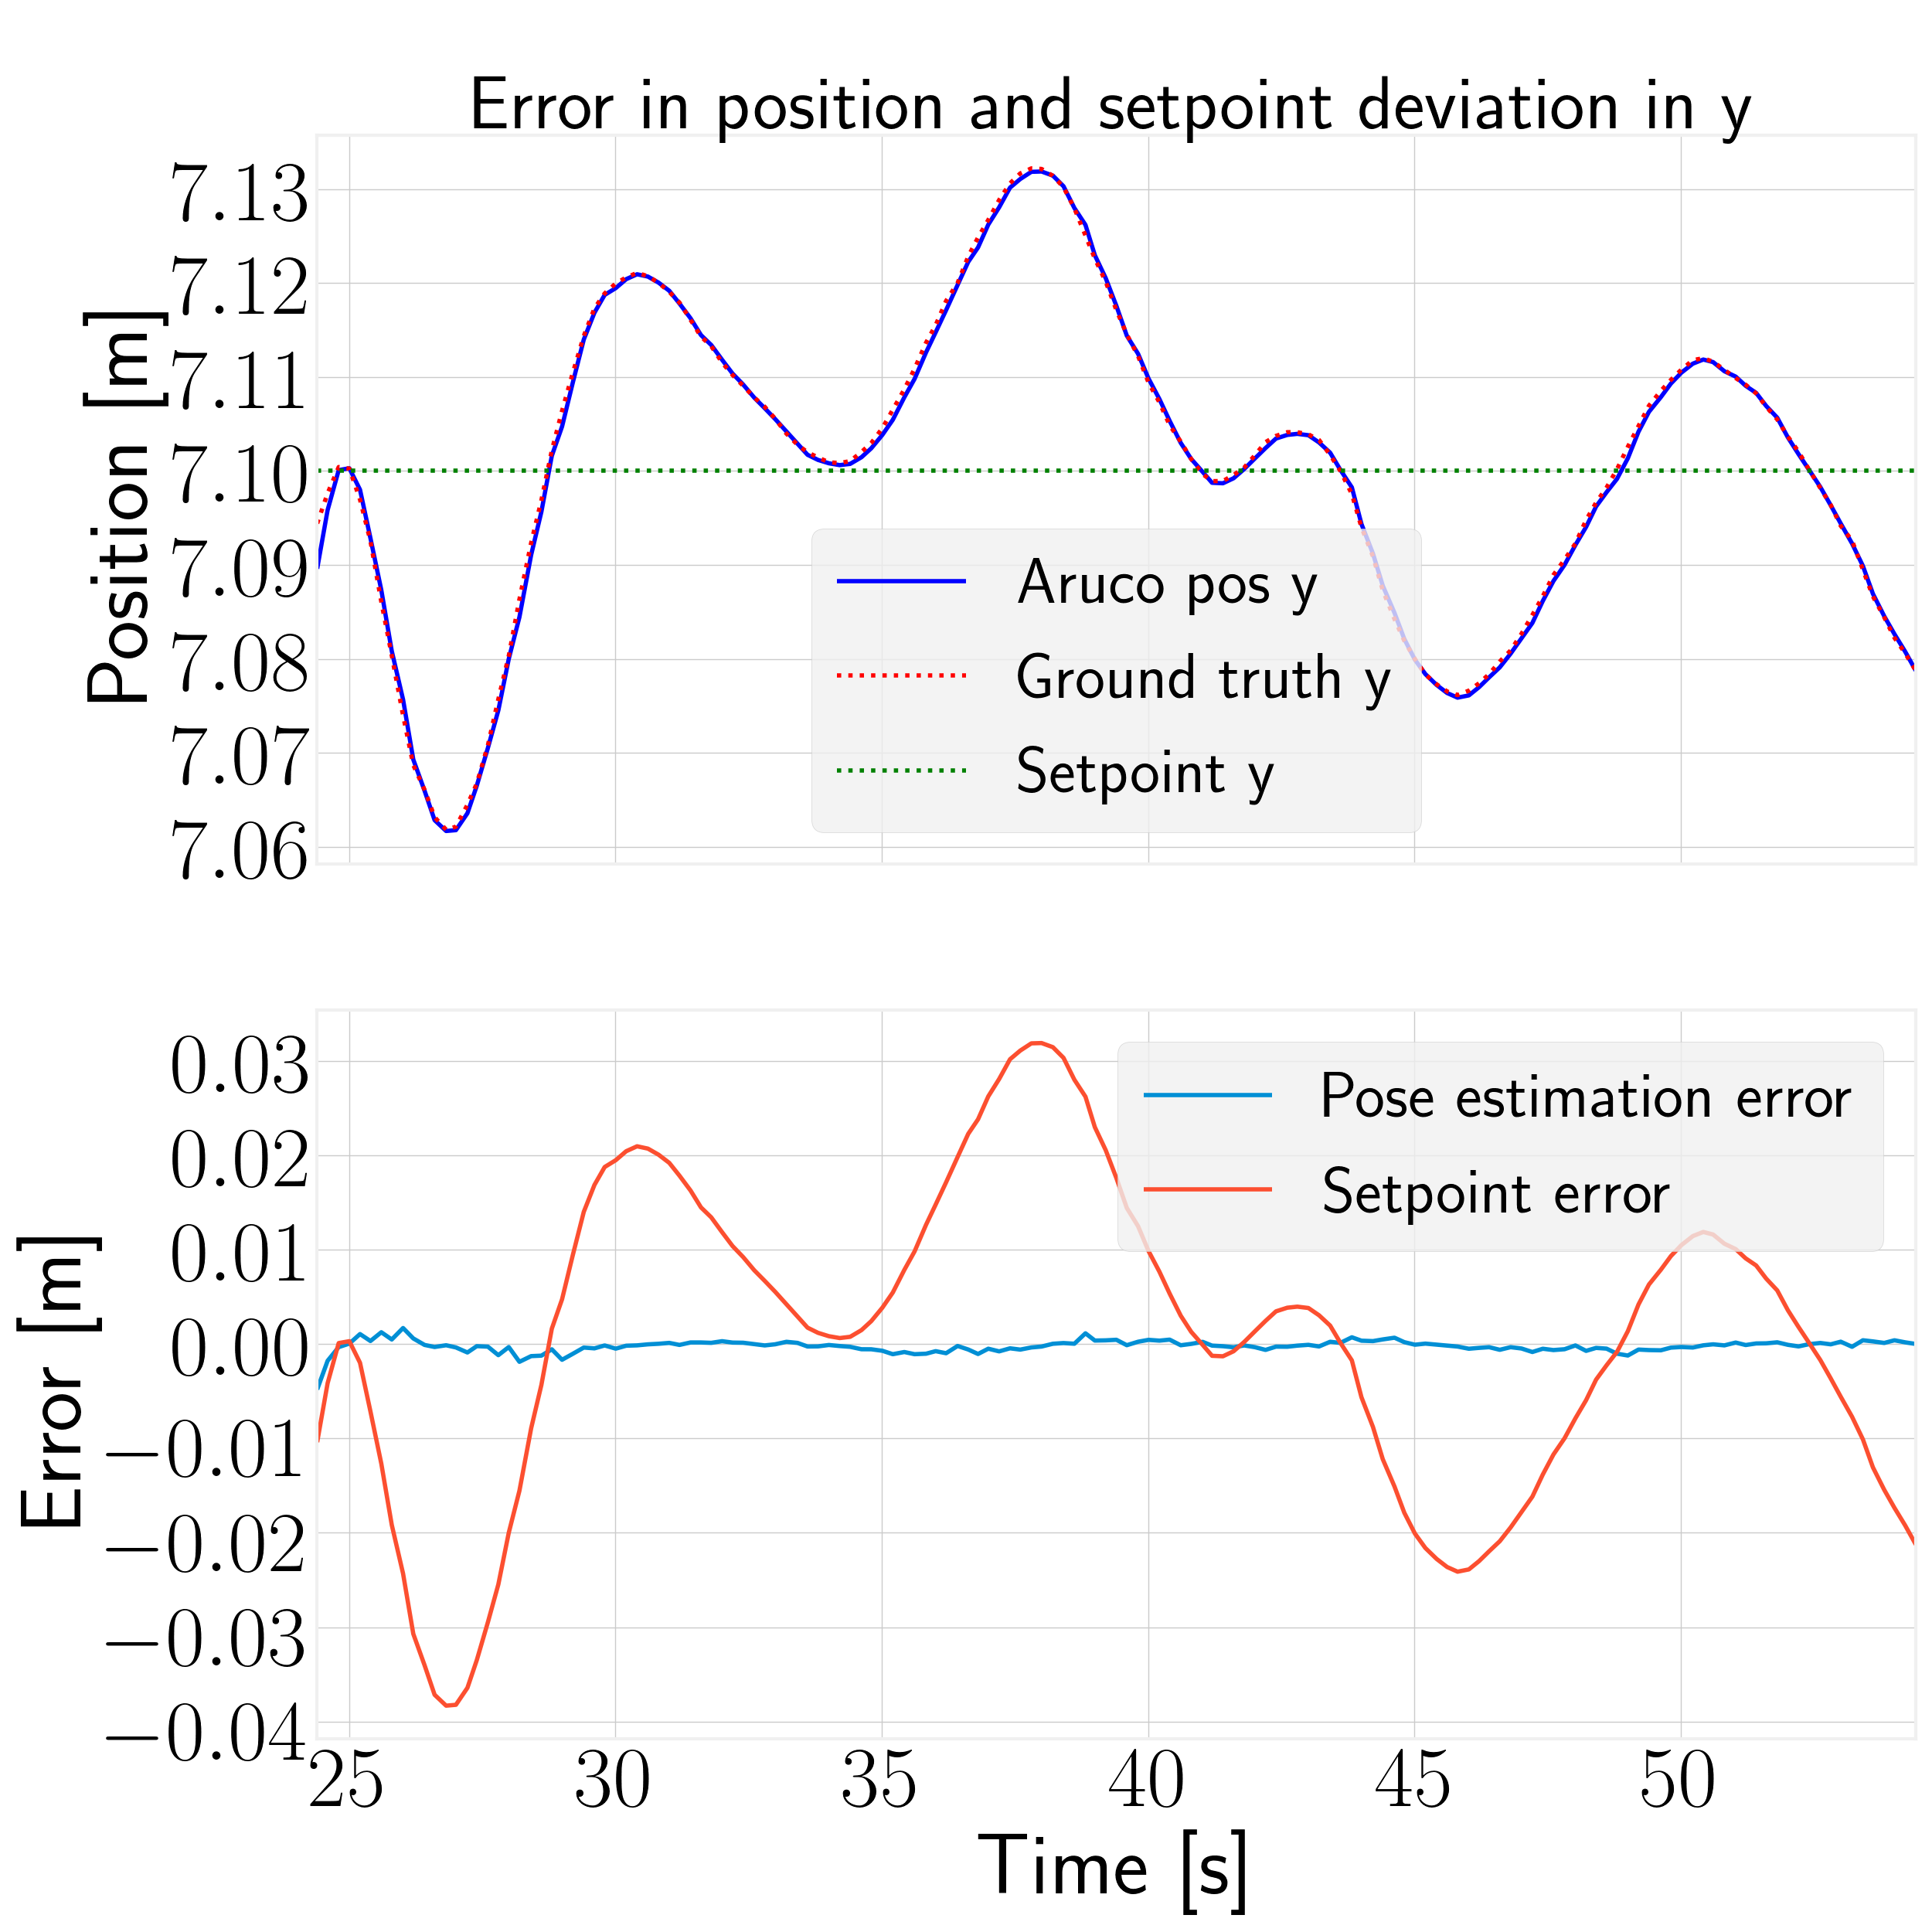
\includegraphics[width=\textwidth]{../Figures//hold_pose_using_aruco_pose_estimation/test5_landingBoard3_noWind/error_y/pose_error_y_test1.png}
        \caption{}
        \label{fig:hold_pose_estimation_test5_y}
    \end{subfigure}
     \hspace{0.2em}
    \begin{subfigure}[t]{.30\textwidth}
        \centering
        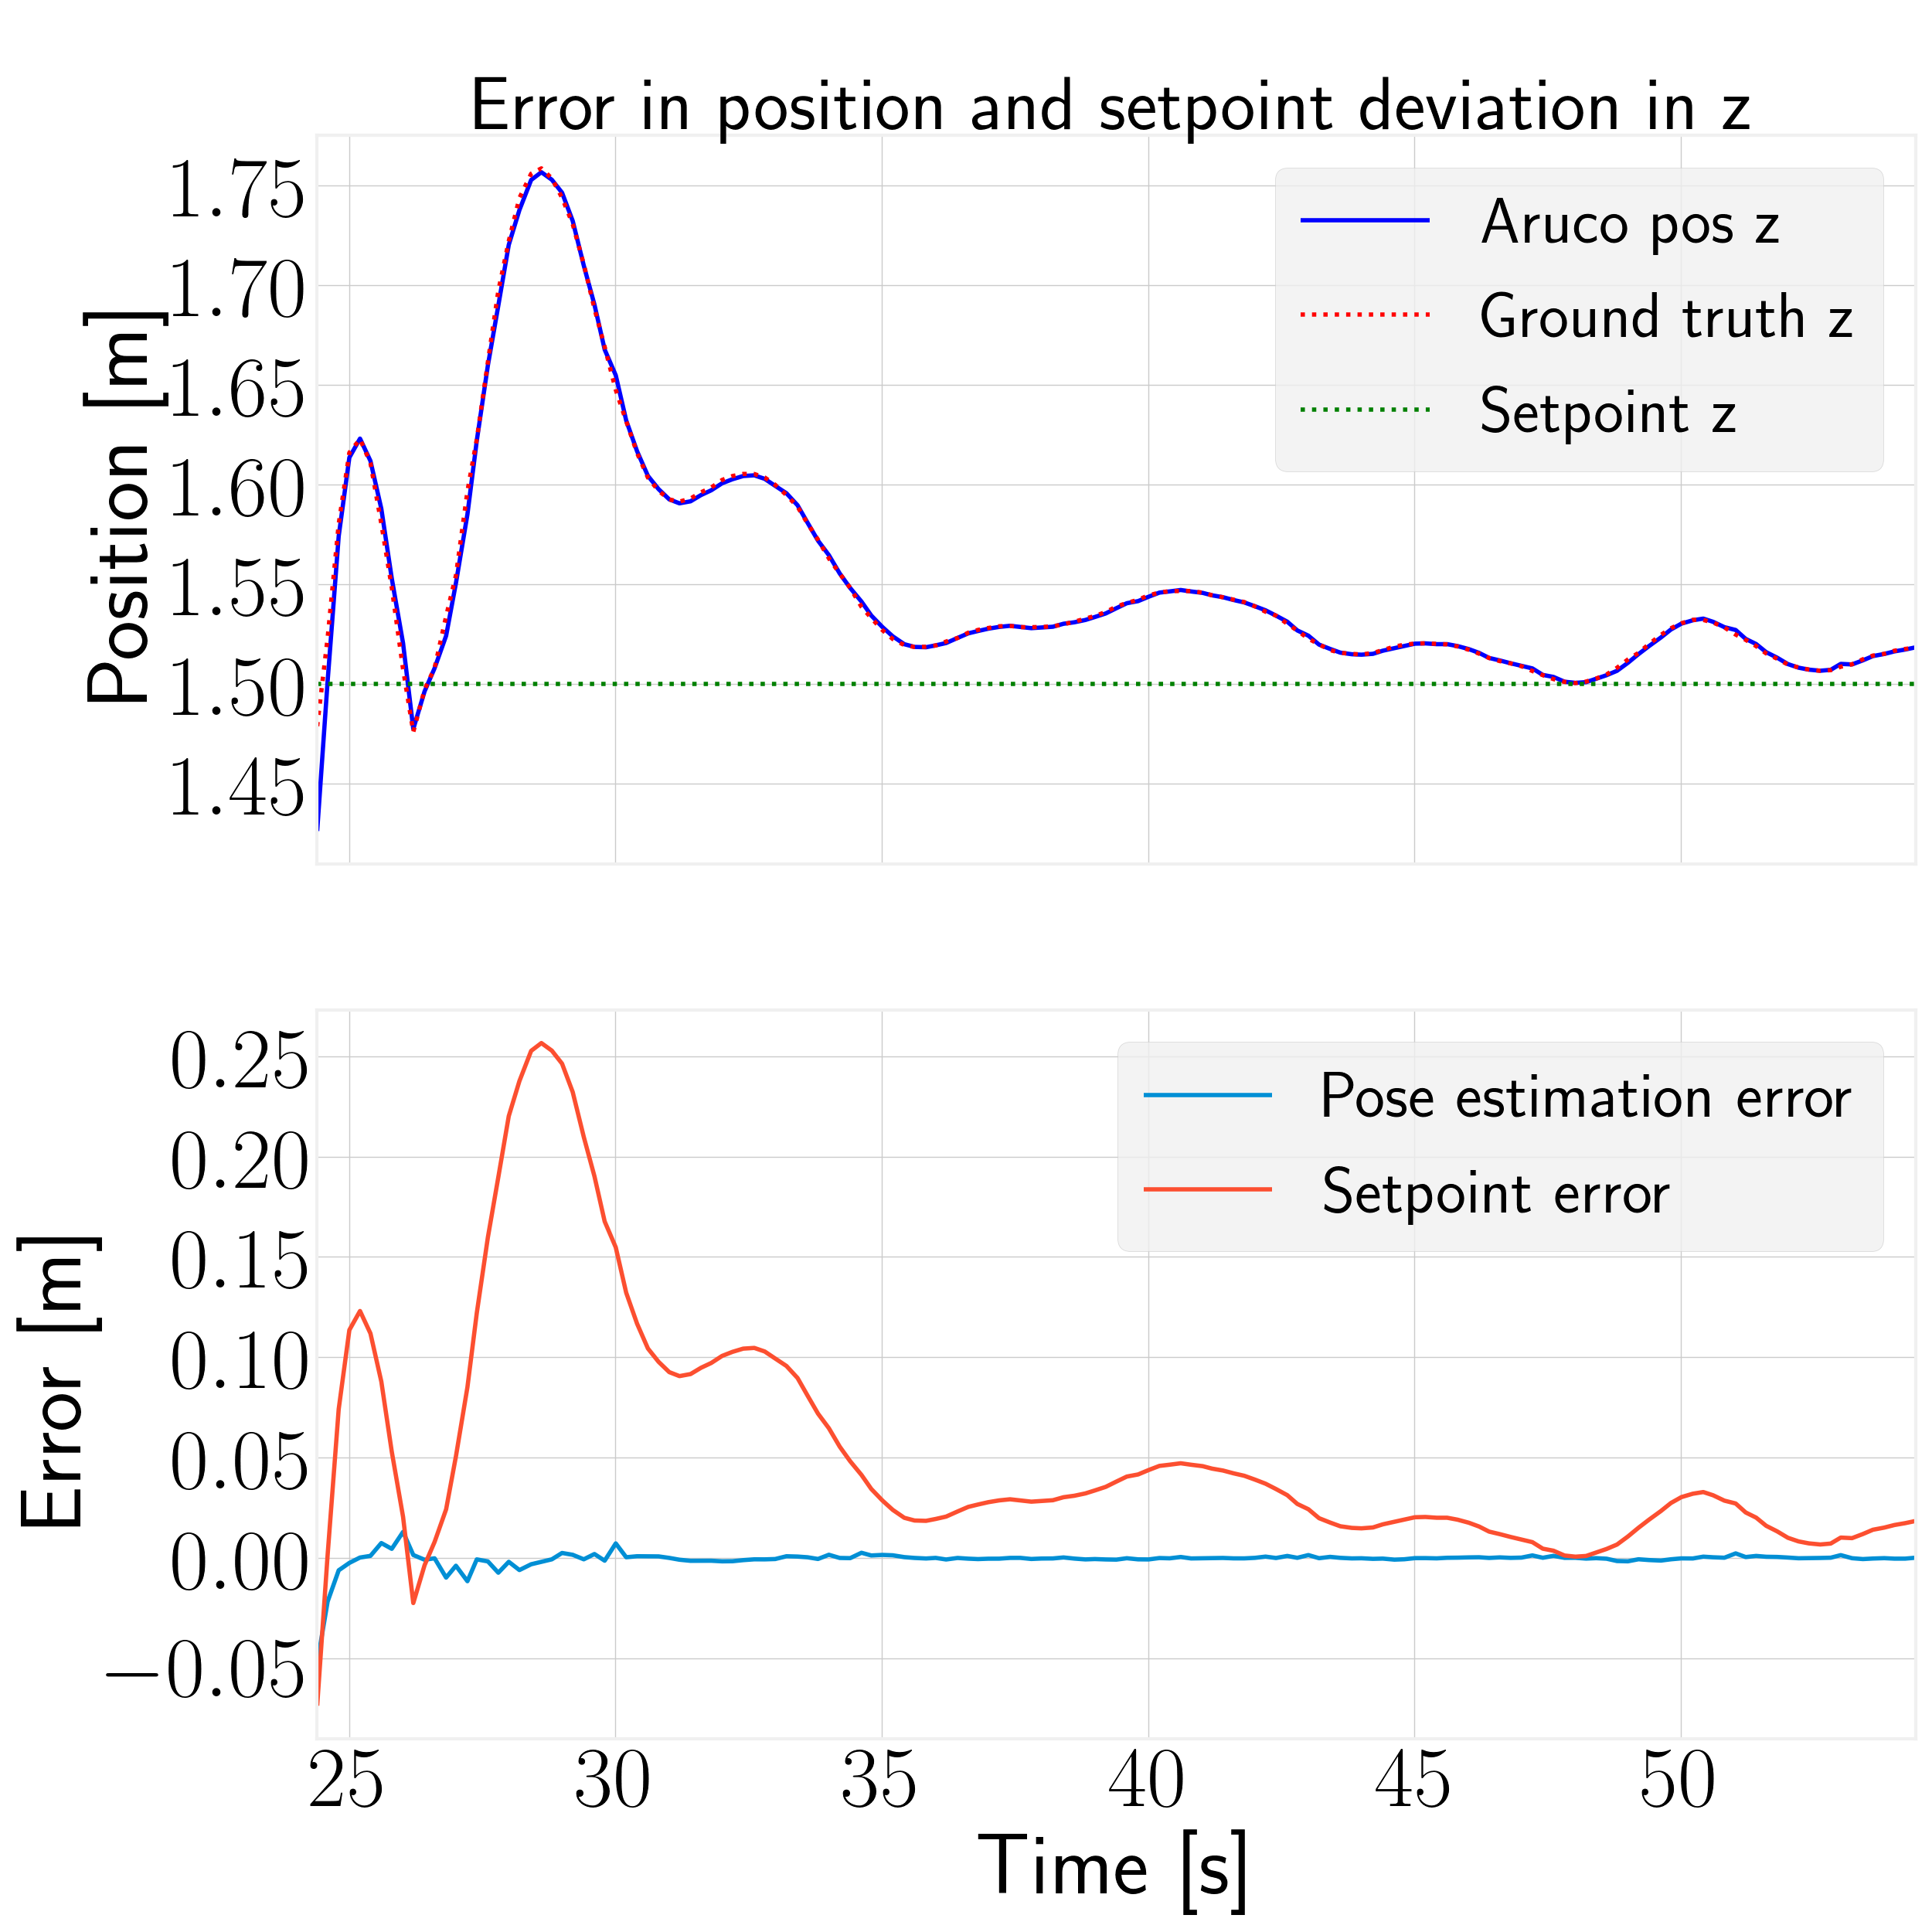
\includegraphics[width=\textwidth]{../Figures/hold_pose_using_aruco_pose_estimation/test5_landingBoard3_noWind/error_z/pose_error_z_test1.png}
        \caption{}
        \label{fig:hold_pose_estimation_test5_z}
    \end{subfigure}
    \caption{}
    \label{fig:hold_pose_estimation_test5_error_pos}
\end{figure}

\begin{figure}[H]
    \centering
    \begin{subfigure}[t]{.30\textwidth}
        \centering
        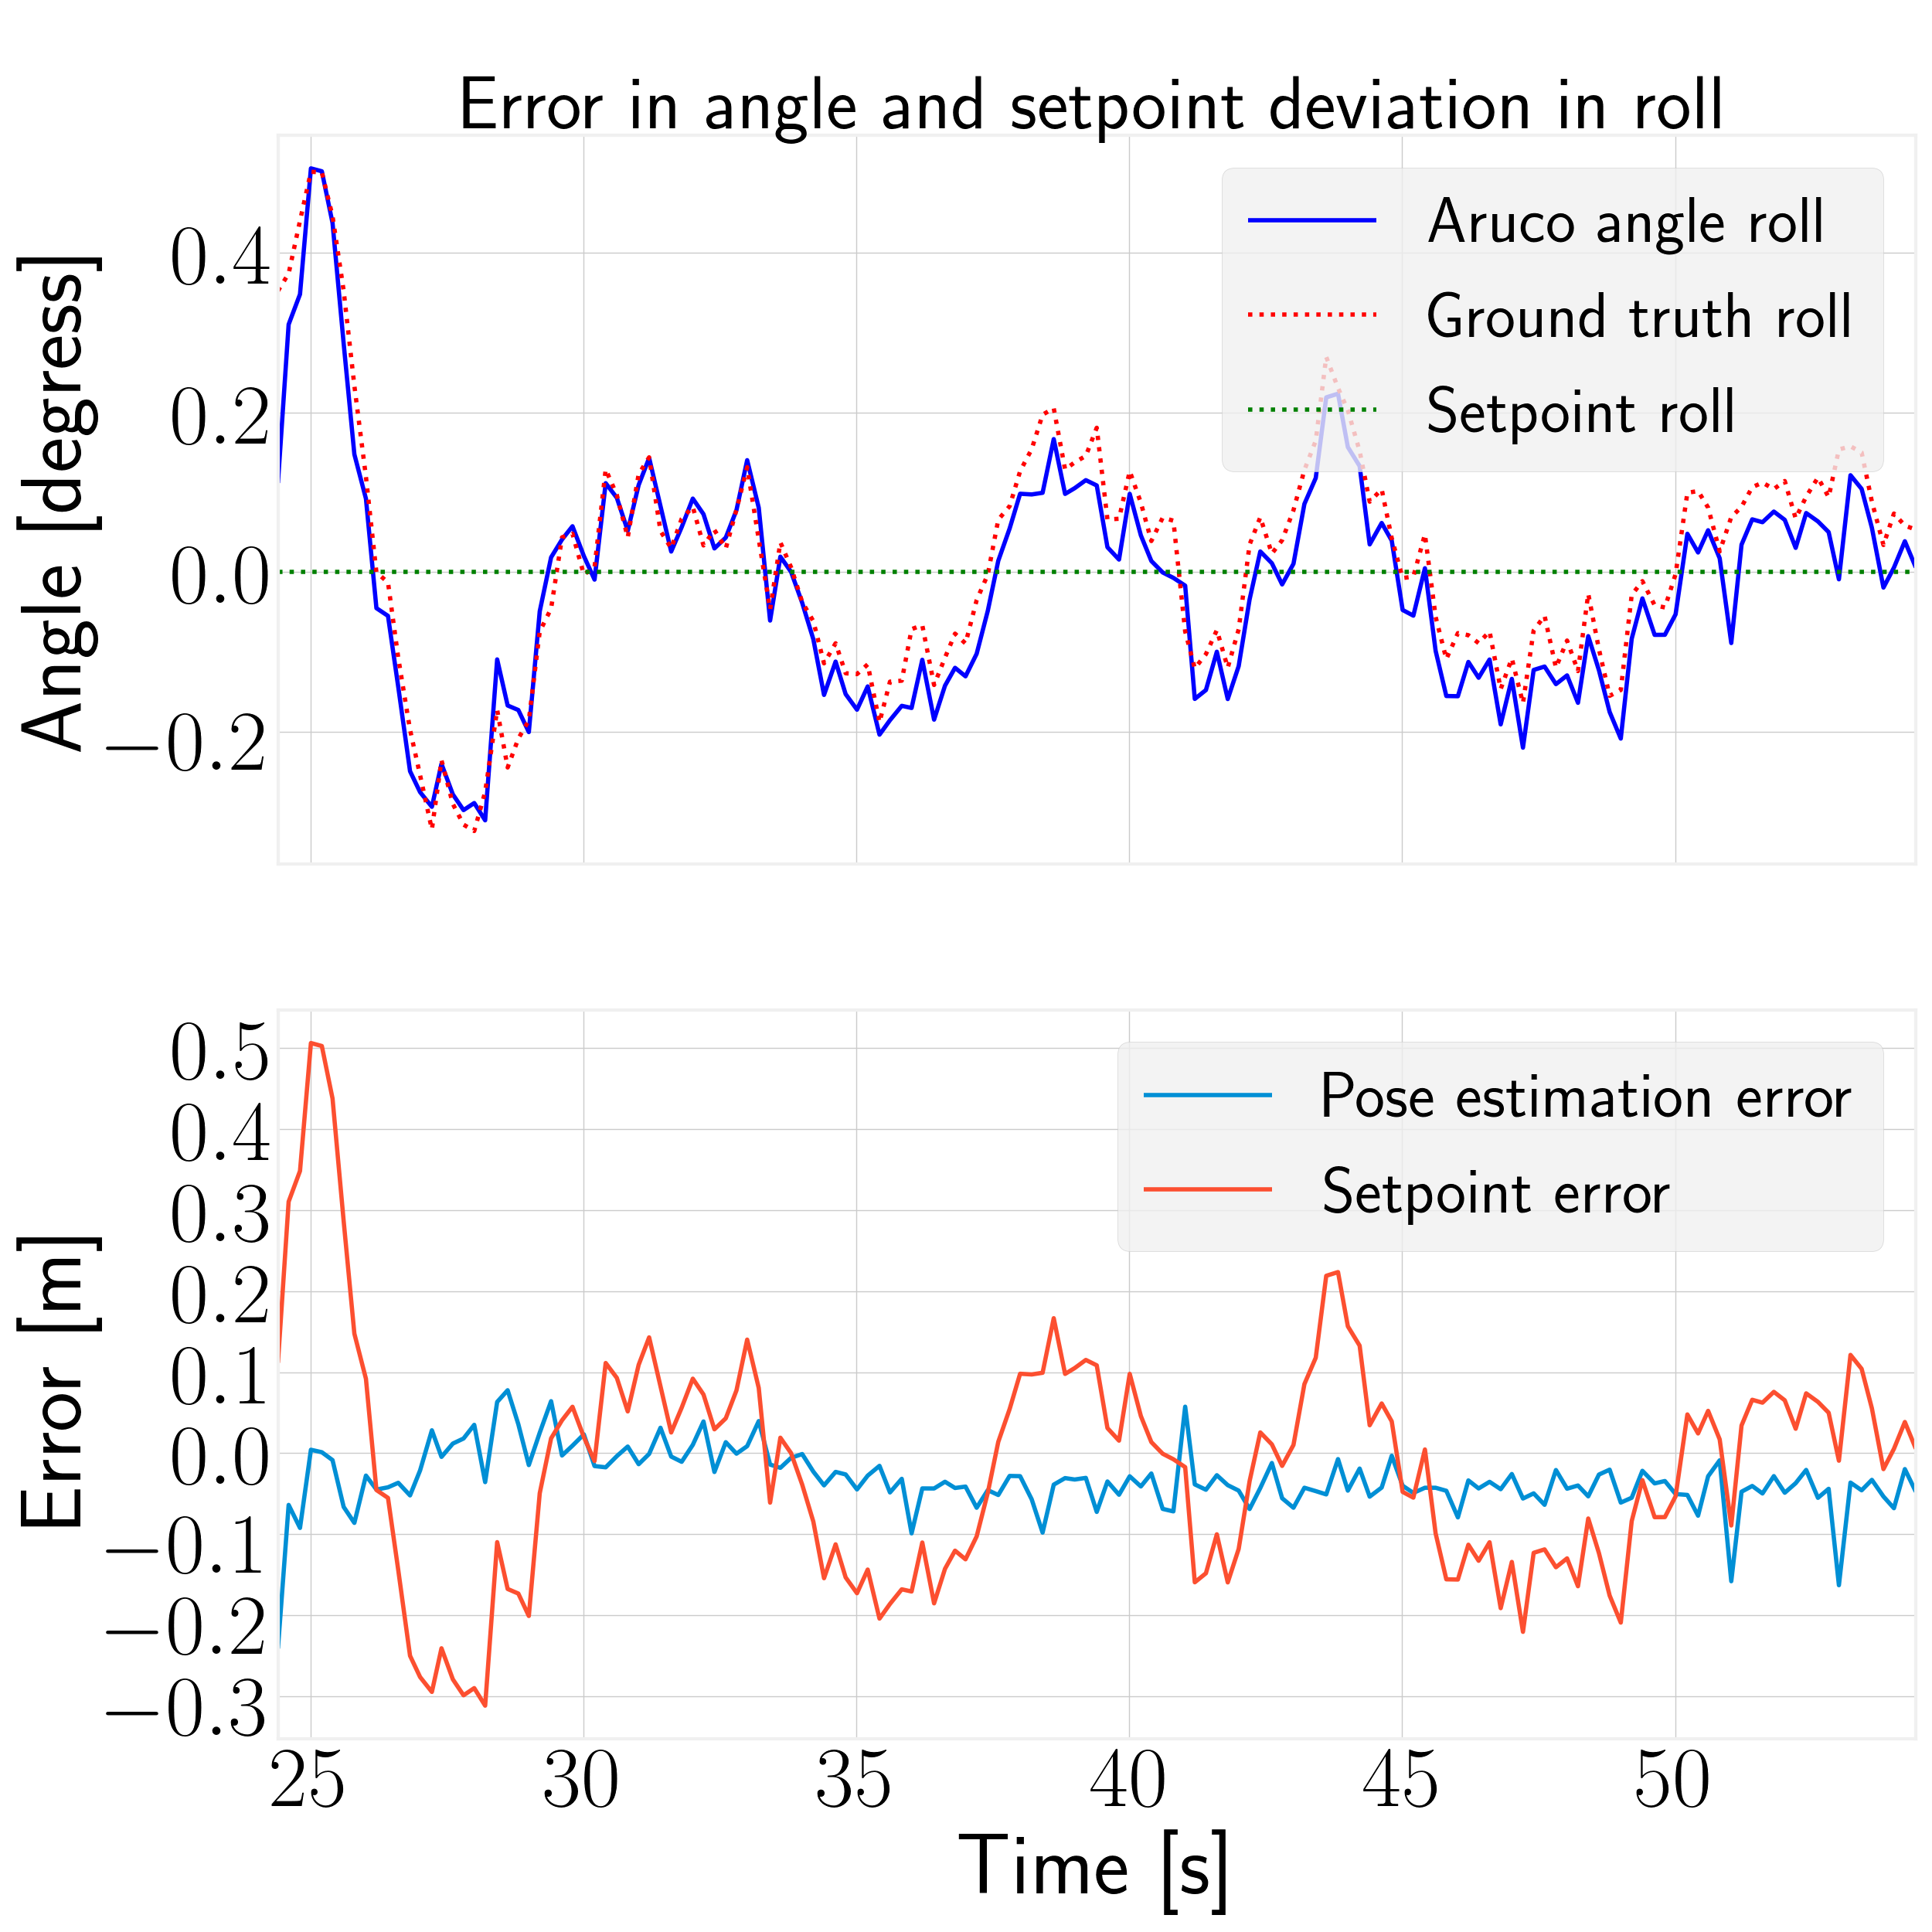
\includegraphics[width=\textwidth]{../Figures/hold_pose_using_aruco_pose_estimation/test5_landingBoard3_noWind/error_roll/pose_error_roll_test1.png}
        \caption{}
        \label{fig:hold_pose_estimation_test5_roll}
    \end{subfigure}
     \hspace{0.2em}
    \begin{subfigure}[t]{.30\textwidth}
        \centering
        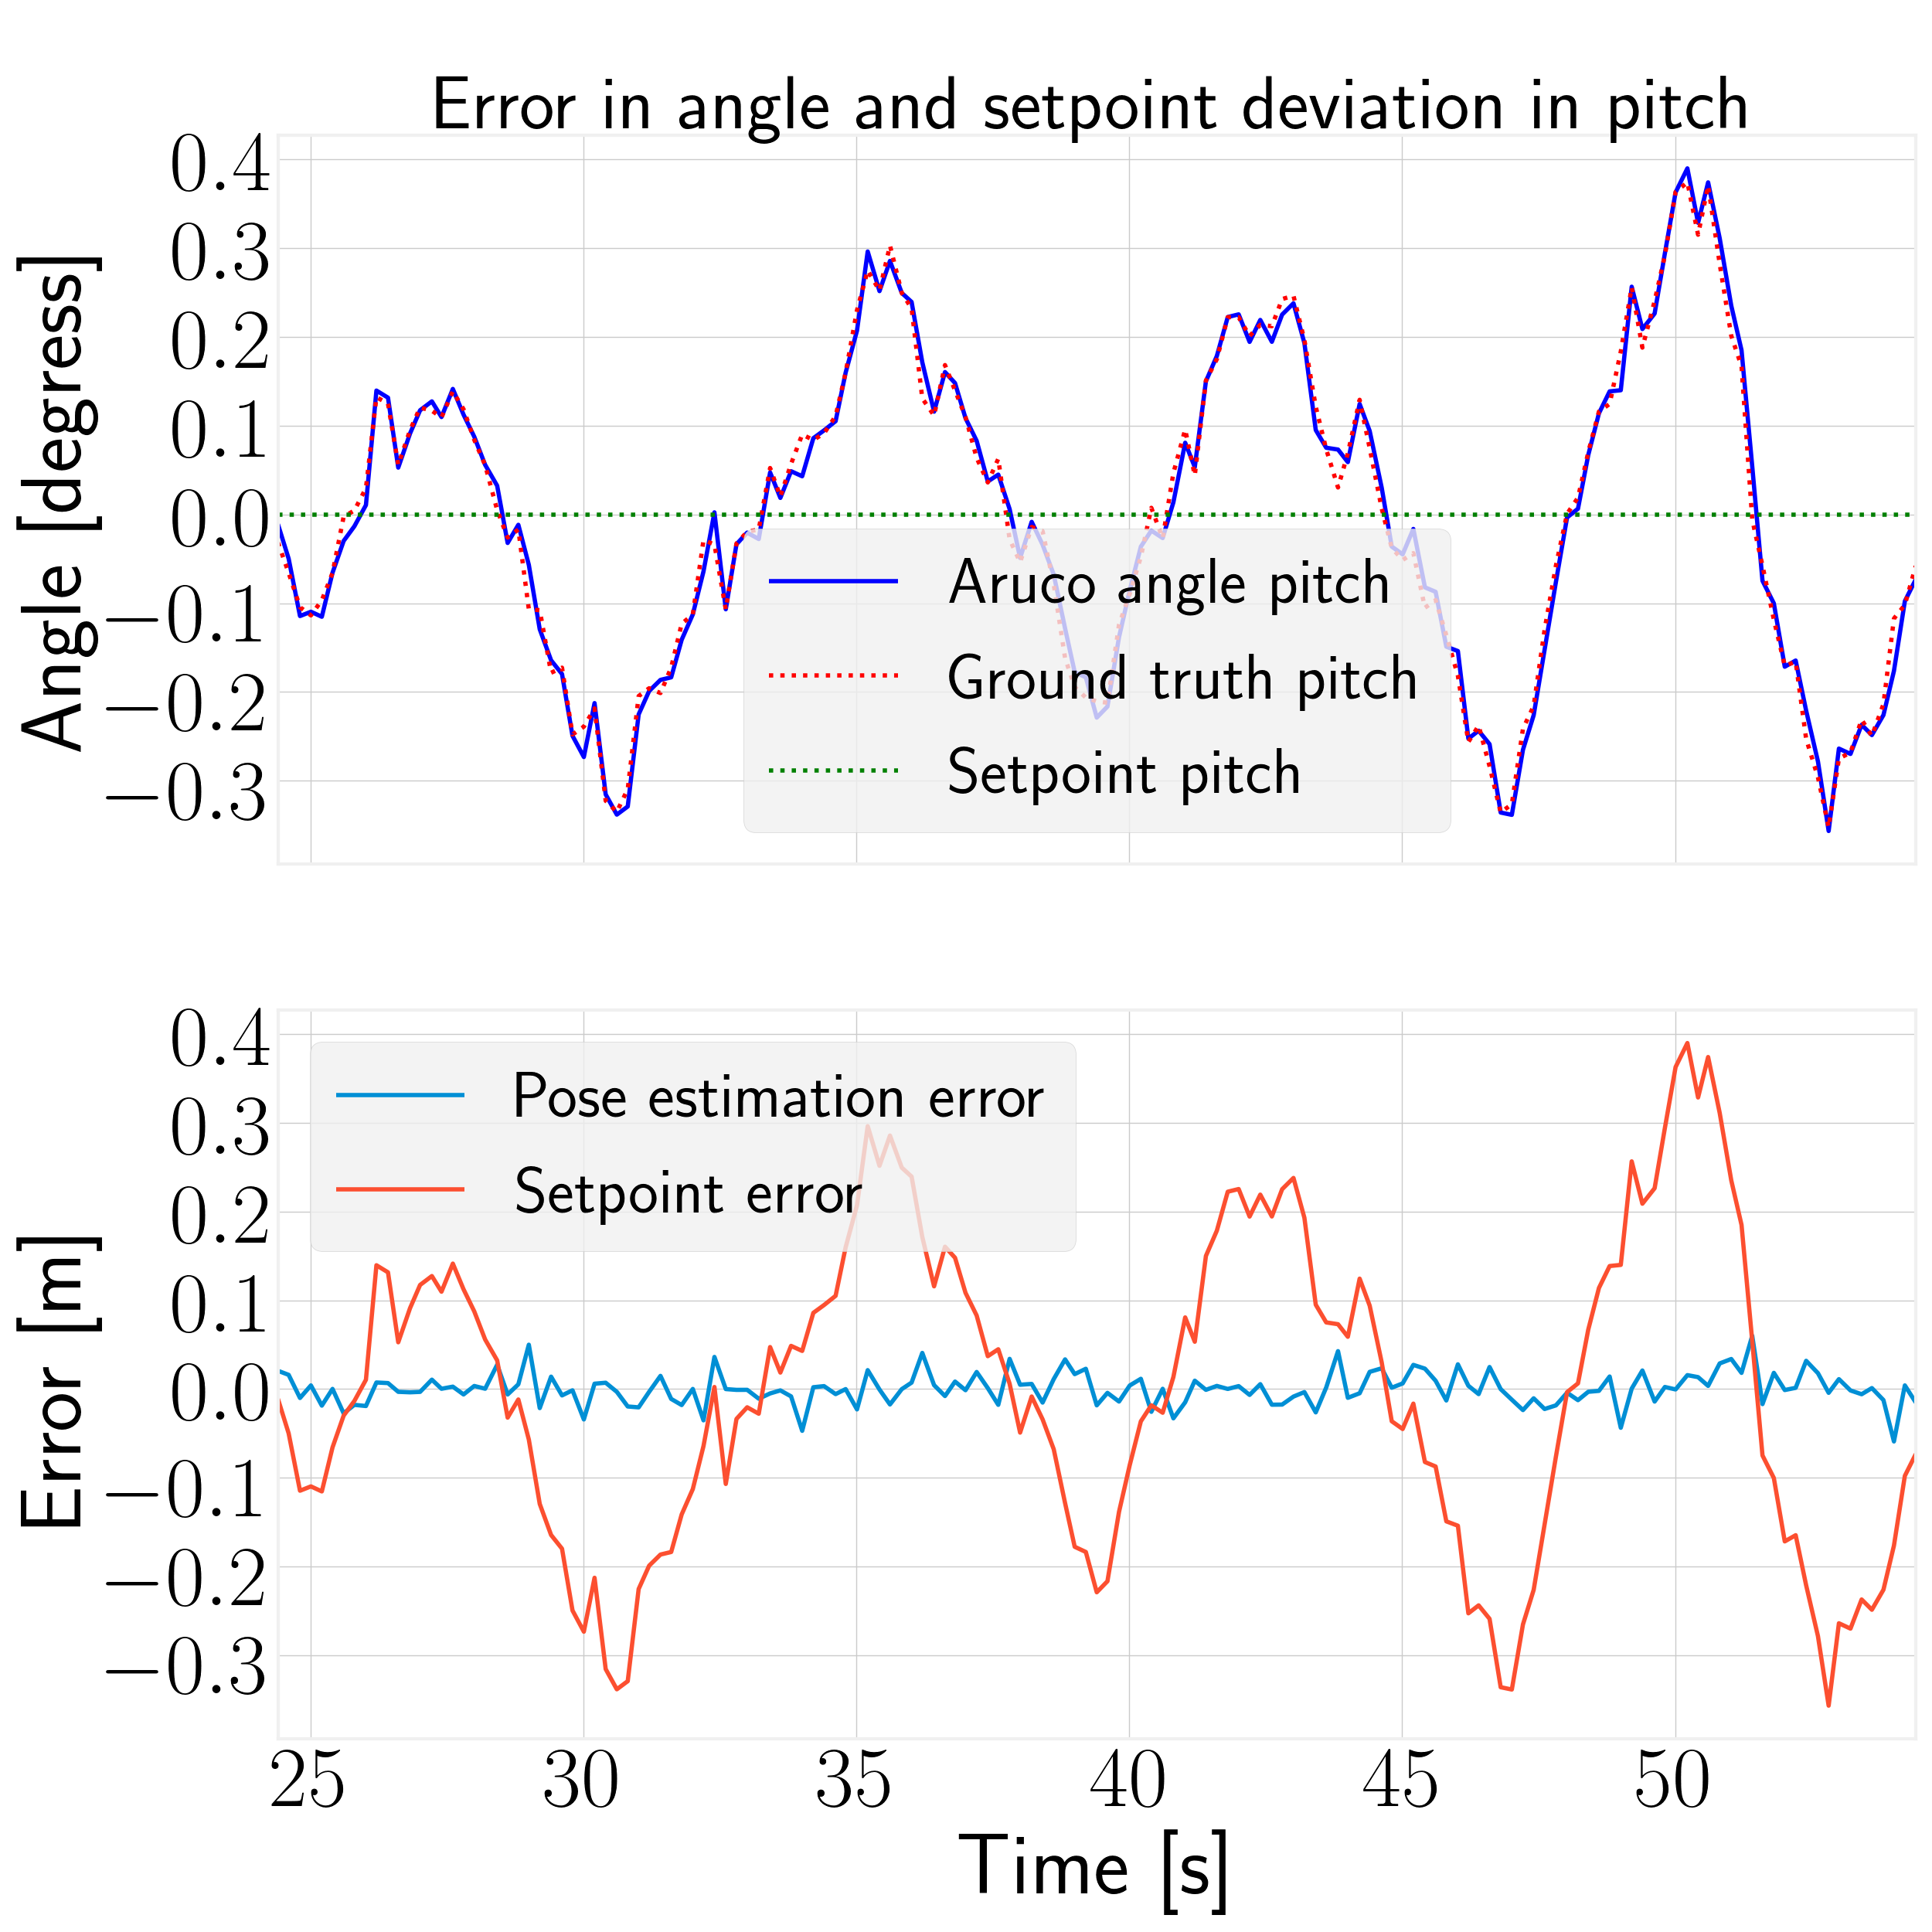
\includegraphics[width=\textwidth]{../Figures//hold_pose_using_aruco_pose_estimation/test5_landingBoard3_noWind/error_pitch/pose_error_pitch_test1.png}
        \caption{}
        \label{fig:hold_pose_estimation_test5_pitch}
    \end{subfigure}
     \hspace{0.2em}
    \begin{subfigure}[t]{.30\textwidth}
        \centering
        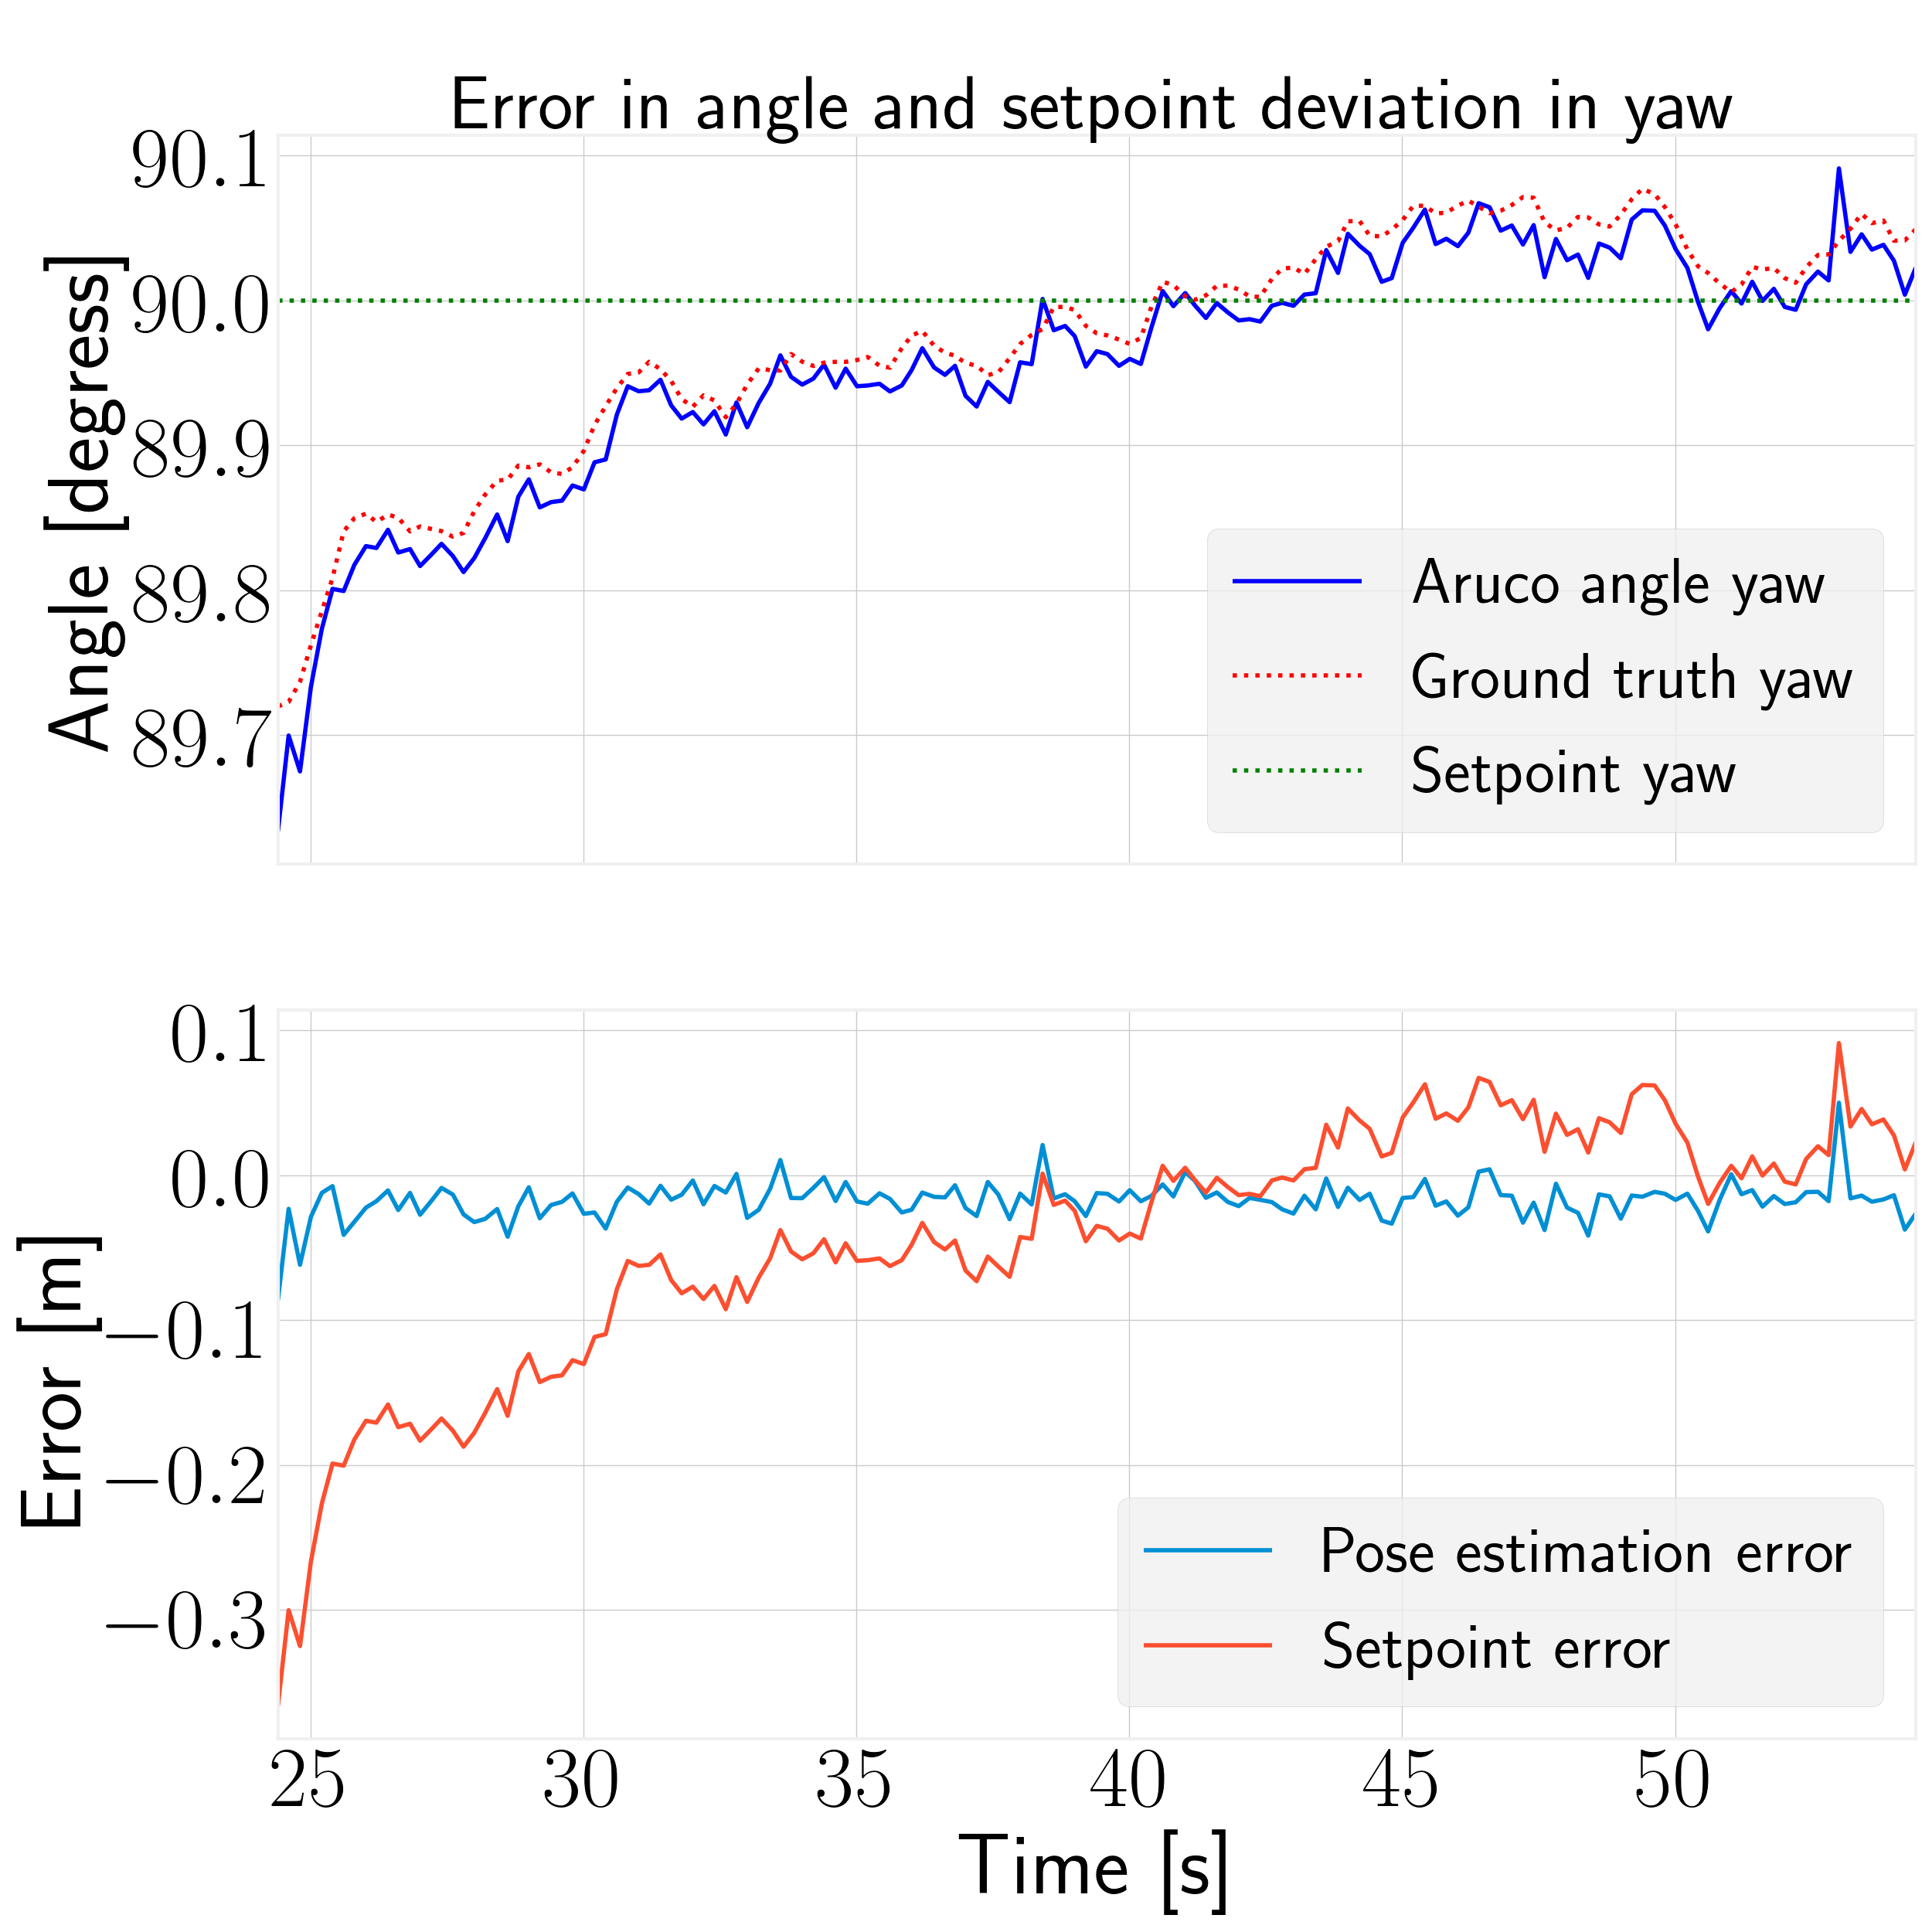
\includegraphics[width=\textwidth]{../Figures/hold_pose_using_aruco_pose_estimation/test5_landingBoard3_noWind/error_yaw/pose_error_yaw_test1.png}
        \caption{}
        \label{fig:hold_pose_estimation_test5_yaw}
    \end{subfigure}
    \caption{}
    \label{fig:hold_pose_estimation_test5_error_angle}
\end{figure}

\subsubsection{GPS to vision navigation}
\label{sec:gps2vision_transition}

\begin{figure}[H]
    \centering
    \begin{subfigure}[t]{.30\textwidth}
        \centering
        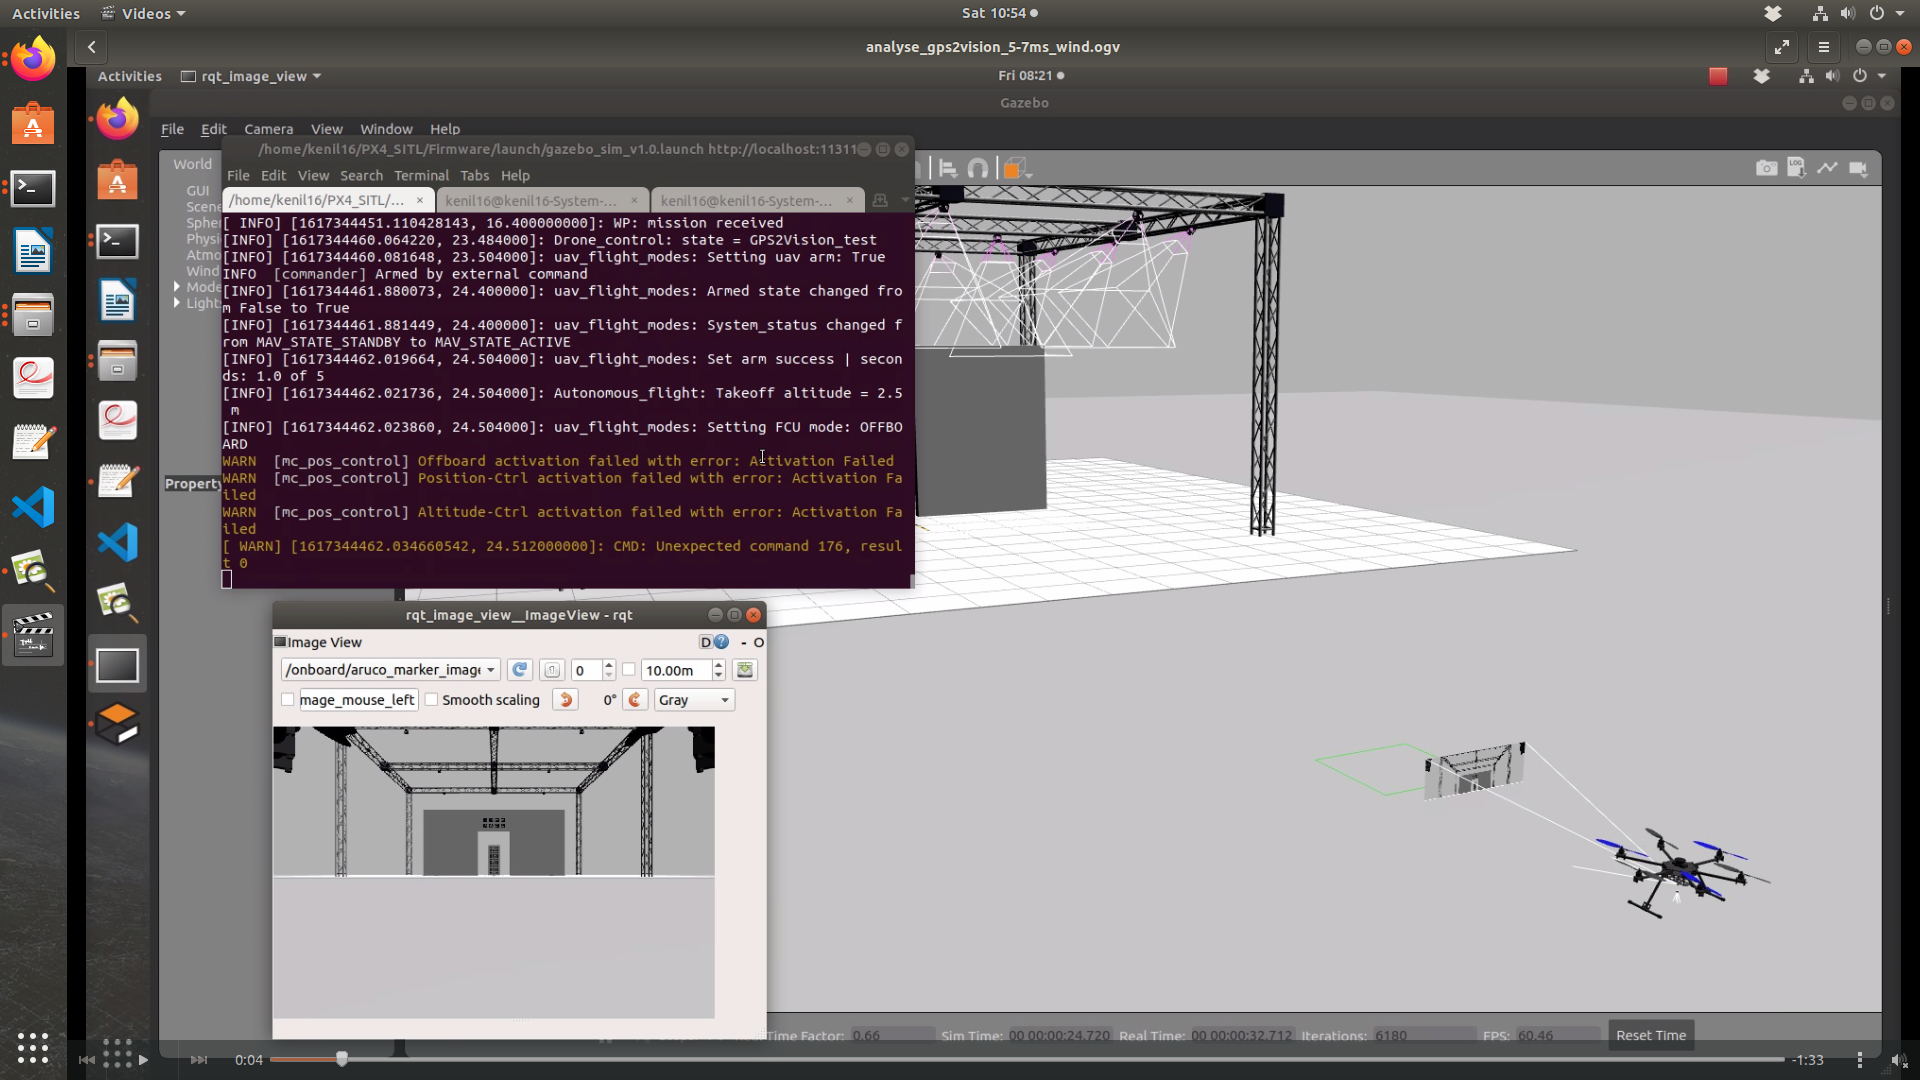
\includegraphics[width=\textwidth]{../Figures/GPS2Vision/drone_start_pose_gps.png}
        \caption{}
        \label{fig:gps2vision_gps}
    \end{subfigure}
     \hspace{0.2em}
    \begin{subfigure}[t]{.30\textwidth}
        \centering
        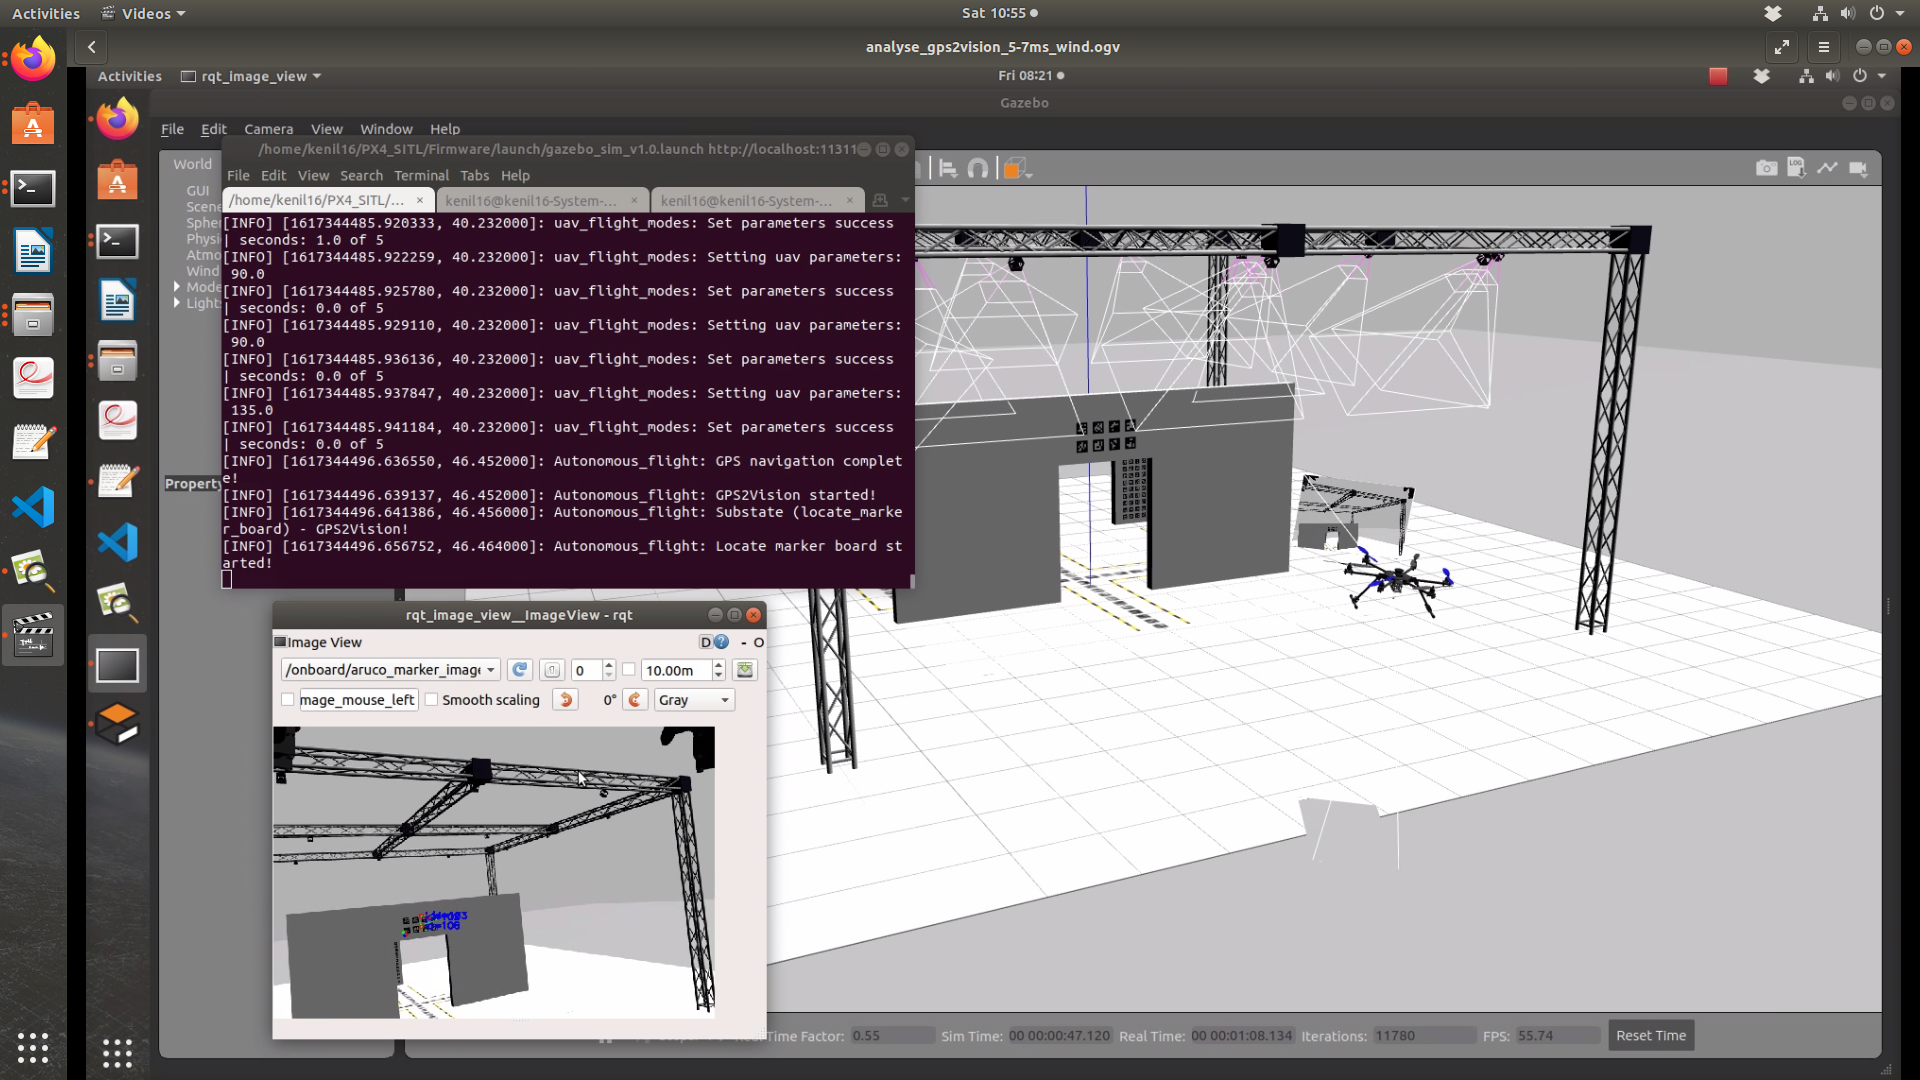
\includegraphics[width=\textwidth]{../Figures/GPS2Vision/drone_locate_board.png}
        \caption{}
        \label{fig:gps2vision_locate_board}
    \end{subfigure}
         \hspace{0.2em}
    \begin{subfigure}[t]{.30\textwidth}
        \centering
        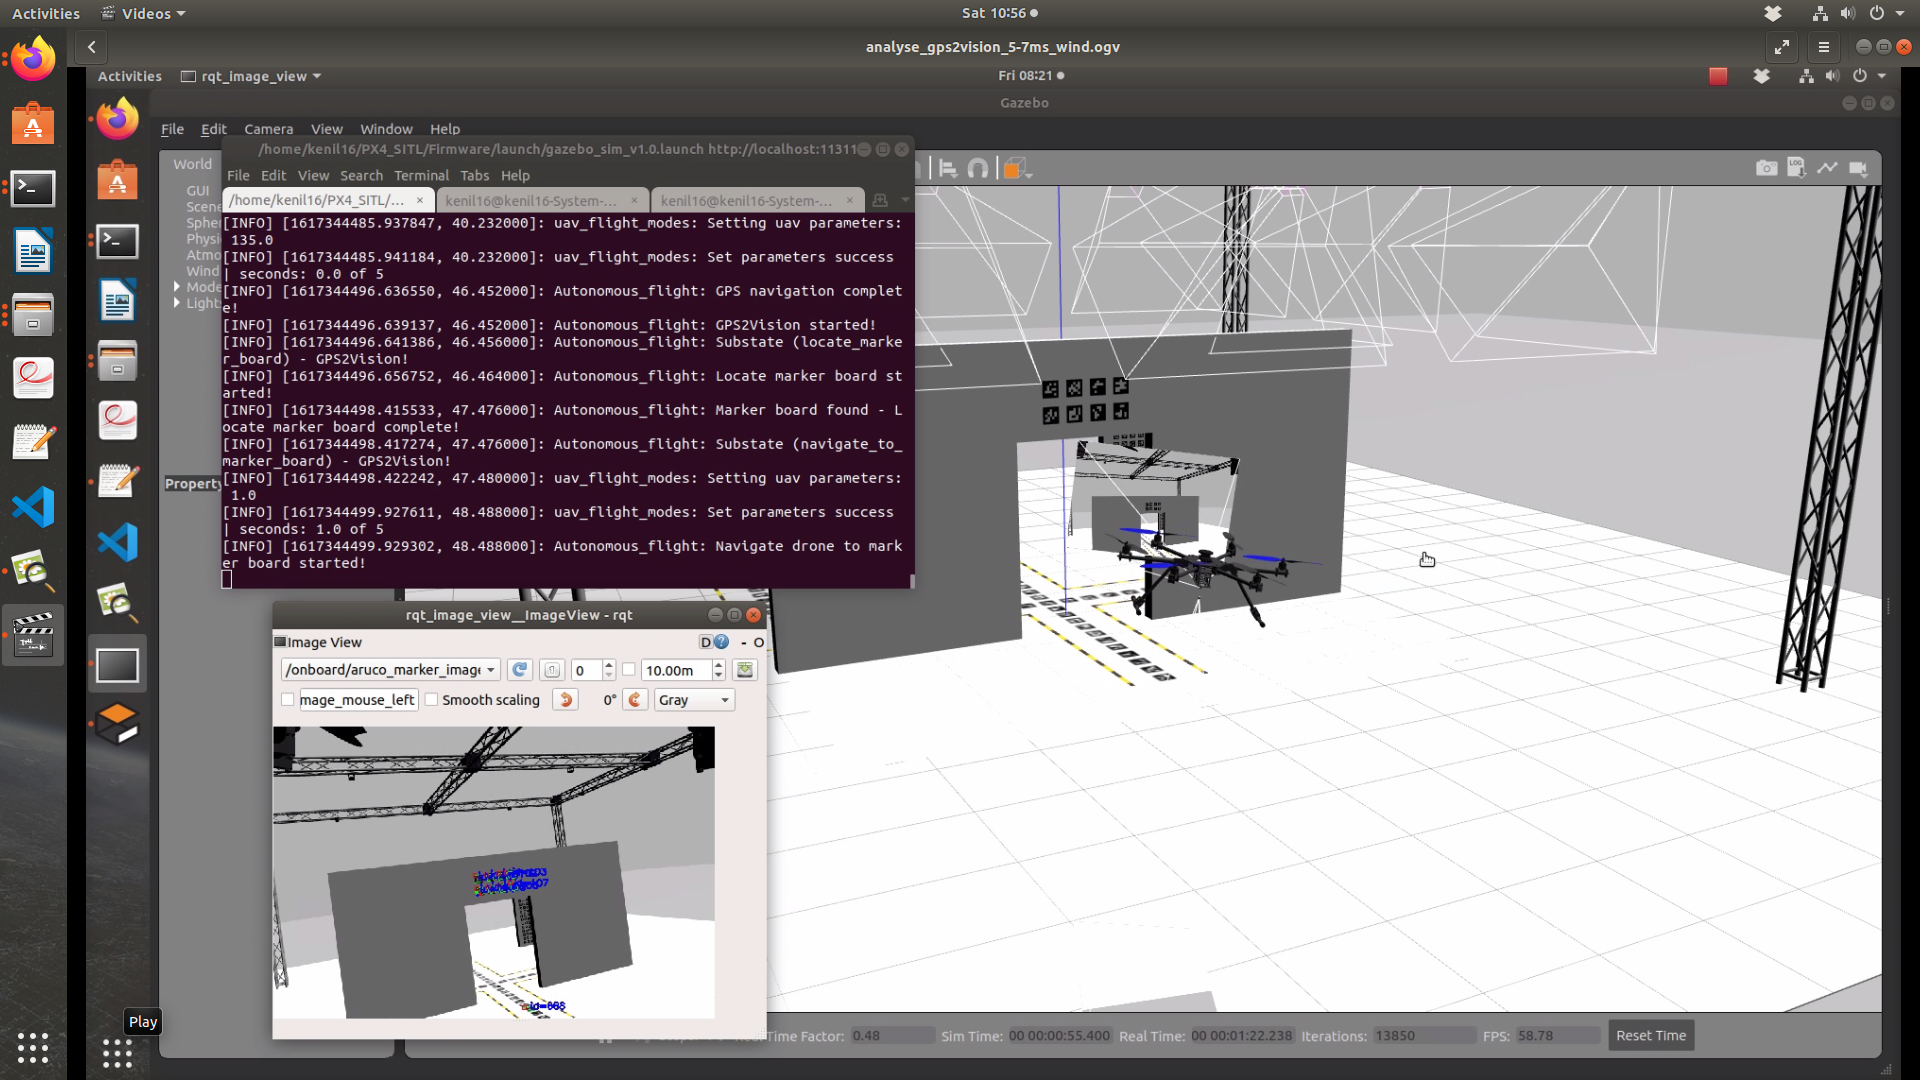
\includegraphics[width=\textwidth]{../Figures/GPS2Vision/drone_navigate_to_board.png}
        \caption{}
        \label{fig:gps2vision_navigate_to_board}
    \end{subfigure}
         \hspace{0.2em}
    \begin{subfigure}[t]{.30\textwidth}
        \centering
        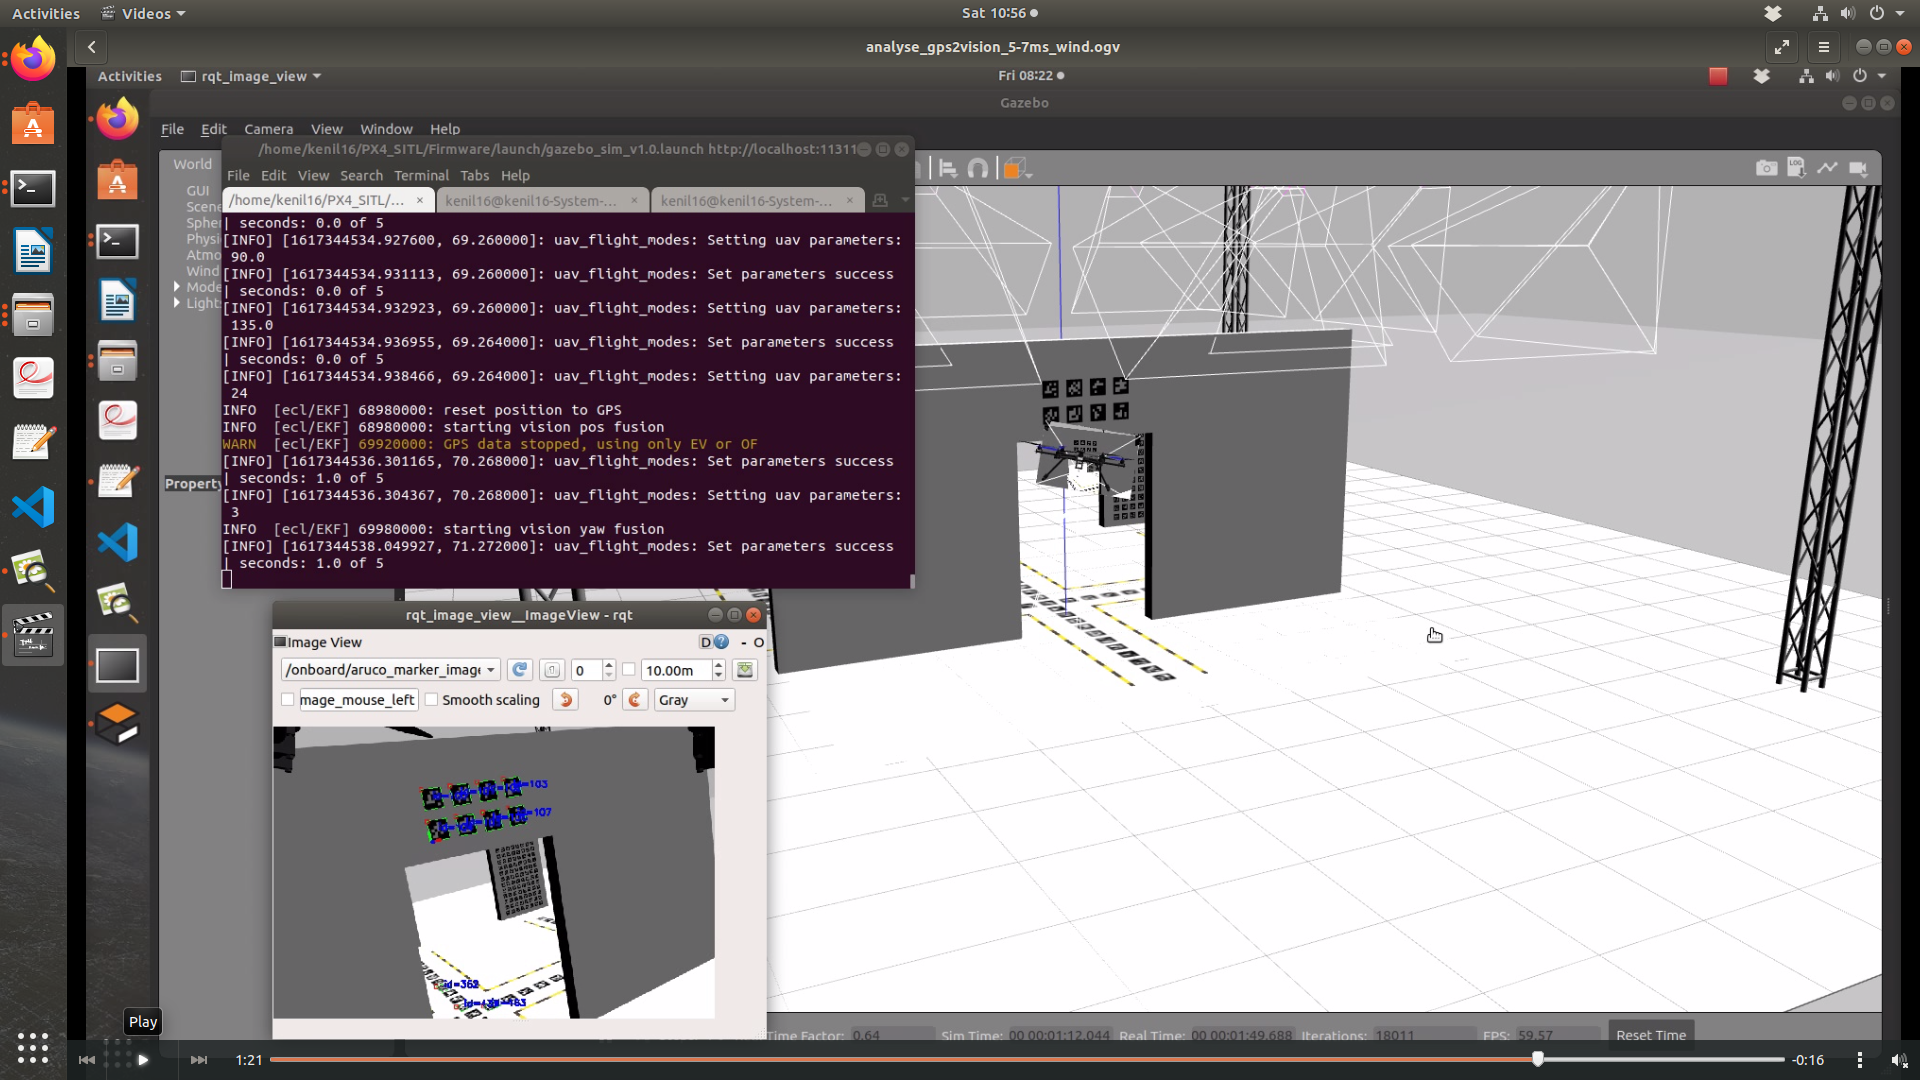
\includegraphics[width=\textwidth]{../Figures/GPS2Vision/drone_gps2vision_transition.png}
        \caption{}
        \label{fig:gps2vision_gps2vision_transition}
    \end{subfigure}
         \hspace{0.2em}
    \begin{subfigure}[t]{.30\textwidth}
        \centering
        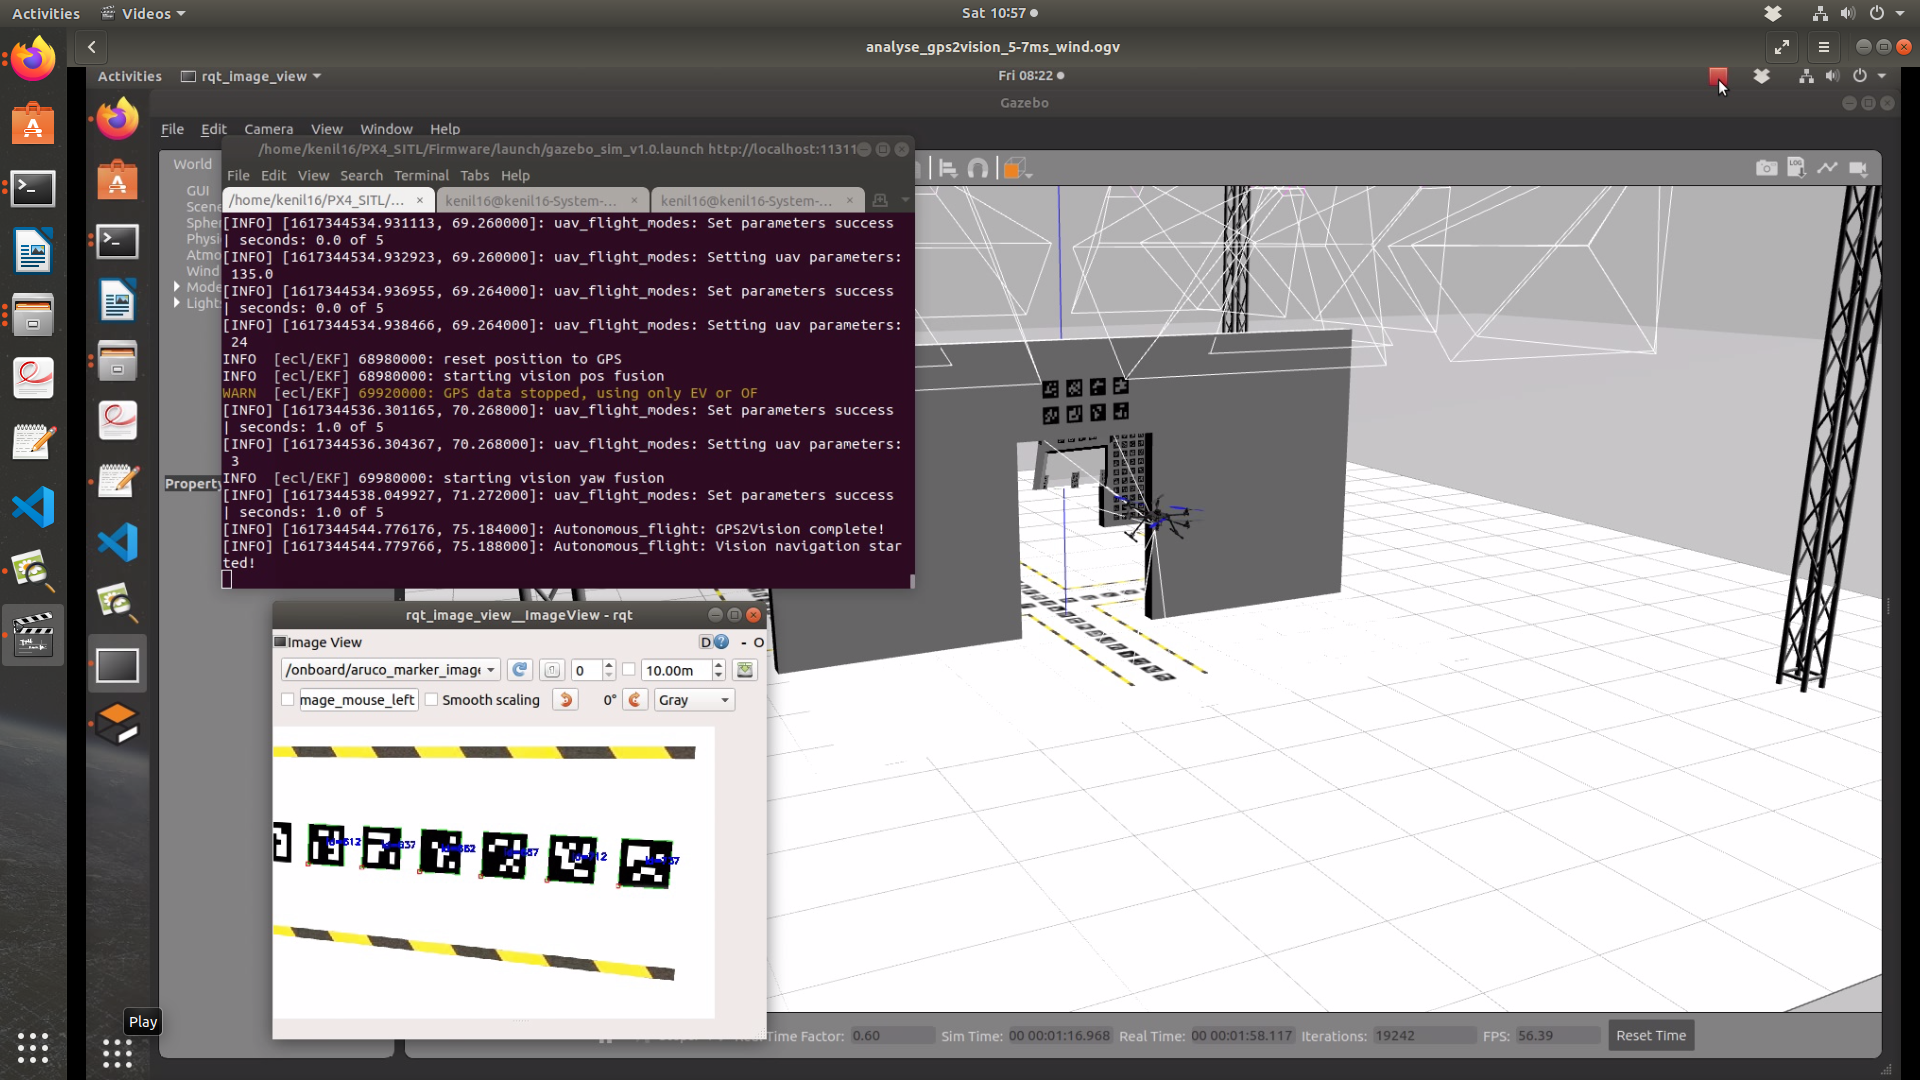
\includegraphics[width=\textwidth]{../Figures/GPS2Vision/drone_vision_navigation.png}
        \caption{}
        \label{fig:gps2vision_vision_navigation}
    \end{subfigure}
    \caption{}
    \label{fig:gps2vision_states}
\end{figure}

\begin{table}[H]
    \centering
    \addtolength{\leftskip} {-2cm}
    \addtolength{\rightskip}{-2cm}
        \caption{Statistics of the results from landing tests }
        \pgfplotstabletypeset[normal,
                columns/eg/.style={
                column name={Runs},
                dec sep align
        }
        ]{ %
       Wind & eg & Completed & Vel (GPS) & GPS & Locate board & Navigate to board & Vel (vision) & GPS2Vision\\
        \topmidheader{10}{\textbf{Test 1}}
          0 $\frac{m}{s}$ & 20 & 20 & $2\frac{m}{s}$ & $7.45s$ & $0.50s$ & $14.64s$ & $1\frac{m}{s}$ & $5.28s$\\
          \midheader{10}{\textbf{Test 2}}
               5-7 $\frac{m}{s}$ & 20 & 20 & $2 \frac{m}{s}$ & $6.66s$ & $1.76s$ & $16.05s$ & 1$\frac{m}{s}$ & $5.32s$\\
                  \midheader{10}{\textbf{Test 3}}
               7-10 $\frac{m}{s}$ & 20 & 17 & $2\frac{m}{s}$ & $7.04s$ & $3.71s$ & $16.24s$ & $1\frac{m}{s}$& $20.39s$\\
}
\end{table}


\begin{figure}[H]
    \centering
    \begin{subfigure}[t]{.45\textwidth}
        \centering
        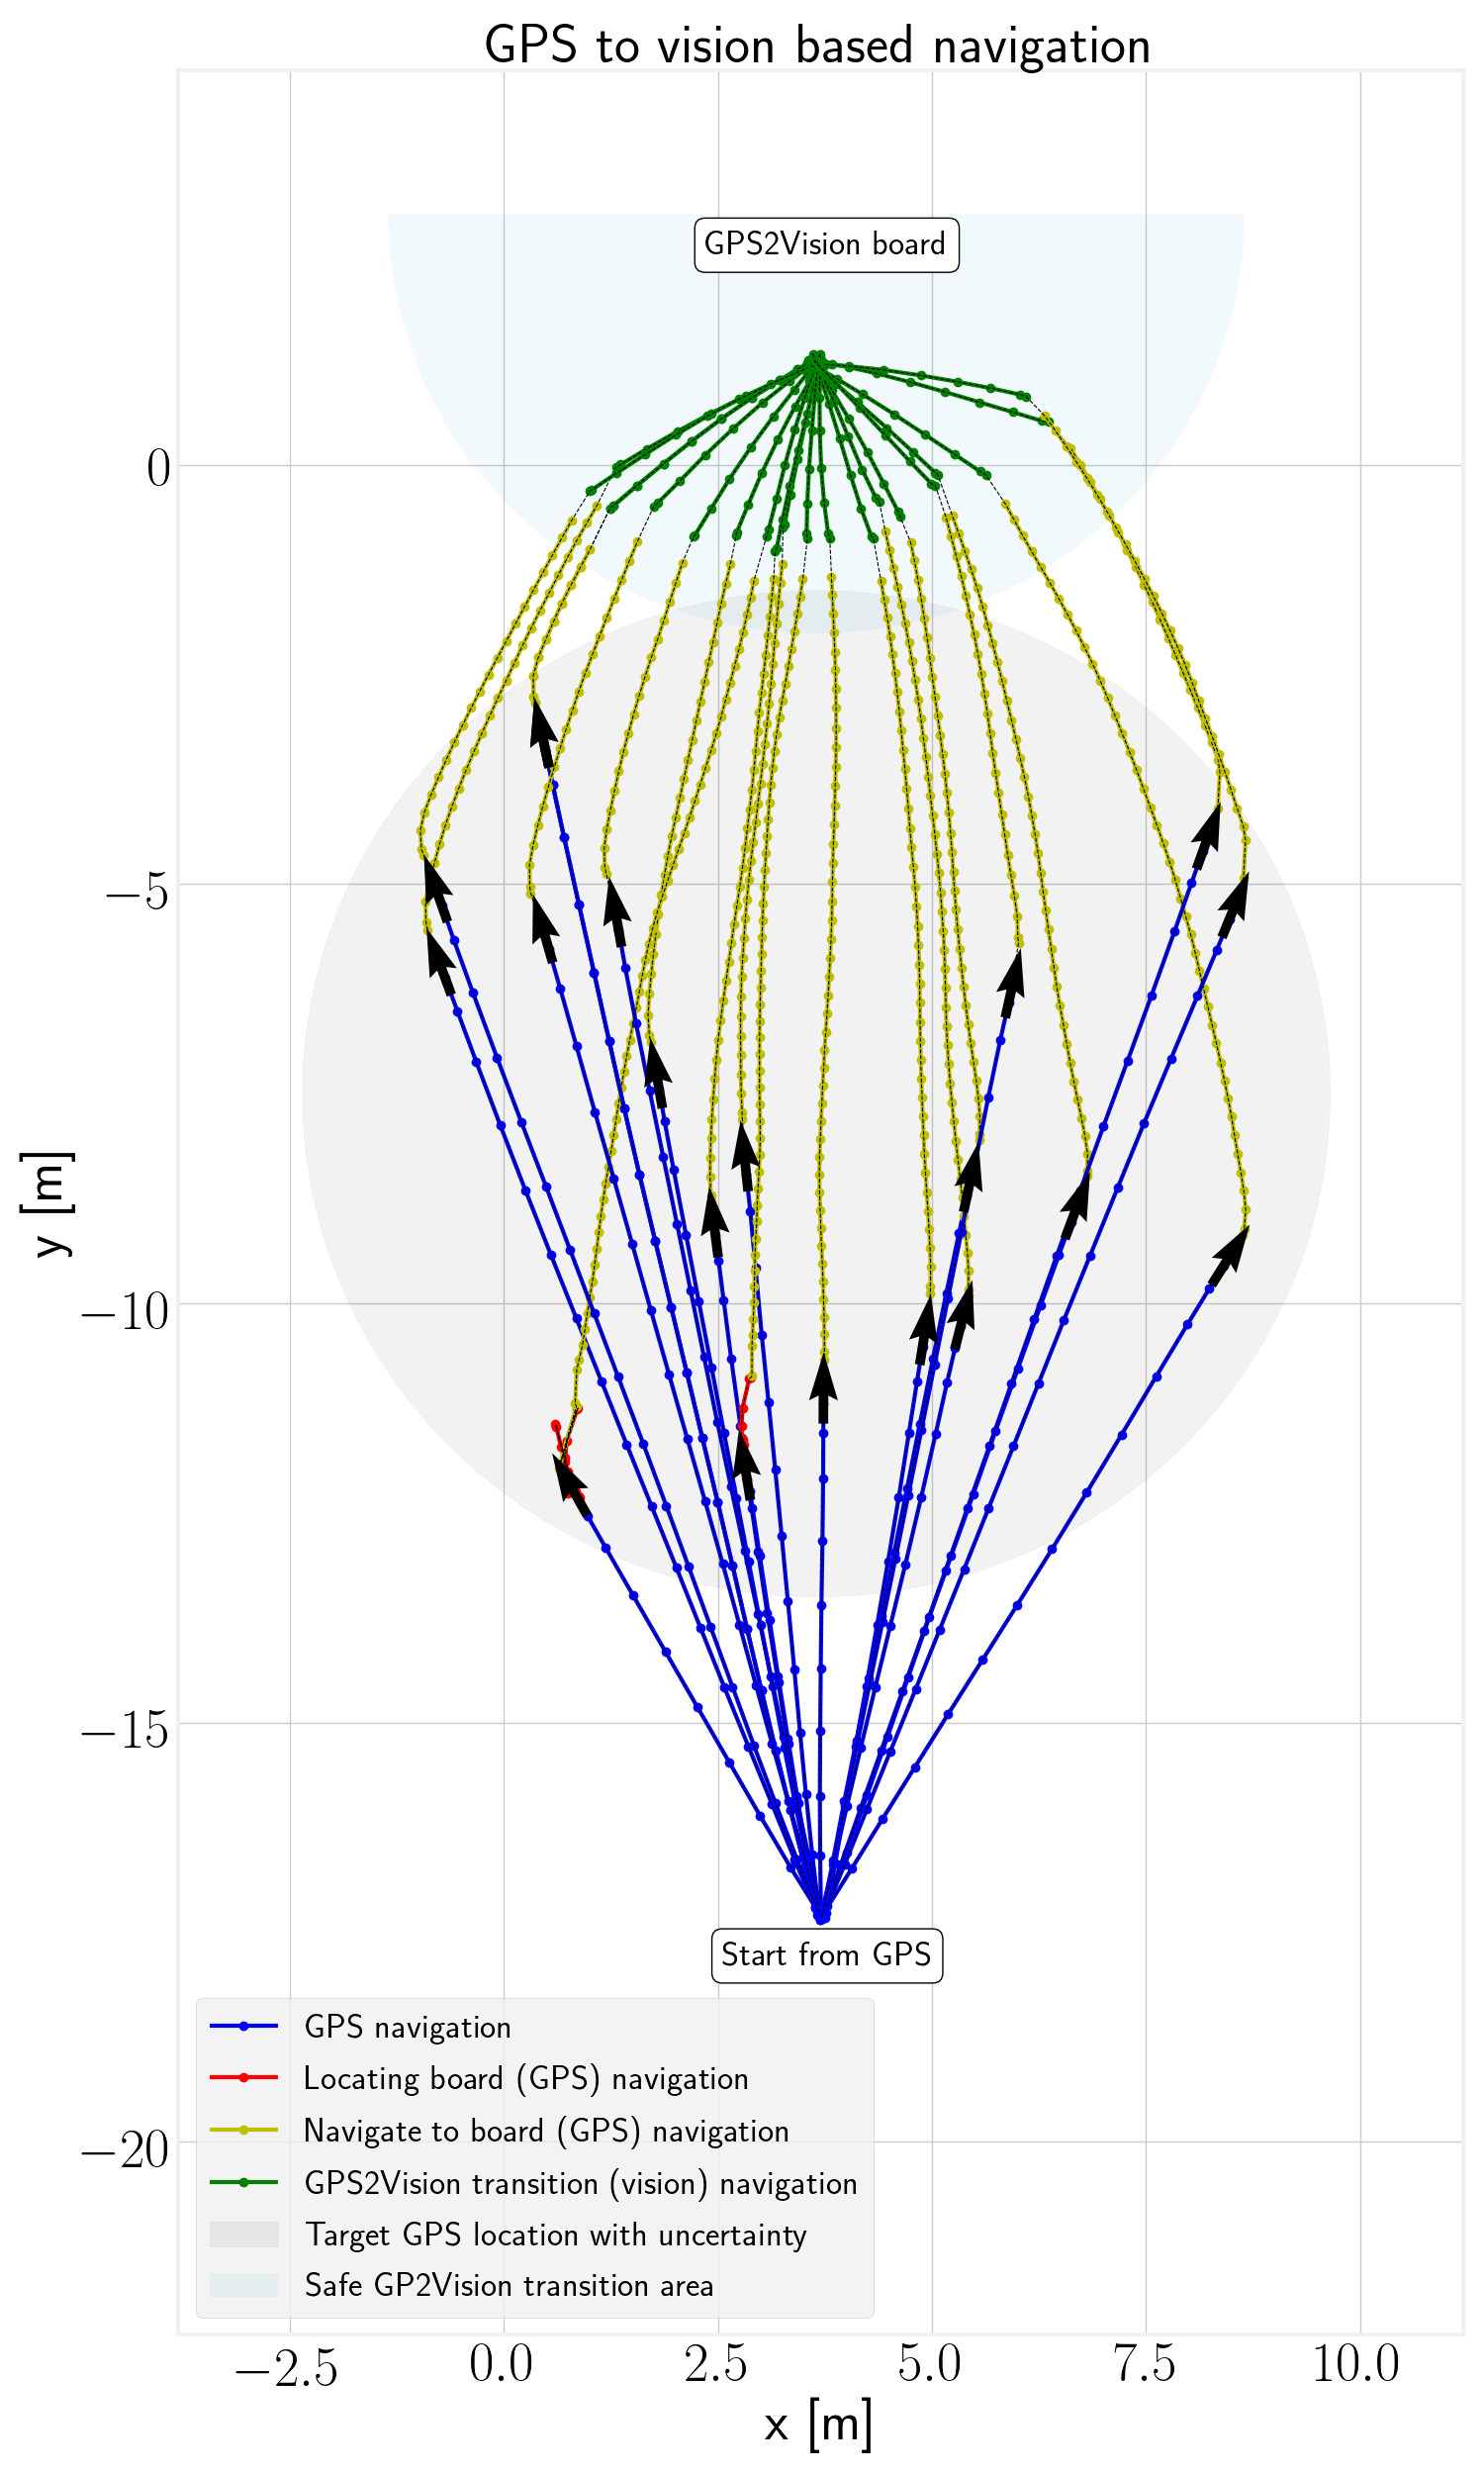
\includegraphics[width=\textwidth]{../Figures/GPS2Vision/test1_noWind_20_runs/gps2vision.png}
        \caption{}
        \label{fig:GPS2Vision_test1}
    \end{subfigure}
     \hspace{0.2em}
    \begin{subfigure}[t]{.45\textwidth}
        \centering
        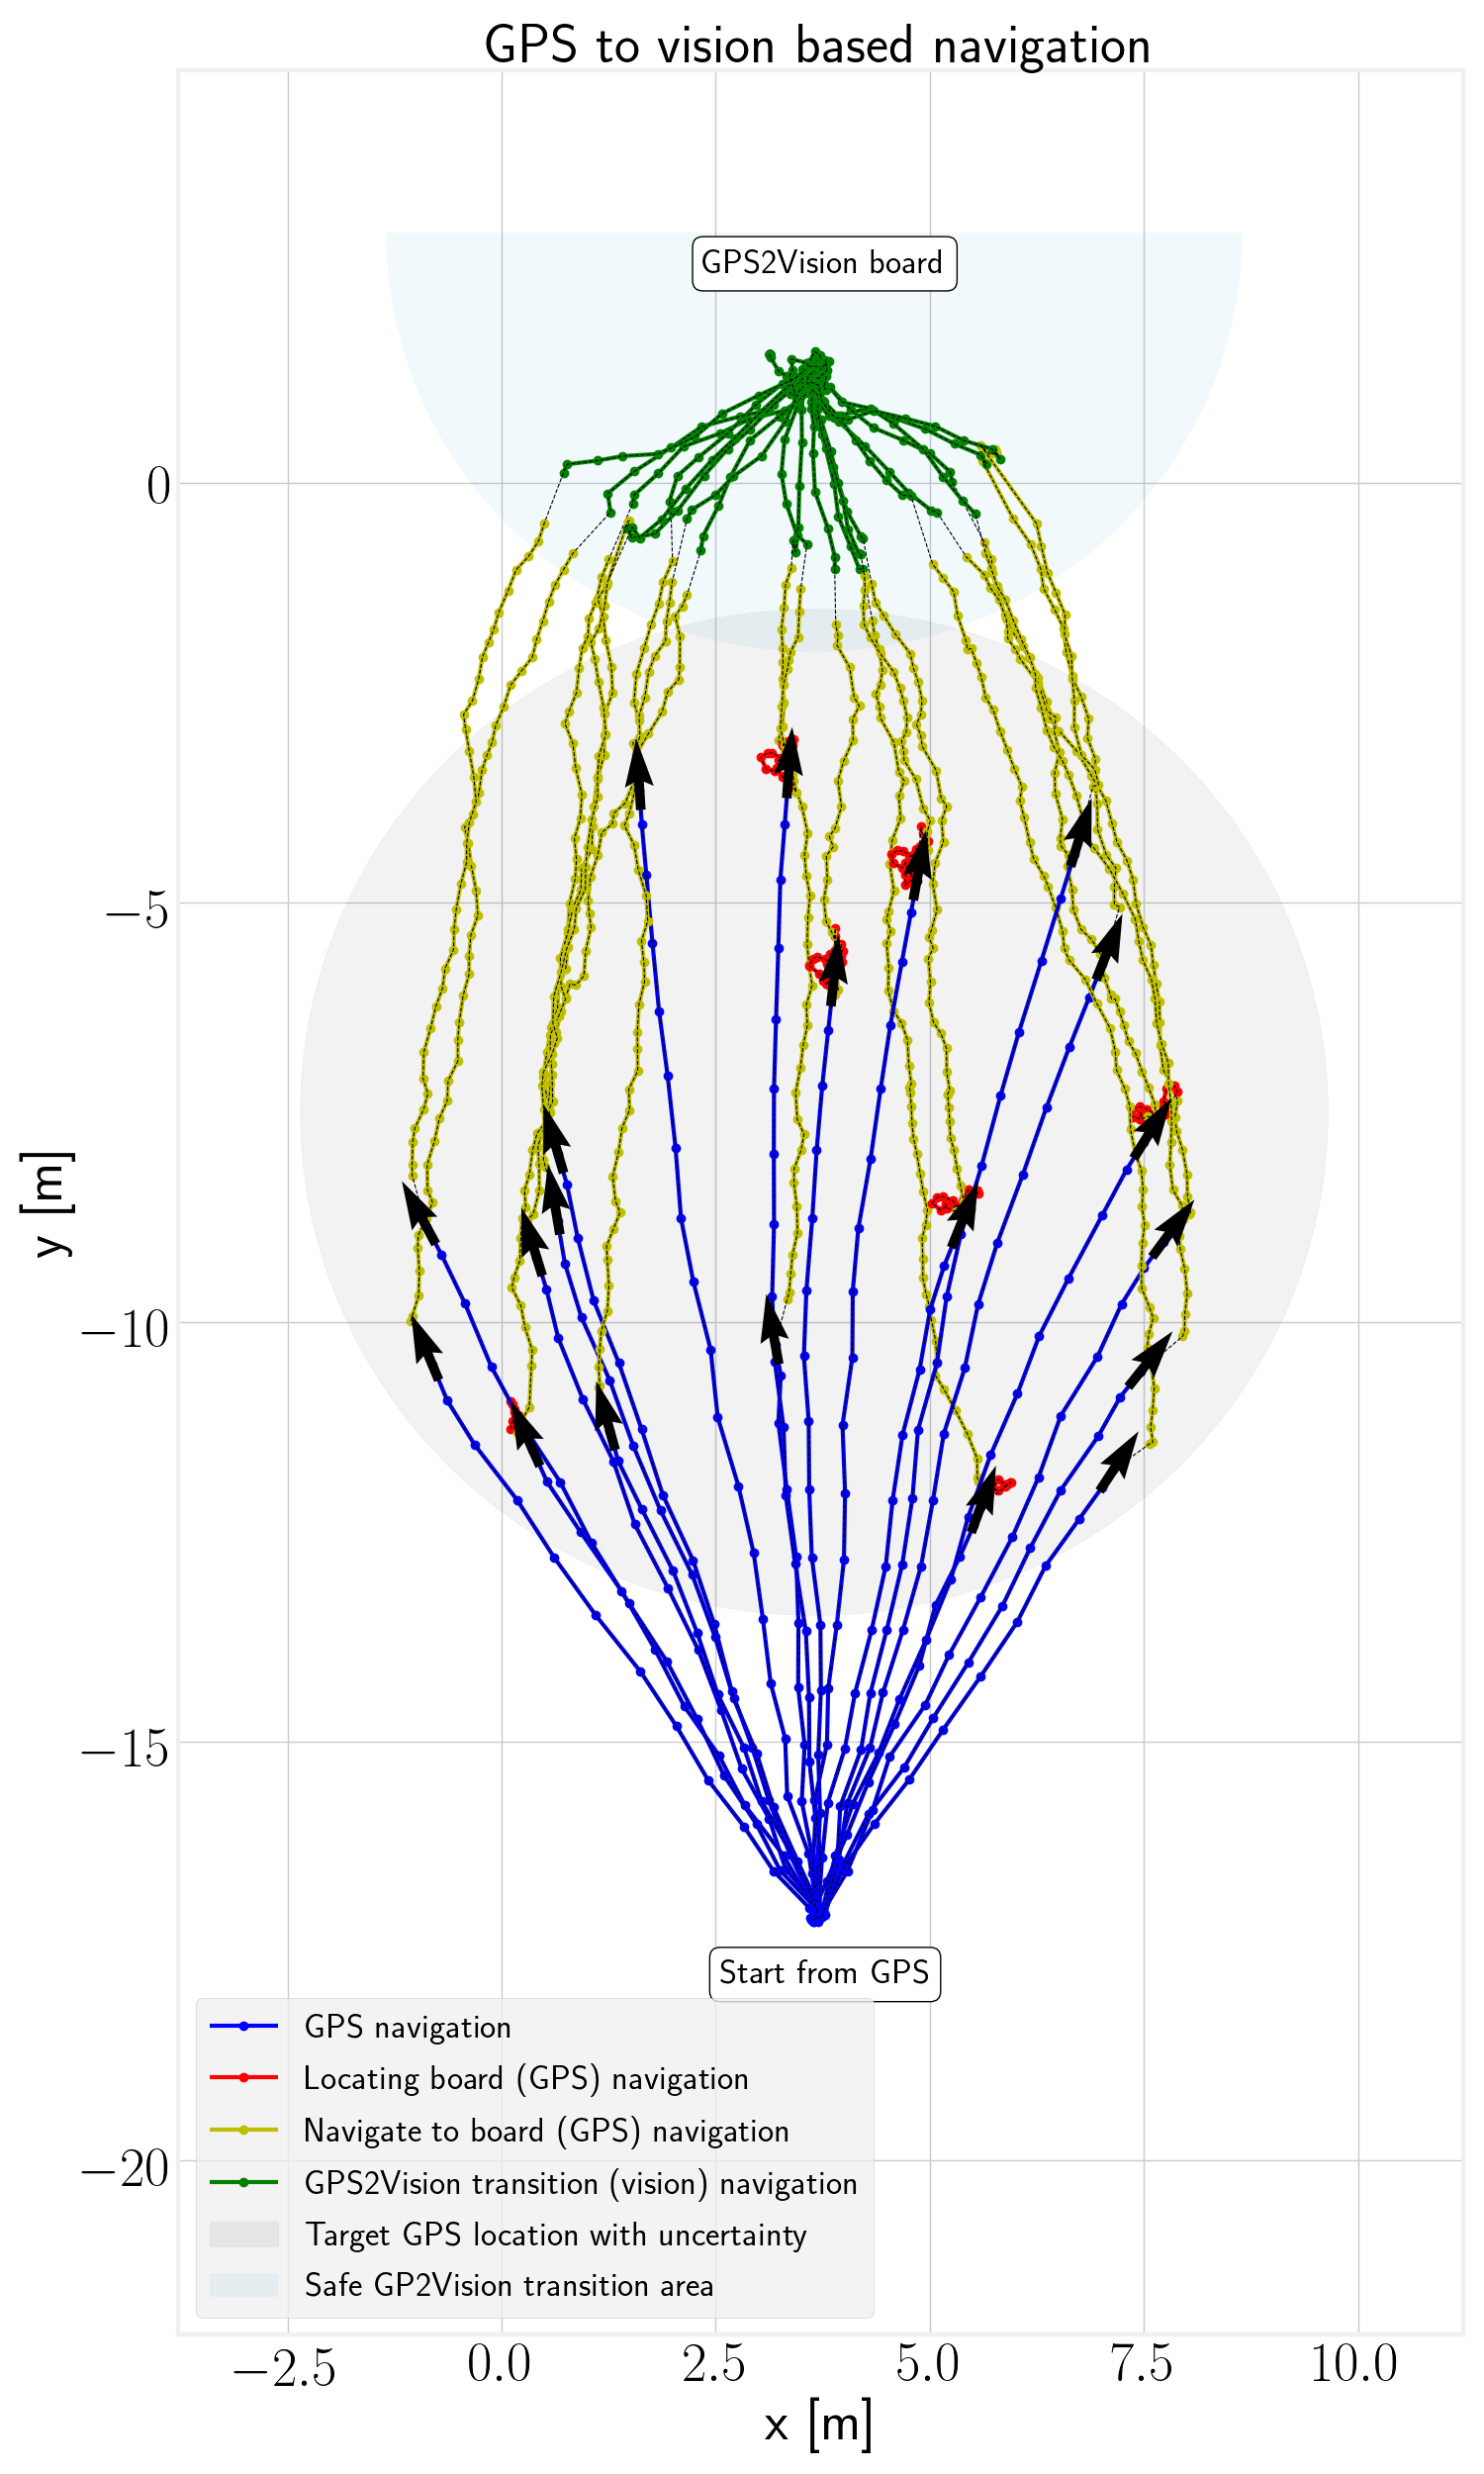
\includegraphics[width=\textwidth]{../Figures/GPS2Vision/test3_7-10ms_wind_20_runs/gps2vision.png}
        \caption{}
        \label{fig:GPS2Vision_test3}
    \end{subfigure}
    \caption{}
    \label{fig:GPS2Vision_test1_test3}
\end{figure}

\subsubsection{Vision based navigation}
\label{sec:vision_based_navigation}

\begin{figure}[H]
    \centering
    \begin{subfigure}[t]{.30\textwidth}
        \centering
        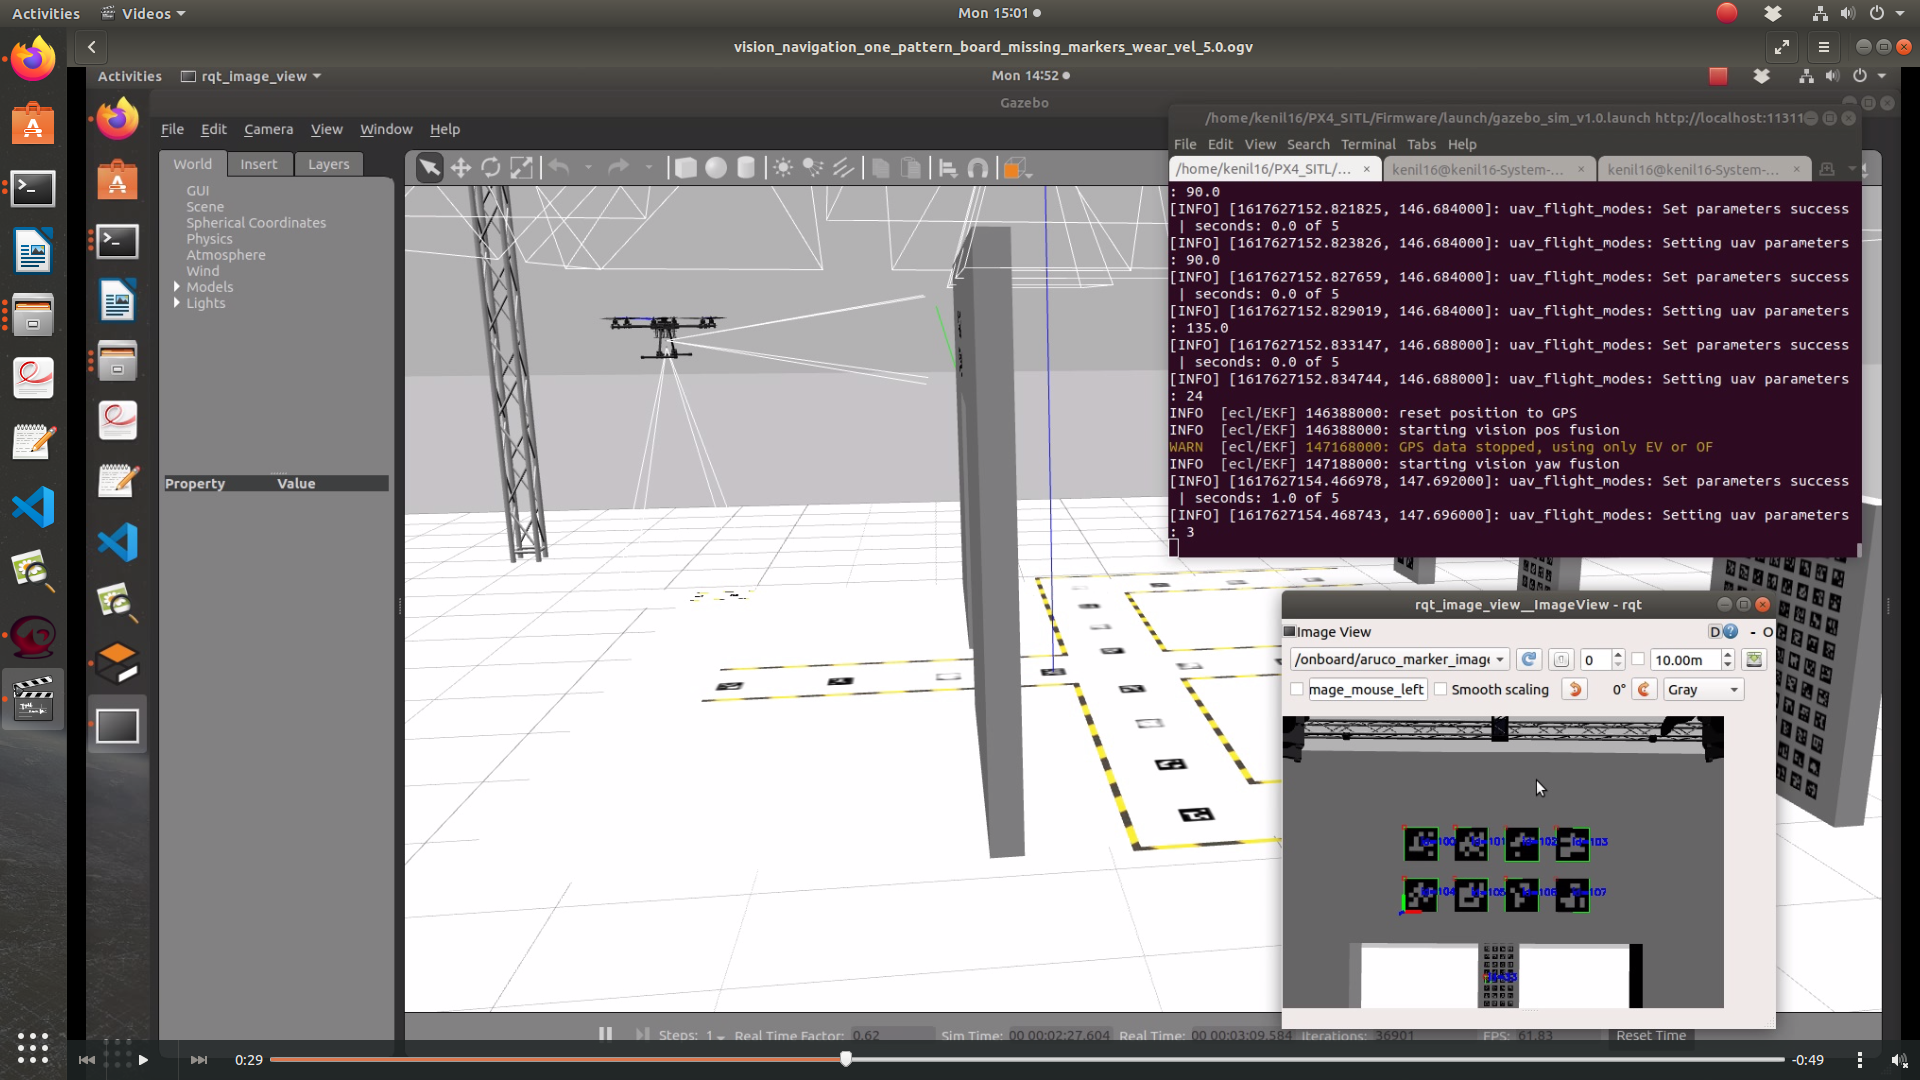
\includegraphics[width=\textwidth]{../Figures/vision_navigation/gps2vision.png}
        \caption{}
        \label{fig:vision_navigation_gps2vision}
    \end{subfigure}
     \hspace{0.2em}
    \begin{subfigure}[t]{.30\textwidth}
        \centering
        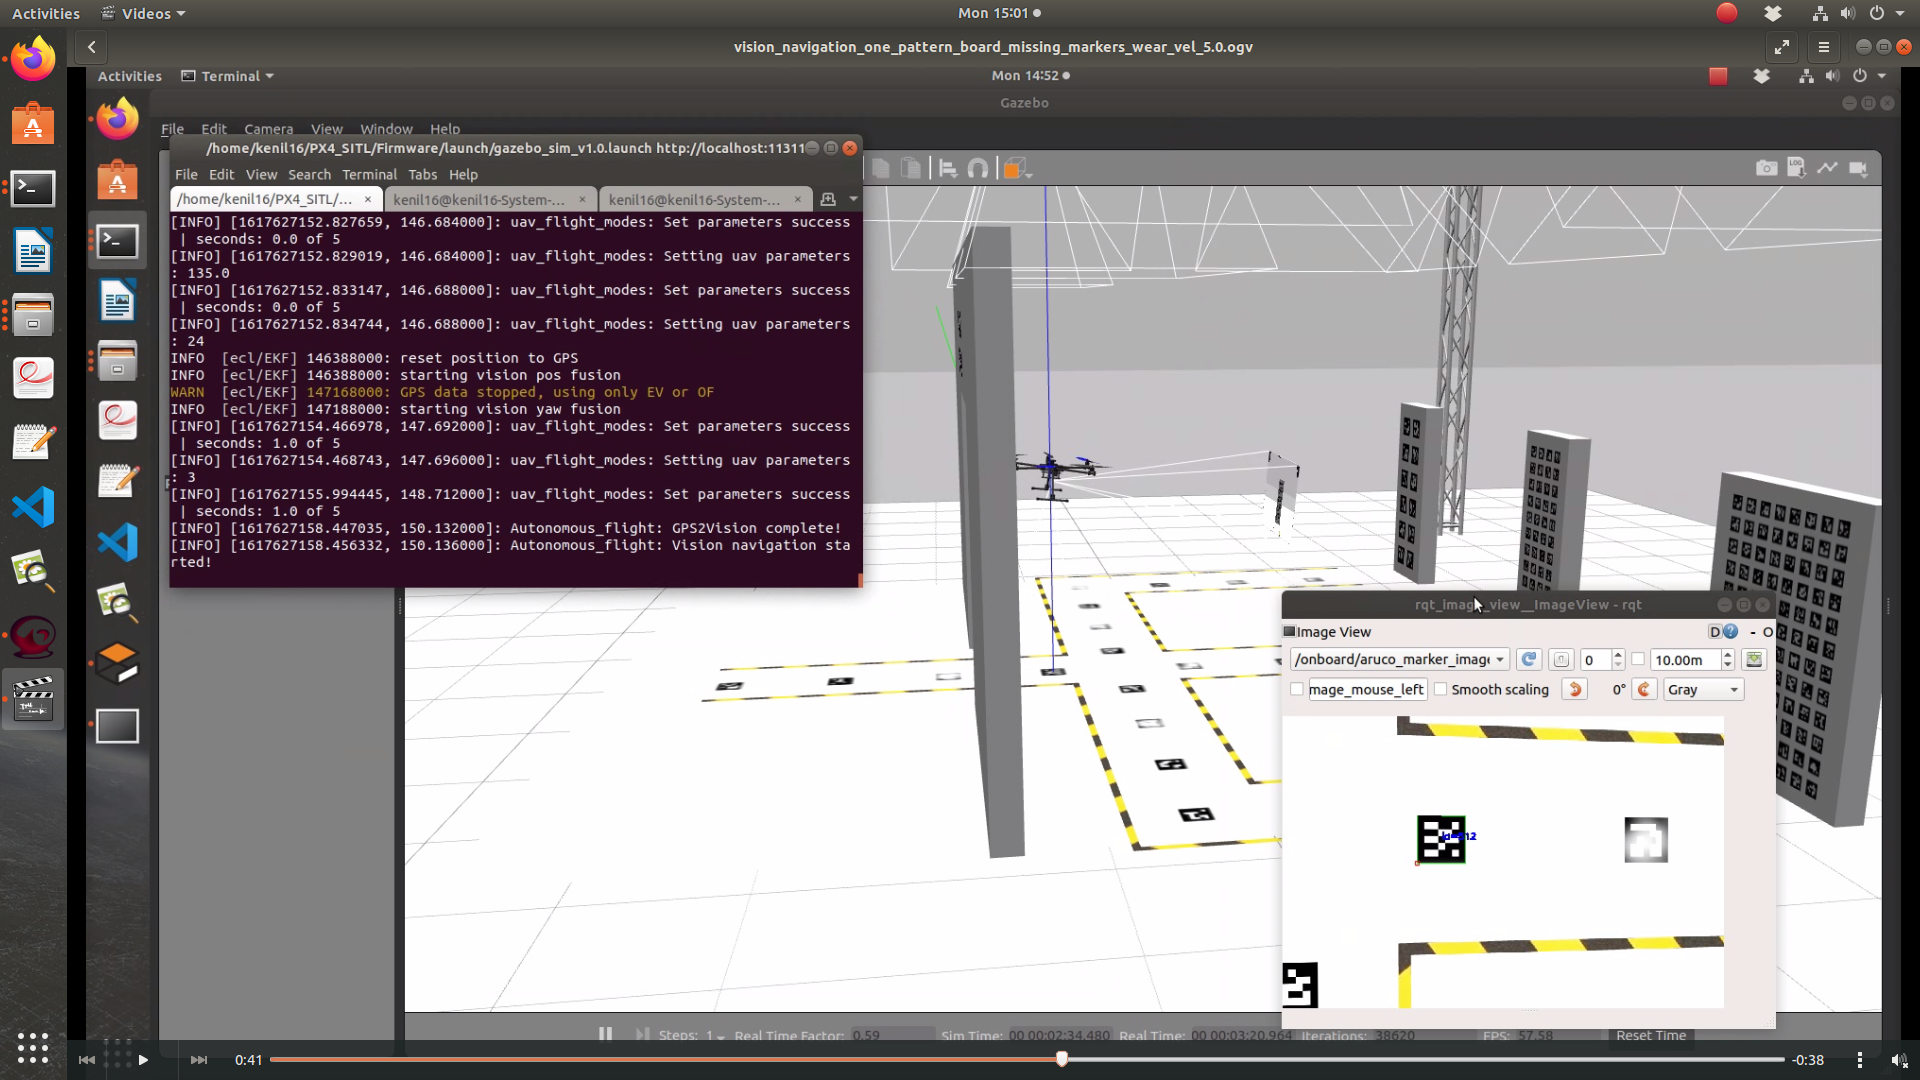
\includegraphics[width=\textwidth]{../Figures/vision_navigation/vision_navigation_one.png}
        \caption{}
        \label{fig:vision_navigation_vision_navigation_one}
    \end{subfigure}
     \hspace{0.2em}
    \begin{subfigure}[t]{.30\textwidth}
        \centering
        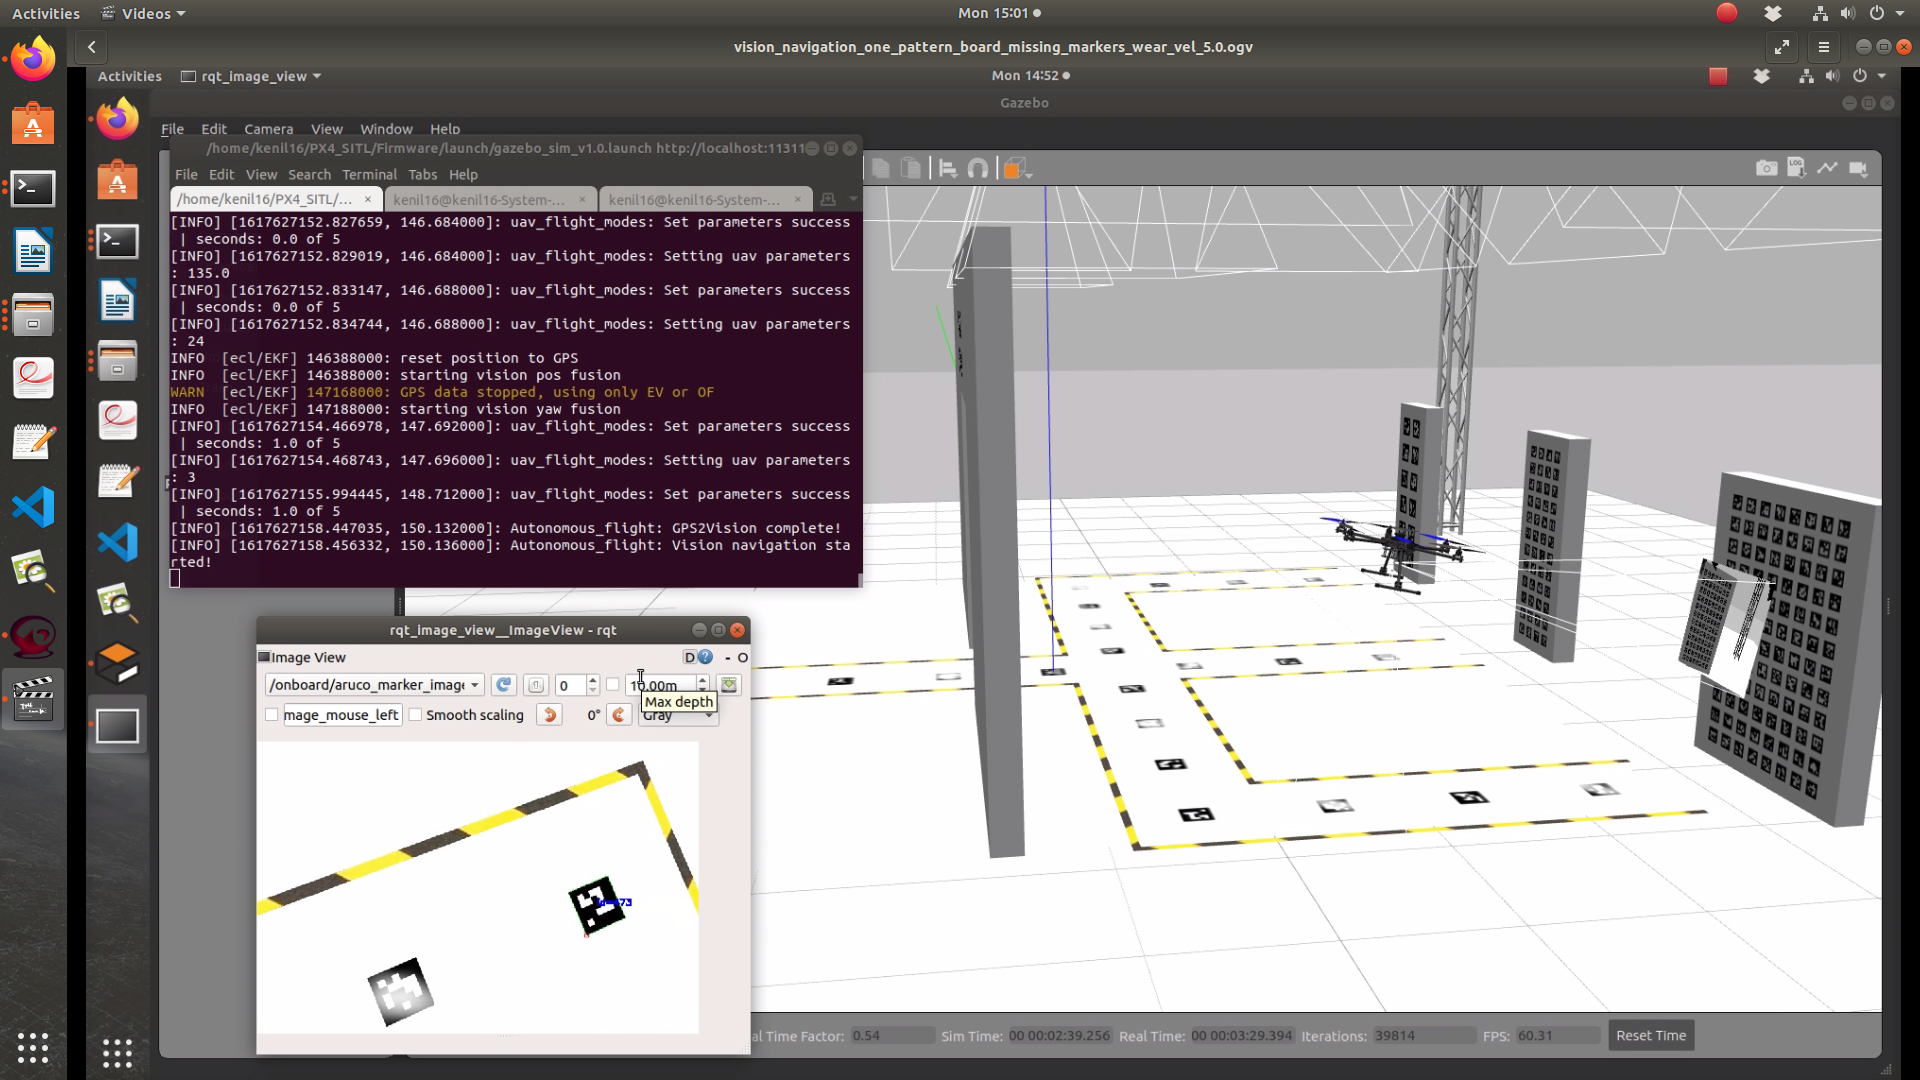
\includegraphics[width=\textwidth]{../Figures/vision_navigation/vision_navigation_two.png}
        \caption{}
        \label{fig:vision_navigation_vision_navigation_two}
    \end{subfigure}
    \caption{}
    \label{fig:vision_navigation}
\end{figure}

\begin{figure}[H]
    \centering
    \begin{subfigure}[t]{.20\textwidth}
        \centering
        \includegraphics[width=\textwidth]{../Figures/vision_navigation/grid_board_new_200_full.png}
        \caption{}
        \label{fig:vision_navigation_full_pattern_board}
    \end{subfigure}
     \hspace{0.2em}
    \begin{subfigure}[t]{.20\textwidth}
        \centering
        \includegraphics[width=\textwidth]{../Figures/vision_navigation/grid_board_new_200_big_onepattern.png}
        \caption{}
        \label{fig:vision_navigation_one_pattern_board}
    \end{subfigure}
     \hspace{0.2em}
    \begin{subfigure}[t]{.20\textwidth}
        \centering
        \includegraphics[width=\textwidth]{../Figures/vision_navigation/grid_board_new_200_big_onepattern_missing_markers1.png}
        \caption{}
        \label{fig:vision_navigation_one_pattern_board_missing_markers}
    \end{subfigure}
         \hspace{0.2em}
    \begin{subfigure}[t]{.20\textwidth}
        \centering
        \includegraphics[width=\textwidth]{../Figures/vision_navigation/grid_board_new_200_big_onepattern_missing_markers_wear.png}
        \caption{}
        \label{fig:vision_navigation_one_pattern_board_missing_markers_wear}
    \end{subfigure}
    \caption{}
    \label{fig:vision_navigation_boards}
\end{figure}

\begin{table}[H]
    \centering
    \addtolength{\leftskip} {-2cm}
    \addtolength{\rightskip}{-2cm}
        \caption{Statistics of the results from landing tests }
        \pgfplotstabletypeset[normal,
                columns/eg/.style={
                column name={Runs},
                dec sep align
        }
        ]{ %
        Estimation error & eg & Waypoint error & Vel (Horizontal) & Mean position & STD position & Mean angle & STD angle\\
        \topmidheader{8}{\textbf{Test 1}}
        ArUco pose & 20 & $0.1 m$ & $1\frac{m}{s}$ & $2.44cm$ & $2.51cm$ & $1.59 ^{\circ}$ & $9.68^{\circ}$\\
        \midheader{8}{\textbf{Test 2}}
        ArUco pose & 20 & $0.1 m$ & $1\frac{m}{s}$ &$2.44cm$ & $2.29cm$ & $1.30 ^{\circ}$ & $7.44^{\circ}$\\
        \midheader{8}{\textbf{Test 3}}
        ArUco pose & 20 & $0.1 m$ & $1\frac{m}{s}$ & $3.19cm$ & $3.28cm$ & $1.99 ^{\circ}$ & $10.88^{\circ}$\\
        \midheader{8}{\textbf{Test 4}}
        ArUco pose & 20 & $0.1 m$ & $1\frac{m}{s}$ & $4.21cm$ & $3.96cm$ & $3.09 ^{\circ}$ & $11.99^{\circ}$\\
        \midheader{8}{\textbf{Test 5}}
        ArUco pose & 20 & $0.1 m$ & $5\frac{m}{s}$ & $5.66cm$ & $5.79cm$ & $6.89 ^{\circ}$ & $22.29^{\circ}$\\}
\end{table}

\begin{figure}[H]
    \centering
    \begin{subfigure}[t]{.30\textwidth}
        \centering
        \includegraphics[width=\textwidth]{../Figures/vision_navigation/test1_full_pattern_board/2d_path.png}
        \caption{}
        \label{fig:vision_navigation_2d_path_full_board}
    \end{subfigure}
     \hspace{0.2em}
    \begin{subfigure}[t]{.30\textwidth}
        \centering
        \includegraphics[width=\textwidth]{../Figures/vision_navigation/test4_one_pattern_missing_markers_wear_board/2d_path.png}
        \caption{}
        \label{fig:vision_navigation_2d_path_missing_markers_wear_vel_1.0}
    \end{subfigure}
     \hspace{0.2em}
    \begin{subfigure}[t]{.30\textwidth}
        \centering
        \includegraphics[width=\textwidth]{../Figures/vision_navigation/test5_one_pattern_missing_markers_wear_board/2d_path.png}
        \caption{}
        \label{fig:vision_navigation_2d_path_missing_markers_wear_vel_5.0}
    \end{subfigure}
    \caption{}
    \label{fig:vision_navigation_2d_path}
\end{figure}

\begin{figure}[H]
    \centering
    \begin{subfigure}[t]{.30\textwidth}
        \centering
        \includegraphics[width=\textwidth]{../Figures/vision_navigation/test1_full_pattern_board/error_x/pose_error_x_test1.png}
        \caption{}
        \label{fig:vision_navigation_error_x}
    \end{subfigure}
     \hspace{0.2em}
    \begin{subfigure}[t]{.30\textwidth}
        \centering
        \includegraphics[width=\textwidth]{../Figures/vision_navigation/test1_full_pattern_board/error_y/pose_error_y_test1.png}
        \caption{}
        \label{fig:vision_navigation_error_y}
    \end{subfigure}
     \hspace{0.2em}
    \begin{subfigure}[t]{.30\textwidth}
        \centering
        \includegraphics[width=\textwidth]{../Figures/vision_navigation/test1_full_pattern_board/error_z/pose_error_z_test1.png}
        \caption{}
        \label{fig:vision_navigation_error_z}
    \end{subfigure}
    \caption{}
    \label{fig:vision_navigation_error_pos}
\end{figure}

\begin{figure}[H]
    \centering
    \begin{subfigure}[t]{.30\textwidth}
        \centering
        \includegraphics[width=\textwidth]{../Figures/vision_navigation/test1_full_pattern_board/error_roll/pose_error_roll_test1.png}
        \caption{}
        \label{fig:vision_navigation_error_roll}
    \end{subfigure}
     \hspace{0.2em}
    \begin{subfigure}[t]{.30\textwidth}
        \centering
        \includegraphics[width=\textwidth]{../Figures/vision_navigation/test1_full_pattern_board/error_pitch/pose_error_pitch_test1.png}
        \caption{}
        \label{fig:vision_navigation_error_pitch}
    \end{subfigure}
     \hspace{0.2em}
    \begin{subfigure}[t]{.30\textwidth}
        \centering
        \includegraphics[width=\textwidth]{../Figures/vision_navigation/test1_full_pattern_board/error_yaw/pose_error_yaw_test1.png}
        \caption{}
        \label{fig:vision_navigation_error_yaw}
    \end{subfigure}
    \caption{}
    \label{fig:vision_navigation_error_angle}
\end{figure}

\subsubsection{Vision based landing}
\label{sec:vision_based_landing}

\begin{figure}[H]
    \centering
    \begin{subfigure}[t]{.30\textwidth}
        \centering
        \includegraphics[width=\textwidth]{../Figures/landing_test/landing_station_one.png}
        \caption{}
        \label{fig:vision_based_landing_landing_station_one}
    \end{subfigure}
     \hspace{0.2em}
    \begin{subfigure}[t]{.30\textwidth}
        \centering
        \includegraphics[width=\textwidth]{../Figures/landing_test/landing_station_two.png}
        \caption{}
        \label{fig:vision_based_landing_landing_station_two}
    \end{subfigure}
     \hspace{0.2em}
    \begin{subfigure}[t]{.30\textwidth}
        \centering
        \includegraphics[width=\textwidth]{../Figures/landing_test/landing_station_three.png}
        \caption{}
        \label{fig:vision_based_landing_landing_station_three}
    \end{subfigure}
    \caption{}
    \label{fig:vision_based_landing_landing_stations}
\end{figure}

\begin{table}[H]
    \centering
    \addtolength{\leftskip} {-2cm}
    \addtolength{\rightskip}{-2cm}
        \caption{Statistics of the results from landing tests }
        \pgfplotstabletypeset[normal,
                columns/eg/.style={
                column name={Runs},
                dec sep align
        }
        ]{ %
        Station & eg & Waypoint error & Velocity & Min & Max & Mean & STD & Stabilize time & Landing time\\
        \topmidheader{11}{\textbf{Test 1}}
        One         & 35      & $0.1 m$ & $0.1 \frac{m}{s}$ & $1.60cm$ & $12.46cm$ & $5.81cm$ & $3.02cm$ & $3.60s$ &$11.51s$\\
        two         & 30     & $0.1 m$ & $0.1 \frac{m}{s}$ & $0.70cm$ & $11.83 cm$& $5.79cm$ & $2.54cm$& $0.70s$ &$11.76s$\\     
        Three       & 35     & $0.1 m$ & $0.1 \frac{m}{s}$ & $0.62cm$ & $10.75cm$ & $5.86cm$ & $2.50cm$& $3.22s$ &$11.82s$\\    
        \midheader{11}{\textbf{Test 2}}
        One         & 33      & $0.1 m$ & $0.5 \frac{m}{s}$ & $2.20cm$ & $15.04cm$ & $8.00cm$ & $2.67cm$ & $2.63s$ &$3.00s$\\
        two         & 29     & $0.1 m$ & $0.5 \frac{m}{s}$ & $3.18cm$ & $11.60 cm$& $7.62cm$ & $2.19cm$& $0.20s$ &$3.00s$\\     
        Three       & 38     & $0.1 m$ & $0.5 \frac{m}{s}$ & $1.11cm$ & $14.63cm$ & $7.87cm$ & $3.25cm$& $2.18s$ &$3.02s$\\    
        \midheader{11}{\textbf{Test 3}}
        One         & 32      & $0.1 m$ & $0.9 \frac{m}{s}$ & $4.63cm$ & $14.01cm$ & $9.25cm$ & $2.27cm$ & $1.68s$ &$2.15s$\\
        two         & 36    & $0.1 m$ & $0.9 \frac{m}{s}$ & $4.79cm$ & $14.00 cm$& $9.54cm$ & $1.92cm$& $0.19s$ &$2.13s$\\     
        Three       & 32     & $0.1 m$ & $0.9 \frac{m}{s}$ & $3.35cm$ & $18.45cm$ & $9.45cm$ & $2.88cm$& $2.09s$ &$2.18s$\\}
\end{table}

\begin{table}[H]
    \centering
    \addtolength{\leftskip} {-2cm}
    \addtolength{\rightskip}{-2cm}
        \caption{Statistics of the results from landing tests }
        \pgfplotstabletypeset[normal,
                columns/eg/.style={
                column name={Runs},
                dec sep align
        }
        ]{ %
        Station & eg & Waypoint error & Velocity & Min & Max & Mean & STD & Stabilize time & Landing time\\
        \topmidheader{11}{\textbf{Test 4}}
One         & 33      & $0.05 m$ & $0.1 \frac{m}{s}$ & $0.08cm$ & $9.46cm$ & $4.81cm$ & $2.15cm$ & $9.93s$ &$11.45s$\\
        two         & 33    & $0.05 m$ & $0.1 \frac{m}{s}$ & $0.97cm$ & $11.18 cm$& $4.74cm$ & $2.56cm$& $6.96s$ &$11.69s$\\     
        Three       & 34     & $0.05 m$ & $0.1 \frac{m}{s}$ & $0.19cm$ & $11.84cm$ & $4.54cm$ & $2.41cm$& $9.11s$ &$11.58s$\\        		\midheader{11}{\textbf{Test 5}}
        One         & 32     & $0.05 m$ & $0.5 \frac{m}{s}$ & $1.63cm$ & $9.84cm$ & $5.25cm$ & $2.36cm$ & $8.43s$ &$3.00s$\\
        two         & 32    & $0.05 m$ & $0.5 \frac{m}{s}$ & $1.31cm$ & $13.07 cm$& $5.98cm$ & $2.90cm$& $6.34s$ &$3.00s$\\     
        Three       & 36     & $0.05 m$ & $0.5 \frac{m}{s}$ & $0.45cm$ & $12.22cm$ & $4.98cm$ & $2.88cm$& $9.33s$ &$3.00s$\\				\midheader{11}{\textbf{Test 6}}
        One         & 32     & $0.05 m$ & $0.9 \frac{m}{s}$ & $0.20cm$ & $11.89cm$ & $4.96cm$ & $2.77cm$ & $9.18s$ &$2.28s$\\
        two         & 35    & $0.05 m$ & $0.9 \frac{m}{s}$ & $0.65cm$ & $14.13 cm$& $5.90cm$ & $3.32cm$& $5.91s$ &$2.34s$\\     
        Three       & 33     & $0.05 m$ & $0.9 \frac{m}{s}$ & $1.06cm$ & $13.54cm$ & $5.35cm$ & $2.70cm$& $8.54s$ &$2.36s$\\}
\end{table}


\begin{figure}[H]
    \centering
    \begin{subfigure}[t]{.30\textwidth}
        \centering
        \includegraphics[width=\textwidth]{../Figures/landing_test/test3_speed_0.9_error_0.1/landing_for_station_one.png}
        \caption{}
        \label{fig:vision_based_landing_landing_station_one_test3}
    \end{subfigure}
     \hspace{0.2em}
    \begin{subfigure}[t]{.30\textwidth}
        \centering
        \includegraphics[width=\textwidth]{../Figures/landing_test/test3_speed_0.9_error_0.1/landing_for_station_two.png}
        \caption{}
        \label{fig:vision_based_landing_landing_station_two_test3}
    \end{subfigure}
     \hspace{0.2em}
    \begin{subfigure}[t]{.30\textwidth}
        \centering
        \includegraphics[width=\textwidth]{../Figures/landing_test/test3_speed_0.9_error_0.1/landing_for_station_three.png}
        \caption{}
        \label{fig:vision_based_landing_landing_station_three_test3}
    \end{subfigure}
    \caption{}
    \label{fig:vision_based_landing_test3}
\end{figure}

\begin{figure}[H]
    \centering
    \begin{subfigure}[t]{.30\textwidth}
        \centering
        \includegraphics[width=\textwidth]{../Figures/landing_test/test4_speed_0.1_error_0.05/landing_for_station_one.png}
        \caption{}
        \label{fig:vision_based_landing_landing_station_one_test4}
    \end{subfigure}
     \hspace{0.2em}
    \begin{subfigure}[t]{.30\textwidth}
        \centering
        \includegraphics[width=\textwidth]{../Figures/landing_test/test4_speed_0.1_error_0.05/landing_for_station_two.png}
        \caption{}
        \label{fig:vision_based_landing_landing_station_two_test4}
    \end{subfigure}
     \hspace{0.2em}
    \begin{subfigure}[t]{.30\textwidth}
        \centering
        \includegraphics[width=\textwidth]{../Figures/landing_test/test4_speed_0.1_error_0.05/landing_for_station_three.png}
        \caption{}
        \label{fig:vision_based_landing_landing_station_three_test4}
    \end{subfigure}
    \caption{}
    \label{fig:vision_based_landing_test4}
\end{figure}

\end{document}